\documentclass[11pt, a4paper, oldfontcommands]{memoir}

\usepackage[utf8]{inputenc}
\usepackage[T1]{fontenc}
\usepackage[french]{babel}
\usepackage{url}


\usepackage{microtype}
\usepackage[table]{xcolor}
%\usepackage{newcent}
\usepackage{mathpazo}
%\usepackage{ebgaramond}
\usepackage{booktabs}
\usepackage{caption}
\usepackage{subcaption}
\usepackage{listings}
\usepackage{todo}

\usepackage{mathtools}

\usepackage{algpseudocode}
\usepackage{algorithmicx}
\usepackage{algorithm}

\usepackage{float}

\usepackage{marginnote}

\usepackage{tablefootnote}
\usepackage{multirow}

\usepackage{xparse}
\usepackage[outputdir=out]{minted}

\usepackage{graphicx}
\graphicspath{{graphics/}{graphics/figures/}}

\usepackage{tikz}
\usetikzlibrary{shapes}

\usepackage[
breaklinks=true,colorlinks=true,
linkcolor=black,urlcolor=black,citecolor=black,% PRINT
bookmarks=true,bookmarksopenlevel=2]{hyperref}
% \makeatletter\let\@bibitem\saved@bibitem\makeatother

\usepackage{geometry}
% PDF VIEW
% \geometry{total={210mm,297mm},
% left=35mm,right=35mm,%
% bindingoffset=0mm, top=35mm,bottom=35mm}
% PRINT
%\geometry{total={210mm,297mm}, left=35mm, right=35mm, bindingoffset=15mm, top=40mm, bottom=40mm}

%\usepackage{minitoc}

\usepackage{tabularx}
\definecolor{codegreen}{rgb}{0,0.6,0}
\definecolor{codegray}{rgb}{0.5,0.5,0.5}
\definecolor{codepurple}{rgb}{0.58,0,0.82}
\definecolor{backcolour}{rgb}{0.95,0.95,0.92}
\usepackage{footnote}
\makesavenoteenv{tabular}


\lstdefinestyle{mystyle}{
    backgroundcolor=\color{backcolour},   
    commentstyle=\color{codegreen},
    keywordstyle=\color{magenta},
    numberstyle=\tiny\color{codegray},
    stringstyle=\color{codepurple},
    basicstyle=\ttfamily\footnotesize,
    breakatwhitespace=false,         
    breaklines=true,                 
    captionpos=b,                    
    keepspaces=true,                 
    numbers=left,                    
    numbersep=5pt,                  
    showspaces=false,                
    showstringspaces=false,
    showtabs=false,                  
    tabsize=2
}
 
\lstset{style=mystyle}
%\OnehalfSpacing
\linespread{1.2}

% \usepackage[style=numeric, maxbibnames=6]{biblatex}

%%% CHAPTER'S STYLE
%\chapterstyle{bianchi}
\chapterstyle{veelo}
%\chapterstyle{ger}
%\chapterstyle{madsen}
%\chapterstyle{ell}
%\chapterstyle{wilsondob}
% \chapterstyle{thatcher}
%\chapterstyle{pedersen}
%%% STYLE OF SECTIONS, SUBSECTIONS, AND SUBSUBSECTIONS
\setsecheadstyle{\Large\bfseries\raggedright}
\setsubsecheadstyle{\large\bfseries\raggedright}
\setsubsubsecheadstyle{\bfseries\raggedright}


%%% STYLE OF PAGES NUMBERING
%pagestyle{companion}\nouppercaseheads 
\pagestyle{headings}
%\pagestyle{Ruled}
%\pagestyle{plain}
%\makepagestyle{heading}
%\makeevenfoot{plain}{\thepage}{}{}
%\makeoddfoot{plain}{}{}{\thepage}
\makeevenhead{plain}{}{}{}
\makeoddhead{plain}{}{}{}

\setlength{\parskip}{0.3cm}
\maxsecnumdepth{subsection} % chapters, sections, and subsections are numbered
\maxtocdepth{subsection} % chapters, sections, and subsections are in the Table of Contents

%\mtcselectlanguage{french}
\usepackage{enumitem}

% ==========================================
% Long dash
% ==========================================
\ExplSyntaxOn
\NewDocumentCommand{\longdash}{ O{2} }
 {
  --\prg_replicate:nn { #1 - 1 } { \negthinspace -- }
 }
\ExplSyntaxOff

% ===========================================
% Program names
% ===========================================
\newcommand\mibench{\textsc{MiBench}\xspace}
\newcommand\parsec{\textsc{PARSEC}\xspace}
\newcommand\valgrind{\textsc{Valgrind}\xspace}

% ===========================================
% Table stuff
% ===========================================
\newcommand\tcheck{$\times$}
\newcommand\tpros{v}
\newcommand\tcons{x}

% \addbibresource{Bibliography.bib}

\begin{document}
% \firstchapteris{1}
% \dominitoc

% \newenvironment{keypoints}{
%     \begin{center}
%     \begin{tabular}{p{0.95\textwidth}}
%     \cellcolor{teal!25}\rule{0pt}{20pt}
%     \textbf{Points clés pour nos travaux} \\
%     \cellcolor{gray!10}
%     \begin{itemize}
%         \renewcommand{\labelitemi}{$\square$}
% }{
%     \end{itemize} \\
%     \end{tabular}
%     \end{center}
% }

\renewcommand{\labelitemi}{$\bullet$}
\renewcommand{\labelitemii}{$\bullet$}
\renewcommand{\labelitemiii}{$\bullet$}
\renewcommand{\labelitemiv}{$\bullet$}

\renewcommand{\theequation}{\arabic{section}.\Roman{equation}}


% - - - - - - - d�but de la page 
\thispagestyle{empty}

%\includegraphics[scale=0.12]{upmc-logo.png}

{\


\begin{center}

% \vspace*{0.5cm}

TH\`ESE DE DOCTORAT DE \\ \textbf{SORBONNE UNIVERSIT\'E}


Sp\'ecialit\'e
\textbf{Informatique}\ \\ 

%\vspace*{0.5cm}

\'Ecole doctorale Informatique, T\'el\'ecommunications et \'Electronique (Paris)

%\vspace*{1cm}


Pr\'esent\'ee par \ \\


{\Large \textbf{C\'edric COURTAUD}}

Pour obtenir le grade de \ \\[1ex]
\textbf{DOCTEUR de Sorbonne Universit\'e} \ \\

% \vspace*{0.5cm}

\end{center}

\rule{\linewidth}{1pt}
{\Large 
 \begin{center}
	\textbf{Caract\'erisation de la sensibilit\'e \\ aux  interf\'erences m\'emoire dans les syst\`emes temps-r\'eels embarqu\'es sur des plateformes multi-c\oe{}urs}
 \end{center}
 }
\rule{\linewidth}{1pt}

\


% \vspace*{1.5cm} 
\begin{center}
{\bf Soutenue le 28 janvier 2020 devant le jury compos\'e de } 
 {\begin{tabular}{lll}
 	% \hline
 	& & \\
    Gilles {\sc Grimaud} & {\it Rapporteur} & Professeur, Universit\'e de Lille 1 \\
    Daniel {\sc Hagimont} & {\it Rapporteur} & Professeur, INPT/ENSHEITT \\
    Liliana {\sc Cucu-Grosjean} & {\it Examinateur} &Charg\'ee de recherche, Inria \\
    Lionel {\sc Lacassagne} & {\it Examinateur} & Professeur, Sorbonne Universit\'e \\
    Isabelle {\sc Puaut} & {\it Examinateur} & Professeur, Universit\'e de Rennes 1 \\
    Gilles {\sc Muller} & {\it Directeur de th\`ese} & Directeur de recherche, Inria \\
    Daniel {\sc Gracia P\'erez} &  {\it Encadrant} &Ing\'enieur de recherche, Thales \\
    Julien {\sc Sopena} & {\it Encadrant} & Maitre de conf\'erence, Sorbonne Universit\'e\\
 	% \hline
 \end{tabular}
 }

\end{center}

}
\cleardoublepage

\frontmatter


\chapter*{Remerciements}

Beaucoup de personnes ont contribuées directement ou indirectement à rendre ce manuscrit possible. Je tiens ici à les remercier.

Tout d'abords, un grand merci à mes rapporteurs, Gilles Grimaud et Daniel Hagimont, pour le temps qu'ils ont consacré à l'examen de ce document et pour leur commentaires et leur avis. J'addresse également mes remerciements à Liliana Cucu-Grosjean, Lionel Lacassagne et Isabelle Puaut d'avoir accepté de faire partie de mon jury.

Ce document n'aurait jamais vu le jour sans mes encadrants industriels, Xavier Jean puis Daniel Gracia Pérez, et académiques, Gilles Muller et Julien Sopena.
Merci à vous pour vos précieux conseils, votre enthousiasme et le soutien que vous m'avez offert au cours de ces années.

Cette thèse CIFRE a été financée par Thales Research \& Technology.
J'ai passé trois belles années chez Thales, et c'est en grande partie grace aux différentes personnes que j'ai pu y cottoyer.
Je remercierais d'abords Marc Gatti pour rendu cette thèse possible.
Je remercie ensuite pour leur acceuil les membres de l'équipe LSEC: Phillipe Bonnot, Madeleine Faugère, Sylvain Girbal, Jimmy Le Rhun, Arnaud Grasset, et Mustapha Iguerdane.
Merci aussi à mes collègues doctorants de STI pour leur soutien: Baptiste Goupille-Lescar et Christophe Prevot.
Enfin je remercie Sébastien Jacq et Kevin Eyssartier pour tout les bons moments que l'on a pu vivre en partageant le même bureau.

Je conserverais aussi un excellent souvenir de mes années au LIP6.
Tout d'abords merci à Redha Gouicem, Lucas Serrano, Darius Mercadier, Pierre Nigron, Rémi Oudin, Damien Carver, Yoann Guigoff et Antoine Blin pour avoir contribué à en faire un lieu où il faisait bon venir.
Je remercie également les autres membres de l'équipes Whisper, Pierre Evariste Dagand et Julia Lawall, pour les échanges fructueux que nous avons pu avoir au cours des dernières années.
Merci aussi à Swann Dubois et Pierre Sens pour les conseils qu'ils m'ont apportés durant la préparation de la soutenance.
Je remercie également les doctorants des équipes Whisper et Delys ainsi que les gens que j'ai pu cotoyer au cours de mes années à l'université. Merci donc à : Ilyas, Gauthier, Arnaud, Francis, Gabriel, Marjorie, Denis, Mathieu, Saalik, Guillaume, Kenza, Louis, Joel, Jonathan, Hakan.
Merci également à Dany Richard pour l'aide qu'elle m'as apporté dans les démarches nécesssaires à ma soutenance malgré ma conception assez personnelles des délais réglementaires.
Mes excuses aux nombreuses personnes que j'ai surement oubliées.

Mes derniers remerciements iront à ma famille et mes amis proches.
Je remercie mes parents, ainsi que mon frère, Fabrice, pour tout leur encouragements et leur soutien.
Merci à Loulou et à Juliette de s'être inquiété de ma charge de travail pendant la rédaction de ce document.
Je remercierais enfin Stéphane pour avoir si bien su me rappeler qu'il n'y a pas que la thèse dans la vie.\cleardoublepage
\chapter{Résumé}

% Memory interferences may introduce important slowdowns in applications running on COTS multi-core processors.
% They are caused by concurrent accesses to shared hardware resources of the memory system.
% The induced delays are difficult to predict, making memory interferences a major obstacle to the adoption of COTS multi-core processors in real-time systems.
% In this article, we propose an experimental characterization of applications' memory consumption to determine their sensitivity to memory interferences.
% Thanks to a new set of microbenchmarks, we show the lack of precision of a purely quantitative characterization.
% To improve accuracy, we define new metrics quantifying qualitative aspects of memory consumption and implement a profiling tool using the \textsc{Valgrind} framework.
% In addition, our profiling tool produces high resolution profiles allowing us to clearly distinguish the various phases in applications' behavior.
% Using our microbenchmarks and our new characterization, we train a state-of-the-art regressor.
% The validation on applications from the \textsc{MiBench} and the \textsc{PARSEC} suites indicates significant gain in prediction accuracy compared to a purely quantitative characterization.

Les interférences du système mémoire peuvent entraîner d'importants ralentissements aux applications s'exécutant en parallèle sur les processeurs multi-cœurs COTS.
Elles ont pour origine les accès concurrents aux ressources matérielles partagées du système mémoire.
L'ampleur des retards causés par ce phénomène s'avère difficile à prédire, faisant des interférences un obstacle majeur à l'adoption des processeurs multi-cœur COTS dans les systèmes temps-réels.
Cette thèse est consacrée à la caractérisation de la sensibilité d'une application aux interférences mémoires à partir d'une caractérisation de son comportement exécutée seule.
Le but étant de pouvoir déterminer à priori si une application est sensible à ce problème ou non.
À l'aide d'un ensemble de microbenchmarks que nous avons préalablement introduit, nous montrons qu'une caractérisation purement quantitative du comportement d'accès à la mémoire caractérise la sensibilité aux interférences de façon très imprécise.
Afin de permettre une caractérisation plus précise de la sensibilité, nous introduisons différentes métriques permettant de quantifier des aspects quantitatifs de l'utilisation de la mémoire.
Afin de mesurer ces métriques, nous implémentons un prototype de profileur reposant sur des approches d'instrumentation binaire dynamique.
En plus de permettre la mesure des aspects qualitatifs, cet outil produit des profils haute résolution permettant de distinguer clairement les différentes phases dans les comportements applicatifs.
Enfin, nous utilisons les données issues de nos microbenchmarks pour entraîner un algorithme d'apprentissage automatique selon plusieurs caractérisations.
Les résultats expérimentaux montrent des réductions significatives de réduction d'erreur pour la prédiction du retard subi par des applications des suites \textsc{MiBench} et \textsc{PARSEC}.\cleardoublepage



\tableofcontents

\cleardoublepage

% \cleardoublepage

% \listoffigures

% ---------------------------------------------------------
% CHAPTERS
% ---------------------------------------------------------
\mainmatter

% !TEX root = ../main.tex

\chapter{Introduction}

% SYSTEMES EMBARQUES TEMPS REELS

% La plupart des systèmes embarqués sont \emph{temps-réel}.
% C'est à dire qu'ils doivent remplir leur fonctions en respectant des échéances de temps.
% Le dépassement de ces échéances pouvant entraîner des défaillances du système, elles doivent être évités.
% Ainsi, la vérification du respect de ces contraintes de temps est un enjeu majeur dans la conception de ces systèmes.
% Pour cela, il faut montrer que l'on peut ordonancer les applications composant le système de manière à respecter leur échéances, en supposant le pire temps d'exécution (WCET) de ces applications sur le matériel ciblé.
% Cela implique, que les systèmes temps-réels sont dimensionnés pour les pire cas.

% Le matériel utilisé comme support d'exécution de ces systèmes doit répondre à différentes contraintes.
% Ces systèmes étant embarqués, le matériel doit respecter des contraintes de taille, de poids, et de consommations énergétique (on parle de contraintes SWaP\footnote{Size, Weight, and power}).
% Étant des produits industriels, ils doivent également respecter de fortes contraintes de coûts.
% Cette contraintes économique implique la nécessité de recourir à du matériel acheté sur étagères (nous parlerons de matériel COTS\footnote{Components Off The Shelf}).
% La faible taille du marché des systèmes critiques rends en effet prohibitif le recours à du matériel spécifique.
% Enfin, ces systèmes deviennent de plus en plus complexes, que ce soit de par le nombre de fonctionalités offertes, ou encore par la complexité des ces dernières.
% Cela se traduit par des exigences de performances toujours plus importantes pour l'implantation à bas coût des systèmes embarqués.

% Ces contraintes supplémentaires ont une influence sur le choix du matériel utilisé comme support d'exéction.
% Les contraintes de coûts interdisent la conception de matériel spécifique.
% Cela implique donc l'utilisation de composants disponible dans le commerce.
% On parle de \emph{composants sur étagère} (ou encore de matériel COTS\footnote{Component Off The Shelf}).
% Les autres contraintes implique que les composants choisi parmi l'offre existante doivent répondre à un compromis de performance, de taille, de poids, et de consommation énergétique.

% Systèmes embarqués temps-réels. 
% Travail en temps fini et borné. 
% Enjeu de conception => garantir respect des échéances.
% Analyse de pire temps d'exécution. en isolation.

% Au dela des contraintes de sûreté, contraintes industrielles.
% Fortes contraintes de coûts.
% Embarquabilité => contraintes SWaP.
% De plus en plus contraintes de performances.

% Une offre conséquente de processeurs respectant ces contraintes existe sur le marché de masse.
% Il s'agit majoritairement de processeurs \emph{multi-coeurs}.
% Ce type de processeurs s'est généralisé, depuis le milieu des années 2000, pour des raisons techniques principalement liée à des questions de performances énergétiques~\cite{borkar1999design}.
% Depuis, la majorité des processeurs équippant les ordinateurs de bureau, les serveurs, mais aussi des terminaux mobiles comme les téléphones ou les tablettes sont multi-coeurs.
% Cela se traduit par une offre pléthorique de processeurs combinant faible coût, faible consommation, et bonnes performances.
% Ces avantages rendent ce type de matériel particulièrement intéressant pour implanter, à bas cout,  des systèmes embarqués.

% Afin de tirer pleinement parti d'un processeur multi-coeur, il faut exploiter le parallèlisme.
% Malheuresement, lorsque l'on utiliser des processeurs COTS pour des systèmes temps-réel, exploiter ce parallélisme s'avère difficile.
% En effet, pour des raisons techniquement valide de coûts et de performances, les coeurs, dans ces processeurs, partagent des composants matériels, notamment du système mémoire.
% L'accès concurrent à ces ressources partagés entrainent des ralentissements pour les applications s'exécutant en parallèle.
% Ces ralentissements sont le résultat d'un couplage implicite des applications par le biais du matériel.
% Ainsi, ils s'observent y compris si les applications sont indépendantes les unes des autres.
% On parle d'\emph{interférences}.

% Les interférences sont un frein majeur à l'adoption des processeurs multi-coeurs pour des applications temps-réel.
% En effet, si les retards induits par ces interférences ne sont pas pris en compte pendant la conception, des dépassements d'échéances peuvent survenir.
% Les techniques de calcul du WCET supposent normalement le cas où les applications s'exécutent en isolation, c'est à dire sans influences extérieures.
% Prendre en compte les interférences s'avère difficile, tout particulièrement dans les outils d'analyse statiques.
% Les bornes produites, à l'heure actuelle, par ces outils se révèle actuellement trop conservative pour être utiles.
% En effet, cela conduit à utiliser des facteurs d'inflations du WCET en isolation supérieur au nombre de coeurs disponibles.
% Ce problème est tel, que dans certains systèmes, il conduit à désactiver tout les coeurs du processeur sauf un.
% La difficulté d'analyse est d'une part du à la concurrence induit par le parallélisme, mais aussi, et surtout, à la complexité et à l'opacité du matériel considéré.

% Les approches \emph{dynamiques} sont basées sur des mesures.
% En mesurant directement la dégradation des performances en situation d'interférences, on peut obtenir une précision significativement meilleur qu'avec les approches statiques.
% Il faut néamoins garder à l'esprit que ces méthodes sont jugées \emph{non sûres}.
% En effet, il n'est pas possible de garantir que la couverture de tests effectuées couvre effectivement les pire cas d'interférences.
% Cette incertitude conduit donc à multiplier les tests, ce qui s'avérer coûteux en temps.

% L'utilisation d'approche basée sur des tests permet d'obtenir une bien meilleur précision dans l'évaluation du coût des interférences.
% Néanmoins, ces méthodes sont jugées non sûres.
% En effet, contrairement aux approches statiques, les approches statiques ne permettent de couvrir qu'un sous ensemble des chemins d'exécutions et des situations d'interférences possibles.
% De plus, on ne sait pas garantir que la couverture de tests comprends effectivement les pire cas.
% Cela conduit à la multiplication de tests.

% Malheureusement, les performances des processeurs que nous venons d'évoquer sont obtenues en faisant des choix de conceptions les rendant difficiles à utiliser dans un contexte temps-réels.
% Parmi ces choix, celui qui nous préoccupe est le partage de ressurces matériel entre les coeurs.

% Depuis le milieu des années 2000, ce type de processeurs est omniprésent dans les applications généralistes.
% Cette bascule s'est effectué pour des raisons techniques. 
% Notamment, pour continuer à augmenter la performance des processeurs tout en maitrisant leur consommation énergétique.

% Multi-coeurs. Standard depuis les années 2000. Omniprésent dans le marché de masse.
% Disponibilité de cartes efficace et pas cher.
% Percu comme inévitable dans l'industrie[REF].
% Utilisation efficace requiert l'exploitation du parallèlisme.

% Coeurs partage du matériel pour des raisons de coûts et de performances.
% Couplage implicite des applications => ralentissements.
% Ce partage est essentiellement opéré entre les composants du système mémoire
% application ralentie en fonction de son utilisation et de celles des autres.
% Y compris dans le cas d'application indépendante, sans synchro.

% Dans ce document, nous nous intéressons à l'estimation \emph{a priori} du retard que peut subir à une applicaiton à cause des interférences.
% Cela signifie, que nous voulons déterminer la sensibilité d'une application à ce problème en observant son comportement en isolation.
% Le but étant de pouvoir dimmensionner rapidement un système sans recourir à des campagnes massives de mesures.
% Le problème qui se pose alors est de capturer le comportement du matériel en ce qui concerne les interférences.
% Deux questions se posent alors:
% \begin{enumerate}
% 	\item Comment caractériser le comportement des applications en isolation ?
% 	Plus particulièrement, quelle sont les critères importants à prendre en compte pour juger de la sensibilité aux interférences.
% 	\item Une fois ces critères identifiés, comment réunir suffisamment d'applications représentatives pour capturer efficacement le comportement du matériel ?
% \end{enumerate}


% La question qui nous interesse, alors, est de savoir si l'on peut estimer la sensibilité d'une application en observant son comportement en isolation.
% Les motivations de notre intêret pour cette problématique ont pour origine le fait  que pour un scenario d'interférences donné, le retards que subi une application est déterminé par deux facteurs : l'utilisation que fait l'application du matériel et le comportement du matériel lui même.

% ET MOI LA DEDANS ?
% Où ? Système à criticité mixte.
% Qui ? Application temps-réel.
% Quoi ? Retards à priori.
% Comment ? Capturer le comportement.
% Pourquoi ? Dimensionement du système.


% Plan de la thèse:
% 	=> Présentation du problème des interférences
% 	=> Impact des interférences en temps-réel + présentation des approches proposées pour répondre à ce problème.
% 	=> Évaluation de l'impact
% 	=> Caractérisation du comportement
% 	=> Inférence

% \emph{Commercial Off The Shelf (COTS)} multi-core platforms offer computational power and energetic efficiency at a low price, making them appealing targets for the development of complex embedded systems.
% Unfortunately, the adoption of COTS multi-core platforms is hindered by memory interferences which are due to the sharing of components of the memory hierarchy (caches, interconnects, DRAM chips and controllers,...) between cores, for cost and efficiency reasons.
% Memory interferences cause significant and hard-to-predict overheads, and they considerably challenges traditional timing analyses~\cite{maiza2018survey}, which often results in unusably high deadlines values for real-time applications.  
% In fact, accurately predicting memory interference overheads remains a difficult problem.

% In this paper, we present a novel approach to estimate the
% interference overhead of  an application based on a characterization
% of its behavior. The motivation of our work is that existing practical
% approaches to determine interference overhead rely only on bandwidth
% measurement which lead to conservative pessimitic values~\cite{yun2013memguard}~\cite{blin2016maximizing}.
% We make three contributions. 
% First, we introduce a new set of microbenchmarks that allow to cover a wide range of memory behavior varying both in nature and intensity.  
% With these microbenchmarks, we show that a purely quantitative metric such as the memory bandwidth is insufficient to determine accurately the sensitivity of an application to interferences.  
% Second, we propose new metrics for quantifying the qualitative aspects of memory behavior. 
% Since most of these metrics are not measurable using hardware counters, we have implemented a profiling tool using the \textsc{Valgrind} framework~\cite{nethercote2007valgrind}.
% Our profiling tool generates high resolution profiles of the application memory behavior, allowing one to distinguish various phases in the execution of an application.
% Finally, we use our microbenchmarks and our metrics to train a state-of-the-art regression algorithm to predict the interference overhead.

% % Le système mémoire est un élément crucial dans la performance des processeurs modernes.
% % Il est organisé hiérarchiquement.
% % Dans les processeurs multicœurs, les niveaux supérieurs de cette hiérarchie sont généralement partagés entre les cœurs.
% % L'accès concurrent à ces ressources est une source \emph{d'interférences}, causant des ralentissements à la fois imprévisibles et significatifs pour les applications.
% % Dans le cas d'applications temps réel, ces ralentissements peuvent entraîner des dépassements d'échéances.
% % Ils doivent être pris en compte dans le calcul du pire temps d'exécution de ces applications.
% % En dépit des efforts de la communauté temps réel pour réduire~\cite{yun2014palloc}~\cite{muralidhara_reducing_2011}~\cite{kim2017attacking}~\cite{panchamukhi_providing_2015}, réguler~\cite{blin2016maximizing}~\cite{kritikakou2014run}~\cite{kritikakou2014distributed}~\cite{girbal2015deterministic}~\cite{yun2013memguard}, ou bien modéliser~\cite{zhuravlev2010addressing}~\cite{kim2014bounding}~\cite{pellizzoni2010worst}~\cite{maiza2018survey} ces interférences, il est encore difficile de déterminer le retard que peut subir une application sans recourir à d'importantes campagnes de tests.

% %Even in the worst case scenario, applications suffer differently from the problem of interferences.
% %On a given platform, this difference of sensitivity finds its roots in particular aspects of the application behaviour.
% %Which ones remains unclear.
% %In this article we present our tools to gain a better insight 

% %This article reports our efforts to tackle the problem of determining the sensitivity of an application to memory interferences from a characterization of its behaviour in isolation.
% %Our approach consists in learning the behaviour of a particular hardware platform using a set of representative applications.
% %To achieve this goal, we are facing three challenges: we must gather a set of representative applications, we must characterize their behaviour, and finally we must make a prediction using experimental data.
% %To address the first challenge, we introduce a new set of microbenchmarks allowing us to generate a \emph{configurable} memory traffic.
% %Using these microbenchmarks, we show that the impact of interference does not depend solely on quantitative characteristics such as memory bandwidth, but also on qualitative one such as read/write ratio, the interleaving these accesses, or the type of access patterns.
% %Since most of the qualitative aspects of the memory traffic is not measurable by traditional means, we introduce a new high resolution profiling tool allowing us to capture them.
% %We show that using qualitive features to characterize memory access behaviour allow us to improve non conservative prediction significantly.
% %Finally, we pave the way for the conservative inference of memory interferences impact.

% %This paper makes the following contributions:
% %\begin{itemize}
% %	\item We introduce a set of configurable microbenchmarks allowing us to generate a great variety of memory trafic.
% %		We use these microbenchmarks to generate over 1000 instances of memory traffic.
% %	\item We introduce a new high resolution profiling tool, that we use to capture yet unmeasurable qualitative aspects of the memory traffic.
% %	\item We <S-F11>
% %\end{itemize}

% Our results are as follow:
% \begin{itemize}
% %%  \item We present a set of microbenchmarks covering a wide range of memory consumption behaviors, both in nature and in intensity.
%   \item We evaluate the effects of memory interferences on 1568 distinct cases of memory behavior on a iMX6.q Sabre Lite board~\cite{sabrelite}.
%   \item We show the limits of a purely quantitative metric and propose qualitative metrics.
% %%  In particular, we propose novel metrics to measure the complexity of access patterns and the impact of memory service time on applications progress.
% \item We have implemented a profiler using the \textsc{Valgrind} framework to generate high resolution profiles of the memory behavior.
% 		In a case study, we show that these profiles allow to split applications into phases of equivalent overhead.

% \item Using our microbenchmarks and the proposed metric, we train a state of the art regressor to infer the sensitivity of applications to interferences.
% 		Validation on 78 test cases from 29 applications of the \textsc{MiBench}~\cite{guthaus2001mibench} and the \textsc{PARSEC}~\cite{bienia2008parsec} suites shows a reduction of respectively 50\% and 74.4\%  of the absolute and squared prediction errors compared to a purely quantitative characterization.
% \end{itemize}

% This article is organized as follows. In Section~\ref{section:platform_eval}, we present our microbenchmarks and evaluate the range of behavior they cover.
% This section also presents our interference measure methodology.
% In Section~\ref{section:characterization}, we discuss of the quantitative characterization of memory consumption behaviors, define qualitative metrics, and presents our high resolution profiling approach.
% In Section~\ref{section:evaluation}, we evaluate the relevance of our new characterization.
% Finally, we present the related work in Section~\ref{section:related works}, before concluding and discussing future work in Section~\ref{section:conclusion}.

% % La question qui nous intéresse dans cet article est de déterminer la sensibilité d'une application au problème des interférences mémoires (sur une plateforme matérielle donnée) à partir de son comportement.
% % Notre approche finale est une approche d'apprentissage, dans laquelle on cherche à capturer le comportement d'une plateforme en utilisant un jeu d' applications caractéristiques.

% % Cet article présente notre approche pour résoudre deux problèmes: celui de générer un ensemble d'application couvrant une grande variété de trafic différent du point de vue de leur sensibilité aux interférences et celui de la caractériser ce trafic.
% % Il est organisé comme suit.
% %Nous présentons d'abord un ensemble de microbenchmarks paramétrables permettant de générer une importante variété de trafic différent.
% %À l'aide de ces microbenchmarks, nous montrons que l'impact des interférences ne dépend pas que de critères purement quantitatifs comme la bande passante, mais aussi de critères qualitatifs tels que le taux de lectures/écritures, leur entrelacement, ou encore la séquentialité des accès.
% %Nous présentons finalement un nouvel outil de profilage haute résolution permettant d'observer les aspects qualitatifs du trafic mémoire.

% % In this section we present our experimental platform and its configuration.

% % The experiments of this article are conducted on \textsc{NXP iMX 6.q Sabre Lite} platform, which is briefly specified in \ref{table:sabrelite_spec}
% %This board, originally targetting the automative market, is widely used in the industry.
% % The iMX6 processor of this board is designed for the consumer market, thus it relies on complex hardware features such as out-of-order execution, caches, and prefetchers.
% % We use the \emph{lockdown by master} mechanism provided by the hardware to partition the L2 cache.



Depuis le milieu des années 2000, les processeurs sont majoritairement conçus selon des architectures multi-cœurs.
Cette bascule s'est effectuée pour des raisons techniques, principalement liées à la consommation énergétique~\cite{borkar1999design}.
Depuis, la plupart des processeurs équipant les ordinateurs de bureau, les serveurs, mais aussi des terminaux mobiles comme les téléphones intelligents ou les tablettes sont des processeurs multi-cœurs.
Cette omniprésence se traduit par une offre pléthorique de processeurs sur le marché de masse (on parlera de composants sur étagère ou COTS\footnote{Component Off The Shelf}).
Dans cette offre, on trouve notamment des processeurs alliant embarquabilité (taille réduite et faible consommation énergétique) et performances pour un coût modique.
Ces bénéfices rendent ce type de matériel particulièrement attrayant pour 
répondre aux contraintes de coûts et de performances des prochaines générations de systèmes embarqués temps-réels.

% L'émergence d'applications nouvelles, les voitures autonomes par exemple, s'accompagne d'une forte montée en complexité des systèmes embarqués.
% Cette complexité concerne aussi bien le nombre de fonctions assurés, que leur exigences en terme de performances.
% Les processeurs multi-coeurs sont attrayants pour accompagner cette évolution.
% En effet, les systèmes embarqués complexes comprenant différentes machines (appelées calculateurs) reliées entre elles par un réseau.
% L'emploi de machines plus puissantes permet de réduire les coûts en réduisant le nombre de calculateurs nécessaire à l'implantation du système.
% Dans certains domaines, le passage au multi-coeur est également vu comme une solution pour pallier l'obsolescence des processeurs mono-coeurs.

Ces progrès techniques accompagnent nombre d'innovations industrielles, comme
celui de la voiture autonome. L'utilisation de multic\oe{}urs y permet non
seulement de multiplier les fonctionnalités, mais aussi de réduire le nombre de
calculateurs. Ce dernier point est important, car il simplifie l'intégration et
réduit les coûts. Notons aussi que ce passage aux multic\oe{}urs est parfois
imposé aux industriels, car les calculateurs mono-c\oe{}urs se font de plus en
plus rares.

Cette transition n'a pas été sans poser de problèmes, notamment pour les systèmes embarqués temps-réels.
En effet, elle se heurte aux exigences de sûreté inhérentes à ces systèmes, et notamment celles concernant la sûreté temporelle.
%La transition vers des machines multi-cœurs se heurte néanmoins aux exigences de sûreté des systèmes embarqués temps-réels, notamment celles concernant \emph{la sûreté temporelle}.
Les applications temps-réel devant répondre en temps borné, elles ont des échéances à respecter sous peine d'entraîner une défaillance du système.
Lors de la conception d'un tel système, il convient donc de garantir que les applications le composant puissent respecter leurs échéances.
Pour s'en assurer, l'usage est d'étudier l'ordonnancement des différentes applications du système en considérant leur pire temps d'exécution (WCET\footnote{Worst Case Execution Time}).
% La transition vers des machines multi-coeurs se heurte néanmoins aux exigences de sûreté propres aux systèmes temps-réels.
% %Cette attractivité se heurte néanmoins aux exigences de sûreté propre à ces systèmes.
% Les systèmes embarqués comprennent le plus souvent des applications critiques et temps-réels.
% Cela se traduit par des exigences de sûreté fonctionelles \emph{et} temporelles.
% Les applications temps-réels doivent répondre en \emph{temps borné}, en d'autre termes elles ont des échéances à respecter sous peine d'entrainer une défaillance du système.
% Un enjeu important est donc de s'assurer du respect de ces échéances.
% Traditionellement, cette vérification est faite au moyen d'une analyse d'ordonancement en supposant le pire temps d'exécution (WCET) des applications.
Le calcul du WCET est un problème difficile, supposant une bonne connaissance du matériel sur lequel s'exécute l'application et l'absence d'influence extérieure sur son exécution.
Ainsi, un critère souvent associé au choix du matériel pour les systèmes embarqués est le \emph{déterminisme}.
On doit pouvoir anticiper le comportement du matériel \emph{dans les pires cas}.
Or, les processeurs multi-cœurs COTS, étant destinés au marché de masse, sont conçus pour offrir de bonnes performances en moyenne au détriment du déterminisme.

Parmi les sources d'indéterminisme affectant les processeurs COTS, les travaux présentés dans ce document se concentrent sur celles liées aux partages de ressources matérielles entre les différents cœurs.
%Parmi les sources d'indéterminisme affligeant les processeurs COTS, celle qui nous préoccupe dans ce document trouve son origine dans le partage de ressources matérielles par les différents coeurs.
En effet, le partage de ressources tel que les caches les bus, ou encore les contrôleurs mémoires est une source d'interférences entre les applications s'exécutant en parallèle.
Ainsi, sur une machine avec un cache partagé, des données utiles à une application $A$ peuvent être évincées au profit de données d'une application $B$.
Si l'application $A$ accède de nouveau à ces données, cela entraînera un défaut de cache qui n'aurait pas eu lieu si elle s'exécutait seule.
De plus, le chargement de données faisant suite à ce défaut peut entraîner une situation similaire pour l'application $B$.
Les accès concurrents aux composants matériels partagés entraînent donc des ralentissements qui s’ ils ne sont pas pris en compte peuvent entraîner des dépassements d'échéances.
Les interférences posent un problème fondamental pour le calcul du WCET, car celui-ci dépend du comportement des autres applications.
L'intégration de ces interférences dans ce calcul pose des problèmes mettant en échec les approches utilisées jusqu'à présent.
Ces difficultés sont aussi bien causées par la complexité et l'opacité du matériel ciblé, que par la nature concurrente du problème.
Ainsi, pour déterminer le retard qu'une application peut subir à cause des interférences, il faut actuellement étudier son comportement en situation de stress sur les ressources matérielles, ce qui implique d'importantes campagnes de tests.

L'ampleur du retard que peut subir une application à cause des interférences dépend de trois facteurs : les applications s'exécutant en parallèle, le matériel et l'application elle-même.
En pratique, il est difficile, voire impossible, de raisonner sur le matériel et les autres applications.
Partant de ce constat, la question qui se pose est : peut-on estimer la sensibilité d'une application aux interférences uniquement à partir de caractéristiques qui lui sont propres ?
Par là, nous entendons les caractéristiques  décrivant le comportement de l'application sur le matériel ciblé lorsque celle-ci s'exécute seule.
Il s'agit alors de ne pas considérer les aspects concurrents du problème, et, ainsi, d'éviter le recours à des analyses complexes ou à de grands nombres d'expériences.

Ce document apporte des éléments de réponses en cherchant à identifier différents aspects caractérisant le comportement des applications en isolation afin de caractériser leur sensibilité aux interférences.
Le but étant de pouvoir caractériser ce comportement suffisamment précisément pour estimer rapidement le retard que peut subir une application.
Une telle estimation peut être utile pour dimensionner rapidement un système, ou encore évaluer la pertinence d'une cible en particulier.
%Les défis que nous avons à relever sont de déterminer les aspects pertinents de l'utilisation du matériel pour caractériser la sensibilité aux interférences, et de capturer le comportement du matériel.
Les difficultés d'analyses inhérentes aux processeurs COTS nous poussent à adopter une approche boite noire, et donc de limiter autant que possible les hypothèses sur le matériel.
Afin de caractériser la sensibilité aux interférences à partir du comportement en isolation, nous conduisons un grand nombre d'expériences préliminaires sur le matériel ciblé dans le but de capturer son comportement.

\section{Contributions}

Les contributions apportées par nos travaux s'articulent autour de trois axes : 

\begin{description}
	\item [Microbenchmarks pour l'analyse d'interférences] L'ampleur de l'impact des interférences est directement liée à l'utilisation que font les applications du matériel.
	Pour analyser le comportement d'une plateforme matérielle, il faut donc pouvoir couvrir un large spectre de cas d'utilisation.
	Dans ce but, nous avons développé un ensemble de microbenchmarks dont on peut faire varier le comportement selon différents paramètres.
	Les aspects selon lesquels nous faisons varier ce comportement sont déterminés à partir d'une représentation événementielle de l'utilisation de la mémoire faite par les programmes.
	Nous montrons que ces microbenchmarks permettent de couvrir un grand nombre de cas différents de sensibilité aux interférences.

	\item [L'étude du comportement d'accès à la mémoire] Nous souhaitons caractériser le comportement d'accès à la mémoire en isolation des applications afin de caractériser leur sensibilité aux interférences.
	Dans ce document, nous proposons différentes métriques quantifiant différents aspects de ce comportement.
	Nous faisons notamment une distinction entre les \emph{métriques quantitatives} quantifiant les aspects liés à l'intensité de l'utilisation que fait l'application du matériel et les \emph{métriques qualitatives} quantifiant les aspects liés à leur nature.
	Certaines des métriques que nous avons définies n'étant pas mesurables par des moyens traditionnels, nous avons implanté un prototype de profileur reposant sur la simulation du trafic émis par les applications.
	Cet outil permet également la génération de \emph{profils haute résolution}, représentant finement l'activité d'un programme, et plus particulièrement les différentes phases de son exécution.

	\item [L'inférence de surcoût temporel engendré par les interférences] Nous utilisons des approches d'apprentissage automatiques pour construire des fonctions de prédiction du surcoût temporel subi par une application en fonction de son comportement d'accès à la mémoire.
	L'entraînement de ces prédicteurs est effectué à l'aide de données issues de nos microbenchmarks.
	Nous évaluons à cette occasion la pertinence des différentes métriques que nous avons préalablement définie.
	Pour cela, nous mesurons la qualité des prédictions obtenues en employant différents ensembles de métriques.
	Nous montrons ainsi que l'emploi de métriques qualitatives permet d'atteindre des gains de précisions significatifs (jusqu'à 61,2\%).
\end{description}

% MICROBENCHMARKS

% CARACTERISATION

% PROFILING

\section{Organisation du document}

Le corps de ce document est organisé en deux parties et cinq chapitres.
La première partie, constituée de deux chapitres, expose en détail le problème que posent les interférences.
La seconde partie est constituée des trois chapitres restants, où sont exposées les contributions apportées par nos travaux.

Le contenu des chapitres est organisé de la façon suivante :
\begin{description}
	\item [Chapitre 2] Nous présentons le problème des interférences sous l'angle du matériel.
	Après avoir formulé des hypothèses de bases sur les systèmes étudiés, nous présentons les différents canaux d'interférences que l'on peut trouver sur le matériel disponible actuellement.
	Nous nous pencherons ensuite sur le fonctionnement et les interférences du système mémoire, au cœur de nos préoccupations.

	\item [Chapitre 3] Nous exposons les contraintes liées à la conception des systèmes temps-réels et l'impact des interférences sur ces systèmes.
	Nous présentons, ensuite, un état de l'art des approches permettant de prendre en compte le problème des interférences dans les systèmes temps-réels.

	\item [Chapitre 4] Nous présentons une représentation événementielle du trafic mémoire nous permettant de distinguer divers aspects de l'utilisation que fait un programme du système mémoire.
	Nous proposons et implantons ensuite un ensemble de microbenchmarks permettant de générer divers scénarios d'utilisation de la mémoire variant selon les aspects illustrés précédemment.
	Enfin, nous utilisons ces microbenchmarks pour évaluer l'ampleur du phénomène des interférences sur une plateforme multi-cœur COTS utilisée dans l'industrie.

	\item [Chapitre 5] Nous nous penchons sur la caractérisation du comportement applicatif.
	Ainsi, nous définissons diverses métriques en rapport avec la sensibilité supposée aux interférences.
	Nous faisons la distinction entre des métriques quantitatives caractérisant l'intensité de l'utilisation de la mémoire, et des métriques qualitatives caractérisant leur nature.
	Enfin, nous présentons un outil de profilage permettant de mesurer ces métriques, ainsi que de découper les applications en phases homogènes.

	\item [Chapitre 6] Nous évaluons la pertinence des caractéristiques définies dans le chapitre précédent pour la caractérisation de la sensibilité aux interférences.
	Dans ce but, nous utilisons un algorithme d'apprentissage automatique pour inférer le retard subi par des applications en caractérisant leur comportement de différentes manières.
	L'apprentissage est effectué à partir de données issues de nos microbenchmarks.
	Pour terminer, nous présentons les résultats d'une expérience conduite sur les benchmarks des suites \textsc{MiBench} et \textsc{PARSEC}.
	Ces résultats valident le choix des métriques, le profilage, ainsi que la technique d'apprentissage en permettant d'améliorer très significativement la prédiction de la sensibilité en comparaison d'une approche basée uniquement sur la consommation de la bande passante.

\end{description}

% Ce document apporte des réponses aux deux questions que nous venons de formuler.
% Il est organisé en cinq chapitres, eux même regroupé en deux parties.
% La première partie détaille le contexte dans lequel nous évoluons et la problématique à laquelle nous sommes confrontés.
% Elle comprends deux chapitre.
% Dans le premier chapitre, nous commencerons par aborder le problème des interférences au niveau du matériel.
% Nous aborderons d'abords les différentes contraintes auxquel doit répondre les systèmes qui nous intéressent.
% Nous présenterons ensuite le problème des interférences, ainsi que les différents composants à l'origine de celles-ci.
% Puis nous détaillerons le fonctionement et les interférences du système mémoire, celui ci étant au centre de nos préoccupations.
% Dans le deuxième chapitre, nous présenterons ensuite l'impact des interférences sur la conception des systèmes temps-réels.
% Ce chapitre présentera également un état de l'art des approches actuellement proposée pour répondre à ce problème.

% La deuxième partie présente les différentes contributions apportées par nos travaux.
% Elle comprends trois chapitres.
% Dans le premier chapitre de cette partie, nous aborderons le problème d'évaluer l'ampleur du problème des interférences sur une cible multi-coeur COTS.
% Nous y introduirons un modèle évenementiel pour caractériser le comportement d'accès à la mémoire des applications, ainsi qu'un ensemble de microbenchmarks permettant de couvrir une multitude de comportement différent.
% Le second chapitre de cette partie est consacré à la caractérisation de ces comportements.
% Nous y introduirons un ensemble de métriques permettant de quantifier différents aspects de celui ci.
% Enfin dans la troisième partie, nous nous pencherons sur l'inférence de retards en utilisant les microbenchmarks et les différentes métriques présentés dans les deux chapitres précedents.


% Ils sont soumis à de fortes exigences de sûreté (fonctionelle \emph{et} temporelle), mais aussi à de fortes contraintes de coûts.
% L'utilisation de processeurs multi-coeur acheté sur étagère (on parlera de processeurs COTS\footnote{Components Off The Shelf}) est prometteuse pour répondre à cette deuxième contrainte.
% Les systèmes embarqués complexes, comme ceux que l'on trouve dans les avions, comprennent plusieurs machines (appelées calculateur) reliées entre elles par un réseau.
% Historiquement, ces systèmes étaient conçus selon des architectures fédérées, c'est à dire que chaque fonction du système disposait d'un calculateur dédié.
% La montée en puissance des calculateurs a permis l'émergence d'architectures intégrées, permettant de mutualiser les calculateurs entre plusieurs fonctions.
% L'utilisation de calculateurs multi-coeurs permet de pousser encore plus loin cette mutualisation en permettant l'exécution de plusieurs fonctions en parallèle.
% Les systèmes embarqués temps-réels sont de plus en plus complexes.
% Cela se traduit, par une augmentation du nombre de fonctions à assurer, mais aussi des exigences de ces dernières.
% Ainsi, l'utilisation de ce type de matériel s'avère être une nécessité pour maîtriser les coût de ces systèmes.

% Si les processeurs multi-coeurs COTS semblent tout indiqués pour répondre au contraintes économiques propre aux prochaines générations de systèmes embarqués, ils s'avèrent incompatible avec les exigences de sûreté temporelle.
% Les systèmes temps-réels sont des systèmes devant assurer leur fonction en \emph{temps bornés}.
% Cela signifie que les fonctions doivent respecter des échéances sous peine d'entraîner une défaillance du système.
% La vérification du respect des échéances est un enjeu majeur de la conception des systèmes temps-réel.
% Cela passe notamment par le calcul du pire temps d'exécution (WCET\footnote{Worst Case Execution Time}) des applications sur le matériel ciblé.
% Le calcul du WCET est un problème difficile, nécessitant de pouvoir raisonner sur le temps de réponse du matériel dans les pire cas.
% Ainsi, le \emph{déterminisme} est un critère important dans le choix du support d'exécution d'un système temps-réel.
% Le WCET est traditionellement calculé \emph{en isolation}, c'est à dire que l'on fait l'hypothèse de l'absence d'influence extérieures sur celui-ci.
% Dans les systèmes intégrés, cela se traduit par le nécessité de garantir l'isolation temporelle des fonctions partageant le même calculateur.
% En d'autres termes, le temps d'exécution d'une fonction sur un calculateur ne doit pas dépendre des autres.

% Le problème est que les processeurs multi-coeurs n'assurent pas l'isolation temporelle pour les tâches s'exécutant en parallèle.
% L'origine de ce problème se situe dans le partage de ressources matérielles entre les coeurs, plus particulièrement celles du système mémoire.
% L'exécution de plusieurs applications en parallèle peut entraîner de la contention sur ces ressources, causant ainsi des ralentissements.
% On parle alors d'\emph{interférences}.
% Les retards causés par les interférences peuvent être significatifs.
% Ne pas les prendre en compte dans le WCET peut entrainer des dépassements d'échéances.


% Les interférences ajoutent donc au WCET d'une application, une pénalité dépendant de trois facteurs : le comportement du matériel en cas d'interférence, l'utilisation que fait l'application du matériel et le comportement des applications s'exécutant en parallèle.
% Le premier et le dernier de ces facteurs posent problème.
% D'une part, les processeurs multi-coeurs COTS que nous considérons sont notoirement complexes, et surtout leur comportement précis est peu documenté.
% D'autre part, le comportement de toutes les applications n'est pas forcemment connu précisemment.

% % Les interférences sont un sérieux frein à l'adoption des processeurs multi-coeurs pour des applications temps-réel.
% % Déterminer l'ampleur de ces ralentissements est, en effet, difficile.
% % L'opacité et la complexité du matériel considéré rends difficile l'application de techniques de calcul de WCET classiques.
% % Tandis que les approches basées sur des tests, jugées non sûres, nécessite de conduire un grand nombre d'expériences.


% Dans ce document nous traiterons de la caractérisation de la sensibilité d'une application aux interférences à partir de la caractérisation de son comportement en \emph{isolation}.
% Le but étant de pouvoir déterminer \emph{à priori} la sensibilité d'une application à ce problème, sans avoir à recourir à d'importantes campagnes de tests.
% Les processeurs COTS étant notoirement complexes et opaques, nous nous attacherons à faire, autant que possible, le moins d'hypothèses possibles sur le matériel.
% Nous considérerons donc ce dernier comme une boite noire.
% Considérant que la sensibilité aux interférences dépends autant du comportement de l'application que celui du matériel.
\cleardoublepage

\part{Présentation du problème}
% ---------------------------------------------------------



% !TEX root = ../main.tex

\chapter{\label{chapitre:contexte}Processeurs multi-cœur et interférences}

L'utilisation de processeurs multi-cœur COTS dans les nouvelles générations de calculateurs est une piste prometteuse pour accompagner la montée en complexité des systèmes embarqués.
Cela pose néanmoins le défi de concilier les exigences de déterminisme propre à des systèmes critiques et temps-réel, et les choix de conception de matériel destiné au marché de masse.
D'une part, les systèmes embarqués temps-réels doivent se conformer à un principe d'isolation temporelle. 
C'est-à-dire que dans un tel système la performance d'une application ne doit pas être affectée par celle des autres.
D'autre part, le matériel que nous souhaitons utiliser étant conçu pour offrir de bonnes performances à bas coût, des composants matériels sont partagés entre les cœurs, altérant ainsi la performance des applications s'exécutant en parallèle.
%Ces \emph{interférences} entrent directement en contradiction avec les 

Dans ce chapitre, nous allons étudier en détail la cause de ces \emph{interférences}. 
Nous commencerons par présenter l'architecture des systèmes embarqués et les différentes hypothèses que nous ferons sur ceux-ci dans la suite de nos travaux.
Nous présenterons ensuite les différents canaux d'interférence que l'on trouve sur le matériel COTS.
Enfin, nous détaillerons le fonctionnement et les différentes sources d'interférences du système mémoire. 

\section{Architecture des systèmes embarqués}

Les systèmes embarqués modernes sont complexes, à l'image de ceux que l'on retrouve dans les avions, les trains ou encore les voitures.
Ils impliquent généralement un grand nombre de fonctions différentes, communiquant entre elles par le biais d'un réseau.
Des approches d'ingénierie ont été proposées pour faire face à la complexité du développement de logiciel embarqué.
Afin de découpler les spécifications fonctionnelles des implantations logicielles et matérielles, un découpage en quatre niveaux d'architectures est préconisé:

\begin{itemize}
	\item \emph{L'architecture fonctionnelle} a pour objectif de décrire et formaliser les différents services rendus par le système.
	Ces services sont découpés en \emph{blocs fonctionnels} connectés en réseau.
	Chaque bloc fonctionnel spécifie une fonctionnalité attendue en faisant abstraction des détails de fonctionnement interne.
	\item \emph{L'architecture logicielle} spécifie le découpage des différents blocs fonctionnels en composants logiciels.
	\item \emph{L'architecture matérielle} décrit l'ensemble des composants matériels dans le système. Elle comprend notamment des calculateurs reliés entre eux par des réseaux (tel que CAN~\cite{navet1998controller}, LIN~\cite{denuto2001lin}, FlexRay~\cite{makowitz2006flexray}, ou encore AFDX~\cite{heise2015avionics}).
	\item \emph{L'architecture opérationnelle} décrit l'association entre l'architecture logicielle et l'architecture matérielle.  
\end{itemize}

Dans cette section, nous allons positionner nos travaux par rapport à ces quatre niveaux d'architectures, en fonction des tendances actuelles dans l'industrie.

\subsection{Architecture fonctionnelle}

Nous ferons l'hypothèse de systèmes à criticité mixte~\cite{vestal2007preemptive}, c'est-à-dire comprenant des fonctions critiques et non critiques.
On supposera que les fonctions critiques sont temps-réels, et donc que l'altération de leur comportement temporel peut conduire à une défaillance du système.
Les fonctions non critiques ne sont soumises à aucune exigence particulière, et peuvent être assurées en \emph{best effort}.
Néanmoins, l'absence de contraintes sur les fonctions non critiques implique également que l'on ne peut pas faire d'hypothèse sur leur comportement.

Dans cette thèse, nous nous concentrons uniquement sur l'effet des interférences.
Par conséquent, nous supposerons que les fonctions sont indépendantes.
Cela se traduit par l'absence de couplage explicite entre les applications : elles ne communiquent et ne se synchronisent pas.

\subsection{Architecture opérationnelle}

L'architecture opérationnelle décrit comment les différentes briques logicielles sont réparties sur les calculateurs.
Il y a deux approches pour effectuer ce placement:
\begin{itemize}
	\item Les \emph{architectures fédérées} où chaque fonction dispose d'un calculateur dédié.
	Cela assure un confinement optimal en cas défaillance de l'une d'entre elles.
	Ce type d'architecture est néanmoins très coûteux à mettre en œuvre, le nombre de calculateurs requis étant proportionnel aux nombres de fonctions du système.

	\item Les \emph{architectures intégrées} où plusieurs fonctions peuvent partager le même calculateur.
	Cette approche permet de réduire les coûts en mutualisant les calculateurs.
	Cela pose néanmoins le problème du confinement des défaillances (fonctionnelles, mais aussi temporelles), à plus forte raison lorsque des fonctions critiques et non critiques partagent le même calculateur.
\end{itemize}

\begin{figure}[!h]
	\centering
	\begin{subfigure}{0,4\linewidth}
		\centering
		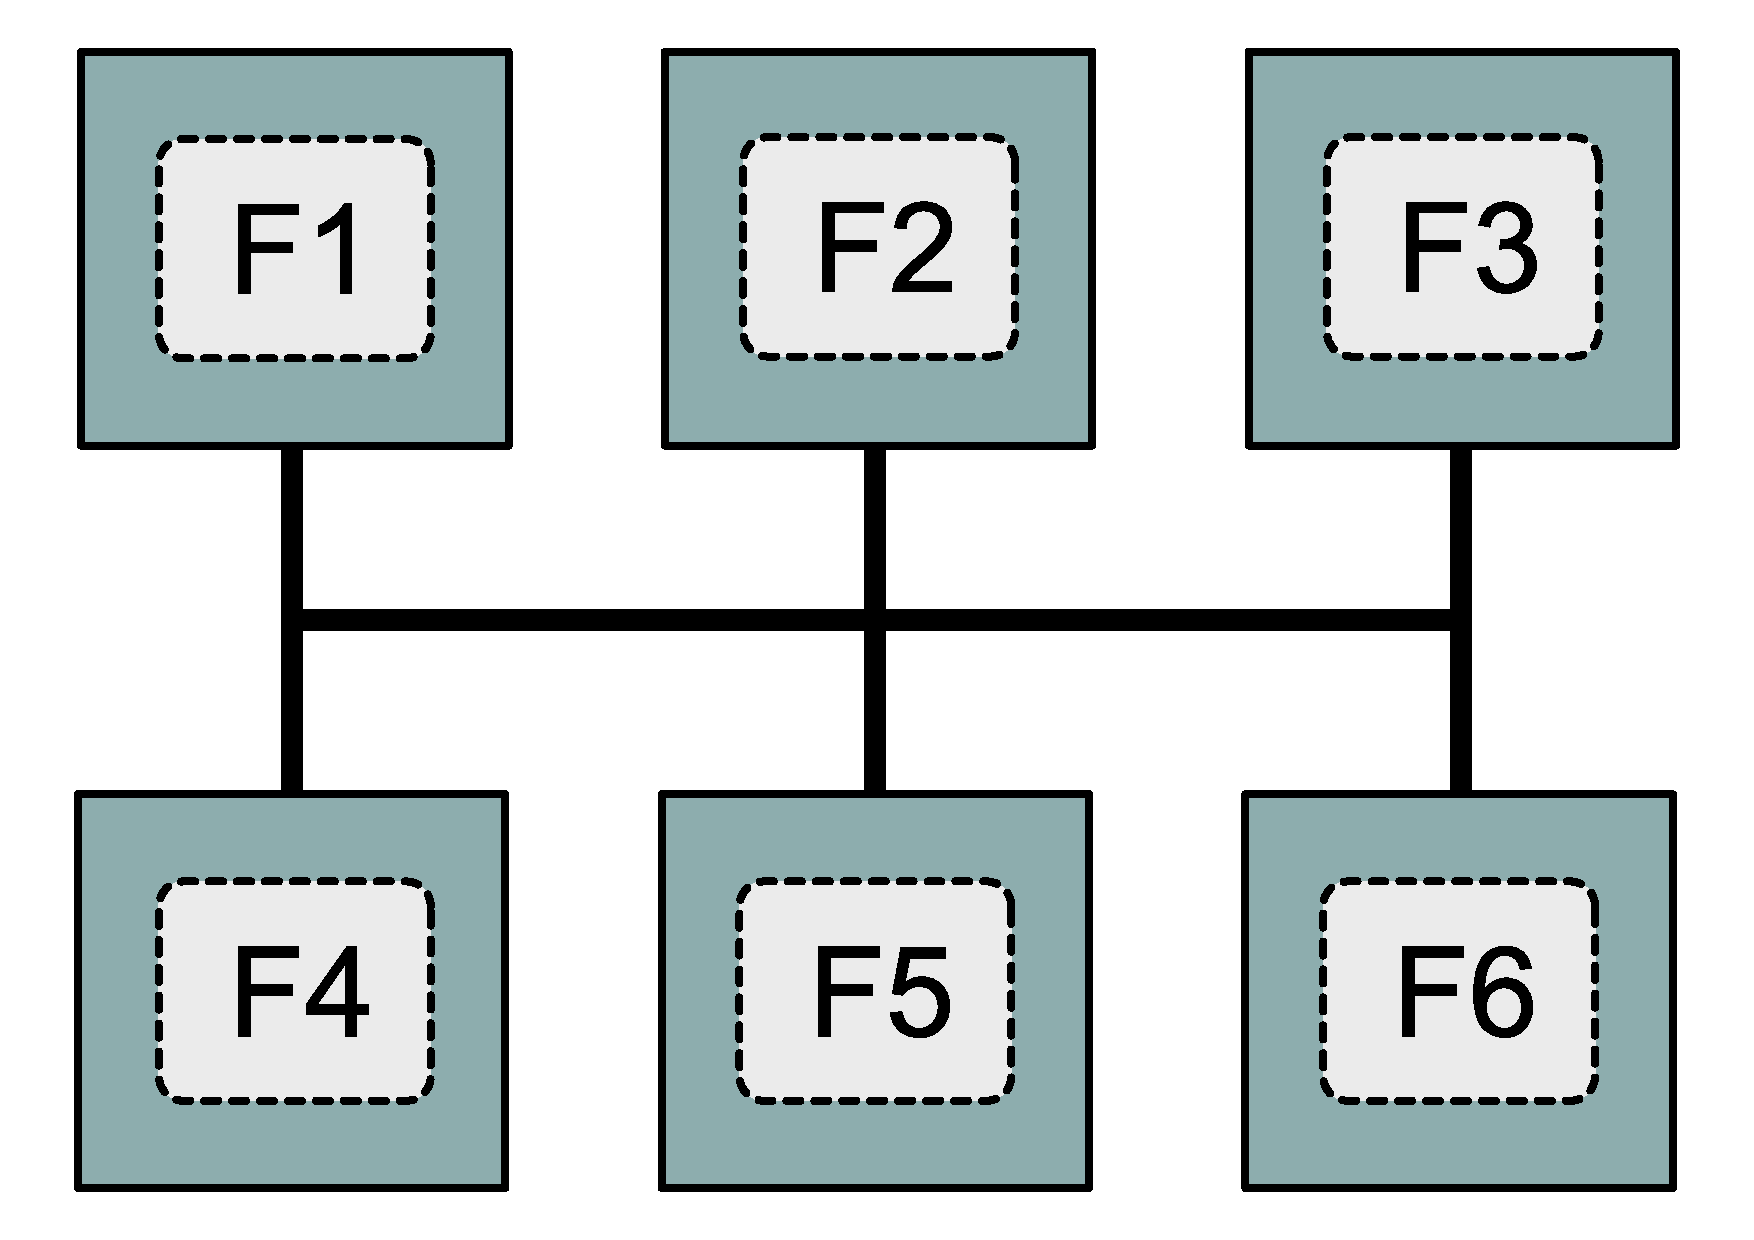
\includegraphics[width=\linewidth]{graphics/figures/federated.pdf}
		\caption{\label{fig:federe}Système fédéré}
	\end{subfigure}
	\begin{subfigure}{0,4\linewidth}
		\centering
		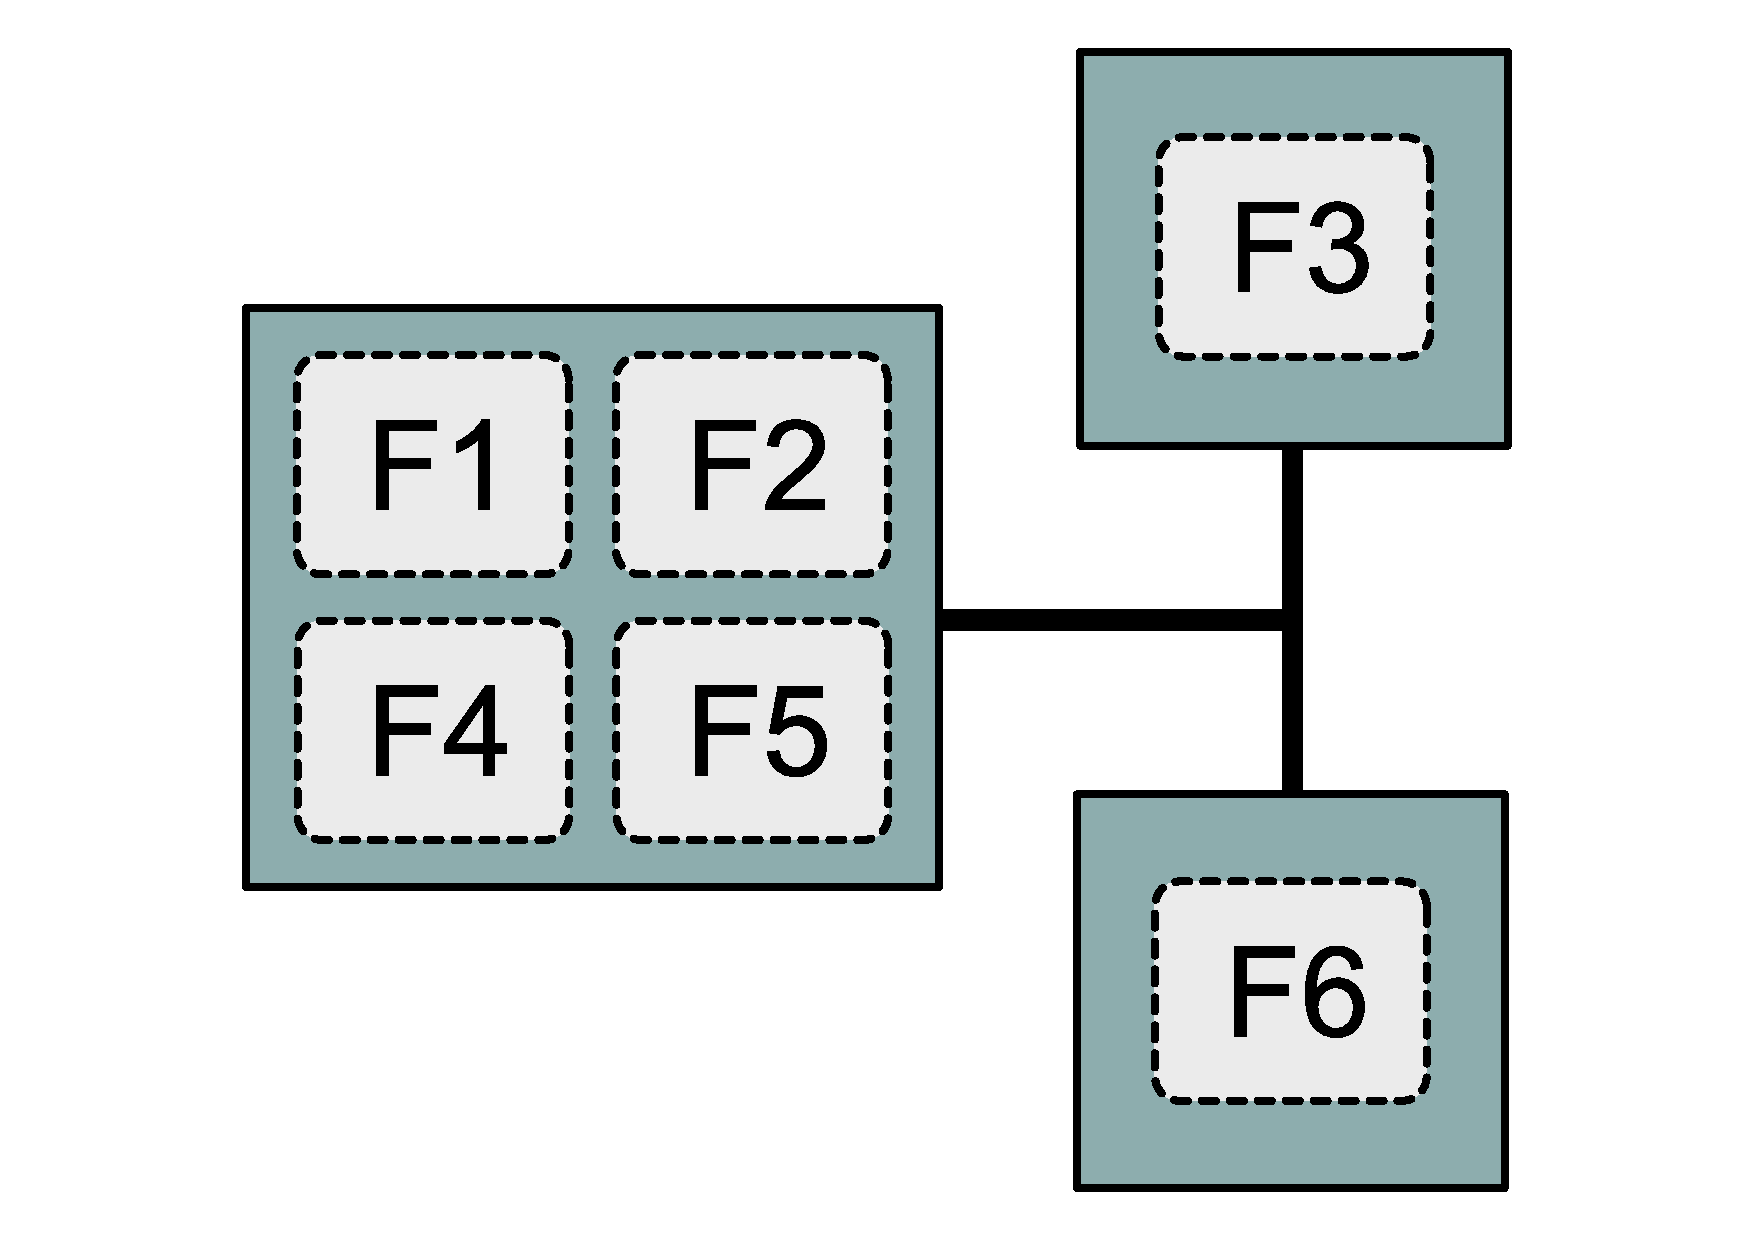
\includegraphics[width=\linewidth]{graphics/figures/integrated.pdf}
		\caption{\label{fig:integre}Système intégré}
	\end{subfigure}
	\caption{\label{fig:integre_federe}Architectures de systèmes embarqués}
\end{figure}

La montée en complexité des systèmes embarqués entraine une forte tendance à l'adoption des architectures intégrées.
C'est par exemple le cas dans l'avionique avec l'architecture \emph{IMA}~\footnote{Integrated Modular Avionics}~\cite{prisaznuk1992integrated}, utilisée, entre autres, dans l'A380 et l'A350.
Dans un système intégré, les fonctions sont autant d'\emph{applications} disposant de leur propre espace d'adressage et communiquant avec le reste du système au moyen d'une interface commune (comme ARINC 653~\cite{prisaznuk2008arinc} dans les systèmes avioniques ou encore AUTOSAR~\cite{autosar} dans l'automobile).
Un logiciel d'infrastructure (système d'exploitation ou hyperviseur) fait l'interface entre les applications et le matériel.

Le logiciel d'infrastructure est notamment en charge de maintenir l'\emph{isolation spatiale et temporelle} des applications.
L'isolation spatiale assure que deux applications ne puissent accéder à la mémoire de l'autre.
Tandis que l'isolation temporelle assure que la performance d'une application ne puisse être affectée par les autres applications du système.

\subsection{Architecture matérielle}

Nos travaux portent sur l'utilisation de cartes multi-cœurs dans les calculateurs.
Ce type de carte permet d'intégrer plus de fonctions au sein d'un même calculateur, en exécutant des fonctions en parallèle.
Parmi toute l'offre disponible, nous ciblerons des processeurs en particulier.
Il s'agit de petites cartes UMA~\footnote{Unified Memory Access} Achetée sur étagère et destinées au marché de masse.
Elles comportent un nombre restreint (entre deux et huit) de cœurs, mais chacun d'eux offre de bonnes performances.
La performance des processeurs que nous ciblons repose sur des fonctionnalités matérielles complexes (préchargement de donnée, prédiction de branchement, exécution dans le désordre, etc.), dont le fonctionnement est le plus souvent peu documenté.
Par conséquent, nous nous efforcerons de faire le moins d'hypothèses possible sur le matériel.
Des exemples processeurs de ce type cité dans la littérature sont le Cortex-A9, ou encore le PowerPC P5040.

Une hypothèse importante pour la suite de nos travaux est la présence de matériel partagé entre les cœurs.
Ce partage de matériel est à l'origine d'\emph{interférences}, sur lesquelles nous nous pencherons dans la section suivante.
Les interférences sont source de ralentissements particulièrement problématiques dans le cadre de systèmes intégrés, car l'isolation temporelle peut ne pas être respectée.
Notons que si certaines architectures partagent des ressources de calcul au niveau des cœurs (technologie HyperThread), ce ne sera pas le cas de celles que nous considérons dans nos travaux.
On fera ainsi l'hypothèse qu'un cœur ne peut exécuter au plus qu'un seul fil d'exécution.

\subsection{Architecture logicielle}

L'exploitation d'une plateforme multi-cœur peut se faire à l'aide de deux modèles de programmation, impactant l'architecture logicielle du système.
\begin{itemize}
	\item \emph{Modèle symétrique ou Symetric Multi-Processing (SMP)} Une fonction peut s'exécuter sur plusieurs cœurs à la fois.
	Une fonction est donc découpée en plusieurs composants logiciels qui correspondent à autant de fils d'exécution pouvant avoir besoin d'être synchronisée.
	Ce modèle permet à une application d'utiliser au mieux le matériel disponible, mais sa mise en œuvre peut nécessiter des adaptations des \emph{applications patrimoniales} si celles-ci ont été développées pour des systèmes mono-cœur.

	\item \emph{Modèle asymétrique ou Asymetric Multi-Processing (AMP)} Une fonction ne peut s'exécuter que sur un seul cœur à la fois.
	Ce modèle exploite le matériel en exécutant des fonctions distinctes en parallèle sur les différents cœurs.
	Par hypothèse, il n'y a pas de synchronisation entre les applications.
	Il peut néanmoins y en avoir avec le logiciel d'infrastructure.
	Ce modèle, bien que ne tirant pas parti du parallélisme au niveau d'une application, à l'avantage de ne pas demander la modification du logiciel patrimonial.
\end{itemize}

\begin{figure}[!h]
	\centering
	\begin{subfigure}[b]{0,35\linewidth}
		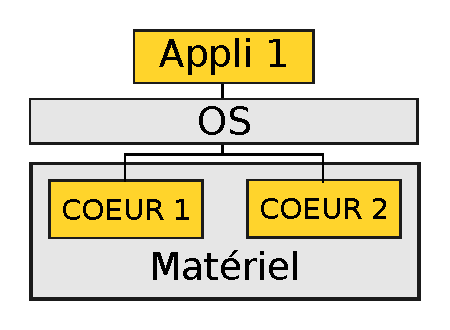
\includegraphics[width=\linewidth]{figures/smp.pdf}
		\caption{\label{fig:smp} Modèle symétrique (SMP)}
	\end{subfigure}
	\begin{subfigure}[b]{0,35\linewidth}
		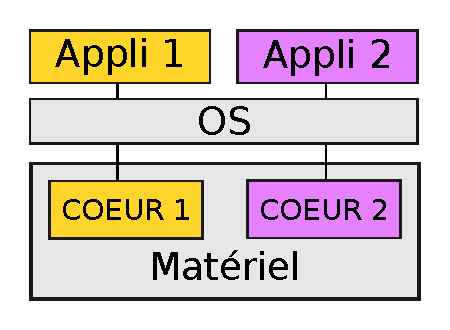
\includegraphics[width=\linewidth]{figures/amp.pdf}
		\caption{\label{fig:amp} Modèle asymétrique (AMP)}
	\end{subfigure}
	\caption{\label{fig:amp-smp} Modèles de programmation pour les systèmes multicœurs}
\end{figure}

Dans nos travaux, nous ferons l'hypothèse de fonctions implantées selon le modèle AMP. 
Ce choix est motivé par deux raisons.
Tout d'abord, les applications patrimoniales étant prépondérantes dans les systèmes embarqués, il s'agit d'un choix réaliste sur le plan industriel.
Deuxièmement, comme nos travaux portent sur l'effet des interférences dues au partage de matériel, nous souhaitons exclure autant que possible les retards résultant de l'attente causée par des synchronisations.

\subsection{Impact sur nos travaux}

Dans cette section, nous avons décrit l'architecture générale que l'on retrouve dans les systèmes embarqués complexes.
Nous avons aussi formulé un certain nombre d'hypothèses, posant un cadre de travail pour le reste de cette thèse.
Ces hypothèses sont les suivantes :
\begin{itemize}
	\item Les systèmes étudiés sont à \emph{criticité mixte}.
	Ils comprennent des applications critiques et non-critiques.
	Les applications critiques sont soumises à des contraintes temps-réels, et on ne peut pas faire d'hypothèses sur les applications non critiques.

	\item Les systèmes étudiés sont conçus selon une architecture intégrée, un calculateur est partagé par plusieurs fonctions.
	Un logiciel d'infrastructure est en charge d'assurer l'isolation spatiale et temporelle des différentes fonctions.

	\item Les calculateurs sont basés sur des processeurs multi-cœur COTS destinés au marché de masse.
	On se concentre sur des processeurs UMA disposant d'un nombre restreint de cœurs offrant chacun de bonnes performances.
	Les cœurs partagent du matériel causant ainsi des interférences temporelles.
	En conséquence, l'isolation temporelle n'est pas assurée lorsque deux applications s'exécutent en parallèle.

	\item Les fonctions du système sont supposées indépendantes les unes des autres, elles ne communiquent et ne se synchronisent donc pas.
	Elles sont de plus implantées selon un modèle asymétrique, et ne comportent donc pas de fil d'exécution s'exécutant en parallèle.
	Par conséquent, nous supposons l'absence de couplage explicite entre les cœurs, et nous concentrons donc uniquement sur l'effet des interférences.
\end{itemize}

Dans la section suivante, nous allons présenter les différents composants matériels à la source du phénomène d'interférences.

\section{Canaux d'interférences dans les systèmes multicœurs COTS}

Le matériel destiné aux applications grand public est conçu pour offrir de \emph{bonnes performances moyennes}, tout en respectant de fortes contraintes de \emph{coûts}.
Afin de réaliser ces objectifs, la conception de ce matériel s'appuie sur le partage de ressources matérielles entre les différents cœurs.
Ce partage crée un \emph{couplage implicite} des applications s'exécutant en parallèle.
En effet, l'accès concurrent aux ressources partagées par les différents cœurs est une source d'\emph{interférences}, occasionnant le plus souvent des ralentissements.
Nous pouvons distinguer deux types d'interférences:
\begin{itemize}
	\item Une application souffre d'interférences \emph{spatiales} lorsqu'une ressource est rendue indisponible par une autre application.
	Par exemple, des données en cache évincées au profit d'une autre application.

	\item Une application souffre d'interférences \emph{temporelles} lorsque son temps d'accès à une ressource est allongé au profit d'une autre application.
	Par exemple, lors de l'accès à un bus partagé.
\end{itemize}

Les ressources matérielles partagées entre les cœurs sont donc autant de \emph{canaux d'interférences} pour les applications s'y exécutant en parallèle.
Un inventaire de ces différents canaux a été dressé par Kotaba et al.~\cite{kotaba2013multicore}, que nous reprenons dans le tableau~\ref{table:canaux_interferences}.
Donc, du fait des hypothèses formulées dans la section précédente, nous ne nous préoccupons pas des canaux d'interférences suivants:
\begin{itemize}
	\item \emph{Les interférences des étages de pipelines}, car nous faisons l'hypothèse d'architectures ne disposant pas d'hyperthreading.
	\item \emph{Les interférences sur les périphériques et les unités logiques}, car l'accès à ces ressources se fait à travers le logiciel d'infrastructure.
	Il ne s'agit donc pas à proprement parler d'une ressource accédée implicitement.
	\item \emph{Les interférences dues aux protocoles de cohérences de données}, car nous faisons l'hypothèse d'un modèle de programmation asymétrique (AMP).
	Les données d'une application ne peuvent donc à priori pas être invalidées.
\end{itemize}

\begin{savenotes}
\begin{table}[!ht]
	\centering
	\resizebox{\linewidth}{!}{
		\begin{tabular}{r c l}
\toprule
Canal & Type\footnotemark & Interférence\\
\midrule
Bus système 	& T & contention causée par les coeurs \\
				& T & Contention causées par les périphériques \\
				& T & Contention causées par les procoles de \\
				&   & cohérences \\ 

\midrule

Passerelles 	 & \multirow{2}{*}{T} & \multirow{2}{*}{Contentions causées par les autres bus} \\
d'interconnexion & & \\

\midrule
Mémoire principale & S & Fermetures de pages par d'autre applications \\
				   & T & Réordonancements de requêtes d'accès \\

\midrule
Caches partagés & S & Éviction de donnés par d'autres applications \\
				& T & Accès concurrent au cache \\
				& S & Invalidation de données par les protocoles de \\
				&   & cohérences \\

\midrule
Caches locaux   & S & Invalidation de données par les protocoles de \\
				&   & cohérences \\

\midrule
TLB 			& S & Invalidation d'entrées par les protocoles de \\ 
				&   & cohérences \\

\midrule
Périphériques & T & Contention entre applications \\
			  & T & Routage des interruptions \\

\midrule
Étages des pipeline & T & Contention dans les architectures hyperthreadés \\

\midrule
Unité logiques 			  & \multirow{2}{*}{T} & \multirow{2}{*}{Contention entre applications.} \\
(Coprocesseurs, GPU, ...) & & \\

\bottomrule
\footnotetext{S : spatial T : temporel}
\end{tabular}
	}
	\caption{\label{table:canaux_interferences}Interférences rencontrées dans les cibles multicœurs (source Kotaba et al.~\cite{kotaba2013multicore})}
\end{table}
\end{savenotes}

\subsection{Impact sur nos travaux}

Les interférences sont une source de ralentissements dans les processeurs multi-cœurs COTS.
Elles peuvent être induites par des arbitrages d'accès (interférences temporelles) ou bien par le vol de ressources entre les différents cœurs (interférences spatiales).
Elles peuvent se produire dans différents composants que nous désignons par le terme canal d'interférences.
Parmi les canaux d'interférences recensés sur le matériel actuel, notre regard se porte sur ceux du système mémoire.
Dans la section suivante, nous allons expliquer plus en détail les différentes interférences pouvant affecter ce dernier.

\section{Système mémoire}

Au fil des années, le système mémoire est devenu un élément de plus en plus critique dans la performance des processeurs.
Une explication est donnée par la figure~\ref{fig:gap_memoire_processeur} illustrant l'évolution dans le temps de la performance des processeurs et de celles du temps d'accès à la mémoire.
On peut y constater qu'entre 1980 et 2015, les processeurs sont devenus 10 000 fois plus rapides, tandis que le temps d'accès à la mémoire n'a été divisé que par 10.
Dans ces conditions, la dégradation des performances du système mémoire par les interférences va avoir un impact important sur la performance globale du matériel.
C'est pour cette raison que la mémoire est au cœur des préoccupations soulevées par les interférences.

\begin{figure}[!h]
	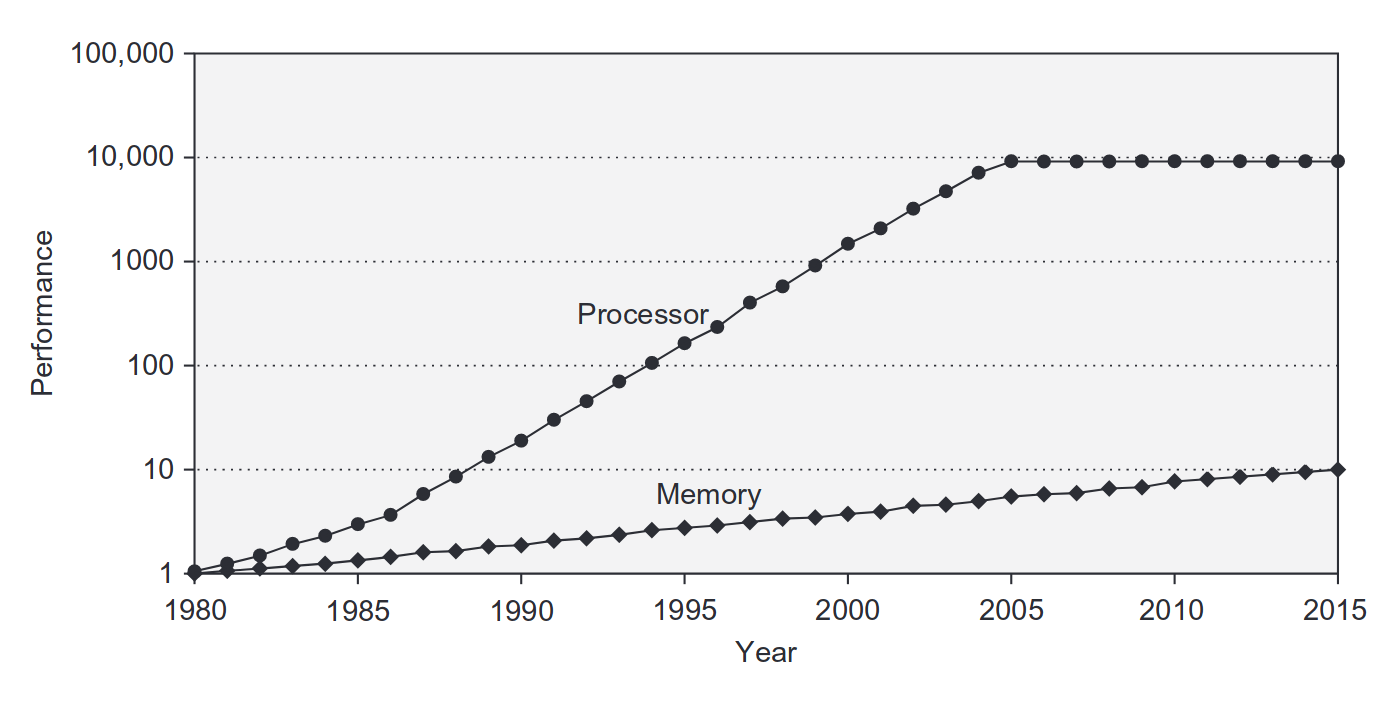
\includegraphics[width=\textwidth]{graphics/figures/gap_memory_processor.png}
	\caption{\label{fig:gap_memoire_processeur}Évolution des performances respectives de la mémoire et des processeurs, normalisés par leur niveau en 1980 (Source de l'illustration Hennessy et Patterson~\cite{hennessy2011computer}).}
\end{figure}

Dans le reste de cette section, nous présenterons le système mémoire et les différentes interférences pouvant l'affecter.
Nous commencerons par décrire les caractéristiques des mémoires actuelles et comment elles sont organisées.
Nous nous pencherons ensuite sur le fonctionnement de la mémoire principale, puis sur celle des caches.

\subsection{Caractéristiques des mémoires et organisation}

La \emph{mémoire vive ou Random Access Memory (RAM)} désigne la mémoire dans laquelle les données peuvent être stockées et effacées.
On peut la représenter comme un ensemble de \emph{cellules} connectées entre elles, chacune stockant un \emph{bit} de donnée.
Il y a deux grandes familles de technologie pour les cellules de mémoire vive: les cellules de \emph{mémoire statiques ou Static Random Access Memory (SRAM)} et les cellules de \emph{mémoire dynamiques ou Dynamic Random Access Memory (DRAM)}.

La mémoire statique fonctionne sur le principe d'une bascule RS.
Une bascule RS est une porte logique avec deux entrées $R$ et $S$ et deux sorties $Q$ et $\bar{Q}$.
Si $S=1$ et $R=0$, alors $Q=1$.
Si $S=0$ et $R=1$, alors $Q=0$.
Lorsque $R$ et $S$ valent 0 alors la valeur de $Q$ est inchangée.
$R$ et $S$ ne peuvent pas valoir 1 simultanément.
On peut donc utiliser une bascule RS pour stocker un bit.
Lire une mémoire statique consiste simplement à mesurer la sortie de la bascule, la rendant extrêmement rapide.
La contrepartie est la faible densité d'intégration que permet cette technologie.
En effet, la SRAM est le plus souvent de type 6T (illustré sur la figure~\ref{fig:sram_cell}) qui utilise 6 transistors, ce qui s'avère extrêmement coûteux.

La mémoire dynamique (DRAM) stocke la valeur d'un bit dans un condensateur gardé par un transistor.
Si le condensateur est chargé le bit vaut 1, sinon il vaut 0.
La mémoire est lue en fermant le transistor, et en vérifiant si le transistor était chargé ou non.
Cette technologie permet une grande densité d'intégration, vu que seulement un transistor et un condensateur sont requis.
Elle présente néanmoins trois inconvénients:
\begin{enumerate}
	\item Les latences de lecture et d'écritures sont importantes, du fait qu'elles sont contraintes par le temps de charge et décharge du condensateur.
	\item Vu que le condensateur doit être déchargé pour déterminer l'état de la cellule, la lecture est destructive.
	\item Les condensateurs se déchargent avec le temps. 
	L'état des cellules doit donc être rafraichi périodiquement pour éviter de perdre des données.
	Cela consiste simplement à lire puis réécrire les données.
\end{enumerate}

\begin{figure}[!h]
	\centering
	\begin{subfigure}[b]{0,5\textwidth}
		\centering
		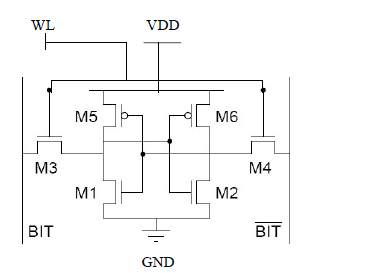
\includegraphics[width=\linewidth]{graphics/figures/6T-SRAM-Cell-III-PROPOSED-EIGHT-TRANSISTOR-8T-SRAM-CELL-In-this-proposed-SRAM-Dual}
		\caption{\label{fig:sram_cell} Cellule de SRAM 6T}
	\end{subfigure}
	\begin{subfigure}[b]{0,3\textwidth}
		\centering
		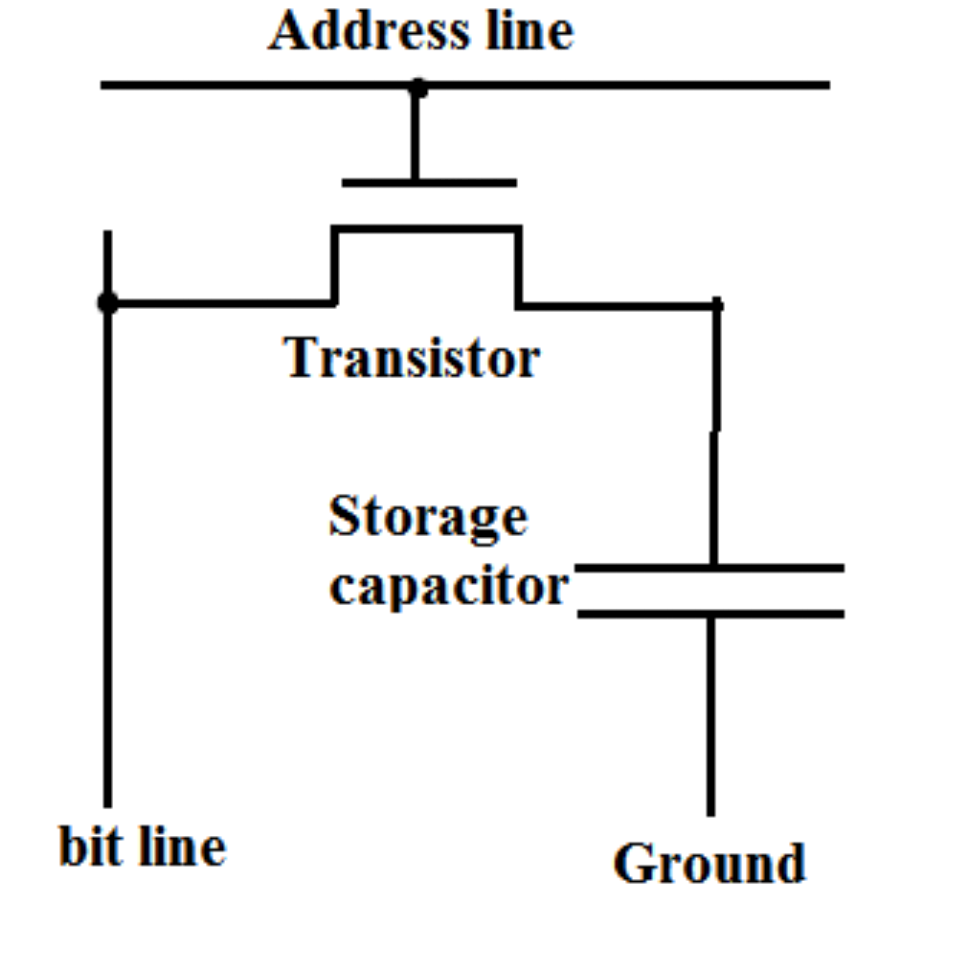
\includegraphics[width=0.5\linewidth]{graphics/figures/dram_cell}
		\caption{\label{fig:sram_cell} Cellule de DRAM}
	\end{subfigure}
	\caption{\label{fig:memoire_statique_dynamique} Circuit des différents types de cellules mémoires actuellement disponible.}
\end{figure}

Les caractéristiques de la DRAM et de la SRAM font qu'à coût équivalent, une mémoire est, à l'heure actuelle,  soit rapide soit de grande capacité.
La surface étant l'un des principaux facteurs de coûts d'un composant électronique.
Afin de donner l'illusion d'une mémoire à la fois rapide et de grande capacité, les systèmes mémoires sont organisés hiérarchiquement; chaque niveau de cette hiérarchie étant à la fois plus éloigné du processeur et comportant une mémoire plus grosse et plus lente que le niveau inférieur.
Ce type d'architecture est très répandu, il s'agit d'ailleurs d'une idée assez ancienne, remontant au fondement des premiers ordinateurs~\cite{von1946preliminary}.
La hiérarchie mémoire type rencontrée dans le matériel utilisé dans les terminaux mobiles est illustré dans la figure~\ref{fig:hierarchie_memoire}.

\begin{figure}[!h]
	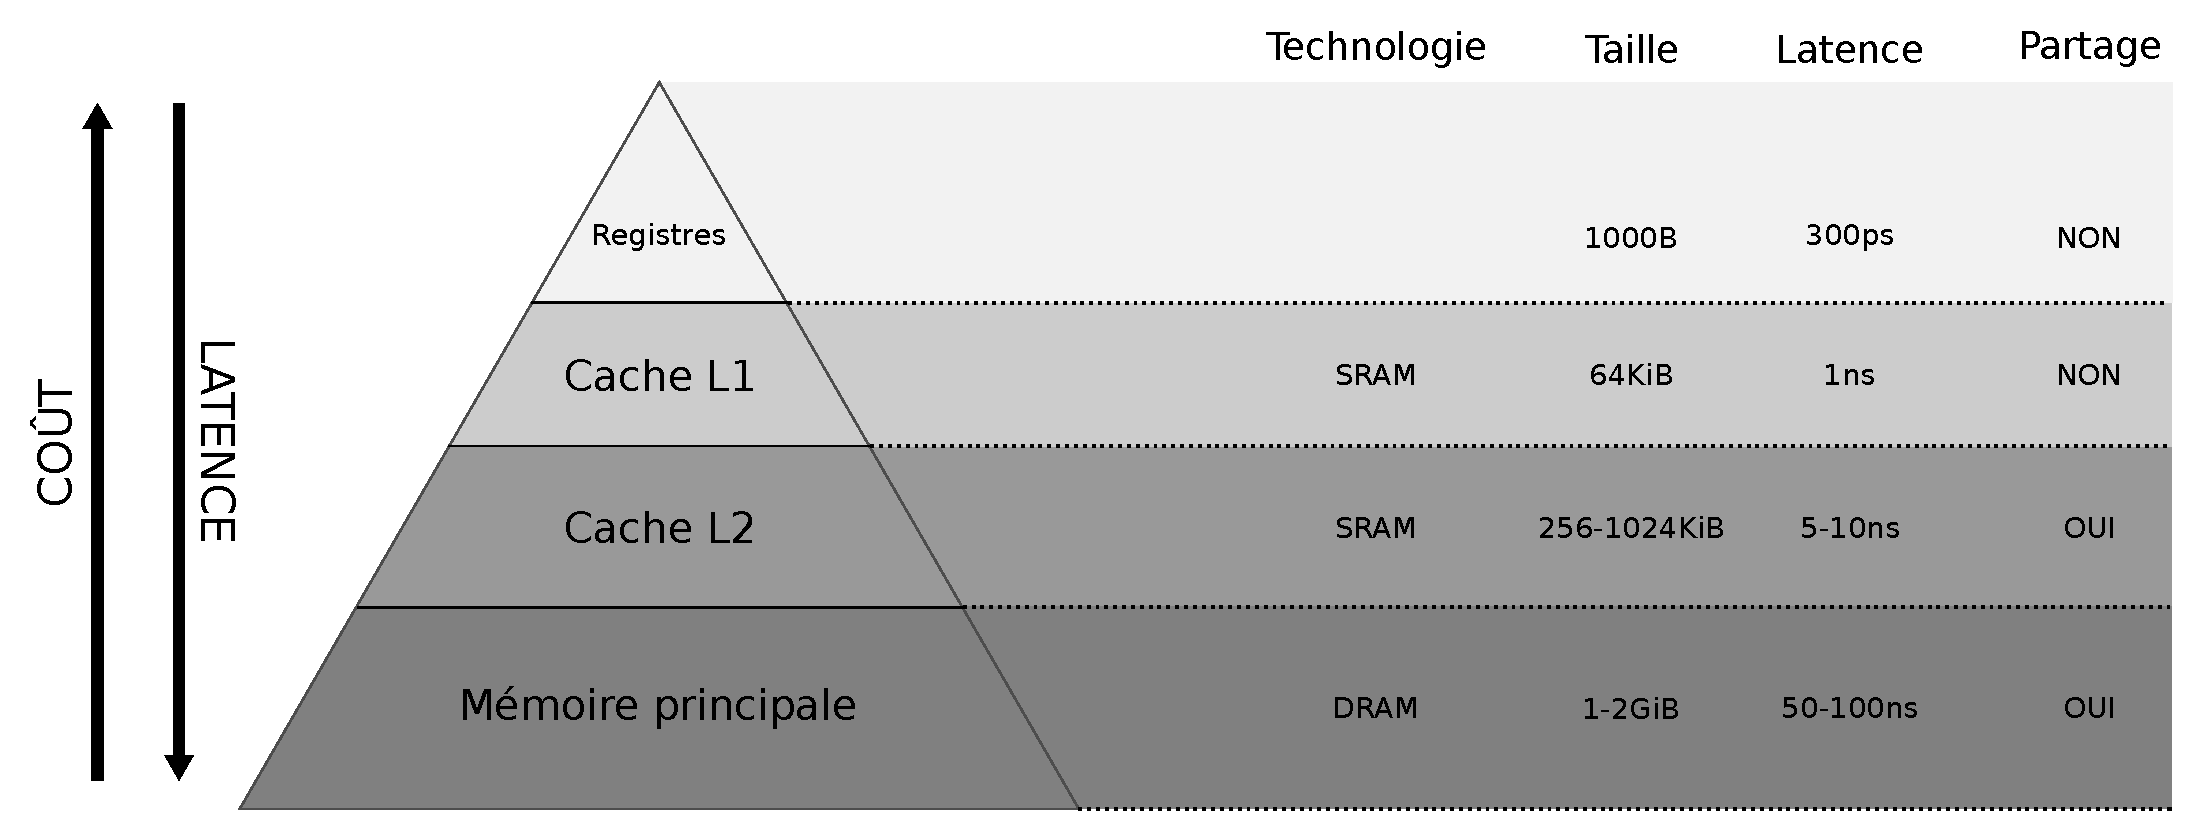
\includegraphics[width=\linewidth]{graphics/figures/hierarchie.pdf}
	\caption{\label{fig:hierarchie_memoire} Hiérarchie mémoire couramment rencontrée dans les terminaux mobiles}.
\end{figure}

Le niveau le plus bas de la hiérarchie mémoire est occupé par les registres, utilisés par le processeur pour le stockage des opérandes et des résultats intermédiaires.
Le niveau le plus haut est occupé par la mémoire principale basée sur la technologie DRAM.
Les niveaux intermédiaires sont occupés par les \emph{caches}, destinés à accélérer l'accès à la mémoire principale en stockant les données accédées récemment dans de la SRAM.
Cette architecture est conçue pour exploiter deux caractéristiques du comportement d'accès à la mémoire couramment observé dans les programmes: la localité spatiale~\cite{liptay1968structural} et la localité temporelle~\cite{wilkes1965slave}.
La propriété de localité spatiale exprime une forte probabilité que lorsqu'une donnée est accédée, les données voisines sont accédées dans un futur proche.
Tandis que la propriété de localité temporelle exprime une forte probabilité qu'une donnée accédée récemment le soit de nouveau dans un futur proche.
Dans les processeurs multicœurs, les niveaux supérieurs de cette hiérarchie sont généralement partagés, faisant des caches et de la mémoire principale d'éventuels canaux d'interférences.
Nous allons maintenant détailler le fonctionnement et l'impact des interférences sur ces deux composants.

\subsection{Mémoire principale}

La mémoire principale est implantée par des cellules de DRAM afin d'offrir une grande capacité de stockage.
L'utilisation de ce type de cellules apporte un certain nombre de contraintes, qui impose une organisation particulière que nous allons maintenant détailler.

\subsubsection{Organisation}

La mémoire principale est composée de modules (Dual Inline Memory Module ou DIMM) et de contrôleurs mémoires.
Un ensemble de modules mémoire est associé à un contrôleur mémoire par le biais d'un \emph{canal de communication ou channel}.
Ce canal est constitué de trois bus: un \emph{bus de commande}, un \emph{bus d'adresse}, et un \emph{bus de données}.
Le contrôleur reçoit des requêtes d'accès mémoires qu'ils décomposent en une série de commandes.
Les bus de commandes, d'adresses et de données sont alors utilisés respectivement pour transférer les commandes, les adresses de destination et les données lues ou écrites.

Un module mémoire comprend plusieurs \emph{puces mémoires} qui sont regroupées en ranks.
Une requête mémoire est émise à destination d'un rank en particulier, les puces qui le composent sont alors activées.
Les puces constituant un rank partagent le bus de commandes et d'adresse, mais occupent chacune une portion du bus de donnée.
Cela signifie que les données sont transférées en parallèle à partir de toutes les puces du rank, permettant ainsi de compenser la latence de la DRAM par une bande passante plus élevée.

Chaque puce est constitué de plusieurs \emph{bancs mémoires} ou plus rarement \emph{pages} (à ne pas confondre avec les pages de mémoire virtuelle).
Un banc mémoire comprend une matrice de cellules DRAM organisé en ligne et en colonne, plus une ligne supplémentaire appelée \emph{row buffer}.
Lorsque une donnée est accédée dans un banc mémoire, toute la ligne à laquelle elle appartient est chargée dans le row buffer.
Il y a deux raisons à cela.
D'une part, cela permet de gérer le fait que lire une cellule de DRAM détruit son contenu.
D'autre part, cela permet d'accélérer l'accès aux données présentes sur la même ligne.
Si la ligne à laquelle appartient une donnée auquelle on souhaite accéder n'est pas chargée, il y a alors \emph{un défaut de ligne ou row miss}.
Il faut alors écrire la ligne présente dans le row buffer (qu'elle ait été modifiée ou non) avant de charger la ligne désirée.

\begin{figure}
	\centering
	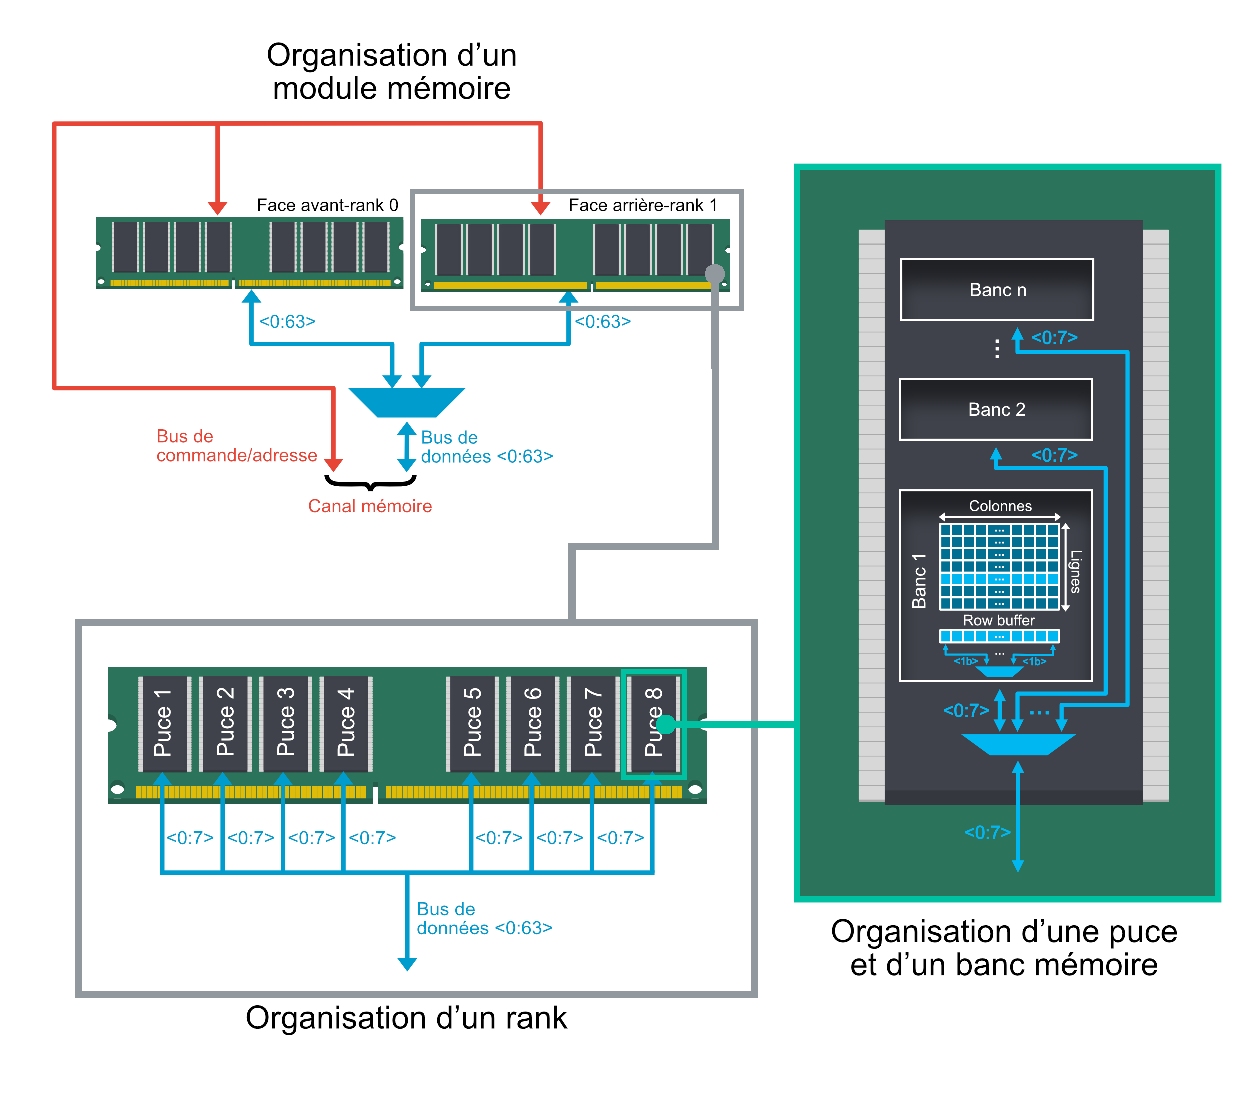
\includegraphics[width=\linewidth]{graphics/figures/orga-dram.pdf}
	\caption{\label{fig:dram_organization}Organisation de la mémoire principale}
\end{figure}
% \begin{figure}
% 	\centering
% 	\begin{tabular}{c c}
% 		\begin{subfigure}[t]{0,5\linewidth}
% 			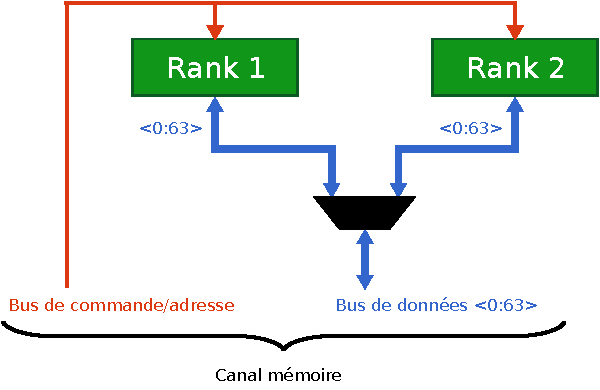
\includegraphics[width=0.75\linewidth]{graphics/figures/dimm2.pdf}
% 			\caption{\label{fig:dimm}Modules mémoires}
% 		\end{subfigure} & 
	
% 		\begin{subfigure}[t]{0,5\linewidth}
% 			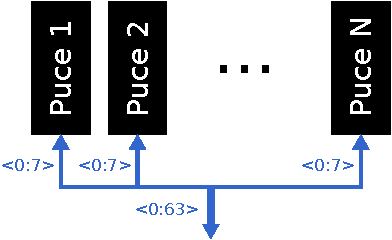
\includegraphics[width=0.75\linewidth]{graphics/figures/rank3.pdf}
% 			\caption{\label{fig:rank}Rank}
% 		\end{subfigure} \\
% 		& \\
% 		\begin{subfigure}[t]{0,3\linewidth}
% 			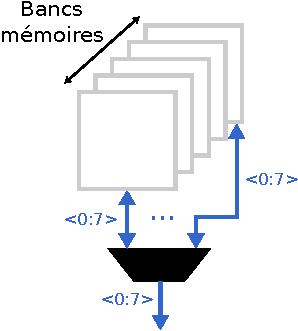
\includegraphics[width=\linewidth]{graphics/figures/chip2.pdf}
% 			\caption{\label{fig:rank}Puce mémoire}
% 		\end{subfigure} & 
		
% 		\begin{subfigure}[t]{0,3\linewidth}
% 			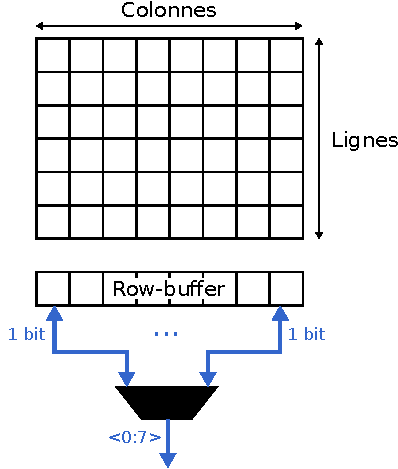
\includegraphics[width=\linewidth]{graphics/figures/bank2.pdf}
% 			\caption{\label{fig:bank}Banc mémoire} 
% 		\end{subfigure} \\
% 	\end{tabular}
% 	\caption{\label{fig:dram_organization}Organisation de la mémoire principale}
% \end{figure}

\subsubsection{Contrôleur DRAM}

Le contrôleur DRAM est en charge de traiter les différentes requêtes d'accès à la DRAM, tout en maintenant cette dernière dans un état de fonctionnement correct.
Il gère entre autres les différentes contraintes temporelles, dont le rafraichissement des cellules.
Le contrôleur reçoit des requêtes de lectures et d'écritures qu'il traduit en un ensemble de commandes agissant sur les bancs mémoires.
Plusieurs commandes sont définies par les JEDEC~\cite{specification2010jesd79}(l'organisation gérant les normes concernant la mémoire dynamique), parmi lesquels nous citerons les suivantes:

\begin{itemize}
	\item \texttt{ACT} charge une ligne dans le row buffer.
	\item \texttt{PRE} Vide le contenu du row buffer dans les cellules mémoire correspondantes.
	\item \texttt{READ} Lecture depuis le row buffer
	\item \texttt{WRITE} Écriture dans le row buffer
	\item \texttt{REF} Rafraichissement d'une ligne.
	Il s'agit de la combinaison d'une commande \texttt{ACT} et \texttt{PRE}.
	Cela a pour conséquence de vider le row buffer.
\end{itemize}

Les row buffers jouent un rôle essentiel dans la performance dans le DRAM.
Ils peuvent être gérés suivant deux politiques.
\begin{itemize}
	\item \emph{La politique open-row} Une ligne chargée dans un row buffer le reste jusqu'a son éviction.
	Cette stratégie est optimale pour les accès séquentiels.
	Par contre, le coût des défauts de lignes est élevé, étant donné qu'il faut écrire le contenu du row buffer avant de charger la nouvelle ligne.

	\item \emph{La politique close-row} La ligne est close après chaque accès.
	Cette politique offre un meilleur pire cas en évitant les conflits sur les row buffers, mais dégrade les performances en moyenne.
\end{itemize}

Le contrôleur mémoire est également en charge de maximiser les performances d'accès à la DRAM.
Pour cela, il réordonnance les requêtes d'accès afin de maximiser le débit de requêtes traitées et la bande passante de la mémoire principale.
La politique le plus couramment utilisée est \emph{Premier Prêt/Premier Arrivé Premier Servi ou FR/FCFS}.
Dans cette politique, les requêtes sont traitées dans l'ordre d'arrivée, mais une priorité est donnée à celle qui sont \emph{prête à être traitées}.
En pratique, une requête est prête à être traitée si la ligne correspondante est chargée, et si le bus de donnée est dans le bon sens (lecture ou écriture).
Le contrôleur optimise donc la bande passante globale aux dépens de l'équité des requêtes.

\begin{figure}[!h]
	\centering
	\begin{tabular} {c c}
		\begin{subfigure}[t]{0,4\linewidth}
			\centering
			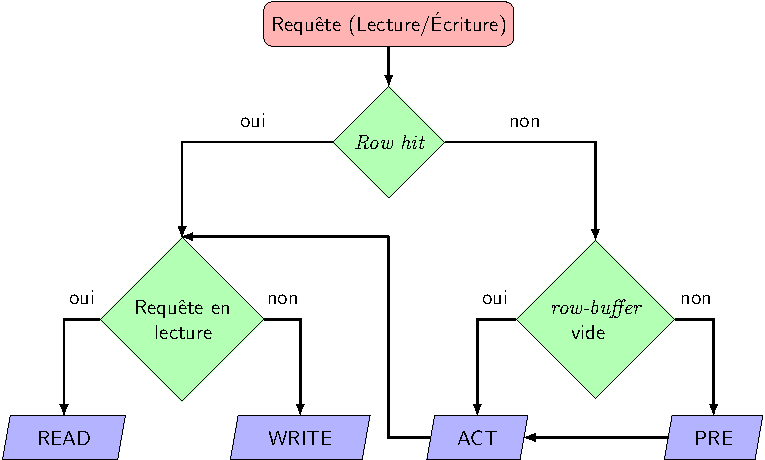
\includegraphics[width=0.8\linewidth]{graphics/figures/open_row_policy_algo2.pdf}
			\caption{\label{fig:open_row_algo}Algorithme de la politique \emph{open-row}}
		\end{subfigure} & 
		
		\begin{subfigure}[t]{0,5\linewidth}
			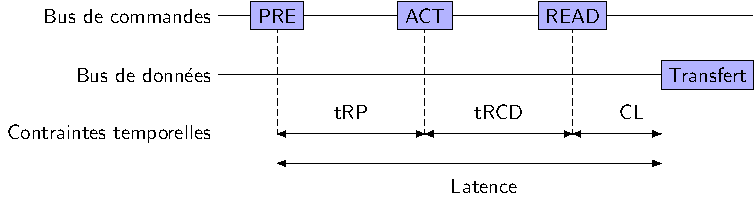
\includegraphics[width=\linewidth]{graphics/figures/open_row_policy_wcet2.pdf}
			\caption{\label{fig:open_row_wcet}Pire cas de la politique \emph{open-row}}
		\end{subfigure} \\
		& \\
		\begin{subfigure}[t]{0,3\linewidth}
			\centering
			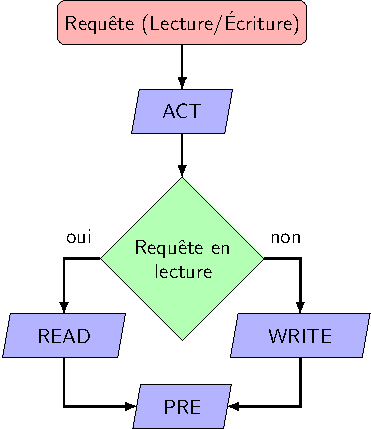
\includegraphics[width=0.6\linewidth]{graphics/figures/close_row_policy_algo2.pdf}
			\caption{\label{fig:closed_row_algo}Algorithme de la politique \emph{close-row}}
		\end{subfigure} &
		
		\begin{subfigure}[t]{0,5\linewidth}
			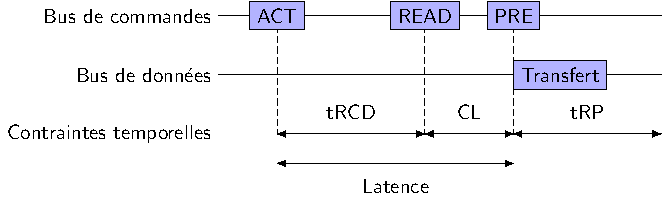
\includegraphics[width=\linewidth]{graphics/figures/close_row_policy_wcet2.pdf}
			\caption{\label{fig:closed_row_algo}Pire cas de la politique \emph{close row}}
		\end{subfigure} \\
	\end{tabular}

	\caption{\label{open_close_row}Algorithmes et pire cas des politiques de gestion de row buffer}
\end{figure}

\subsubsection{Mémoire principale et interférences}

La mémoire principale est un canal d'interférences spatiales et temporelles pour les différents cœurs qui l'utilisent.

Deux types de conflits peuvent survenir.
Les \emph{conflits de bancs} surviennent lorsque plusieurs cœurs tentent d'accéder au même banc mémoire simultanément.
Ce type de conflit est une interférence temporelle: il cause une séquentialisation des commandes.
Les \emph{conflits de lignes} surviennent lorsque deux commandes accèdent à deux lignes différentes sur le même banc, entrainant ainsi des rechargements de row buffer.
Il s'agit ici d'une interférence spatiale affectant la disponibilité des row buffers.
Ce type de conflits peut techniquement être évité en utilisant la politique close-row. 
Mais en pratique, c'est la politique open-row qui est employée, vu qu'elle permet d'atteindre de meilleures performances en moyenne.

La politique de réordonnancement de requête est une autre source d'interférence temporelle.
La politique FR/FCFS donne en effet la priorité aux requêtes d'accès pouvant être traitée immédiatement.
En conséquence, un cœur utilisant la DRAM efficacement, c'est-à-dire jouissant d'une bonne localité spatiale et temporelle, sera plus prioritaire qu'un cœur avec une utilisation moins efficace.
On peut en conclure que l'iniquité de cette politique rend plus sensibles aux interférences sur la mémoire principale les applications l'utilisant de façon non optimale.

% \begin{keypoints}
% 	\item Les caches jouent un rôle majeur dans la performance des processeurs modernes en masquant la latence d'accès à la mémoire.
% 	\item Les caches partagées constituent un canal d'interférences aussi bien spatiales que temporelles.
% \end{keypoints}

\subsection{Caches}

Les caches ont pour but de réduire la latence moyenne d'accès à la mémoire.
Pour cela, ils stockent un sous-ensemble des données présentes en mémoire dans une mémoire SRAM, qui est donc très rapide, mais de taille limitée.
En stockant les données accédées récemment, ils permettent de considérablement améliorer les performances des programmes présentant une bonne localité spatiale et temporelle.
En effet, comme on peut le constater dans la figure~\ref{fig:hierarchie_memoire}, la latence d'accès à la mémoire principale peut atteindre l'ordre de la centaine de nanosecondes contre une nanoseconde pour un accès au cache de niveau un.
Les caches sont donc un élément crucial pour la performance des processeurs modernes.

\subsubsection{Accès}

L'accès au cache est complètement transparent pour le programmeur.
Lorsqu'une donnée est accédée, le cache de plus bas niveau est d'abord interrogé sur sa présence.
Si la donnée est présente dans le cache, elle est alors accédée en lecture ou écriture depuis celui-ci.
Dans le cas contraire, la donnée doit alors être chargée depuis le niveau suivant de la hiérarchie mémoire, on parle alors de \emph{défaut de cache ou cache miss}.
Le niveau suivant de la hiérarchie mémoire peut alors être directement la mémoire principale, ou bien un autre cache.
Nous pouvons distinguer quatre types de défauts de caches:

\begin{itemize}
	\item \emph{Défauts obligatoires} La donnée est chargée pour la première fois.
	\item \emph{Défauts capacitifs} Le cache est plein, la donnée doit alors être chargée aux dépens d'une autre.
	\item \emph{Défauts conflictuels} deux données distinctes partagent le même emplacement de cache et s'évincent mutuellement.
	\item \emph{Défauts de cohérence} La donnée a été invalidée par un protocole de cohérence.
\end{itemize}

\subsubsection{Organisation}

Un cache est divisé en \emph{blocs} appelés \emph{lignes}.
Une ligne de cache comprend plusieurs mots mémoires (généralement huit).
Les transferts de données se font à la granularité du mot mémoire vers le processeur, et à la granularité de la ligne de cache vers les autres niveaux de la hiérarchie mémoire.
Des métadonnées sont associées à chaque ligne de cache, leur nature exacte pouvant varier légèrement d'un type de cache à l'autre.

Le placement des données dans le cache se fait au moyen de l'adresse de la donnée accédée.
Cette dernière contient trois informations essentielles: 
\begin{itemize}
	\item \emph{L'index} désigne un sous-ensemble de lignes de caches pouvant accueillir la donnée.
	\item \emph{L'offset} désigne la position d'un octet dans la ligne de cache.
	\item \emph{Le tag} permet de déterminer l'adresse de la donnée présente dans une ligne.
\end{itemize}

La position des bits encodant cette information est décrite dans la figure~\ref{fig:addresse_cache}.
Le découpage choisi n'est pas anodin.
Il associe aux lignes adjacentes en mémoire des index adjacents dans le cache, prévenant ainsi des défauts conflictuels pour les applications jouissant d'une bonne localité spatiale.

\begin{figure}[!h]
	\centering
	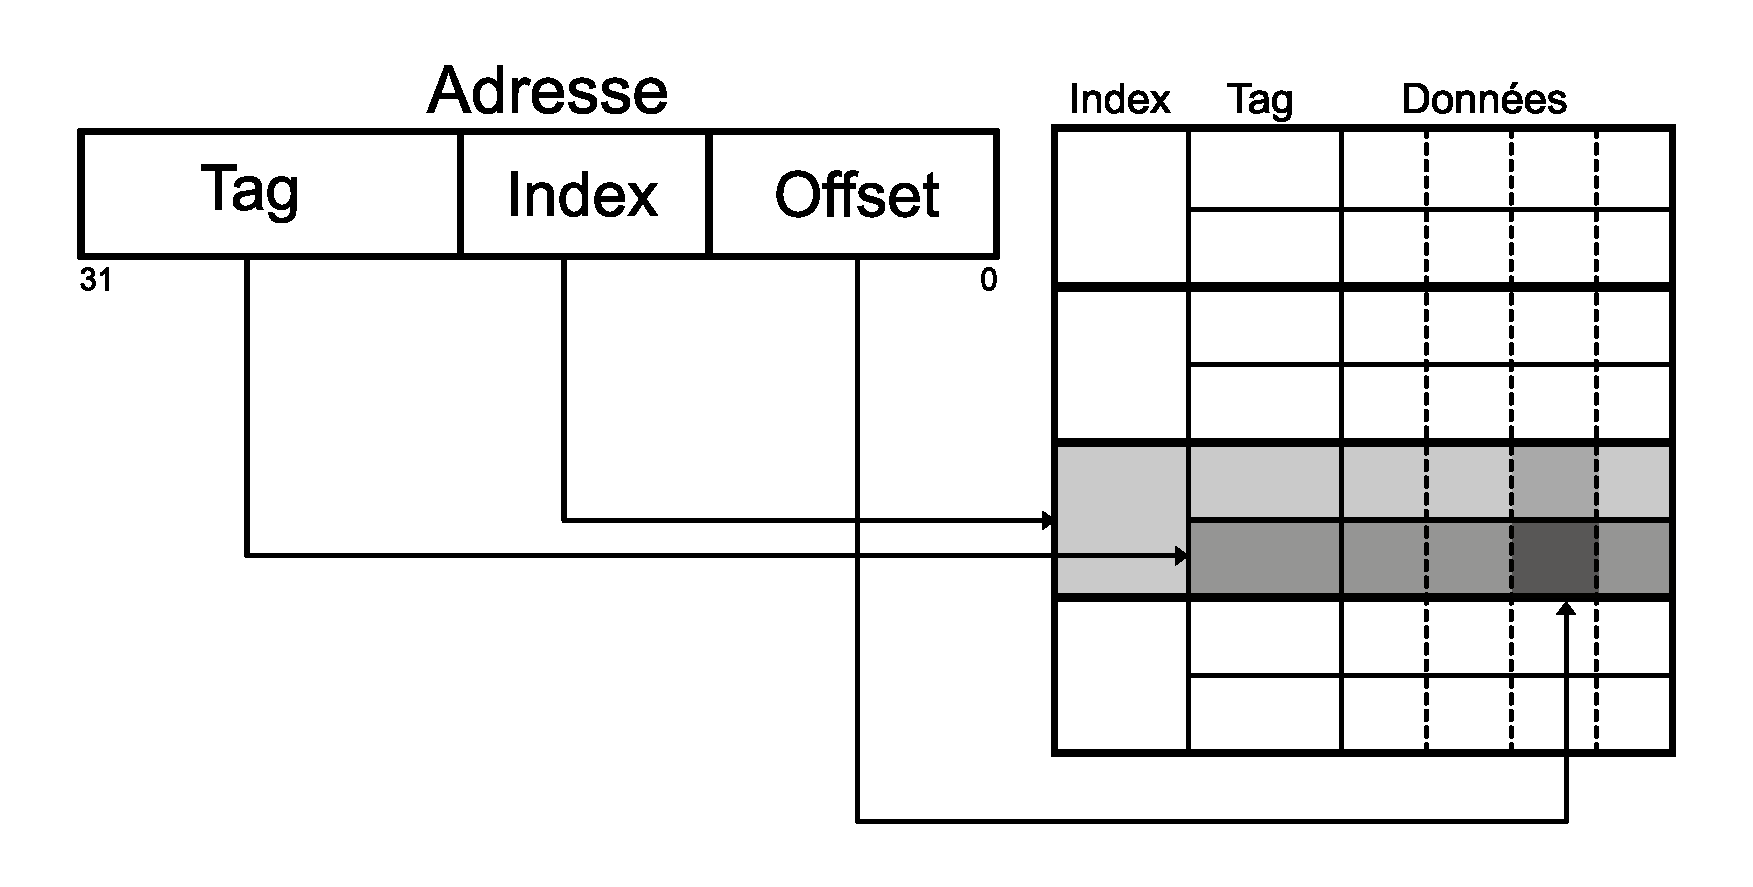
\includegraphics[width=0.9\linewidth]{graphics/figures/cache-adresse.pdf}
	\caption{\label{fig:addresse_cache}Correspondance entre les bits d'adresses et le placement des données dans un cache}
\end{figure}

On peut utiliser aussi bien l'adresse virtuelle que l'adresse physique pour tagger et indexer le cache.
On rencontre trois cas:
\begin{itemize}
	\item \emph{Cache Virtuellement Indexé et Virtuellement Taggé (VIVT)}
	Seule l'adresse virtuelle est utilisée pour interroger le cache.
	Cette méthode a l'avantage de la rapidité, vu qu'elle ne nécessite pas de traduire l'adresse.
	Elle pose néanmoins le problème des homonymes, deux mêmes adresses virtuelles pouvant désigner deux emplacements physiques différents.
	Ce problème a d'autant plus de chance de survenir dans le cas où le cache est partagé.
	Si des solutions à ce problème existent, elles se révèlent incompatibles avec les protocoles de cohérences de caches classiques~\cite{Kaxiras:2013:NPE:2485922.2485968}.

	\item \emph{Cache Physiquement Indexé et Physiquement Taggé (PIPT)}
	Seule l'adresse physique est utilisée.
	Cette méthode permet d'éviter le problème des homonymes, mais présente l'inconvénient de la lenteur, une traduction de l'adresse étant nécessaire pour interroger le cache.

	\item \emph{Cache Virtuellement Indexé et Physiquement Taggé (VIPT)}
	Cette approche vise à réduire le temps d'accès au cache en accédant à la ligne à tester pendant la traduction de l'adresse.
	L'utilisation de l'adresse physique permet d'éviter les problèmes d'homonymies.
	Pour cela, il faut néanmoins qu'il n'y ait aucun bit d'index ne soit traduit, ce qui limite cette approche aux caches de petite taille.
\end{itemize}

\subsubsection{Politiques de correspondance}

La politique de correspondance d'un cache définit quelle ligne peut être occupée pour un index donné.

Si un index ne désigne qu'une seule ligne dans le cache, celui-ci est dit à \emph{correspondance préétablie (direct mapped)} (figure~\ref{fig:direct_mapping}).
Cette politique a l'avantage d'être peu coûteuse à mettre en œuvre.
En effet, lorsque le cache est interrogé, il suffit de tester une seule ligne.
Elle a par contre l'inconvénient d'être à l'origine de nombreux défauts conflictuels.

La politique réciproque est de faire correspondre n'importe quelle ligne du cache pour un index donné.
Un cache utilisant cette politique est alors dit \emph{pleinement associatif ou full associative} (figure~\ref{fig:full_assoc}).
Lors des défauts capacitaires, une \emph{politique de remplacement} est appliquée afin de déterminer quelle ligne va être remplacée.
Différentes politiques de remplacement peuvent être appliquées: \emph{FIFO}, \emph{aléatoire}, \emph{Least Recently Used}.
Si cette politique de correspondance offre une flexibilité optimale à la politique de remplacement, elle nécessite également de tester toutes les lignes de caches lorsque le cache est interrogé, ce qui se traduit par des coûts d'implantations prohibitifs.

La politique de correspondance utilisée en pratique est \emph{l'association partielle ou set associativity} (figure~\ref{fig:set_assoc}).
Il s'agit d'un compromis entre la correspondance préétablie et la pleine association.
Cette politique associe à chaque index un ensemble de taille fixe de lignes.
En cas de défaut capacitif, la politique de remplacement choisit la ligne à remplacer parmi les lignes de l'ensemble correspondant.
Le cache est alors divisé en \emph{voies ou cache ways} correspondant aux différents emplacements d'un ensemble de lignes.
\emph{L'associativité} désigne la taille des ensembles de lignes, et donc le nombre de voies du cache.
On peut voir un cache à correspondance préétablie comme un cache partiellement associatif avec une seule voie.
De même, un cache pleinement associatif peut être vu comme un cache partiellement associatif ne comportant qu'un seul ensemble de lignes. 

\begin{figure}[!h]
	\begin{subfigure}[t]{0.5\linewidth}
		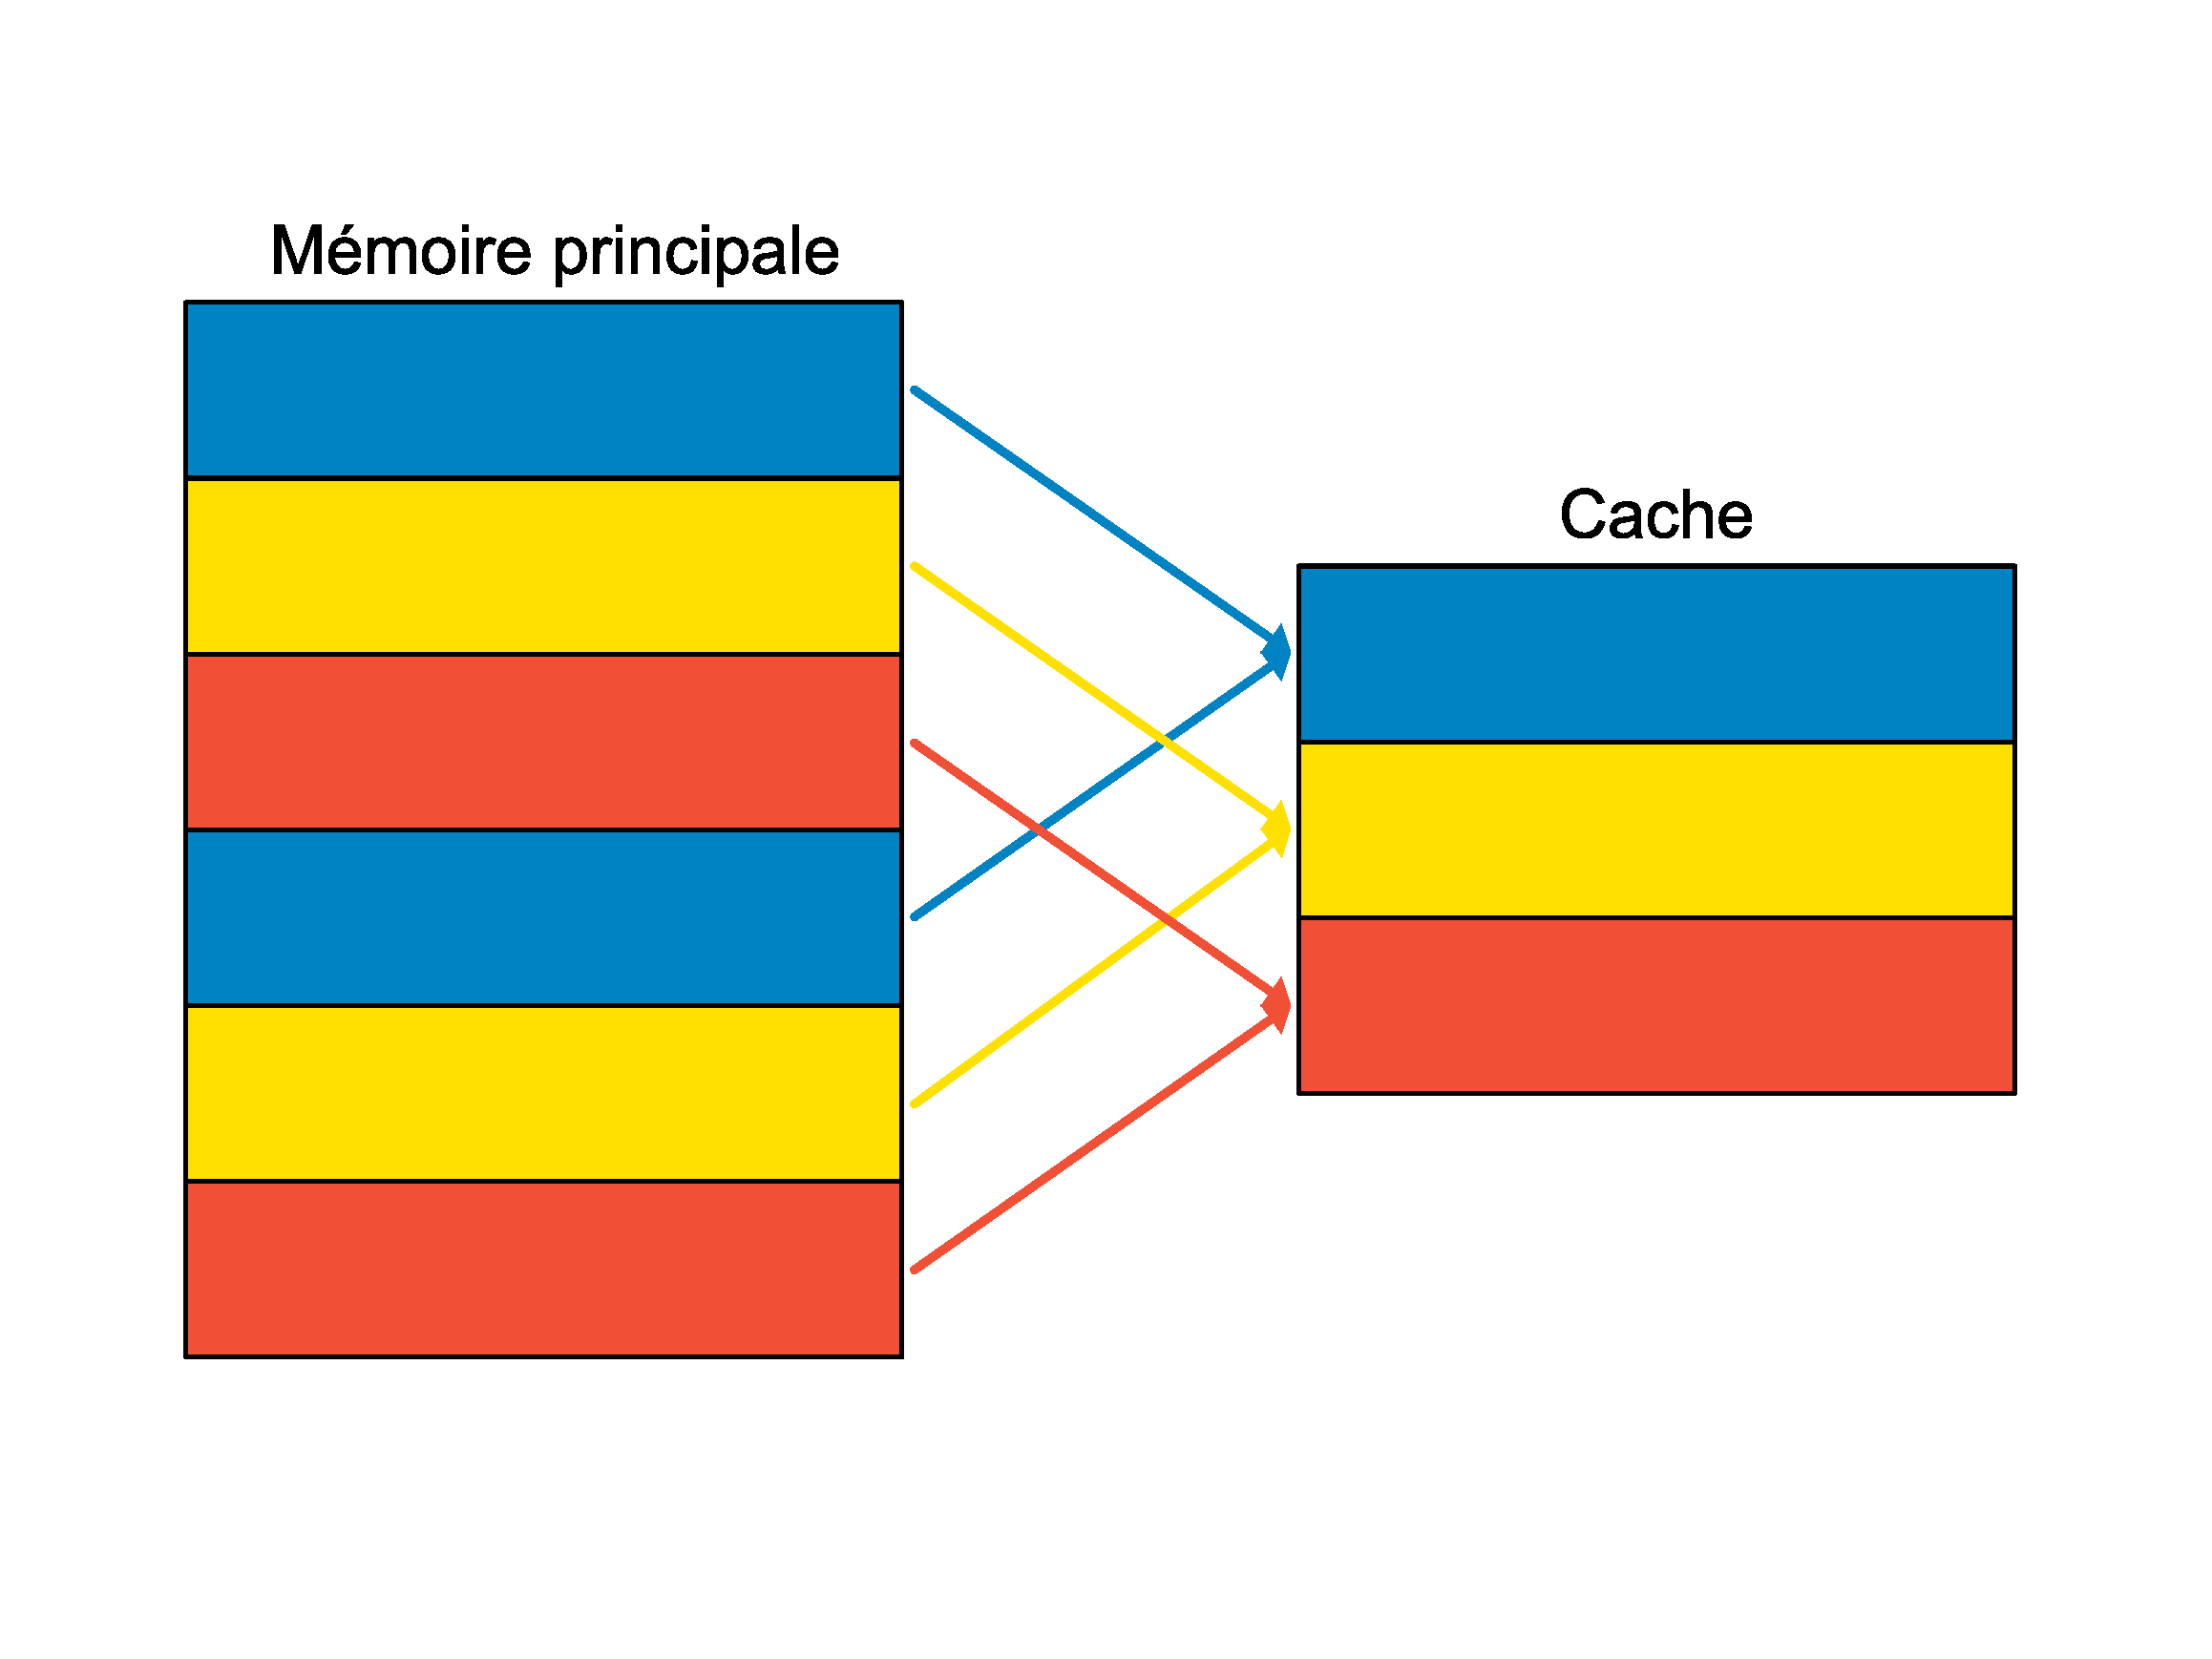
\includegraphics[width=\linewidth]{graphics/figures/cache-direct-mapping.pdf}
		\caption{\label{fig:direct_mapping}Association directe}
	\end{subfigure}
	\begin{subfigure}[t]{0.5\linewidth}
		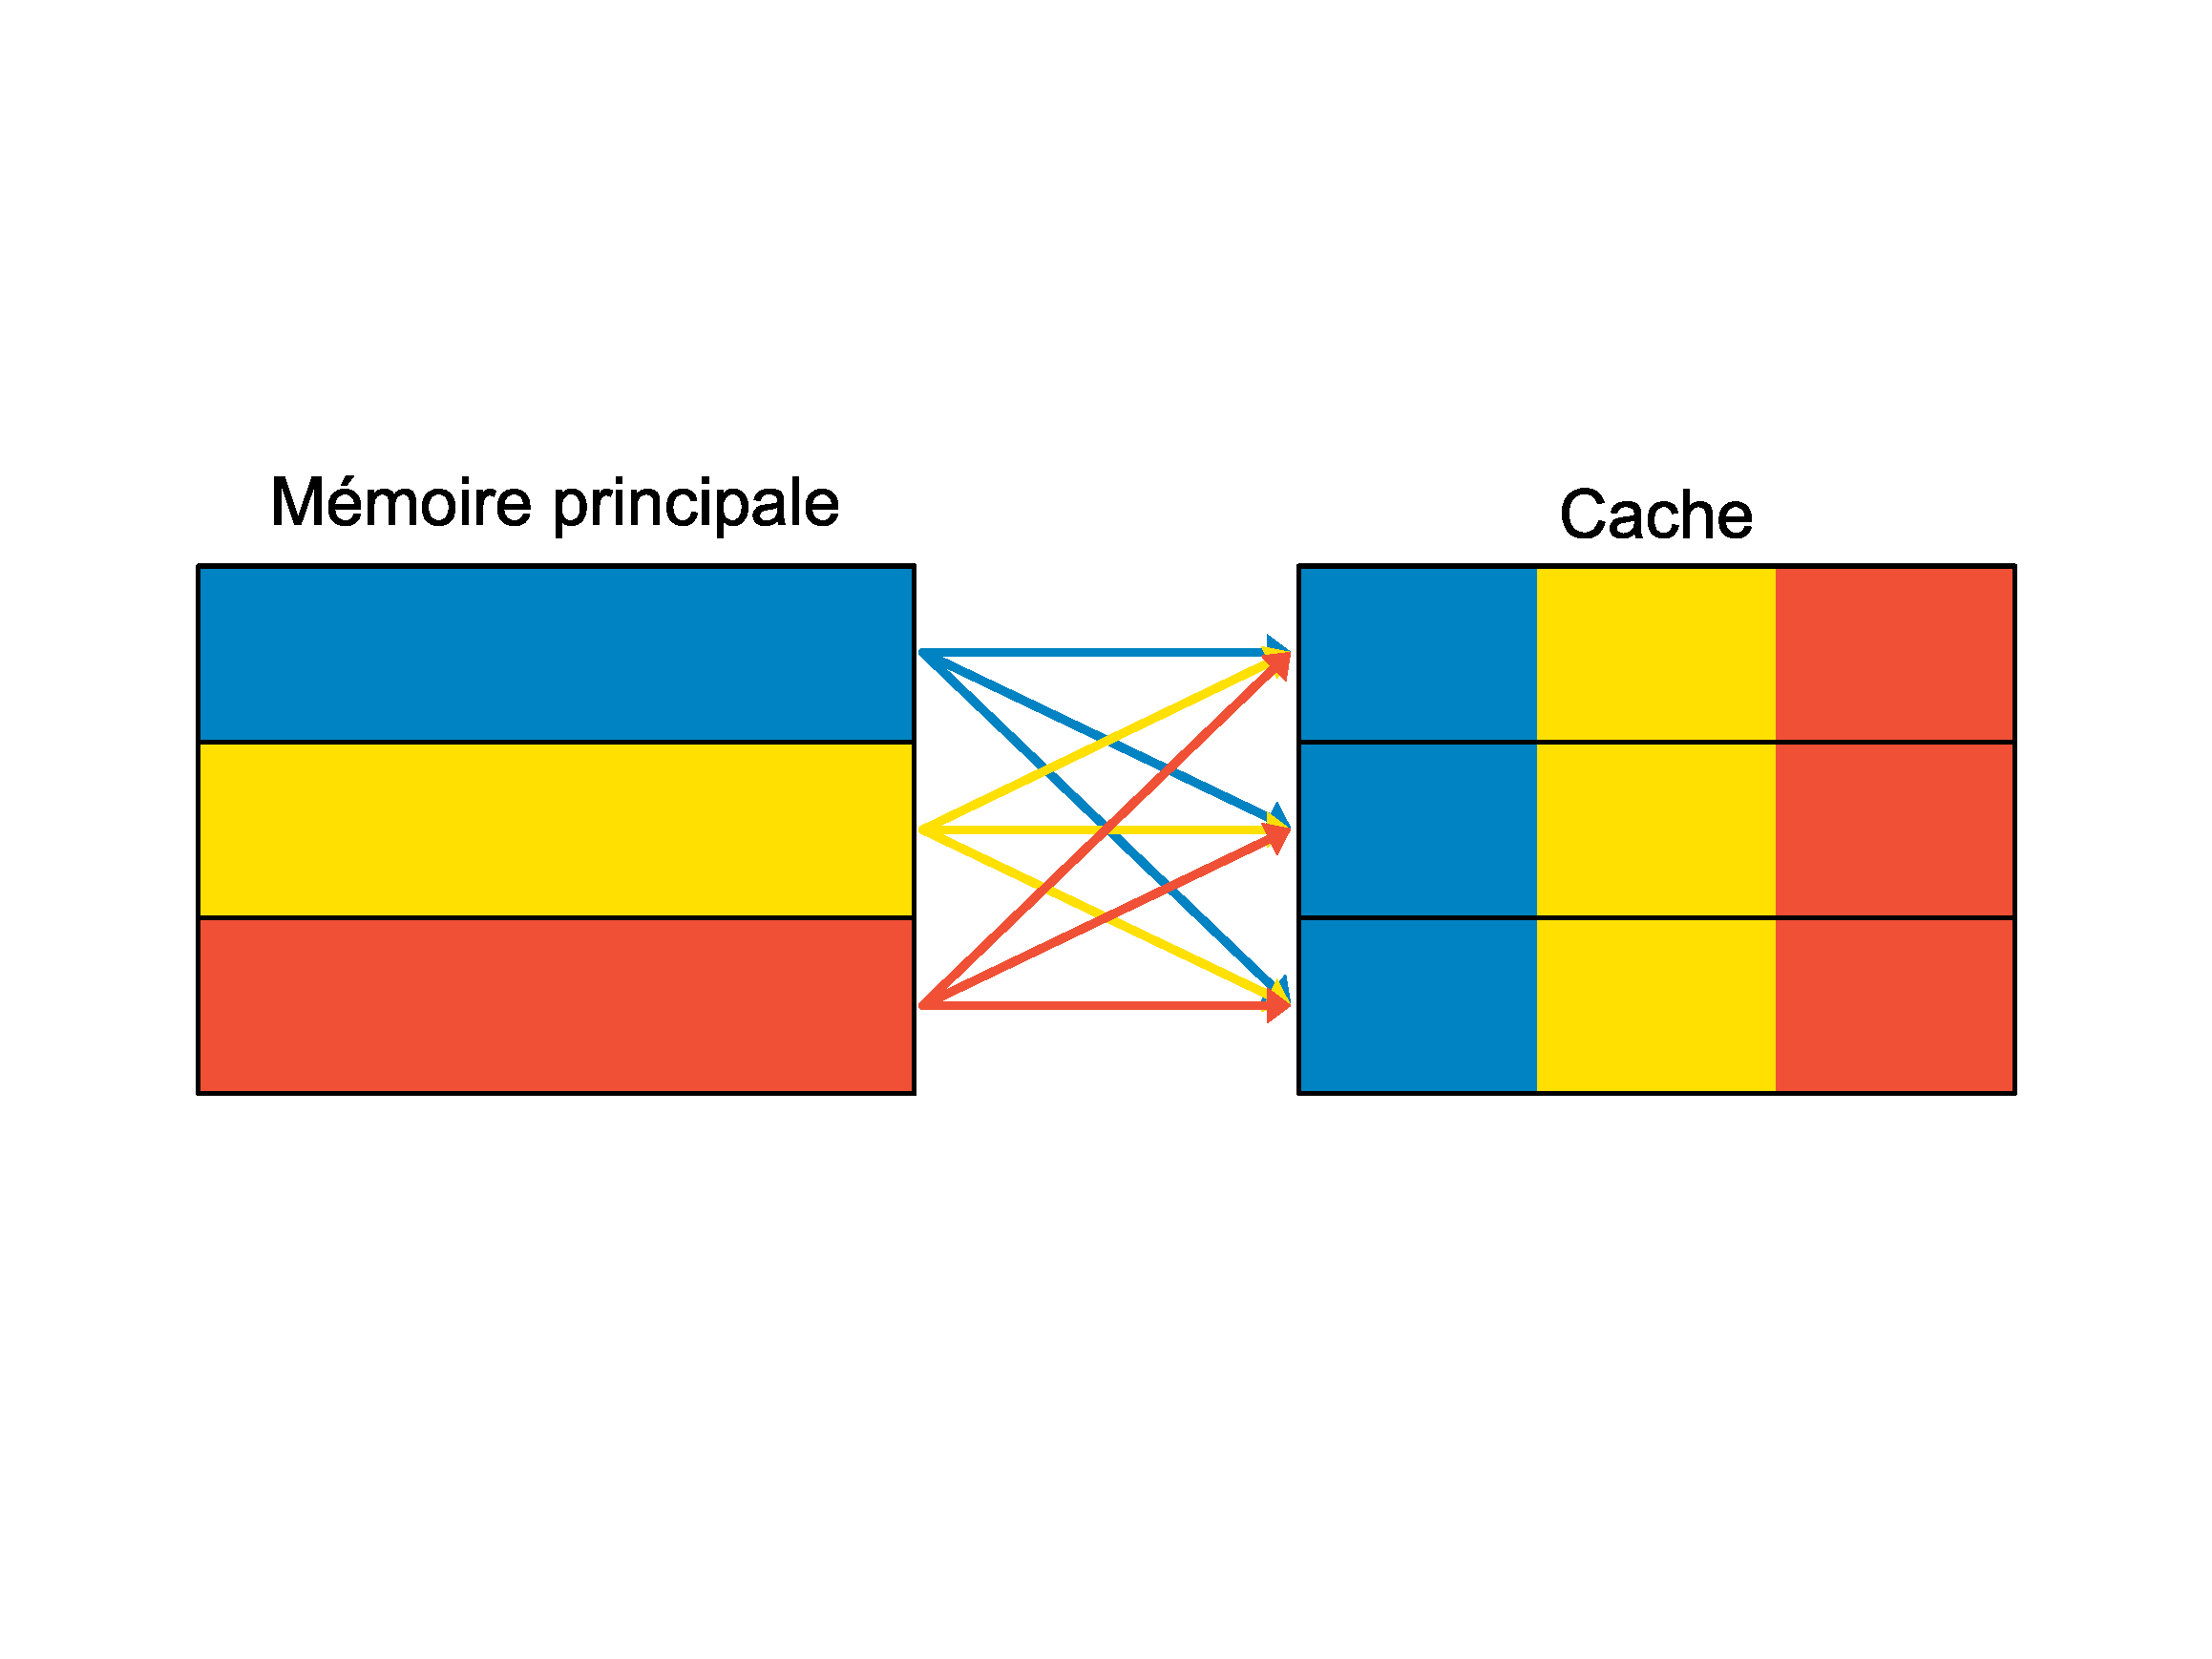
\includegraphics[width=\linewidth]{graphics/figures/cache-full-assoc.pdf}
		\caption{\label{fig:full_assoc}Associativité totale}
	\end{subfigure}
	\begin{subfigure}[b]{0.5\linewidth}
		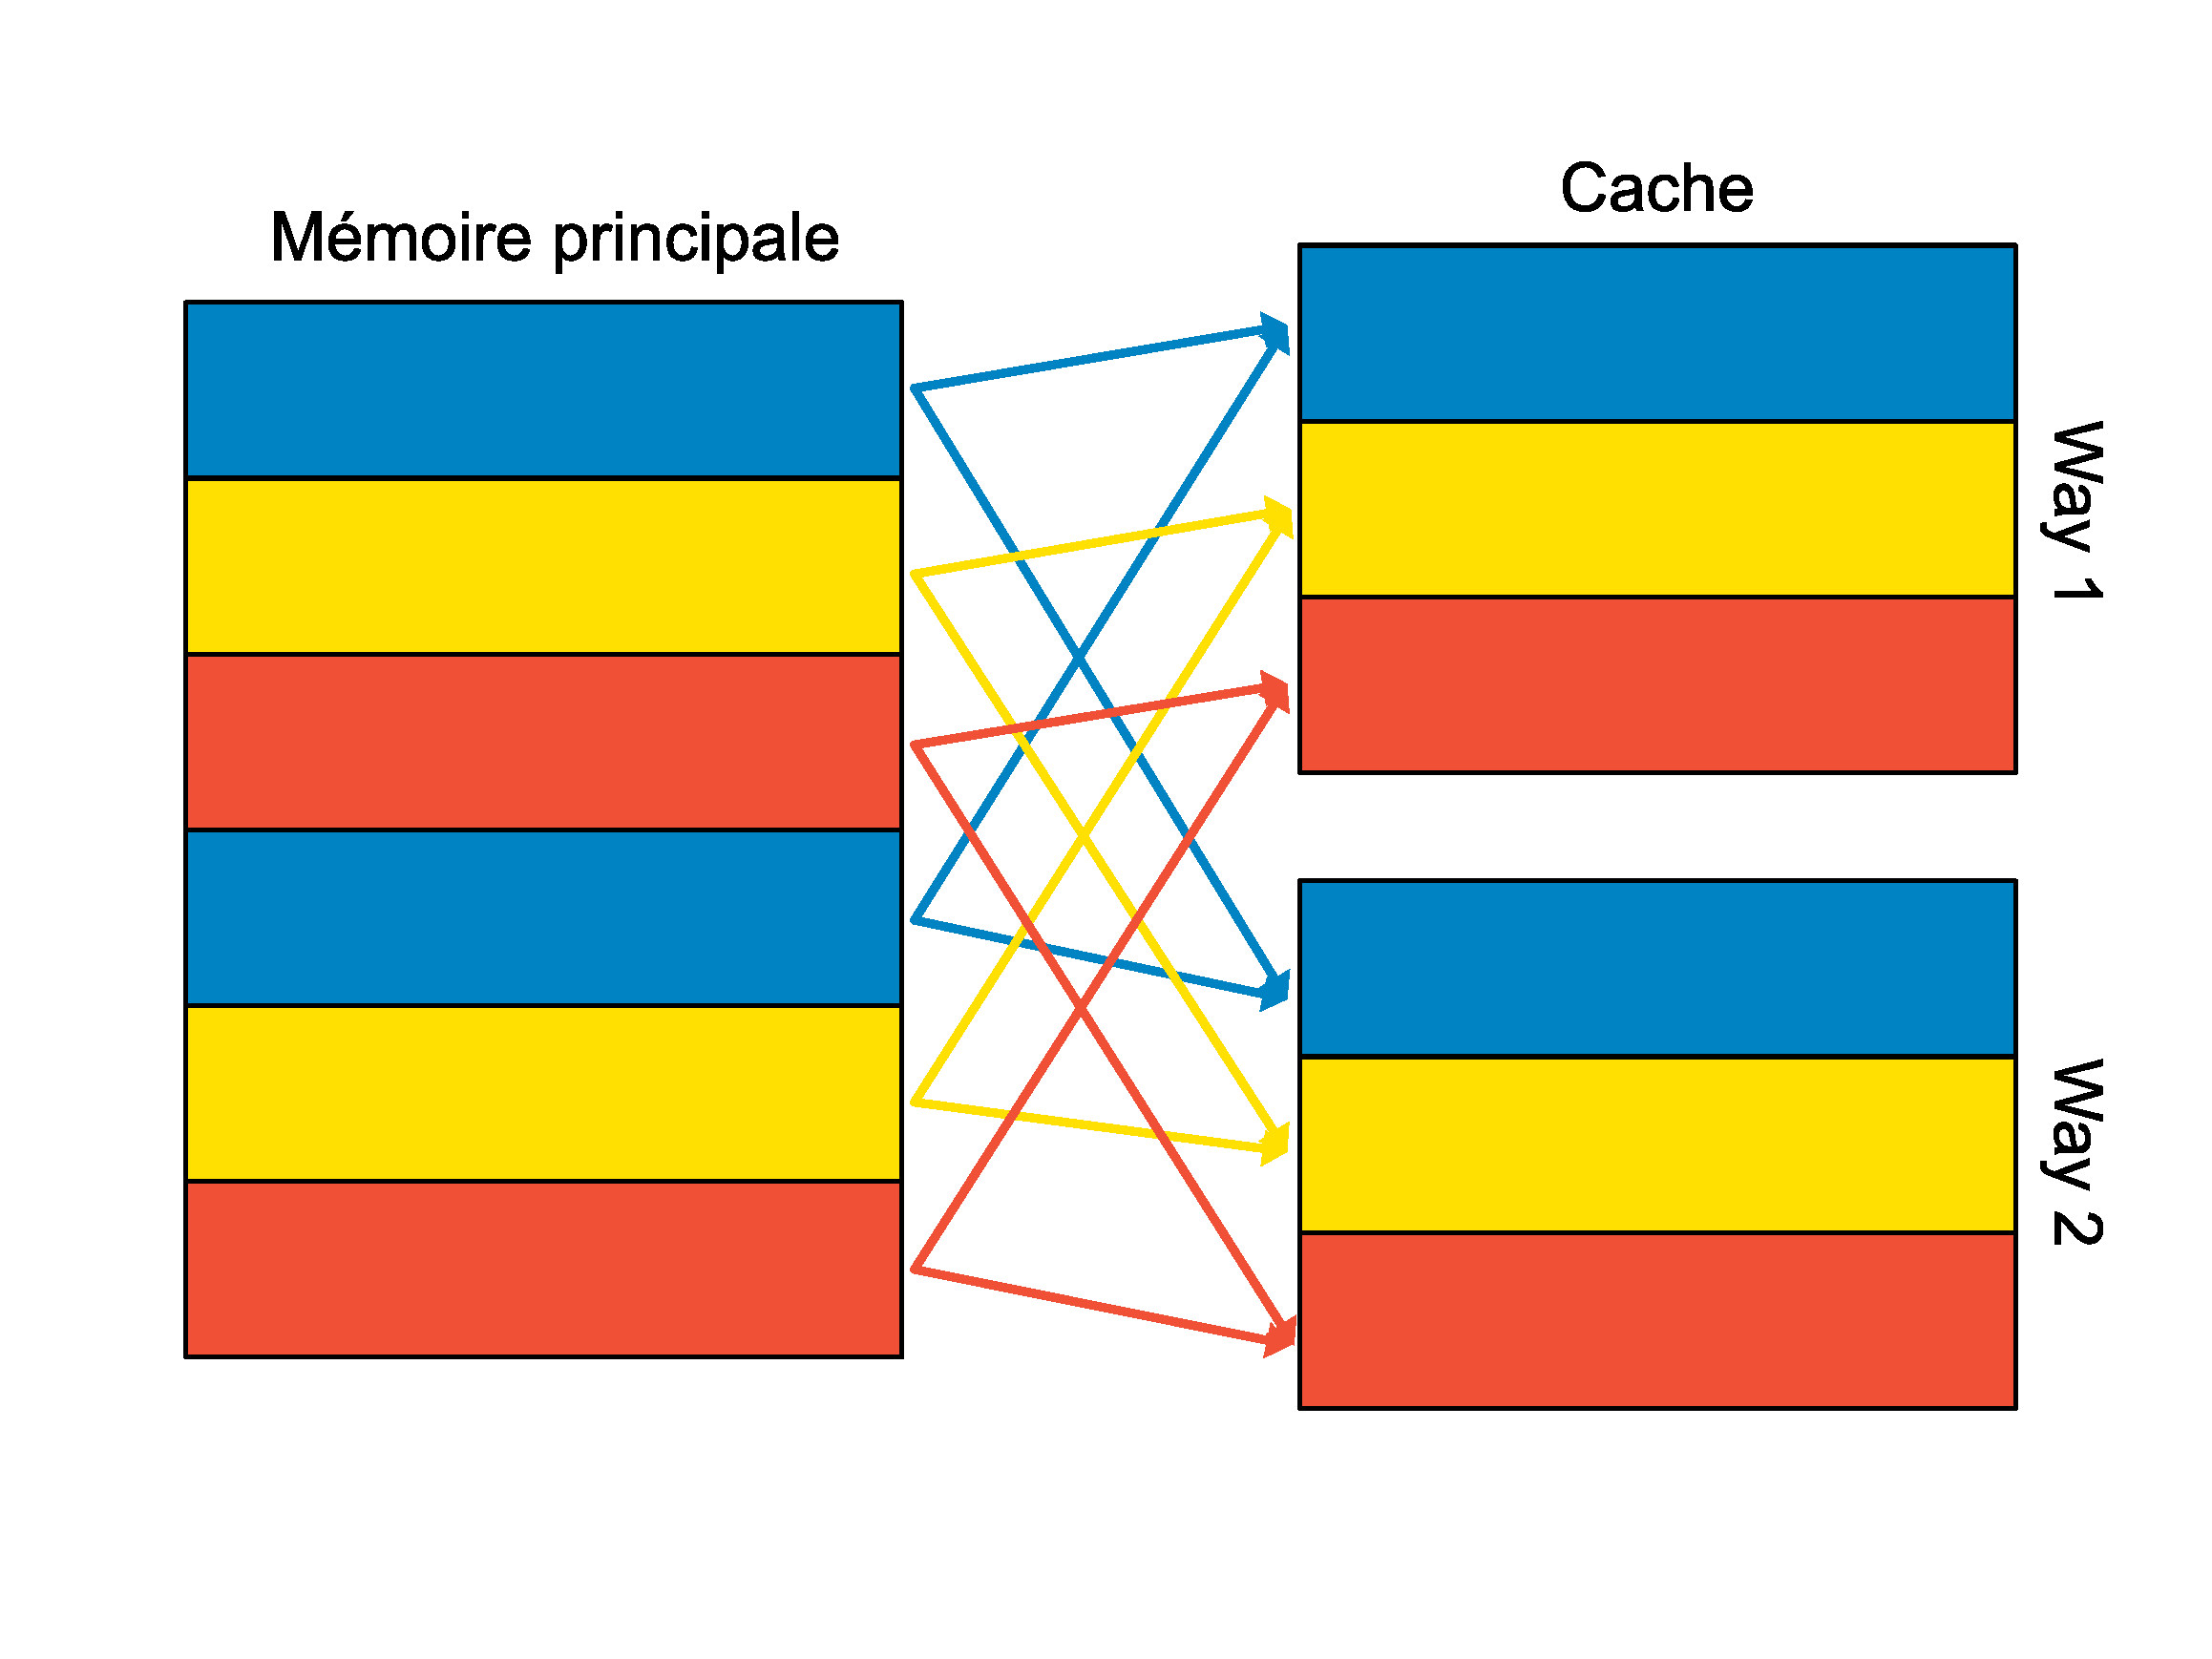
\includegraphics[width=\linewidth]{graphics/figures/cache-set-assoc.pdf}
		\caption{\label{fig:set_assoc}Associativité partielle}
	\end{subfigure}
	\caption{\label{fig:indexation_associativité} Politiques de correspondances}
\end{figure}

\subsubsection{Politiques d'écritures}

La politique d'écriture d'un cache détermine quand les données sont écrites vers le niveau supérieur.
On en dénombre deux:

\begin{itemize}
	\item \emph{Écriture directe (Write Through)} Les écritures sont immédiatement propagées vers le niveau supérieur.
	Cette politique a l'avantage de simplifier la maintenance de la cohérence entre les différents niveaux de la hiérarchie mémoire; au prix, néanmoins d'une plus grande consommation de bande passante.
	
	\item \emph{Écritures différées (Write Back)} Les données ne sont écrites vers le niveau supérieur que lors de leur remplacement.
	Les métadonnées des lignes des caches utilisant cette politique comprennent un bit \emph{dirty}, qui est activé lorsque les données de la ligne sont modifiées.
	Lors du remplacement d'une ligne, le bit dirty est d'abord testé.
	La donnée n'est alors écrite en mémoire que dans le cas où ce dernier a été activé.
	Cette politique permet de réduire le trafic vers les niveaux supérieurs de la hiérarchie mémoire, mais elle complexifie également la gestion de la cohérence des données.
\end{itemize}

\subsubsection{Politiques d'allocation}

La politique d'allocation détermine si une donnée chargée depuis le niveau de cache supérieur doit être copiée dans le cache (\emph{line fill}) ou non.
Il y a deux politiques d'allocations:

\begin{itemize}
	\item \emph{Read-allocate} Un line fill n'est effectué que lors des défauts de cache en lecture.
	Lors d'un défaut de cache en écriture, le cache n'est pas modifié et l'écriture transmise au niveau supérieur.
	\item \emph{La politique write-allocate} Un line fill a lieu lors des défauts de caches en lecture et en écriture.
	Cette politique est généralement utilisée dans les caches \emph{write-back}.
\end{itemize}

\subsubsection{Caches et interférences}

Les caches partagés sont des canaux d'interférences importants dans les processeurs modernes.
Elles peuvent être aussi bien spatiales que temporelles.
Elles entrainent trois effets indésirables majeurs:

\begin{itemize}
	\item \emph{Interférence temporelle lors de l'accès au cache} Les caches ont la capacité de traiter plusieurs accès en parallèle.
	Cette capacité peut néanmoins être excédée lors de l'utilisation en simultané du cache par plusieurs cœurs.
	Dans ce cas, des requêtes ayant dû être traitées en parallèle le sont séquentiellement induisant une latence supplémentaire.
	
	\item \emph{Contention inter-cœurs sur les lignes de cache} Les lignes de caches d'une application s'exécutant sur un cœur peuvent être remplacée au profit des lignes d'une application sur un autre cœur, ce qui a pour conséquence une augmentation des défauts conflictuels.
	Ces interférences spatiales, dites inter-cœur, ont un impact considérable sur les pires temps d'exécution, se traduisant par un surdimensionnent inacceptable du matériel.

	\item \emph{Interférence spatiale causée par les protocoles de cohérences} Lorsque des données sont partagées entre les cœurs, il faut maintenir la cohérence entre les différents caches du système.
	Les protocoles utilisés pour maintenir cette cohérence peuvent \emph{invalider} des données, provoquant ainsi une augmentation des défauts de cohérences.
	Ce problème touche surtout les systèmes adoptant le modèle symétrique.

\end{itemize}

\section{Conclusions du chapitre}

Dans cette section, nous avons présenté le problème des interférences dans les processeurs multi-cœurs destinés au marché de masse.
Ces interférences, dues aux accès concurrents aux ressources partagés entre les cœurs, sont la source de ralentissement pour des applications, empêchant ainsi l'isolation temporelle requise pour garantir la sûreté des systèmes intégrés temps-réel.
Ce problème concerne notamment le système mémoire, qui est à ce jour l'un des principaux acteurs de la performance des processeurs modernes.

% Conclusions: système embarqués => arhitecture intégrées => besoin de garantir le déterminisme => isolation temporelle

% 			pb interférence du aux partages de ressources matérielle.
% 			Principal canaux d'interférence situés dans le chemin d'accès à la mémoire
% 			Cache et DRAM concerné. Aussi bien vol de ressources qu'arbitrage.

% Transition : Interférences temporelle => pb en temps-réel. Plus de détail sur ces systèmes + approches proposée pour gérer ce problème.

Les interférences sont un problème, car elles peuvent causer la défaillance des applications temps-réel du système.
Dans le chapitre suivant, nous allons nous pencher plus en détail sur les aspects temps-réel et l'impact des interférences sur ces derniers.
Nous y présenterons également les approches proposées par la communauté scientifique pour apporter une solution au problème des interférences.\cleardoublepage
% !TEX root = ../main.tex

\chapter{Temps-réel et interférences}

Dans le chapitre précédent, nous avons vu que les processeurs multi-cœurs COTS présentent le problème des interférences dues au partage de matériel entre les cœurs.
Ces interférences étant à l'origine de ralentissements pour les applications s'exécutant en parallèle, elles posent particulièrement problème dans les systèmes temps-réel.
Ce chapitre expose les problématiques liées à l'utilisation de processeurs multi-cœur COTS dans ce type de système.

Ce chapitre est organisé de la façon suivante. 
Dans la première section, on expose des généralités sur les systèmes temps-réels, notamment sur les contraintes que ceux-ci doivent respecter.
Dans la deuxième section, nous présentons les différentes approches employées pour s'assurer du respect de ces contraintes.
Dans la troisième section, nous exposons les conséquences qu'ont les interférences dans la mise en œuvre de ces méthodes d'analyses.
Enfin, dans la quatrième et dernière section de ce chapitre, nous faisons un état de l'art des approches proposées pour la gestion du problème des interférences dans les systèmes temps-réels.

%\section{Systèmes embarqués temps-réel}

% Un système temps-réel se compose d'une ou plusieurs fonctionnalités (ou sous-systèmes) devant répondre dans un temps borné à des stimuli extérieurs.
% Le principal enjeu dans la conception d'un tel système est de s'assurer que son temps de réponse est prédictible.
% Des méthodes d'analyses ont été développées de garantir la réactivité de ces systèmes.
% Le problème qui se pose aujourd'hui est que ces méthodes sont difficiles à mettre en œuvre sur des systèmes hébergés avec du matériel moderne, à plus forte raison s'il est affecté par les interférences.

% Ce chapitre présente les systèmes temps-réel, les techniques utilisées pour guarantir la réactivité de ces systèmes, l'impact qu'ont les interférences sur leur mise en oeuvre et différentes approches proposées par la communauté pour tenter de relever les nouveaux défils posés par les interférences.


%Dans cette section, nous détaillons les systèmes temps-réels et l'implication des interférences mémoires sur ces derniers.
%Nous présenterons d'abord les deux types d'architectures embarqués et les contraintes qu'elles apportent.
%Nous présenterons ensuite les contraintes temps-réels, et le processus utilisé jusqu'à présent pour garantir le respect de ces contraintes.
%Finalement, nous nous pencherons plus en détail sur l'analyse de pire temps d'exécution.

% \section{Généralités sur les systèmes embarqués temps-réel}

% \subsection{Architecture des systèmes embarqués}

% Un système embarqué assure un certain nombre de \emph{fonctionalité} s'exécutant sur des \emph{calculateurs} reliés entre eux par le biais d'un réseau.
% Une propriété importante à maintenir est la \emph{composabilité} des fonctionnalités.
% Un système est composable si le comportement temporel et fonctionel d'une fonctionalité n'est pas affecté par celui des autres fonctionnalités du système.
% Dans ce document, sauf mention contraire, nous nous focaliserons sur le comportement temporelle des fonctionalités et parlerons donc de \emph{composabilité temporelle}.

% L'architecture d'un système embarqué définit le placement des fonctionnalités sur les différents calculateurs.
% Il y en a deux:
% \begin{itemize}
% 	\item \emph{Systèmes fédérés} Chaque fonctionnalité occupe un calculateur dédié.
% 	Cette architecture est idéale pour la composabilité, vu que les fonctionnalités sont isolées physiquement.
% 	Elle est par contre coûteuse à mettre en œuvre, la rendant difficilement applicable pour des systèmes offrant un grand nombre de fonctionnalités.

% 	\item \emph{Systèmes intégrés} Plusieurs fonctionnalités peuvent occuper un même calculateur.
% 	Cette architecture a l'avantage de réduire le coût d'implantation du système en mutualisant les calculateurs.
% 	Elle pose néanmoins le problème de garantir la composabilité du système.
% \end{itemize}

% \begin{figure}[!h]
% 	\centering
% 	\begin{subfigure}{0,4\linewidth}
% 		\centering
% 		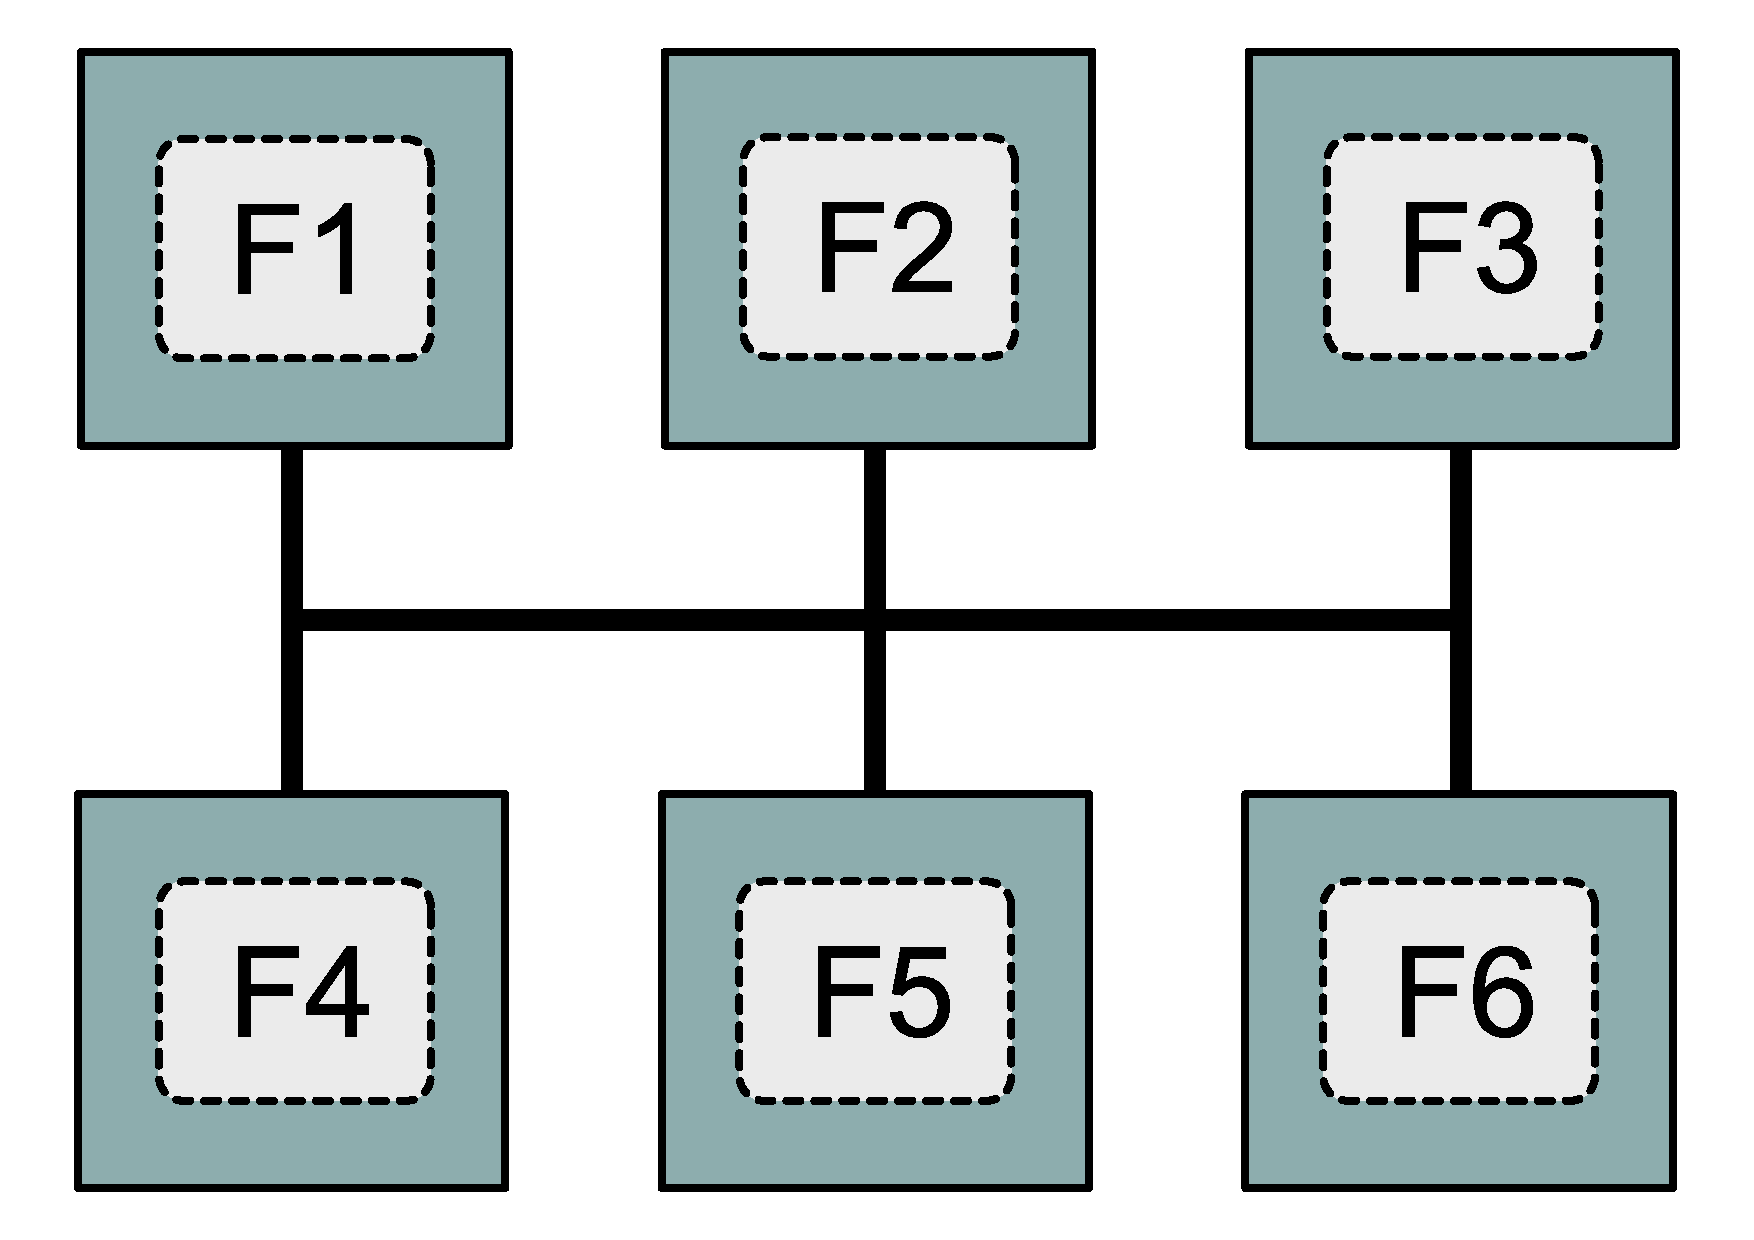
\includegraphics[width=\linewidth]{graphics/figures/federated.pdf}
% 		\caption{\label{fig:federe}Système fédéré}
% 	\end{subfigure}
% 	\begin{subfigure}{0,4\linewidth}
% 		\centering
% 		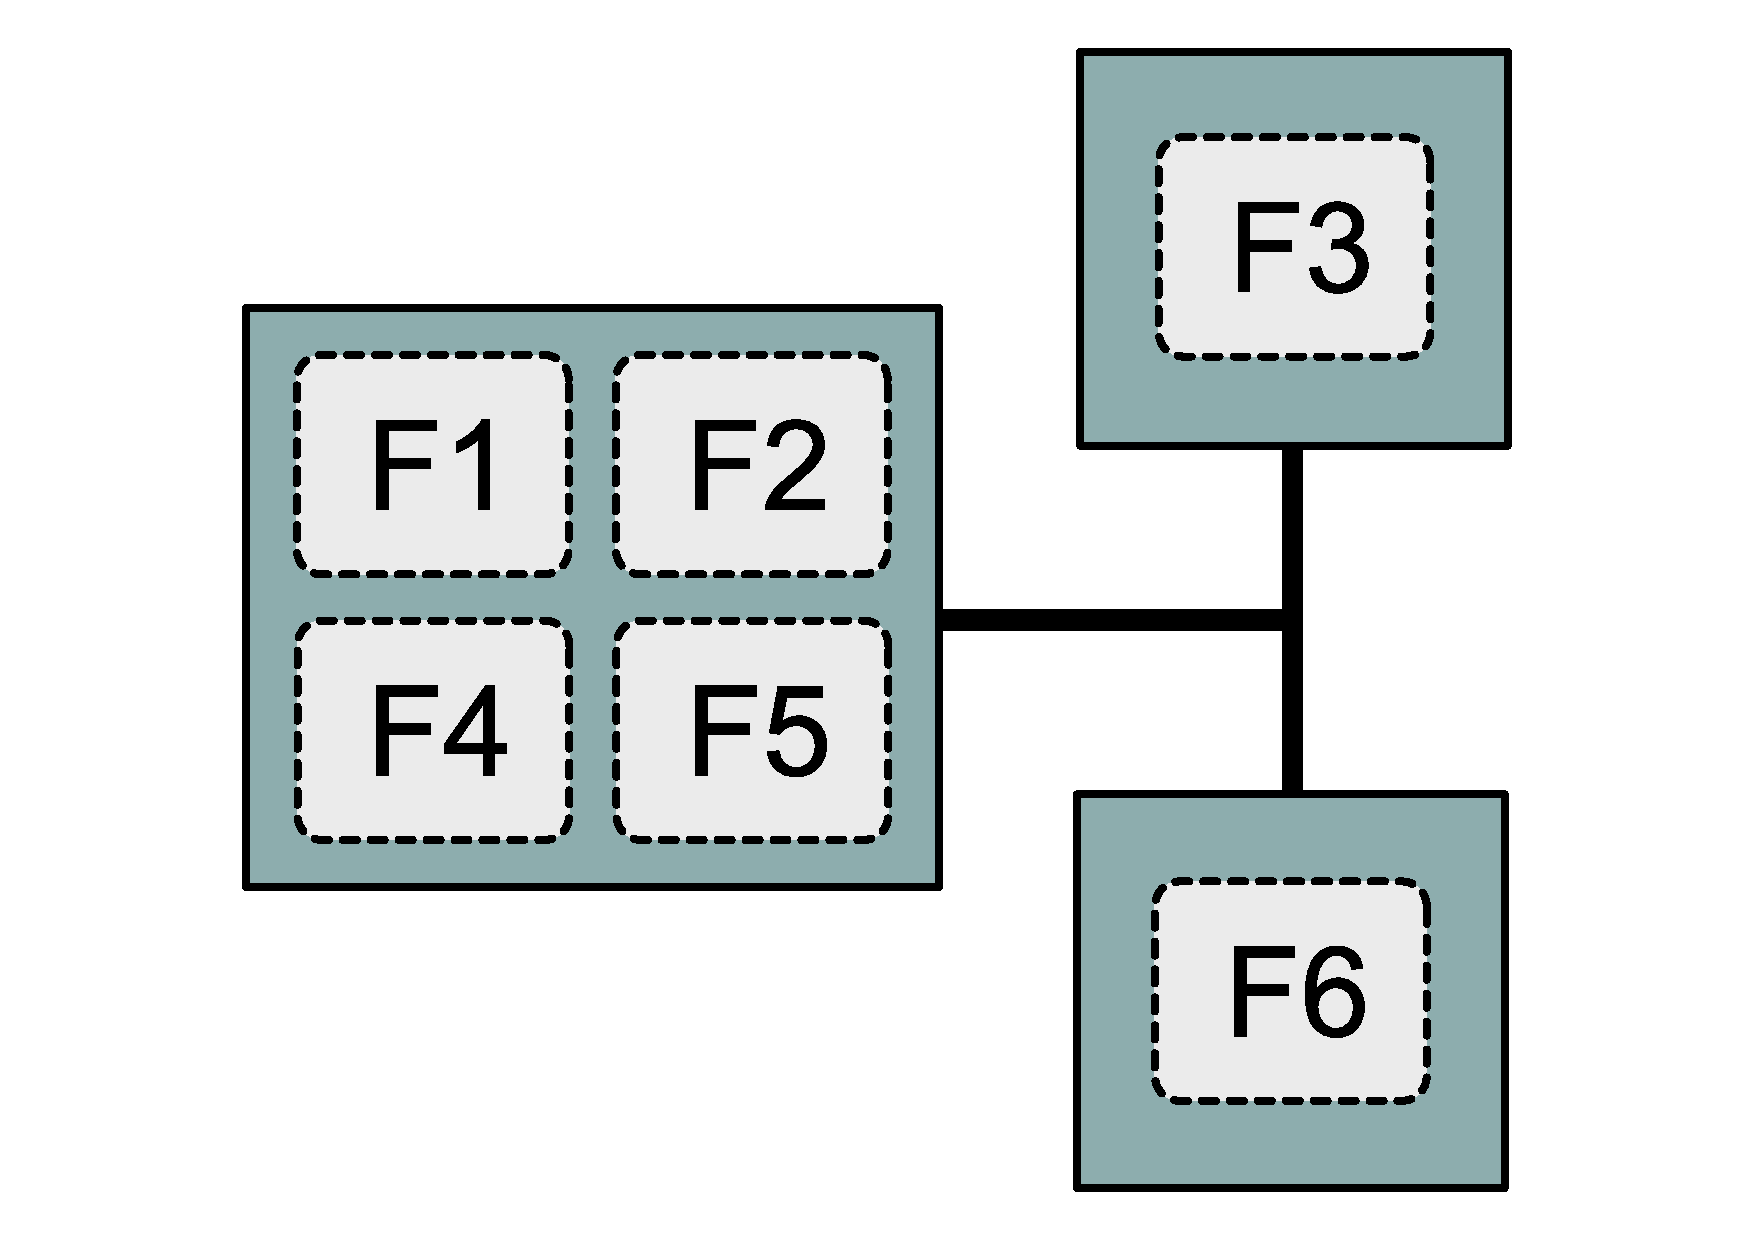
\includegraphics[width=\linewidth]{graphics/figures/integrated.pdf}
% 		\caption{\label{fig:integre}Système intégré}
% 	\end{subfigure}
% 	\caption{\label{fig:integre_federe}Architectures de systèmes embarqués}
% \end{figure}

% En théorie, l'utilisation de processeur multi-coeur offre la possibilité de pousser plus loin l'intégration des systèmes, en permettant l'exécution en parallèle de plusieurs fonctionalité sur le même calculateur.
% En pratique, malheuresement, la présence d'interférence dans les cartes multi-coeurs ne permet pas de garantir la composabilité temporelle.
% Le comportement temporel d'une fonctionalité étant alors directement affecté par les fonctionalité s'exécutant en parallèle.
% Ce problème ne permet pas d'utiliser tel quel les architectures intégrées utilisées en mono-coeur, tel qu'AUTOSAR pour l'automobile ou IMA pour l'avionique.

% Dans la section suivante, nous allons nous pencher sur l'aspect \emph{temps-réel} souvent associé aux systèmes embarqués.

% % Nous considérerons le cas, où on utilise du matériel multi-cœur pour implanter des \emph{systèmes intégrés asymétriques}.
% % À un moment donné, une fonctionnalité ne peut donc occuper qu'un seul cœur, et le but est d'exécuter plusieurs fonctionnalités en parallèle.
% % Le problème que pose la présence d'interférences est que la composabilité temporelle du système n'est plus assurée.
% % Cela a des implications pour garantir les propriétés temps-réels, nous allons maintenant voir lesquels.

\section{Généralités sur les systèmes temps-réels}

Un \emph{système temps-réel} est un système comprenant des tâches devant respecter des \emph{échéances}.
Cela ne signifie pas que le temps de réaction doit être rapide, mais qu'il doit être \emph{borné}.
Le modèle couramment utilisé, introduit par Liu et Layland~\cite{liu1973scheduling}, définit un système temps-réel comme un ensemble de \emph{tâches périodiques}.
Une tâche y est caractérisée par une période, une échéance, et une capacité qui est le temps nécessaire à l'exécution de la tâche.
Chaque tâche est activée au début de sa période et doit se terminer avant son échéance.
Si l'échéance est dépassée, cela se traduit soit par une invalidation du résultat de la tâche (on parle alors de \emph{temps-réel dur}), soit par une dégradation de la qualité de service du système (on parle de \emph{temps-réel mou}).

Un des enjeux majeurs de la conception d'un système temps-réel est d'en garantir la \emph{sûreté temporelle}, c'est-à-dire s'assurer que toutes les tâches du système respectent leurs échéances.
Le procédé usuel consiste en deux analyses successives.

\begin{enumerate}
	\item \emph{L'analyse de pire temps d'exécution} dont le but est de dimensionner les capacités des tâches du système avec le plus long temps d'exécution possible.
	\item \emph{L'analyse d'ordonnancement} dont le but est de déterminer le temps de réponse des tâches du système pour une politique d'ordonnancement donnée.
\end{enumerate}

Un système est dit \emph{ordonancable} si on peut montrer  que le temps de réponse de toutes les tâches du système est inférieur ou égal à son échéance.
Un exemple de système ordonancable et son ordonnancement est donné figure~\ref{fig:exemple_ordonancement_tr}.

\begin{figure}
	\begin{subfigure}{0,6\linewidth}
		\centering
		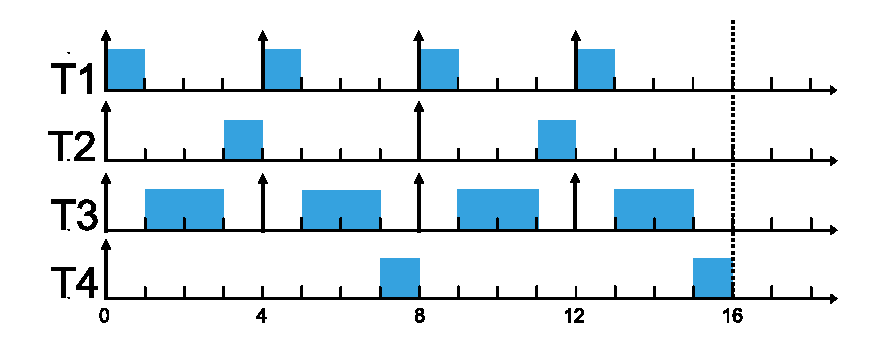
\includegraphics[width=\linewidth]{graphics/figures/sched_rt.pdf}
	\end{subfigure}
	\begin{subfigure}{0,4\linewidth}
		\centering
		\resizebox{0.9\linewidth}{!}{
			\begin{tabular}{r c c c c}
			\toprule
			& T1 & T2 & T3 & T4 \\
			\midrule
			Période  & 4 & 8 & 4 & 16 \\
			Capacité & 1 & 1 & 2 & 2  \\
			Échéance & 4 & 8 & 4 & 16 \\
			\bottomrule
			\end{tabular}
		}
	\end{subfigure}
	\caption{\label{fig:exemple_ordonancement_tr}Exemple d'ordonnancement obtenu avec la politique \emph{Earliest Deadline First}.}
\end{figure}

Ce processus repose sur une hypothèse forte, qui est que le pire temps d'exécution d'une tâche est indépendant des autres tâches du système.
En d'autres termes, il repose sur la composabilité du système. Or, nous avons vu que cette dernière n'est pas assurée en présence d'interférences.
Le choix du matériel a donc un impact important sur l'analyse de pire temps d'exécution.
C'est ce problème que nous allons étudier dans le reste de ce chapitre.

\section{Analyse de pire temps d'exécution en mono-cœur}

Dans un système temps-réel, on suppose que la capacité des tâches correspond au temps nécessaire au parcours de leur plus long chemin d'exécution\footnote{La longueur est ici exprimée en temps} sur une plateforme matérielle donnée.
Ce temps est désigné par le terme \emph{WCET}\footnote{Worst Case Execution Time}(figure~\ref{fig:terminologie_wcet}).
Le but de l'analyse de pire temps d'exécution est de borner le WCET.
Cette analyse se doit d'être \emph{sûre} et \emph{précise} : le WCET estimé ne doit pas être inférieur au WCET réel (sûreté) et il doit s'en approcher autant que possible (précision).

% L'analyse de pire temps d'exécution a pour but de déterminer le pire temps d'exécution (\emph{Worst Case Execution Time ou WCET}) d'une tâche sur un matériel donné.
% Comme illustré dans la figure~\ref{fig:terminologie_wcet}, cela que l'on cherche à déterminer le temps d'exécution le plus long parmi tous les temps d'exécution possibles.
% Le but de l'analyse est de calculer une borne sur le WCET qui soit à la fois sûre et précise.
% La sûreté se traduit par le fait que la borne ne doit pas être inférieure au WCET réel de la tâche, il s'agit d'un critère de correction de l'analyse.
% La précision est atteinte si la borne calculée est proche du WCET réel, il s'agit alors d'un critère de performance de l'analyse. 

\begin{figure}[!h]
	\centering
	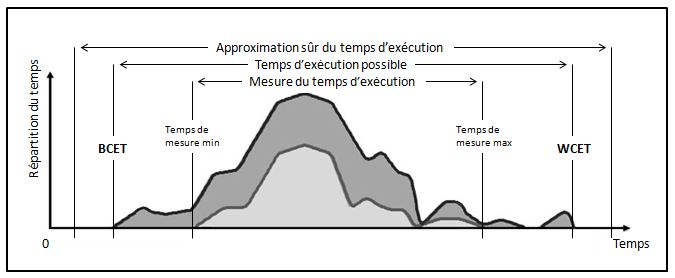
\includegraphics[width=\linewidth]{graphics/figures/termes_wcet.jpg}
	\caption{\label{fig:terminologie_wcet}
	Résumé des notions concernant l'analyse de pire temps d'exécution.
	La courbe la plus haute représente l'ensemble de toutes les exécutions possibles, tandis que la courbe la plus basse représente un sous-ensemble d'exécution mesurée.
	 (Source de l'illustration : Wikipedia)}
\end{figure}

% Il y a deux grandes familles d'approches, que nous allons maintenant détailler, pour l'analyse de pire temps d'exécution: celles basées l'analyse statique et les approches dynamiques.

Nous allons maintenant détailler deux grandes familles d'analyse du pire temps d'exécution : celles basées sur l'analyse statique de l'application (on parle de méthodes statiques) et celles basées sur des mesures (on parle de méthodes dynamiques).

\subsection{Méthodes statiques}

Les analyseurs statiques~\cite{ferdinand2004ait,lisper2014sweet,rapitime,ballabriga2010otawa,li2007chronos} de WCET le calculent sans exécuter directement les tâches. 
Une architecture générale de l'analyse employée par ces outils est décrite par Wilhelm et al.~\cite{wilhelm2009memory} et résumée par la figure~\ref{fig:process_wcet}.

\begin{figure}[!h]
	\centering
	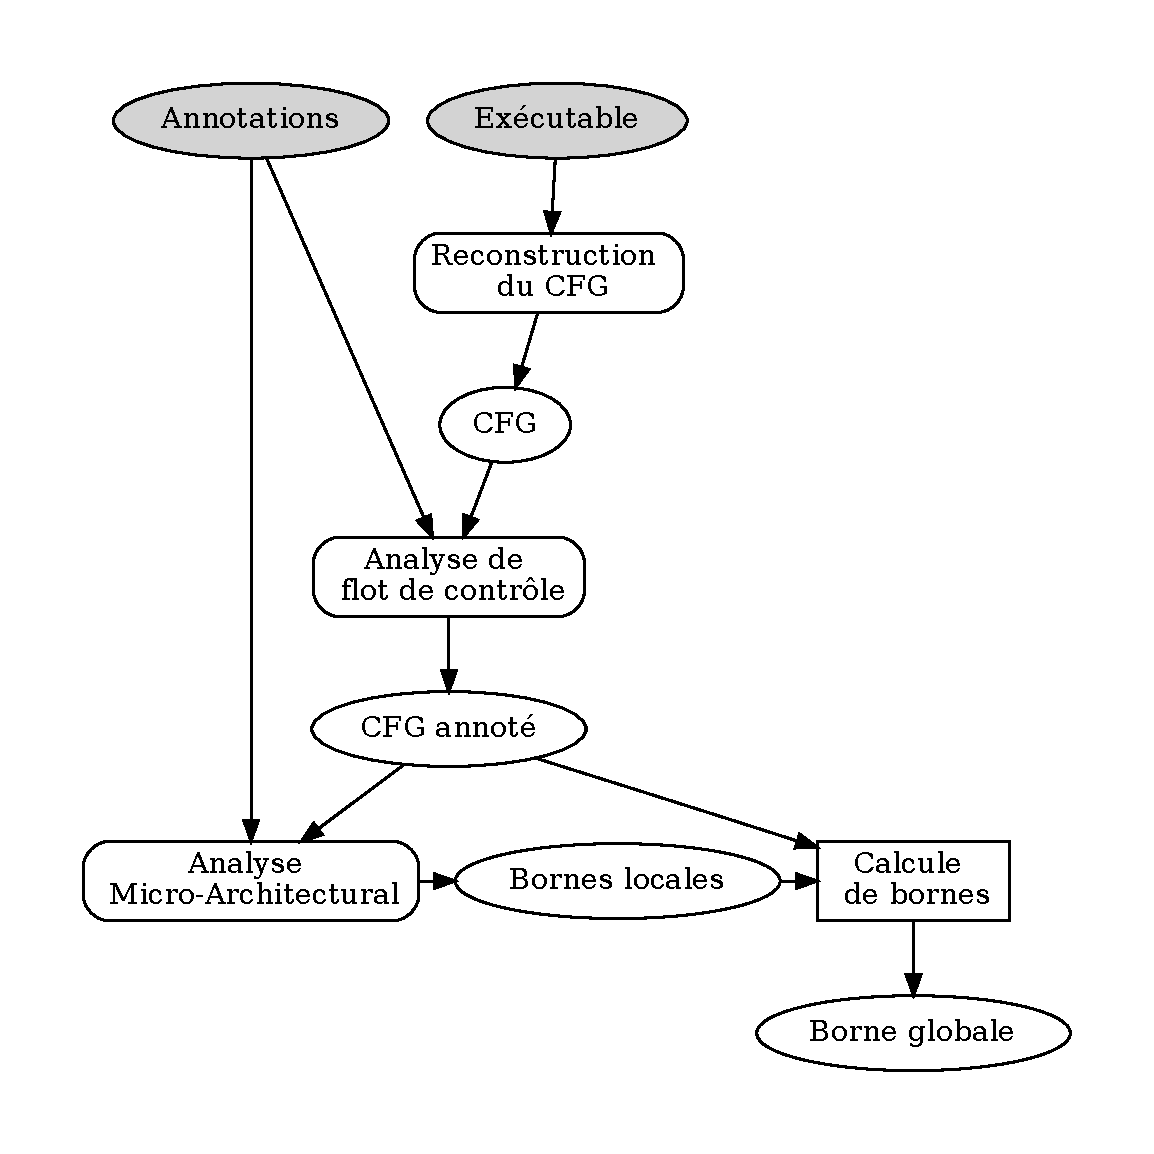
\includegraphics[width=\linewidth]{graphics/figures/wcet_static.pdf}
	\caption{\label{fig:process_wcet}Analyse statique de pire temps d'exécution}
\end{figure}

Les points d'entrée de ce type d'analyse sont le fichier binaire exécutable de la tâche analysée et un ensemble d'informations complémentaires sous forme d'annotations.
Ces informations peuvent décrire l'agencement de la mémoire, l'intervalle de valeur d'entrées de la tâche, des informations sur son flot de contrôle, etc.
Le processus de calcul de WCET à partir de ces éléments est le suivant :

\begin{enumerate}
	\item \emph{Reconstruction du graphe de flots de contrôle} Le flot de contrôle est reconstruit à partir du binaire afin d'extraire une représentation intermédiaire pour la suite de l'analyse.
	Cette étape est comparable à un frontend de compilateur.
	Le produit de cette étape est donc un \emph{graphe de flot de contrôle (CFG)}.
	
	\item \emph{Analyse du flot de contrôle} Le CFG est analysé afin de construire l'ensemble des chemins d'exécutions pouvant être possiblement être emprunté par la tâche.
	Un des objectifs de cette étape est d'éliminer de façon sûre le plus de chemins possible.
	Le produit de cette étape est un CFG annoté avec des contraintes sur le comportement dynamique de la tâche.

	\item \emph{Analyse micro architecturale} Une borne sur le temps d'exécution des blocs de bases du CFG sont calculés en utilisant un modèle abstrait du matériel.
	Le produit de cette étape est un ensemble de \emph{bornes locales}.

	\item \emph{Calcul de la borne global} Finalement, les bornes locales et les informations sur le flot de contrôle sont utilisées pour déterminer la \emph{borne globale} sur le pire temps d'exécution de la tâche.
\end{enumerate}

\subsection{Méthodes dynamiques}

L'analyse dynamique de pire temps d'exécution utilise des expériences pour déterminer le pire temps d'exécution d'une tâche.
Elle peut s'effectuer aussi bien de bout en bout que par morceau.
Dans l'analyse de bout en bout, c'est le temps complet d'une exécution de la tâche qui est mesuré.
Tandis que dans l'analyse par morceau, les mesures sont effectuées sur les blocs de bases de l'application.

Qu'elles soient de bout en bout ou par morceaux, l'analyse dynamique de pire temps d'exécution est généralement considérée comme non sûre.
D'une part, il faut s'assurer que le chemin correspondant au WCET est bien couvert par les mesures, ce qui n'est en général pas possible avec les processeurs modernes.
Ainsi, si l'on se réfère à la terminologie de la figure~\ref{fig:terminologie_wcet}, l'analyse de bout en bout ne permet techniquement d'obtenir \emph{qu'un pire temps d'exécution observé}.
Elles peuvent néanmoins être utilisées pour étudier la variabilité des temps d'exécution d'une tâche, ou encore pour valider les résultats de l'analyse statique.

\subsection{Défis de l'analyse de pire temps d'exécution}

Qu'elle soit statique ou dynamique, la complexité de mise en œuvre de l'analyse de pire temps d'exécution est fortement liée à la complexité du matériel.

Le chemin d'exécution avec le WCET dépend à la fois des données en entrée de la tâche et de l'état dans lequel se trouve le matériel.
Ces deux données étant en général difficiles à déterminer à l'avance.
Plus le matériel est complexe, plus le nombre d'états dans lequel celui peut se trouver (et donc le nombre de cas à considérer) est grand.
Cela entraine des problèmes d'explosion combinatoire concernant aussi bien les méthodes statiques (il faut considérer plus de cas dans l'analyse) que les méthodes dynamiques (la couverture de tests à fournir est plus grande).
% Cela se traduit par un problème d'explosion combinatoire dans les approches statiques, et par une couverture de tests difficile à atteindre dans les .

De plus, les processeurs modernes posent le problème du temps d'exécution des instructions.
En effet, ce dernier n'y est pas fixe.
Il dépend de l'historique des instructions exécutées précédemment.
D'une part, cela rend difficilement applicable l'analyse dynamique par morceau sur ce type de matériel.
D'autre part, cela complique l'analyse micro architecturale dans les approches statiques.
En effet, le modèle abstrait du matériel doit alors prendre en compte l'effet de composants tel que les pipelines ou les caches pour déterminer les bornes locales de la tâche.
Cela requiert un niveau d'information élevé sur le matériel qui n'est pas toujours disponible, à plus forte raison sur du matériel grand public.
De plus, le comportement dans le pire cas des composants peut conduire à des bornes très grandes.

Enfin, le dernier problème qui se pose est la présence d'anomalies temporelles sur le matériel récent.
Une anomalie temporelle survient lorsque le pire temps global n'est pas composés uniquement de pires temps locaux.
La figure~\ref{fig:anomalie} illustre un exemple d'anomalie causé par le réordonnancement des instructions au sein du pipeline d'un processeur.
On peut y voir deux ordonnancements d'instructions partiellement dépendantes entre elles.
Les séquences sont identiques à l'exception de l'instruction A qui met plus de temps à s'exécuter dans le premier cas que dans le second.
L'anomalie est que c'est ce dernier cas qui met le plus de temps à s'exécuter au final.
Si on ne peut pas borner \emph{par une constante} la différence de temps d'exécution causée par les anomalies temporelles, on parle alors d'\emph{effet domino}.
Les processeurs modernes présentent en général à la fois des anomalies temporelles et des effets dominos.
La présence d'anomalie temporelle a plusieurs conséquences:
\begin{itemize}
	\item Il n'est pas sûr d'utiliser l'approche gloutonne pour déterminer le chemin d'exécution correspondant au WCET.
	\item On ne peut pas identifier un pire état initial, permettant par exemple de procéder de façon sûre à de l'analyse dynamique par morceau.
	\item Une architecture matérielle présentant des anomalies temporelles et des effets dominos est dite \emph{non-compositionelle}~\cite{hahn2015towards}.
	Une architecture est compositionnelle si on peut décomposer le pire temps d'exécution totale en la somme des contributions au pire temps d'exécution des éléments du système.
	La conséquence est que l'on ne peut pas modulariser aisément l'analyse de ce genre de matériel.
\end{itemize}

\begin{figure}
\centering
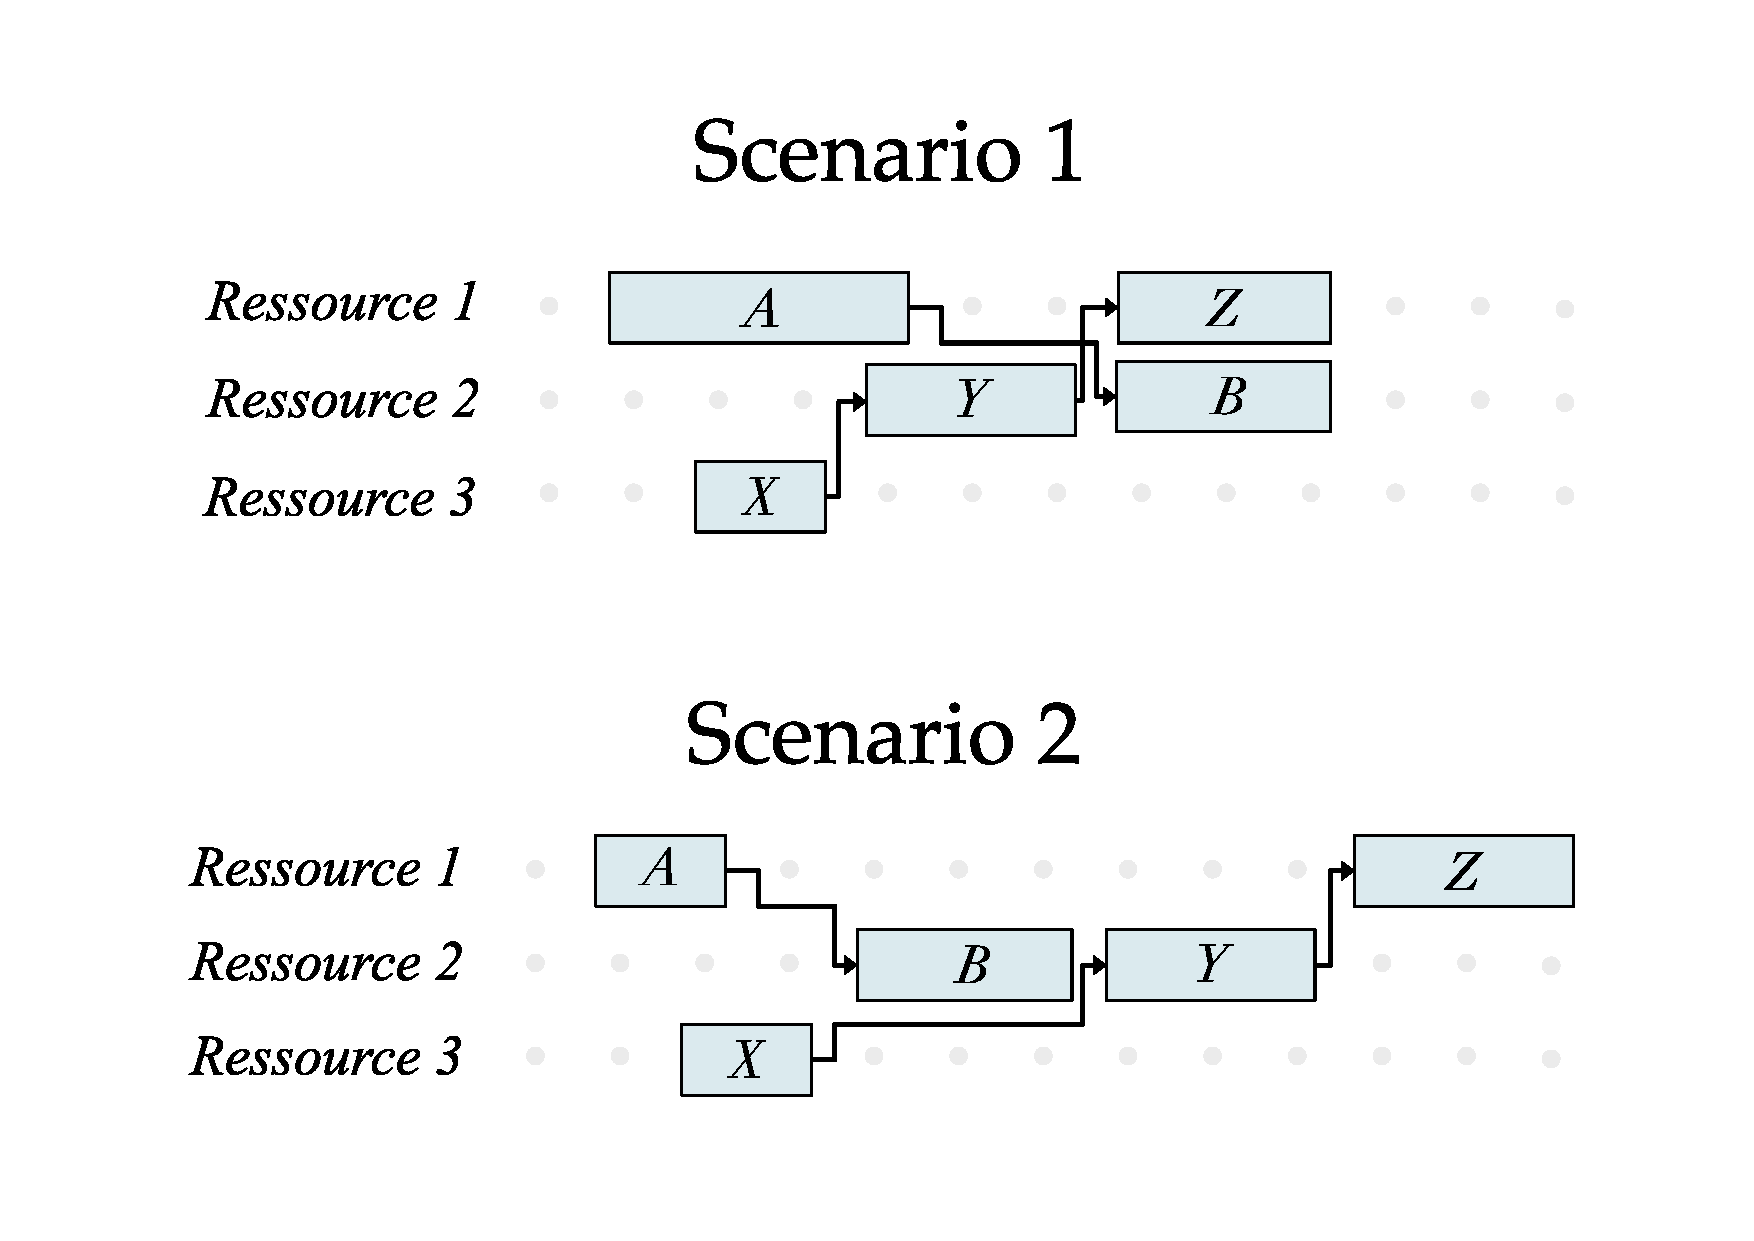
\includegraphics[width=0.7\linewidth]{graphics/figures/anomalie2.pdf}
\caption{\label{fig:anomalie} Exemple d'anomalie temporelle due à un réordonnancement d'instructions. Les flèches indiquent des dépendances entre instructions.}
\end{figure}

\section{\label{section:impact-interferences-wcet}Impact des interférences}

L'utilisation de matériel multi-cœur COTS a un impact très important dans le cadre des systèmes temps-réels.
Elle remet notamment en question l'applicabilité des méthodes existantes pour vérifier la sûreté temporelle de ces systèmes.

Les interférences peuvent causer des ralentissements plus ou moins importants aux tâches temps-réels, qui s’ ils ne sont pas pris en compte peuvent causer un sous-dimensionnement du système entrainant des dépassements d'échéances.
Le ralentissement subi par une tâche dépend à la fois de son utilisation du système mémoire, mais aussi de la pression exercée sur celui-ci par les autres tâches du système.
Dans ces conditions, il devient  difficile d'évaluer le pire temps d'exécution indépendamment du contexte d'ordonnancement, remettant ainsi en cause l'approche en deux étapes utilisées dans les systèmes mono-cœurs.
Notons également que dans des systèmes à criticité mixte, le comportement exact des tâches non critique n'est en général pas connu, empêchant ainsi l'évaluation du contexte d'ordonnancement.

La nature du matériel utilisé pose également problème.
Tout d'abord, les processeurs multi-cœurs COTS sont en général très complexes et leur comportement n'est en général pas documenté exhaustivement.
Dans ces conditions, construire un modèle abstrait d'un tel processeur est difficile et peut conduire à l'utilisation d'hypothèses simplificatrices souvent très pessimistes.
Ensuite, ces processeurs sont conçus pour offrir de bonnes performances en moyenne, et donc le comportement des mécanismes utilisés peut être très mauvais dans les pires cas.
Enfin, la non-compositionnalité des architectures employées aggrave encore ce problème, dans la mesure où elle complique la modularisation de l'analyse.

Dans les faits, les points que nous venons de soulever entrainent l'adoption d'hypothèse très pessimistes, et donc le surdimensionnement des systèmes.
D'un point de vue industriel, tout l'enjeu est de pouvoir dimensionner de façon sure, mais aussi efficace, les systèmes temps-réel en tenant compte des interférences.
Dans la section suivante, nous allons présenter l'état de l'art des interférences.

\section{Temps-réel et interférences}

% Les méthodes utilisées jusqu'alors pour s'assurer du respect des contraintes temporelles ont initialement été dévelopée pour des systèmes mono-coeurs.
% En particulier, le pire temps d'exécution des tâches est déterminé en \emph{isolation}. 
% C'est à dire que ce temps ne varie pas en fonction du contexte d'ordonancement.
% Cette hypothèse est évidement invalidée dans le cas de système multi-coeur utilisant du matériel sujet aux interférences.
% Ne pas prendre l'effet de ces interférences peut conduire à sous-estimer le pire des tâches temps-réels, et donc conduire à des dépassement d'échéances.

% Les interférences posent un sérieux problème d'allocation de ressources dans les systèmes temps-réels.
% À cet effet, elles font partie des préocupations de la communauté temps-réels depuis la fin des années 2000.
% L'enjeu est de pouvoir dimensionner les systèmes temps-réels de façon sure et efficace.
% C'est à dire que le surcoût temporel estimé ne doit pas excéder les bénéfices apportés par le matériel.
% Dans cette section, nous allons présenter l'état de l'art de la gestion des interférences pour le temps-réel.
% Nous traiterons d'abords des travaux visant à calculer le surcout induit par les interférences.
% Nous nous pencherons ensuite sur les approches visant à isoler les applications s'exécutant en parallèle.
% Finalement, nous présenterons des solutions de régulation visant à fournir un filet de sécurité.

La présence d'interférences dans le matériel moderne fait partie des préoccupations de la communauté temps-réel depuis la fin des années 2000.
Nous allons, dans cette section, présenter diverses approches proposées pour apporter des solutions à ce problème.
Nous distinguerons trois grandes familles d'approches:
\begin{itemize}
	\item Les approches traitant du \emph{dimensionnement} du système en prenant en compte l'impact des interférences. Cela passe par l'extension des méthodes classiques de vérification temporelles, mais également par des études empiriques.

	\item Les approches traitant de \emph{l'isolation} des applications ont pour but de réduire, voir supprimer, les interférences. Elles peuvent aussi permettre un dimensionnement moins pessimiste des systèmes. 

	\item Les approches traitant de \emph{la régulation} ont pour but de fournir un filet de sécurité à l'exécution. Ces approches reposent sur un monitorage de l'état du système afin de détecter des situations pouvant causer des défaillances, et le cas échéant prendre des mesures appropriées.
\end{itemize}

\subsection{Calcul de pire temps d'exécution}

Un grand nombre de travaux visent à incorporer l'impact des interférences dans les analyses temporelles classiques.
L'enjeu de ces travaux est d'offrir des analyses à la fois sûres et efficaces : sûre, car l'impact des interférences ne doit pas y être sous-estimé, efficace, car il doit être aussi proche que possible de la réalité.
% c'est à dire que l'impact ne doit pas être sous estimé mais également aussi proche que possible de la réalité.
Il s'agit d'un problème difficile pour les raisons invoquées dans la section~\ref{section:impact-interferences-wcet}.
Le problème est d'ailleurs encore ouvert.
Pour un inventaire récent et détaillé des recherches dans ce domaine, nous orientons le lecteur vers l'étude de Maiza et al.~\cite{maiza2018survey} en complément de ce chapitre.

Les travaux étendant la vérification des propriétés temporelles des systèmes temps-réels se distinguent à la fois par le choix de l'analyse étendue (de pire temps d'exécution ou d'ordonnancement) et la modélisation des interférences.

% La transpositions des méthodes de vérifications temporelles utilisées dans les systèmes mono-coeurs aux systèmes multi-coeurs est un problème difficile, faisant d'ailleurs encore aujourdh'ui l'objet d'un effort important de recherche.
% Une étude détaillée sur les dernières avancées dans ce domaine a été proposée par Maiza et al.~\cite{maiza2018survey}.
% Les travaux se distinguent aussi bien par le type d'analyse étendue(de pire temps d'exécution que de l'analyse d'ordonancement) que par la modélisation des interférences.

\paragraph{Extension de l'analyse de pire temps d'exécution}
Peu de travaux incorporent les interférences dans l'analyse de pire temps d'exécution. 
Cela peut s'expliquer par l'absence de contexte d'exécution, rendant difficile la modélisation des interférences.
On peut néanmoins, prendre en compte les interférences dans cette analyse en suivant deux approches:
\begin{itemize}
	\item L'\emph{approche de Murphy}~\cite{abel2013impact}\footnote{Nommée d'après la loi éponyme.} consiste à considérer toutes les interférences possibles pour chaque accès.
	Pour pouvoir appliquer cette approche, le pire surcoût possible par accès doit être borné.
	Ce n'est pas toujours possible, et dans le cas où on pourrait le faire, les bornes calculées sont en général très pessimistes~\cite{perret2016predictable,nowotsch2014multi}.

	\item Les \emph{approches complètement intégrées} visent à analyser simultanément toutes les tâches s'exécutant en parallèle.
	Ce type d'analyse offre théoriquement une précision idéale, le surcoût temporel estimé étant déterminé à partir de tous les entrelacements d'accès possible sur les ressources partagées.
	En pratique, l'applicabilité de ce type d'approche reste incertaine.
	En cause le niveau d'information requis sur toutes les tâches du système, mais aussi la complexité du calcul.
\end{itemize}

\paragraph{Extension de l'analyse d'ordonnancement}
Les interférences peuvent également être intégrées dans le calcul du pire temps de réponse.
C'est-à-dire pendant l'analyse d'ordonnancement.
Cette approche permet de prendre en compte le contexte d'ordonnancement, en particulier la pression éventuelle sur les ressources partagées.
Néanmoins, lorsque ce contexte n'est pas disponible, par exemple dans le cas où le comportement des autres tâches n'est pas connu, des hypothèses pessimistes de consommation peuvent être employées.
Un certain nombre de travaux repose sur l'utilisation de \emph{courbes d'arrivée} comme abstraction de la consommation de ressources partagées.
Ces courbes sont des fonctions associant à chaque intervalle de temps le nombre d'occurrences d'un événement.
Elles permettent donc de borner quantitativement la consommation de ressource mémoire d'une tâche.
Des travaux récents~\cite{oehlert2018compiler} montrent que ces courbes peuvent être déterminées par des méthodes d'analyse statiques.

\paragraph{Modèles d'interférences des composants du système mémoire}
L'estimation de l'impact des interférences, quel que soit la méthode employée, repose sur un modèle plus ou moins détaillé du système mémoire.
Les composants étudiés dans la littérature sont les bus d'interconnexions, les caches, et la DRAM.

La principale difficulté concernant les bus d'interconnexion est le manque d'information sur la politique d'arbitrage utilisée en cas d'accès concurrents.
Notons que certaines politiques d'arbitrage n'ont pas de temps de réponse borné.
Les articles traitant des bus font en général des hypothèses sur cette politique, en considérant par exemple une politique TDMA.
Cela pose problème pour appliquer ces résultats lorsque l'on cible du matériel COTS.

Les caches ont également fait l'objet d'une attention particulière.
La majorité des travaux sont consacrés aux interférences spatiales, et donc à déterminer le nombre de défauts de caches supplémentaires induit par les interférences.
Ces approches ont d'abord été limitées aux caches d'instructions~\cite{2008_Yan_WCET_analysis_for_Multi_Core_processors_with_shared_L2_instruction_caches,zhang2009accurately,2009_hardy_using_bypass_to_tighten_WCET_estimates_for_Multi_Core_processors_with_shared_instruction_caches}, puis étendues aux caches de données~\cite{2010_Lesage_shared_data_caches_conflicts_reduction_for_WCET_computation_in_Multi_Core_architectures}.
Si dans les caches partagés, les interférences spatiales les plus évidentes, il ne faut pas oublier que les interférences temporelles existent.
Valsan et al.~\cite{valsan2016taming} ont montrés ce problème sur diverses architectures.
Mesurer précisément l'impact de ces interférences temporelles semble néanmoins difficile.

De multiples conceptions de contrôleur DRAM déterministe ont été proposées~\cite{2007_Akesson_Predator_A_predictable_SDRAM_memory_controller,2011_Reineke_PRET_DRAM_controller_bank_privatization_for_predictability_and_temporal_isolation,2014_Krishnapillai_ROC_A_rank_switching_open_row_DRAM_controller_for_time_predictable_systems}, mais peu d'études ont été effectuées sur les contrôleurs utilisés dans les plateformes COTS.
Wu et al.~\cite{wu2013worst} ont réalisé une des premières études de pire temps de réponse de la DRAM.
Les auteurs y font néanmoins l'hypothèse de l'absence de politique de réordonnancement, ces dernières pouvant conduire à des temps d'accès non bornés.
Cette hypothèse a ensuite été levée par Kim et al.~\cite{kim2014bounding,kim2016bounding}.
Les résultats de ces analyses restent pessimistes, et peuvent être surtout invalidés en fonction des politiques d'arbitrage effectivement implantées dans les contrôleurs.

La présence d'anomalies temporelles et d'effets dominos dans les architectures modernes pose également le problème de la compositionnalité des analyses d'interférences.
En effet, rien ne dit que la somme des retards dus aux interférences de chaque composant est supérieure ou égale au retard finalement observé.
Des approches pour prendre ce phénomène en compte ont été proposées par Hahn et al.~\cite{hahn2016enabling}, augmentant encore le pessimisme des analyses.
Réciproquement, la capacité de recouvrement des retards offerts par les processeurs modernes par le biais de mécanismes comme les pipelines et l'exécution dans le désordre ne sont pas pris en compte.

\subsubsection{Conclusions}

Les approches présentées dans cette section visent à borner de façon sûre l'effet des interférences.
Elles se heurtent néanmoins à la complexité et à l'opacité du matériel étudié.
Ainsi, des hypothèses simplificatrices sont souvent employées, remettant en cause l'applicabilité de ces travaux pour des cibles COTS.
Enfin, les bornes dérivées sont très pessimistes, au point de les rendre inutiles en pratique, le surcoût calculé compensant complètement le bénéfice apporté par le fait d'avoir plusieurs cœurs.

\subsection{Approches empiriques}

L'analyse statique du pire temps d'exécution est un problème difficile, dont la complexité de mise en œuvre croît avec celle du matériel ciblé.
Les processeurs évoluant plus vite que les approches d'analyse statiques, ces dernières sont aujourd'hui difficilement applicables au matériel moderne.
Cette situation explique un regain d'intérêt pour les approches empiriques, certes non sûres, mais considérablement plus aisées à mettre en œuvre.

% La difficulté de mise en oeuvre des approches statiques pour déterminer le surcoût apporté par les interférences augmente l'intéret pour les méthodes dynamiques.
% Ces dernières, certes jugées non sûre, offre l'avantage d'être considérablement plus simple à mettre en oeuvre.

Les approches empiriques ont notamment été utilisées dans un certain nombre d'études afin d'étudier l'ampleur des ralentissements que peuvent causer les interférences sur du matériel COTS.~\cite{zhuravlev2010addressing,bin2014studying,radojkovic2012evaluation,fernandez2012assessing,6214768}.
Ces études utilisent des microbenchmarks spécifiquement conçus pour stresser les composants partagés du système mémoire, on parle de \emph{charges}.
En comparant des temps d'exécution en isolation et face à des charges, on peut évaluer les retards observés en pratique sur du matériel complexe.
Ce type d'analyse n'est en principe pas sûr, vu que l'on ne peut savoir si le pire cas a effectivement été couvert.
En pratique, le comportement des charges est pessimiste, et s'apparente à une tentative de déni de service sur la mémoire.
Il est néanmoins souhaitable d'avoir des charges générant le plus d'interférences possible.
Or, les charges générant le plus de perturbations varient d'une cible matérielle à l'autre, nécessitant un effort de conception au cas par cas.
Afin de réduire cet effort, une approche automatique a été proposée par Iorga et al.~\cite{iorga2018your} pour concevoir de telles charges.

% Ainsi, il peut être désirable d'avoir des charges les plus aggressives possibles, mais celle-ci peuvent varier en fonction du matériel.
% À cet effet, une approche automatique pour déterminer les charges les plus aggressive a été proposée par Iorga et al.~\cite{iorga2018your}.

% Les méthodes empiriques d'analyse d'interférences repose sur l'utilisation de microbenchmarks destinés à mettre sous pression les différents composants partagés du système mémoire.
% Cette approche a été utilisée notamment pour estimer l'ampleur du problème des interférences~\cite{zhuravlev2010addressing,bin2014studying,radojkovic2012evaluation,fernandez2012assessing,6214768}.
% Certains de ces travaux se penchent également sur le problème de caractériser la consommation des applications.
% Bin et al.~\cite{bin2014studying} détermine notamment une signature des applications en utilisant des compteurs matériels, afin de déterminer quelles ressources sont affectées par les interférences.
% Ces approches ne permettent pas de définir une borne sur le temps d'exécution, mais d'estimer le retards subi en pratique.
% Bien que les microbenchmarks employés ont un comportement invraisemblablement aggressif, il n'y a pas de garanties qu'ils fournissent le plus grand niveau de stress possible.
% A cet effet, Iorga et al.~\cite{iorga2018your} proposent une méthode permettant de trouver des paramètre de stress optimaux.

Un autre usage des méthodes empiriques est de caractériser la sensibilité d'une application aux problèmes des interférences, principalement à des fins de dimensionnement.
On observe deux types de caractérisation:
\begin{itemize}
	\item \emph{Les approches a posteriori} caractérisent la sensibilité des applications en les soumettant à de l'injection de charges. 
	\item \emph{Les approches a priori} caractérisent la sensibilité des applications en fonction de leur comportement en isolation.
\end{itemize}

Dans les approches a posteriori, le comportement des applications est caractérisé à l'aide de l'injection de charges.
Ainsi, la sensibilité d'une application aux interférences est décrite par une courbe décrivant l'évolution du retard subi en fonction de la charge observée dans le système.
Ce type d'approche a notamment été utilisée pour la colocalisation d'applications dans les centres de données~\cite{mars2011bubble,black2013bandwidth,215971,zhao2016predicting,zhao2015predicting}.
Le but étant de constituer des groupes d'applications en minimisant les interférences.


Les approches a priori visent à inférer le retard que peut subir une application en fonction de son comportement en isolation.
Griffin et al.~\cite{griffin2017forecast} utilisent des réseaux de neurones profonds~\cite{lecun2015deep} pour cette inférence.
Le comportement en isolation est caractérisé en effectuant une analyse de composantes principales~\cite{wold1987principal} sur des données collectées à l'aide de compteurs de performances.
Cette approche a deux inconvénients.
Tout d'abord, la caractérisation reposant sur tout les événements mesurés, un grand nombre d'expériences est nécessaire.
Ensuite, en fonction des événements observable sur la machine, l'efficacité de la caractérisation peut varier fortement.

\subsubsection{Conclusions}

Les approches empiriques ont l'avantage d'être immédiatement applicables.
Elles reposent majoritairement sur de l'injection de charges pour déterminer les retards subis en pratique par des applications.
Ces méthodes sont théoriquement non sûres.
Il est en effet très difficile, sinon impossible, de s'assurer que le stress apporté par les charges correspond effectivement au pire scénario d'interférences.

\subsection{Isolation du matériel}

Nous venons d'évoquer différentes analyses de l'impact des interférences.
Une autre manière d'aborder le problème est d'empêcher les interférences en améliorant l'isolation entre les différents cœurs.
Loin de concurrencer les analyses susmentionnées, l'isolation peut offrir des hypothèses plus favorables à l'estimation de l'impact des interférences.
Nous reprenons la distinction utilisée pour catégoriser les interférences, en distinguant l'\emph{isolation spatiale} de l'\emph{isolation temporelle}.

\subsubsection{Isolation spatiale}

L'isolation spatiale est utilisée pour partitionner les différentes mémoires entre les cœurs.
On peut mettre en œuvre cette isolation par des moyens logiciels grâce à la coloration de pages, mais aussi à l'aide de support matériel, notamment dans les caches~\cite{lockdown}.

\paragraph{Coloration de pages}

La coloration de page~\cite{taylor1990tlb} désigne les politiques d'allocation de pages physiques reposant sur la notion de \emph{couleur}.
Un allocateur de page utilisant la coloration de page, associe à une adresse de page virtuelle une adresse de page physique dotée d'une couleur encodée à l'aide de certains bits d'adresse physique.
Cette technique a été utilisée en mono-cœur pour optimiser le placement de données dans les caches indexés physiquement~\cite{kessler1992page,romer1994dynamic,sherwood1999reducing,1996_bugnion_Compiler_directed_page_coloring_for_multiprocessors}.
En définissant la couleur d'une page à l'aide des bits à la fois utilisés pour définir l'adresse de page et ceux utilisés pour l'indexation dans le cache (Figure~\ref{fig:coloring}), il est possible de contrôler le placement des données dans celui-ci.
En particulier, on a la garantie que deux pages avec des couleurs distinctes ne peuvent occuper les mêmes sets dans le cache.
En allouant des pages de couleurs différentes aux pages virtuelles adjacentes, on peut donc s'assurer que les données sont réparties uniformément dans le cache, limitant ainsi les défauts au sein d'une même application.
En multi-cœur, la coloration de page permet de partitionner des ressources en attribuant des ensembles disjoints de couleurs pouvant être alloués aux différents cœurs.
Cette approche a été utilisée pour réduire le problème de la pollution dans les caches partagés~\cite{soares2008reducing}.
La coloration de page peut être appliquée à d'autres ressources matérielles, notamment les bancs mémoires~\cite{yun2014palloc}, les canaux DDR~\cite{muralidhara_reducing_2011} ou encore les entrées de TLB~\cite{panchamukhi_providing_2015}.

\begin{figure}
	\centering
	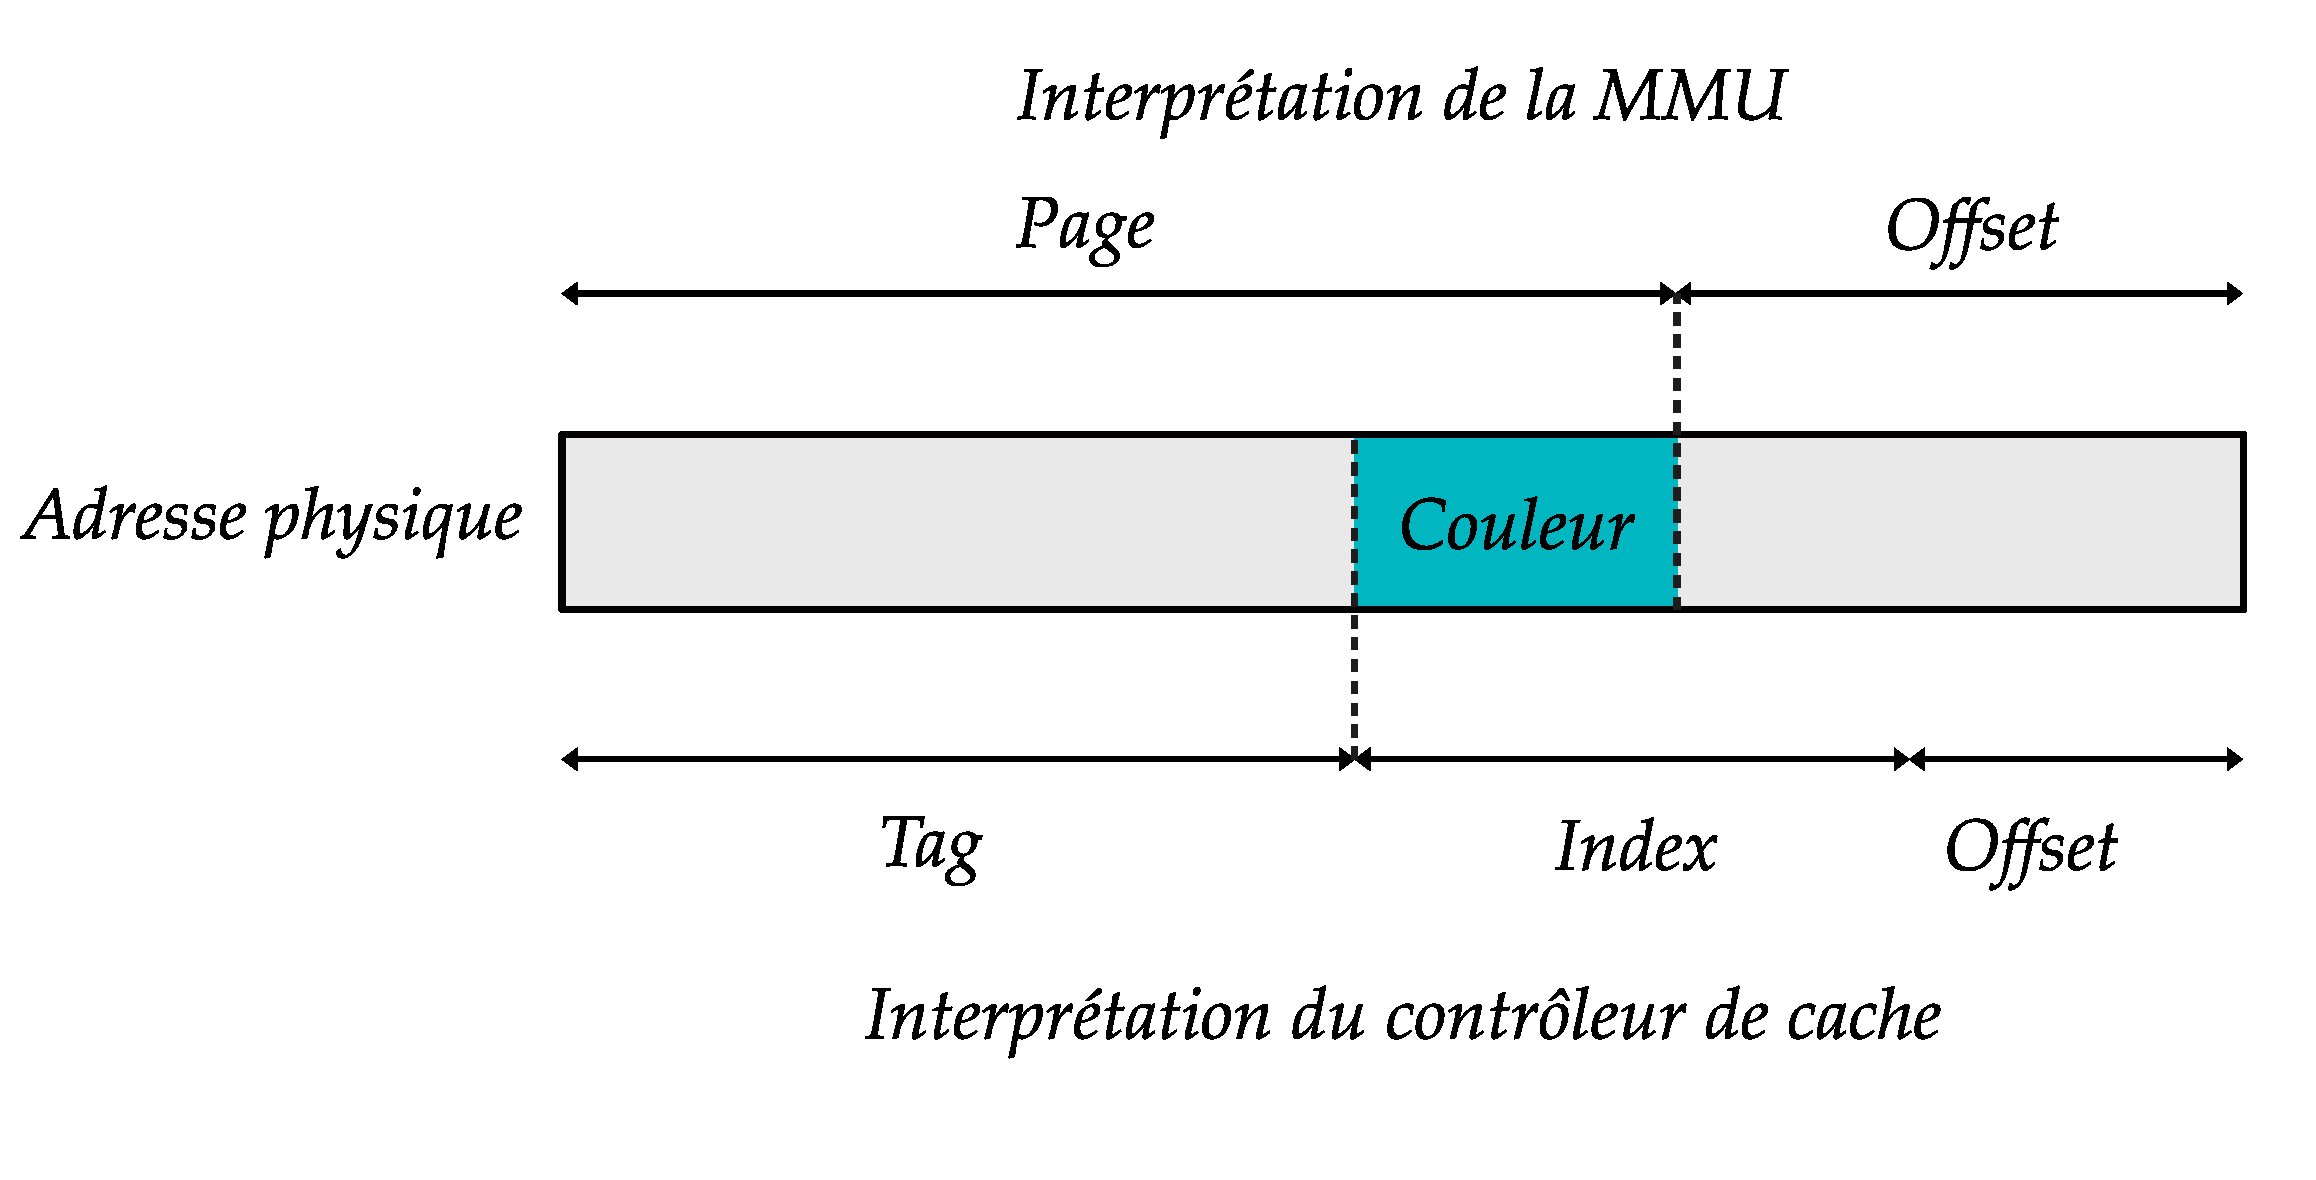
\includegraphics[width=0.65\linewidth]{graphics/figures/coloring.pdf}
	\caption{\label{fig:coloring}Bits de couleurs utilisés pour la coloration de cache}
\end{figure}

%Coloration de page. Technique logiciel. Association page virtuelle page physique. Encodage couleur dans addresse physiques. bits de pages. Utilisé en mono-coeur pour optimiser les caches. En multi-coeur permet de partitionner le cache en attribuant des couleurs disjointes entre les différents coeurs. Extension à d'autres types de ressources.

En pratique, l'application de la coloration de page se heurte à plusieurs difficultés.
Tout d'abord, pour utiliser cette technique il faut savoir comment les adresses sont interprétées par les différents composants que l'on souhaite partitionner.
Cette information n'est pas toujours disponible.
Des approches de rétro-ingénierie~\cite{yun2014palloc,panchamukhi_providing_2015} ont néanmoins été proposées pour pallier ce manque d'information.
Elles se basent sur l'étude du temps de réponse d'accès mémoire en fonction des adresses accédées.
L'arrivée des fonctions de hachages pour indexer les caches pose de nouveaux problèmes à la mise en œuvre de la coloration de cache.
Ces fonctions transparentes pour l'utilisateur ont une influence non négligeable sur les performances.
Ainsi, elles constituent souvent un secret industriel et doivent être identifiées par rétro-ingénierie~\cite{yarom2015mapping}.
De plus, même en connaissant la fonction de hachage, il n'est à connaissance pas possible de colorer des caches indexés de la sorte.

La coloration de pages est un mécanisme nécessitant du support au niveau de l'allocateur de pages physiques du système d'exploitation.
Or, ce mécanisme a des inconvénients pouvant dissuader les développeurs de systèmes d'exploitation d'implanter le support nécessaire à sa mise en œuvre.
C'est par exemple le cas dans le noyau \textsc{Linux}~\cite{torvald2003coloring}.
Les raisons invoquées sont une allocation de pages physiques rendue plus complexe et de possibles augmentations de la pression mémoire~\footnote{Zhang et al. ont montré que ce dernier point pouvait être évité en n'employant la coloration que sur les pages les plus utilisées~\cite{zhang2009towards}. Bien que prometteuse, cette solution rend d'autant plus complexe l'allocation de page physique.}.
Pour employer la coloration de pages sur ces systèmes, il faut donc utiliser un allocateur de pages spécifique.
À cette fin, Yun et al. ont proposé \textsc{PALLOC}~\cite{yun2014palloc}, un allocateur de page pour \textsc{Linux} gérant la coloration de pages.


% Elle rends l'allocation de pages physiques plus complexes, et peut augmenter la pression mémoire (bien que Zhang et al. ont montré que ce problème pouvait être contourné en utilisant la coloration que sur les pages les plus utilisées~\cite{zhang2009towards}).
% Pour ces raisons, elle n'est pas implantées dans tout les systèmes d'exploitation, notamment Linux~\cite{torvald2003coloring}.
% Pour supporter la coloration de page sous Linux, il faut donc passer par un allocateur de page spécifique comme PALLOC~\cite{yun2014palloc}.

%Nécessite de connaitre le mapping. Pas toujours possible. Notamment avec fonction de hachage pour indexation. Support OS pour coloration pas toujours disponible. Complexifie allocation de page physique. Augmentation de la pression mémoire. PALLOC réponse aux deux problèmes. Allocateur de page pour linux. Détection des mappings addresse matériel.
\paragraph{Support matériel}

Certaines architectures offrent du support matériel pour l'isolation spatiale, notamment dans les caches avec les fonctionnalités de verrouillage de lignes et de verrouillage de voies.
Le verrouillage de lignes permet de protéger spécifiquement une donnée.
Tandis que le verrouillage par voie permet d'empêcher la sélection de certaines voies par l'algorithme de remplacement.
Cette dernière méthode est généralement préférée, dans la mesure où elle ne nécessite pas de spécifier quelles données sont verrouillées.
Le verrouillage de voies peut être utilisé conjointement à la coloration de page afin de permettre un partitionnement à la granularité d'une page~\cite{mancuso2013real}.

\subsubsection{Conclusions}

Dans les systèmes temps-réel, le gain de déterminisme apporté par l'isolation spatiale a des avantages, en permettant par exemple de simplifier certaines analyses, mais aussi des inconvénients. 
L'isolation spatiale apporte un gain de déterminisme qui peut être coûteux en termes de performance en isolation.
Ce compromis a été étudié par Kim et al.~\cite{kim2017attacking} et Blin et al.~\cite{blin2016maximizing}, qui ont tous les deux conclu à de meilleures performances avec l'isolation spatiale.
Un autre problème est la gestion des couleurs au sein du système.
À cet effet, Ward et al. propose de considérer les couleurs comme des ressources partagées.
Et propose une analyse d'ordonnancement associée, se basant sur le principe d'équivalence avec un système mono-cœur~\cite{ward2013outstanding}.


%Support matériel. Verrouillage par ligne et par voies. Par ligne, verrouillage explicite des données. Par voie, plus utilisé. Permet de désigner les voies utilisés dans la politique de remplacement du cache. Utilisation conjointe avec la coloration de page permet une bonne granularité.

% Partitionement en temps réel. Gain de déterminisme vs perte de performance. Support des couleurs WARD. limité au cache. ANalyse d'ordonancement en considérant couleurs comme ressource partagée.
% Analyses font des hypothèse. En particulier sur la DRAM.

\subsubsection{Isolation temporelle}

L'isolation temporelle a pour but d'empêcher l'accès simultané à une ressource, en allouant des fenêtres de temps à chaque cœur (polititque TDMA~\footnote{Time Division Multiple Access}).
Nous ne parlerons ici que des méthodes logicielles, que l'on peut qualifier de méthodes de contrôle~\cite{girbal2015deterministic}.

% Approche de controle selon Girbal et al. Mise en oeuvre de politique TDMA en logiciel. Plus dur à mettre en oeuvre efficacement qu'isolation spatiale.

Une première approche de contrôle est l'approche tout ou rien, illustrée dans la figure~\ref{fig:tout_ou_rien}.
Celle-ci s'applique dans les systèmes à criticité mixte~\cite{vestal2007preemptive}, dans lesquels des tâches non critiques peuvent être soumises à des interférences (les tâches $PR1, PR3, PR4$ de la figure~\ref{fig:tout_ou_rien}) et des tâches critiques doivent absolument être isolées (la tâche $PR2$).
Cette approche peut être décrite par la règle suivante:
\begin{enumerate}
	\item Si une tâche critique est ordonnancée sur un cœur, les tâches de tous les autres cœurs doivent être suspendues.
	\item Lorsque des tâches non critiques s'exécutent, les tâches critiques sont suspendues.
\end{enumerate}
Ainsi, on peut s'assurer que les tâches critiques ne souffrent pas d'interférences.
Cette approche a notamment été utilisée dans l'hyperviseur temps-réel \textsc{PikeOS} \textsc~\cite{pikeOS} pour obtenir , sur un processeur bi-cœur, le plus haut niveau de certification dans un contexte ferroviaire~\cite{fisher2013certifying}.
%Bien qu'offrant une isolation parfaite à l'application temps-réel, cette approche est aussi très inefficace car elle ne permet d'exploiter qu'un seul coeur à la fois pour l'exécution  d'applications critiques.

% Par l'ordonancement. Criticité mixte. Application non critique peuvent subir des interférences. Pas les applications critiques. Application critique exécutée en isolation => applications non critique suspendues. Utilisé par PikeOS. A permis certification dans le ferroviaire pour un bi-coeur. Inneficace.

\begin{figure}
	\centering
	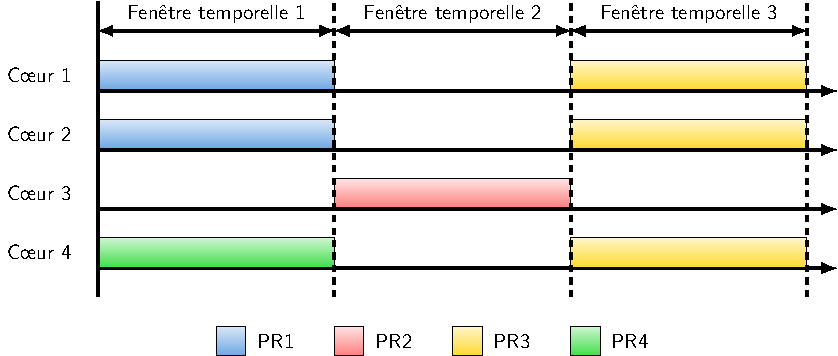
\includegraphics[width=\linewidth]{graphics/figures/tout_rien.pdf}
	\caption{\label{fig:tout_ou_rien}Ordonnancement tout ou rien}
\end{figure}

Si elle offre une isolation parfaite aux applications critiques, la solution employée dans \textsc{PikeOS} ne permet pas aux applications critiques de bénéficier du parallélisme.
Une meilleure utilisation des ressources est possible en faisant des hypothèses sur l'exécution des tâches.
Des modèles d'exécution, comme le superblock~\cite{durrieu2014predictable,schranzhofer2011timing}, ou PREM~\cite{pellizzoni2011predictable} permettent de diviser les applications en phases de communication et en phases d'exécutions.
Durant les phases de communications, l'application peut utiliser des ressources partagées.
Tandis que dans les phases d'exécution, l'application n'utilise que des ressources locales à un cœur.
Un ordonnancement des différentes phases est ensuite effectué, en permettant l'exécution en parallèle des phases d'exécutions et en s'assurant de l'exécution séquentielle des phases de communications (figure~\ref{fig:prem}).
Ce type de modèle a été utilisé dans de multiples travaux sur l'ordonnancement dit \emph{memory centric}~\cite{yao2012memory,2012_bak_memory,2014_alhammad_schedulability}.
Rivas et al.~\cite{rivas2019implementation} détaillent l'implantation du support pour le modèle PREM, dans le système d'exploitation temps-réel multi-cœur Hiperros~\cite{hipperos}~\cite{rivas2019implementation}.
Ce type de modèle permet d'améliorer la granularité de l'isolation temporelle, en permettant le parallélisme sur les phases d'exécutions.
Il nécessite par contre des adaptations du logiciel, rendant ce type d'approche incompatible avec des logiciels patrimoniaux.

%Modèle d'exécution. Superblock, ou PREM. Division de l'application en phases. Distinction entre phases d'exécution et de communications.Phase d'exécution utilise des ressources locales. Phases de communication utilise la mémoire.Ordonancement des phases d'exécution en parallèle. Ordonancement séquentiel des phases de communication. Plus efficace que l'approche tout ou rien. Pas compatible toutes les applications. Granularité de l'ordonancement. Sous utilisaiton du matériel malgré tout.

\begin{figure}
	\centering
	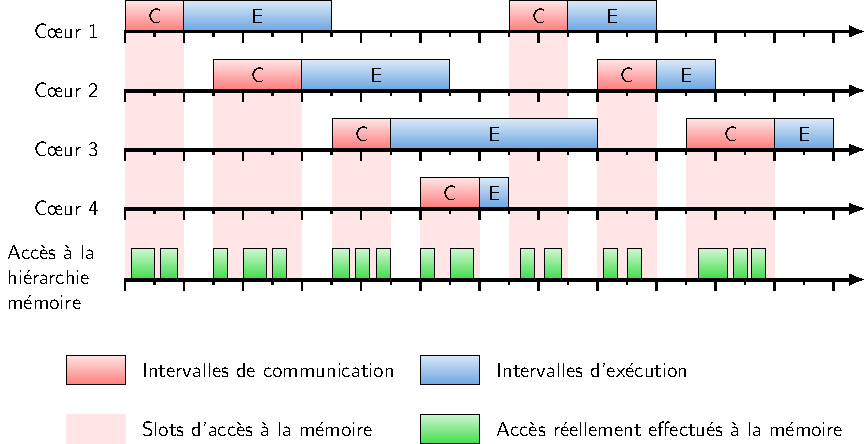
\includegraphics[width=\linewidth]{graphics/figures/prem.pdf}
	\caption{\label{fig:prem}Ordonnancement d'une tâche avec un modèle d'exécution déterministe}
\end{figure}

\textsc{MARTHy}~\cite{jean2015hypervisor} est un logiciel de contrôle permettant de mettre en œuvre une politique d'accès TDMA vers la mémoire dans un hyperviseur.
Le contrôle des accès est réalisé à l'aide d'une stratégie de programmation de la MMU et de fonctionnalités de verrouillage de cache.
L'idée est de maintenir l'invariant que toute page disposant d'une traduction valide est présente et verrouillée dans le cache.
Lorsqu'une application tente d'accéder à une donnée qui n'est pas présente en cache, une interruption de défaut de page est levée:
\begin{enumerate}
	\item Une exception de défaut de page est levée, donnant ainsi la main à l'hyperviseur (Marthy).
	\item Un emplacement pour accueillir la page à charger est sélectionné. 
	Dans la majeure partie des cas, cette étape consiste à sélectionner une page à évincer.
	\item L'hyperviseur attend le début d'une fenêtre temporelle durant laquelle il est autorisé à accéder à la mémoire.
	\item La page est chargée durant la fenêtre.
\end{enumerate}

\textsc{MARTHy} permet donc de bénéficier des avantages apportés par les modèles d'exécutions déterministes sur tout type d'application.
Cette approche néanmoins dégrade significativement les performances lorsque le mécanisme de contrôle est très sollicité.
De plus, sa mise en œuvre nécessite des fonctionnalités de verrouillage de cache, qui ne sont pas toujours disponibles.

%Système de controle permettant d'implanter une politique TDMA.
%Maintenance de l'invariant: toute page avec une correspondance valide est présente et verrouillée en cache. Sur défaut de page attente d'une fenetre temporelle. Implantée dans PowerPC. Repose sur la possibilité de gérer TLB en soft. problème de performances.

\begin{figure}
	\centering
	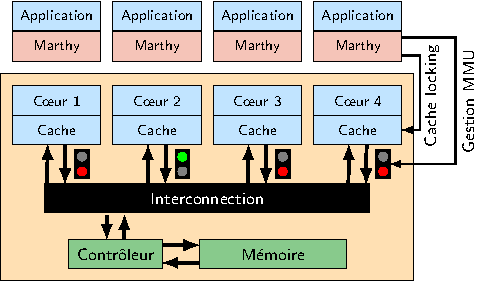
\includegraphics[width=0.75\linewidth]{graphics/figures/marthy.pdf}
	\caption{\label{fig:marthy}\textsc{MARTHy}}
\end{figure}

\subsubsection{Conclusions}

L'isolation temporelle a l'avantage d'offrir beaucoup de déterminisme en éliminant les accès simultanés aux ressources partagées.
Ce déterminisme est néanmoins acquis au prix d'une sous utilisation du matériel.
Elle s'avère néanmoins difficile à mettre en œuvre.
Les modèles d'exécutions déterministes sont une piste prometteuse pour les applications futures.
Néanmoins, il n'est pas certain que toutes les applications puissent être écrites pour satisfaire à ce genre de modèle.
Une question demeure sur la granularité du contrôle des accès.
Si une granularité plus fine peut permettre une meilleure utilisation du matériel, le coût du contrôle augmente également.
À notre connaissance, il n'y a pour le moment pas de réponse claire au problème du coût de contrôle dans la littérature.
% Isolation temporelle => Déterministe. Sous utilisation du matériel. Difficulté de mise en oeuvre.

\subsection{Systèmes de régulation}

L'isolation des différents cœurs, qu’elle soit spatiale ou temporelle, offre du déterminisme au prix d'une dégradation des performances.
Selon le niveau de charge du système, le gain de déterminisme peut ne pas justifier ce coût.
Le but des \emph{systèmes de régulation} est d'adapter le niveau d'isolation pour les tâches temps-réel en fonction de la pression effectivement exercée sur les ressources partagées.
Nous distinguons deux composants majeurs dans ces systèmes:
\begin{itemize}
	\item Un \emph{plan de données}, en charge de déterminer s’ il y a un risque de dépassement d'échéance en fonction de l'état observé du système.
	\item Un \emph{plan de contrôle}, en charge de rétablir un domaine de fonctionnement sûr en cas d'alerte du plan de données.
\end{itemize}
Ce type de solutions est plutôt adapté à des systèmes à criticité mixte, car dans ce type de systèmes des tâches non critiques peuvent être suspendues pour permettre aux taches critiques de respecter leurs échéances.

%Régulation : limiter l'impact des interférences. Deux composants: plan de données => monitorage du retards. Plan de contrôle => rétablissement d'une situation sûre. Mode dégradé. Type d'approche plutot adaptée aux systèmes à criticité mixte.

Une première approche consiste à réguler l'accès aux ressources.
C'est ce que permettent les \emph{régulateurs de bandes passantes}, tels que MRS~\cite{inam2014multi} ou MemGuard~\cite{yun2013memguard}.
Ces régulateurs fonctionnent sur le principe d'un \emph{serveur périodique}.
Chaque cœur se voit attribuer un budget d'accès autorisés sur une \emph{période de régulation}.
Les éventuels dépassements de budgets sont détectés à l'aide de \emph{compteurs de performances}.
Des compteurs de performances sont utilisés pour détecter le dépassement de budget éventuel.
En pratique, ces compteurs sont programmés pour lever une interruption lorsqu'ils sont saturés et initialisés à leur valeur maximale moins le budget alloué.
Lors d'un dépassement de budget, le cœur concerné est mis en attente jusqu'à la période de régulation suivante.

Ce type d'approche peut être utilisée pour simplifier l'analyse d'ordonnancement d'un système~\cite{pellizzoni2016memory,agrawal2017contention}.
La mise en œuvre d'un régulateur de bande passante dépend directement des événements observables sur le matériel utilisé.
Notons que cette observation doit se faire indépendamment pour chaque cœur.
Ce n'est pas toujours possible sur les cibles COTS.
En effet, dans ces dernières, les ressources partagées ne sont généralement observables qu'au moyen d'un compteur global ne permettant pas de différencier la consommation des différents cœurs.

De plus, le bon fonctionnement de ce type d'approche dépend directement du dimensionnement du système et donc des budgets alloués aux différents cœurs.
En particulier, il n'y a pas de notion de sensibilité.
C'est-à-dire que si le dimensionnement du système est trop optimiste, rien ne garantit le respect des échéances temporelles.
MemGuard apporte une solution à ce problème en définissant un seuil maximal d'utilisation du bus mémoire permettant de garantir le respect des échéances, ce qui pose un problème de sous utilisation des ressources.

%La régulation en tant que telle nécessite donc de sous-utiliser les ressources pour être sure.

%Régulation de bande passante. Permet de limiter l'aggressivité des applications. MemGuard et MRS.Principe d'un serveur périodique. Chaque coeur a un budget de consommation: nombre d'accès max par période. Budget renouvelée au début de chaque periode de régulation. Consommation mémoire mesurée avec compteur de performances. Exceptions levée sur overflow. Quand exception suspension des taches sur le coeur jusqu'à la prochaine période de régulation. Nécessite d'avoir les évenements pertinents. Pas de notion de sensibilité. Plus d'interférences -> Moins de consommation.MemGuard utilise un seuil global. Sous utilisation. Utilisé par certaine études WCET.

\begin{figure}
	\centering
	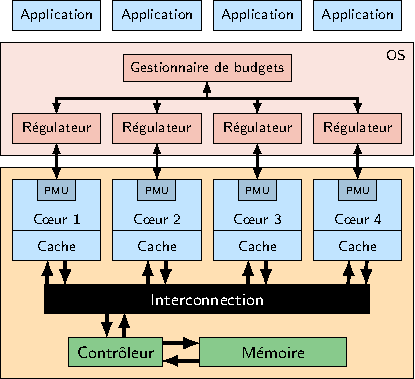
\includegraphics[width=0.6\linewidth]{graphics/figures/memguard.pdf}
	\caption{\label{fig:memguard}MemGuard}
\end{figure}

Le \emph{Contrôleur de WCET distribué}~\cite{kritikakou2014run,kritikakou2014distributed} est une approche de régulation dont le plan de contrôle n'est pas focalisé sur l'utilisation des ressources, mais sur le retard pris par les tâches temps-réel.
Cette approche concerne les systèmes à criticité mixte.
Des \emph{points de contrôles} sont injectés dans les applications temps-réel du système.
Ces points de contrôle comprennent une \emph{condition de sûreté} permettant de vérifier que la tâche peut respecter ses échéances malgré la contention.
Si la condition de sûreté d'un point de contrôle n'est pas respectée, alors une notification est envoyée à un \emph{contrôleur de WCET} qui en réponse va suspendre les tâches non critiques du système.
La principale difficulté dans la mise en œuvre de ce type d'approche est le placement des points de contrôles et la spécification des conditions de sûreté.
% Lorsqu'ils sont exécutés, ces points de contrôle vériefie une \emph{condition de sureté} et notifie un \emph{contrôleur de WCET} si celle 

%Distributed WCET controler. Solutions pour système à criticité mixte. Injection de points de contrôles dans le code des applications. Point de contrôles s'assure du respect des échéances temporelles. Si condition de sureté non remplie, tâches non critiques suspendues. Pb placements des points et validité des conditions de sureté. 

\begin{figure}
	\centering
	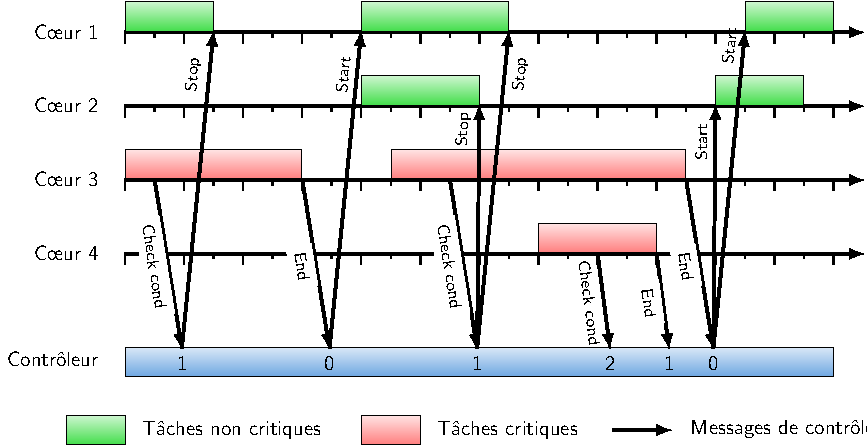
\includegraphics[width=\linewidth]{graphics/figures/kri.pdf}
	\caption{\label{fig:kritikakou}Contrôleur de WCET distribué}
\end{figure}

La solution proposée par Blin et al.~\cite{blin2016maximizing} vise à maintenir le retard subi par une application en dessous d'un seuil déterminé lors de la conception du système.
Tout comme le contrôleur de WCET distribué, cette approche s'applique à des systèmes à criticité mixte et suspend les tâches non critiques lorsque le seuil de retard spécifié est atteint.
Ce mécanisme n'exige pas compteurs locaux, mais un compteur global, la rendant compatible avec la plupart des cibles COTS.
Elle est néanmoins limitée au cas où seul un cœur exécute des applications temps-réels.
Ce système repose sur trois grandes étapes. Deux étapes hors-ligne permettent de définir le plan de données, tandis que la troisième étape en ligne implante le plan de contrôle:
\begin{enumerate}
	\item \emph{Modèle de retards de la plateforme matérielle}. Cette étape consiste à définir une fonction, permettant d'associer un surcoût temporel à une consommation de bande passante en isolation et une bande passante globale observée.
	Cette fonction est conservative et construite à partir de données expérimentales.
	De multiples expériences sont effectuées avec des microbenchmarks, et seuls les cas les plus pessimistes sont retenus.
	\item \emph{Modèle de consommation de l'application à protéger}. Dans cette étape, la consommation de bande passante d'une application est mesurée en isolation.
	Les mesures sont effectuées sur différentes phases de l'application.
	\item \emph{Contrôle en ligne} À l'exécution, un mécanisme de contrôle mesure la bande globale et détermine le retard subi par l'application temps-réel en utilisant les deux modèles constituant le plan de données.
	Lorsque le retard cumulé est trop élevé, les applications non temps-réels sont suspendues.
\end{enumerate}

La mise en œuvre efficace de ce type d'approche dépend grandement de la qualité du plan de données que l'on a pu définir.
Plus le modèle de retards est imprécis, plus vite les applications non critiques sont suspendues, ce qui résulte dans une utilisation moindre du matériel.
Une meilleure précision du modèle de retards peut donc conduire à une meilleure utilisation du matériel.

\subsubsection{Conclusions}

Les systèmes de régulation permettent d'adapter le niveau d'isolation du système en fonction de l'utilisation globale des ressources matérielles.
Ces approches offrent donc un compromis entre déterminisme et efficacité, ce qui les rend particulièrement attractives pour des applications industrielles.
L'implantation efficace de tel système demeure néanmoins un défi important.
Un verrou technologique important réside notamment dans le plan de données en charge de détecter les situations à risque.
En effet, pouvoir détecter précisément ces situations détermine directement la confiance que l'on peut avoir dans ces approches et éviter les surdimensionnements excessifs.

% Régulation permet de fournir un filet de sécurité. Plutot adapté à des système à criticité mixte où on peut mettre en place un mode dégradé.
% Plan de donnée critique. Permet de détecter précisemment situations à risque. Dimmensionnement du système important.
\section{Conclusions du chapitre}

Nous avons dans ce chapitre présenté l'impact des interférences dans le cadre des systèmes temps-réels.
Prendre en compte les interférences lors de la conception des systèmes temps-réels revient à surdimensionner ces derniers.
En effet, le dimensionnement de ces systèmes doit correspondre aux pires cas.
La complexité et l'opacité du matériel moderne rendent ces interférences difficilement prévisibles et conduisent à des surdimensionnements inacceptablement pessimistes des systèmes.

À l'heure actuelle, les approches traditionnellement employées pour l'analyse de pire temps d'exécutions sont mises en échec par le problème des interférences.
Il est possible dans certains cas d'améliorer l'isolation des différents, mais cela se fait au détriment des performances.
Enfin, des approches de régulation permettent d'obtenir un compromis intéressant entre déterminisme et performances, mais leur mise en œuvre nécessite d'anticiper efficacement le retard subi à cause des interférences.

Dans le reste de ce document, nous présentons nos travaux dont le but est de caractériser la sensibilité aux interférences des applications à partir d'une caractérisation de leur comportement exécutée seules.
Le but est de pouvoir estimer à priori le retard que peut subir un programme, mais aussi de permettre, à terme, la conception de 
systèmes de régulation efficaces.
% Autre approche proposée par Blin et al. Meme principe que Kritikakou. Condition de sureté basés sur la consommmation. 3 étape deux hors ligne, 1 en ligne. Caractérisation de la consommation mémoire. Modèle de retards. \cleardoublepage

\part{Contributions}

% !TEX root = ../main.tex

\chapter{\label{chapitre:evaluer_impact}Évaluer l'impact des interférences mémoires}

%\minitoc

%In this section, we present a methodology to study the impact of interferences on a given hardware platform.
%First we present a set of microbenchmarks that cover a wide range of memory behavior.
%Then we describe the experimental platform used in this article.
%This is followed by a description of our interference measurement protocol.
%Finally, we evaluate the range of sensitivity covered by our microbenchmarks.

Dans ce chapitre, nous nous penchons sur l'étude empirique de l'ampleur du phénomène d'interférences sur une carte multi-cœur COTS.
Cette étude a non seulement pour but de déterminer l'impact des ralentissements subis, mais également à quel point ces ralentissements peuvent varier.
Cela pose deux difficultés auxquelles nous allons apporter des solutions dans ce chapitre.
La première étant d'identifier les aspects pertinents du trafic mémoire pour le problème d'interférences. 
La seconde est d'avoir un ensemble d'applications représentatives de ces différents aspects.

Ce chapitre est organisé en trois sections.
Dans la première section, nous présenterons la plateforme matérielle de référence sur laquelle nous conduirons le reste de nos travaux.
Dans la deuxième section, nous présenterons un modèle événementiel nous permettant d'identifier différents aspects du comportement d'accès à la mémoire d'un programme.
Nous introduirons, dans la section suivante, un ensemble de microbenchmarks paramétrables permettant de générer différents types de trafic.
Enfin, dans la quatrième section, nous utiliserons ces microbenchmarks pour étudier l'impact des interférences sur notre matériel de référence.

% !TEX root = ../main.tex

\section{Plateforme matérielle}
\label{section:plateforme_materielle}

    Dans cette section, nous allons détailler la carte que nous avons utilisée pour effectuer nos travaux en portant une attention particulière sur la hiérarchie mémoire.

    % Ressources en ligne :
    %
    % i.MX6 DDR3 RAM-Performance 32 bit vs. 64 bit interface.
    %     https://community.nxp.com/thread/329671
    %
    % i.MX6 - question about DDR memory bandwidth utilization
    %     https://community.nxp.com/thread/320997
    %
    % https://community.arm.com/thread/8295
    %     https://community.arm.com/thread/8295
    %
    % What is AXi?
    %     https://www.youtube.com/watch?v=0Dt8rWJdiJo
    %
    % Migrating from AHB to AXI based SoC Designs
    %     https://www.doulos.com/knowhow/arm/Migrating_from_AHB_to_AXI/
    %
    % Introduction to AXI
    %     http://www.analyticsengines.com/developer-blog/introduction-to-axi/
    %
    % Why is the I-cache designed as VIPT, while the D-cache as PIPT?
    %     https://community.arm.com/thread/5874
    %
    % Line Fill Buffers
    %     https://docs.google.com/presentation/d/1b-woFnas1HL5e4nkbyFAPjTrd884pBG98etEEjqSO_o/edit#slide=id.g20269671_3_105

%     \itodo{
%         Attributs du cache :
%         \begin{itemize}
%             \item Taille d'une ligne de cache
%             \item Taille d'un mot mémoire
%             \item Cache associatif : niveaux d'associativité
%             \item Politique de remplacement des données
%             \item Politique d'écriture utilisée
%             \item Politique d'allocation utilisée
%             \item Indexation du cache : avantages et inconvénients
%             \item Tampons utilisés
%         \end{itemize}
%   }

    Nous utilisons une carte i.MX6Q Sabre Lite comme plateforme matérielle de référence pour nos travaux.
    Ce choix est motivé par plusieurs raisons.
    Tout d'abord, nos travaux s'inscrivant dans le cadre d'une thèse CIFRE, le matériel choisi se devait d'être représentatif de celui utilisé dans l'industrie.
    C'est le cas de cette carte, initialement conçue pour des applications multimédias.
    Une variante automobile~\cite{manuel:i_MX_6Dual_6Quad_automotive_and_infotainment_applications_processors} de cette carte a d'ailleurs été largement utilisée par un grand nombre de fabricants et de fournisseurs de l'industrie automobile.
    La deuxième raison qui motive notre choix est que cette carte offre un bon niveau de documentation.

    % Nos travaux s'inscrivant dans le cadre d'une thèse CIFRE, le matériel de référence que nous utilisons se devait d'être représentatif de celui utilisés en contexte industriel.
    % Notre choix s'est porté sur la carte embarqué i.MX6 SABRE Lite~\cite{sabrelite}.
    % Il s'agit d'une carte de développement à bas coût, initialement prévue pour exécuter des applications multimédia en utilisant les systèmes d'exploitation Linux et Android.
    % Notons qu’il existe une variante automobile de cette plate-forme (SABRE Automotive \cite{manuel:i_MX_6Dual_6Quad_automotive_and_infotainment_applications_processors}) qui a largement été utilisée par un grand nombre de fabricants et de fournisseurs du monde automobile.

    \begin{figure}[!ht]
        \centering
        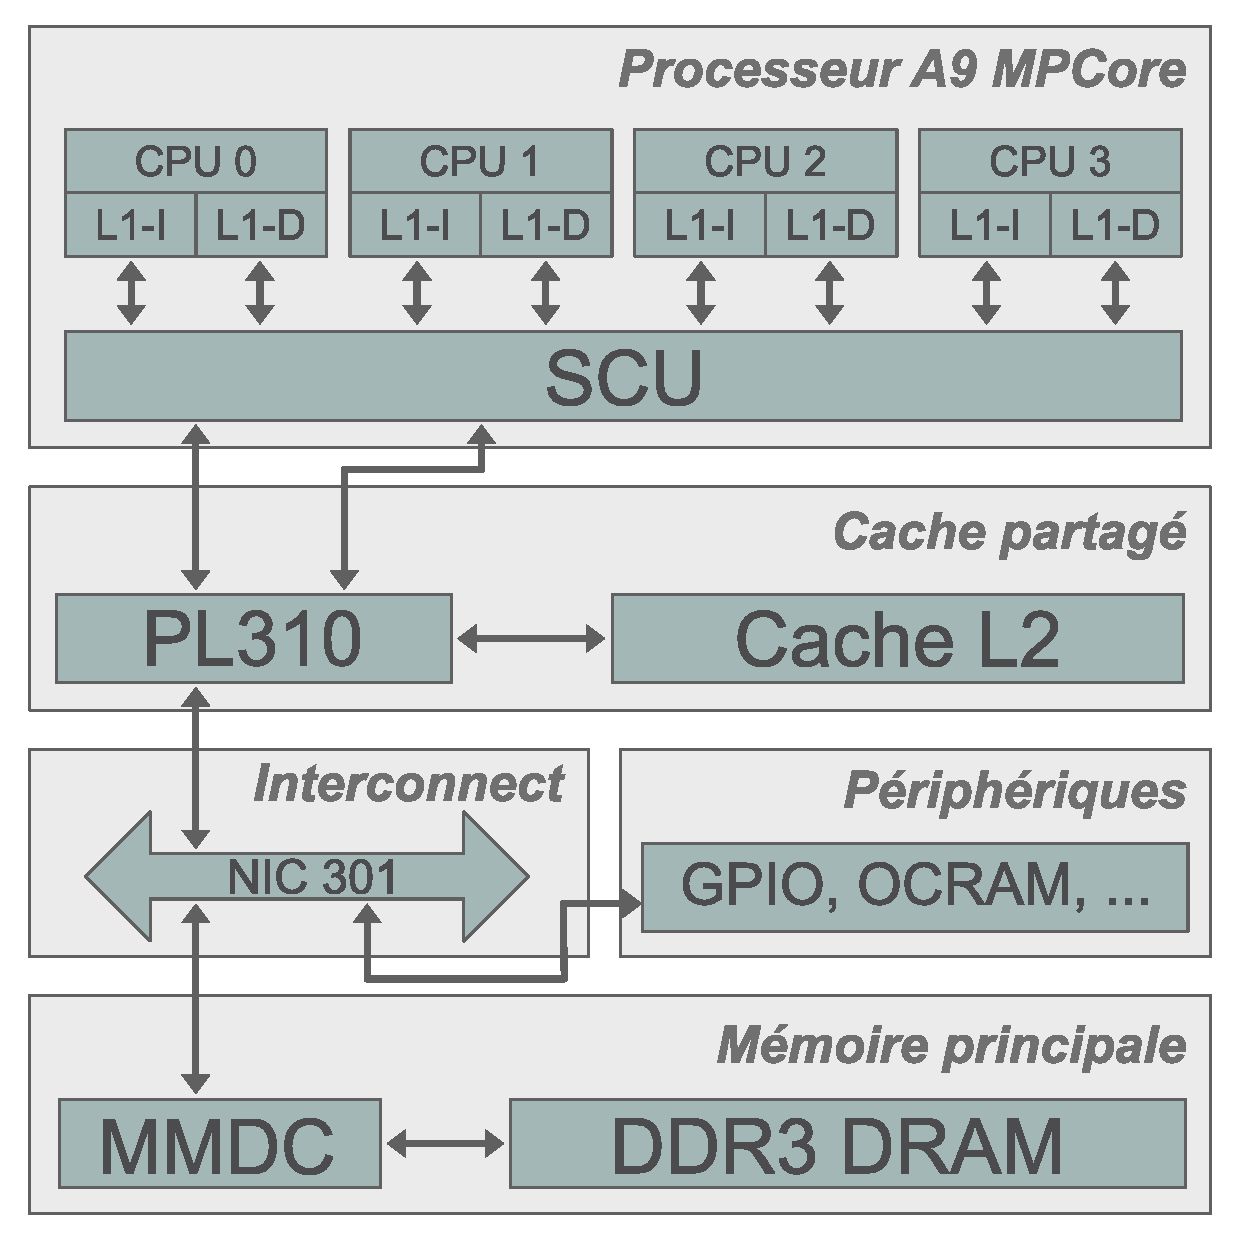
\includegraphics[width=0.5\linewidth]{sabrelite-block-diagram}
        \caption{Architecture matérielle simplifiée de la carte SABRE Lite}
        \label{fig:archiIMX6}
    \end{figure}

    L'unité de calcul de la carte est composée d'un processeur \emph{i.MX 6}, basé sur un quatre-cœurs \emph{Cortex A9 MPCore}, connecté à un cache L2 externe \emph{PL310} d'un mégaoctet. Le contrôleur mémoire \emph{MMDC} qui gère l'accès à un gibioctet de mémoire DDR3 est connecté à un bus d'interconnexion \emph{NIC-301} qui assure la connexion entre les consommateurs de mémoire (Processeur, GPU …) et différents périphériques (PCIe, MMDC, OCRAM, ...).

    L'ensemble des composants sont reliés par des bus \emph{AXI} (\emph{AMBA eXtensible Interface}) un standard développé par ARM qui effectue une liaison point à point pour relier deux modules matériels. Un module maître amorce une transaction de données en lecture ou en écriture vers un module esclave qui reçoit et répond à la transaction. L'ensemble de ces bus est équipé de deux canaux séparés qui permettent de traiter les transactions en lecture en parallèle de celles en écriture.
    %http://www.design-reuse.com/articles/24123/amba-ahb-to-axi-bus-comparison.html)

    %La figure \ref{fig:archiIMX6} affiche une vue d'ensemble simplifiée de la plate-forme i.MX 6 SABRE Lite.

    Nous allons maintenant, nous appuyer sur la vue d'ensemble de l'architecture de notre plateforme, présentée dans la figure \ref{fig:archiIMX6}, pour détailler plus précisément les composants matériels utilisés dans nos travaux. Nous allons, dans une première partie, effectuer une description du processeur implanté au sein de notre carte pour ensuite, dans les parties suivantes, étudier les différents niveaux de hiérarchie mémoire, matérialisés par les caches L1, le cache L2 et le contrôleur mémoire, qui sont partagés entre les cœurs et les périphériques matériels.

%    \FloatBarrier

    %\subsection{Processeur cortex-A9 MPCore}
    \subsection{Processeur}

        Le processeur de notre carte est composé de quatre cœurs \emph{cortex-A9} regroupés ensemble au sein d'un unique circuit intégré intitulé \emph{Cortex-A9 MPCore}.

        \subsubsection{Cœur cortex-A9}

            % === 12.3 Platform configuration ===
            %
            % --- Cortex-A9 Core configuration ---
            %
            %     DCACHESIZE              32      L1 Data cache size
            %     ICACHESIZE              32      L1 Instruction cache size
            %     TLBSIZE                 128     JAZELLE_PRESENT Yes Providing ARM's Jazelle technology hardware extensions.
            %     FPU_PRESENT             No      The FPU functions are provided by NEON, thus additional FPU cannot be used.
            %     NEON_PRESENT            Yes     Use MPE, NEON Co-Processor and FPU
            %     PRELOAD_ENGINE_PRESENT  No      May only be beneficial in Video processing.
            %
            %     Chapter 1 Introduction
            %     1.1 About the Cortex-A9 processor
            %
            % The Cortex-A9 processor is a high-performance, low-power, ARM macrocell with an L1 cache subsystem that provides full virtual memory capabilities. The Cortex-A9 processor implements the ARMv7-A architecture and runs 32-bit ARM instructions, 16-bit and 32-bit Thumb instructions, and 8-bit Java bytecodes in Jazelle state.
            %
            % 1.5 Interfaces
            %     The processor has the following external interfaces:
            %         AMBA AXI interfaces
            %         Debug v7 compliant interface, including a debug APBv3 external debug interface
            %         DFT.
            %     For more information on these interfaces see:
            %         AMBA AXI Protocol Specification
            %         CoreSight Architecture Specification
            %         Cortex-A9 MBIST Controller Technical Reference Manual
            %
            % Chapter 2 Functional Description
            %     2.2 Interfaces
            %     2.4 Power management
            %
            % Chapter 7 Level 1 Memory System
            %
            % Chapter 11 Performance Monitoring Unit

            L'unité de calcul \emph{Cortex-A9}, présentée dans la figure \ref{fig:cortex_A9_uniprocessor_system}, est un processeur à haute performance et à faible consommation conçu par la société ARM suivant l'architecture \emph{ARMv7-A} \cite{manuel:ARMv7} et les jeux d'instructions 32-bit ARM, 16-bit et 32-bit Thumb \cite{manuel:cortex_A9_technical_reference_manual}.

            \begin{figure}[!ht]
                \centering
                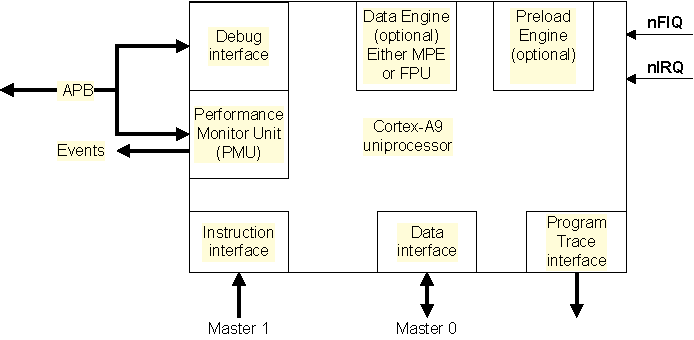
\includegraphics[width=0.9\linewidth]{cortex_A9_uniprocessor_system}
                \caption{Système monoprocesseur Cortex-A9 \cite{manuel:cortex_A9_technical_reference_manual}}
                \label{fig:cortex_A9_uniprocessor_system}
            \end{figure}

            Chaque processeur possède une unité de mesure des performances (\emph{Performance Monitoring Unit}) qui contient sept compteurs matériels pouvant être utilisés aussi bien pour récupérer des statistiques sur les opérations exécutées par le processeur (Nombre de cycles …) que sur les accès réalisés par le système mémoire (Cache L1 MISS, Cache L1 HIT, ...). Un des compteurs est configuré en dur pour compter le nombre de cycles effectués par le processeur tandis que les six compteurs restants peuvent être configurés pour enregistrer un des 58 événements mesurables.
            Nous utiliserons ces compteurs pour caractériser en partie le comportement des applications.



        \subsubsection{Processeur cortex-A9 MPCore}

            % Chapter 12 ARM Cortex A9 MPCore Platform (ARM)
            %
            % 12.3.1 Platform and SCU configuration \cite{i.MX_6Dual_6_Quad_Applications_Processor_Reference_Manual}
            % Table 12-3. Cortex-A9 configuration
            %
            % Option                  Selected    Value Comments
            % MP_MODE                 Yes         Multi-Processor mode
            % POWER_DOMAIN_WRAPPER    No          Wrappers to support power off of individual cores.
            % PTM_INTERFACE_PRESENT   Yes         Use PTM as part of Trace/Debug logic.
            % PARITY                  Yes         Using RAM arrays which support parity.
            % CORE_NUM                2/4         1 Number of cores
            % INT_NUM                 128         Number of interrupts (SPIs) in GIC
            % ACP_PRESENT             No          Accelerator Coherency Port (ACP)
            % MASTER_NUM              2           Number of 64-bit AXI output master ports.

            Le processeur Cortex-A9 MPCore, présenté dans la figure \ref{fig:example_multiprocessor_configuration}, est constitué d'un ensemble de quatre processeurs Cortex A9 regroupés et connectés à une unité de contrôle nommée \emph{Snoop Control unit}.

            \begin{figure}[!ht]
                \centering
                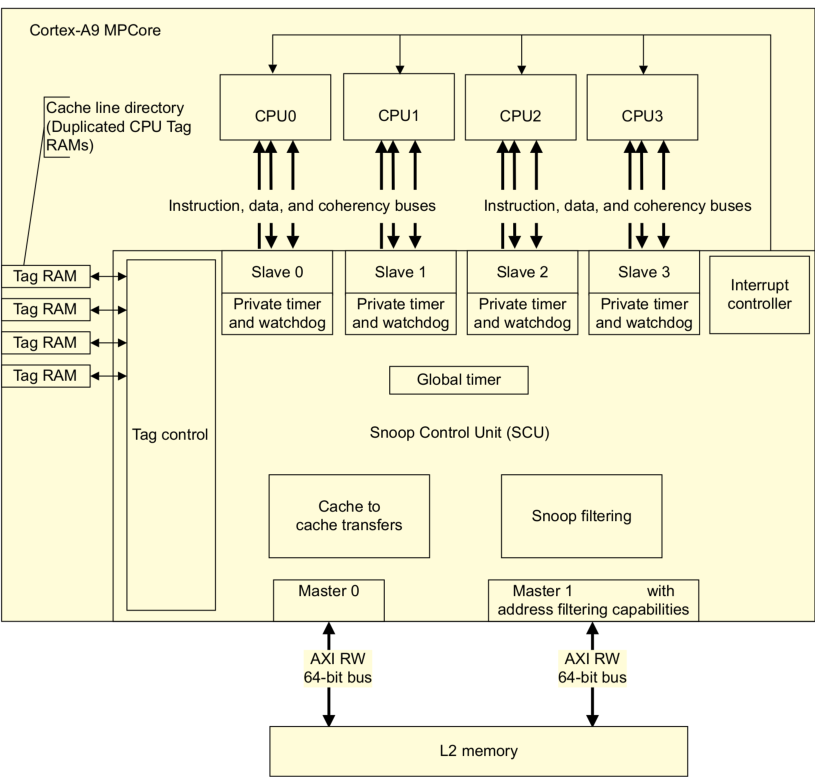
\includegraphics[width=\linewidth]{example_multiprocessor_configuration_2}
                 \caption{Exemple de configuration multiprocesseur \cite{manuel:cortex_a9_mpcore_trm}}
                 \label{fig:example_multiprocessor_configuration}
             \end{figure}
% 
            La SCU maintient la cohérence entre les caches des différents processeurs du groupe en utilisant un protocole dérivé de \emph{MESI}. Elle arbitre également les requêtes émises par les processeurs vers les niveaux de hiérarchie mémoire supérieurs et génère les accès mémoire correspondants.

            Le processeur Cortex-A9 MPCore contient un ensemble de périphériques mappés en mémoire incluant un temporisateur global, ainsi qu'un \emph{watchdog} et un temporisateur privé pour chacun des processeurs du groupe.
            %
            Un contrôleur d'interruptions respectant l'architecture \emph{Generic Interrupt Controller} \cite{manuel:gic} est également présent. Localisé, au sein du processeur MPCore, il a pour rôle de centraliser toutes les sources d'interruptions avant de les répartir vers les processeurs individuels.

            Le processeur Cortex-A9 MPCore est connecté à un contrôleur de cache externe de type PL310 de niveau 2 par deux bus AXI 64 bits et peut, théoriquement, générer (\emph{maître}) jusqu'à 24 transactions par processeur vers le cache L2 (\emph{esclave}).
            % Cortex A* MPCORe AXI issuing capabilities
            % http://infocenter.arm.com/help/index.jsp?topic=/com.arm.doc.dui0305c/Cbaifdib.html
            %
            % L2 Prefetch Hint feature}
            %\optionnel{Pour augmenter les performances du système le cœur est doté d'une unité désactivable de préchargement qui détecte les patterns de chargement mémoire réguliers et envoie des requêtes au contrôleur PL310 pour précharger des lignes de mémoire dans le cache L2.}

            % Manuel Cortex-A9 TRM
            %
            % Prefetch hint to the L2 memory interface
            %
            % The Cortex-A9 processor can generate prefetch hint requests to the L2 memory controller. The prefetch hint requests are non-compliant AXI read requests generated by the Cortex-A9 processor that do not expect any data return.
            %
            % You can generate prefetch hint requests to the L2 by:
            % •   Enabling the L2 Prefetch Hint feature, bit [1] in the ACTLR. When enabled, this feature enables the Cortex-A9 processor to automatically issue L2 prefetch hint requests when it detects regular fetch patterns on a coherent memory. This feature is only triggered in a Cortex-A9 MPCore processor, and not in a uniprocessor.

            % Manuel L2C-310 TRM
            %
            % Prefetch hints
            %
            % When you configure the Cortex-A9 processor to run in SMP mode, the automatic data prefetchers, implemented in one or more CPUs, issues special read accesses to the L2C-310. See the Cortex-A9 TRM. These special reads are called Prefetch Hints. They are indicated when a device sets ARUSERSx[8] to 1. When the L2C-310 slave ports receive such prefetch hints, they do not send any data back to the Cortex-A9 processor, they allocate the targeted cache line into the L2 cache for a miss. This behavior is not compatible with AXI. When a master other than a Cortex-A9 processor drives the L2C-310 ARUSERSx[8] must be tied 0.

            % Partie 22.1 Cache coherency du cortex a series programmers guide
            % The coherency management is implemented using a MESI-based protocol,

            % MPcore manuel
            % When Address Filtering is enabled, SCU Control Register bit [1] = 1, any access that fits in the address range between the Filtering Start Address and the Filtering End Address is issued on the AXI Master port M1. All other accesses outside of this range are directed onto AXI Master port M0.This filtering rule is applied independently of the AXI request type and attributes. When Address Filtering is disabled, accesses can be issued indifferently on AXI Master port M0 or AXI Master port M1, provided that the AXI ordering rules are respected. However, in this case, locked and exclusive accesses are always issued on AXI Master port M0.

            %The Cortex-A9 MPCore processor consists of:
            %    • From one to four Cortex-A9 processors in a cluster and a Snoop Control Unit (SCU) that can be used to ensure coherency within the cluster.
            %    • A set of private memory-mapped peripherals, including a global timer, and a watchdog and private timer for each Cortex-A9 processor present in the cluster.
            %    • An integrated Interrupt Controller that is an implementation of the Generic Interrupt Controller architecture. The integrated Interrupt Controller registers are in the private memory region of the Cortex-A9 MPCore processor

            % The Interrupt Controller is a single functional unit that is located in a Cortex-A9 MPCore design. It is responsible for centralizing all interrupt sources before dispatching them to each individual Cortex-A9 processor. There is one interrupt interface per Cortex-A9 processor.

            % The Cortex-A9 MPCore L2 interface can have two 64-bit wide AXI bus masters. In a two bus master configuration there is also an option to configure address filtering.

            % Individual Cortex-A9 processors in the Cortex-A9 MPCore cluster can be implemented with their own hardware configurations.

            % The SCU connects one to four Cortex-A9 processors to the memory system through the AXI interfaces.
            % The SCU functions are to:
            %     • maintain data cache coherency between the Cortex-A9 processors
            %     • initiate L2 AXI memory accesses
            %     • arbitrate between Cortex-A9 processors requesting L2 accesses
            %     • manage ACP accesses.
            %
            % The Cortex-A9 MPCore processor consists of:
            %     • From one to four Cortex-A9 processors in a cluster and a Snoop Control Unit (SCU) that can be used to ensure coherency within the cluster.
            %     • A set of private memory-mapped peripherals, including a global timer, and a watchdog and private timer for each Cortex-A9 processor present in the cluster.
            %     • An integrated Interrupt Controller that is an implementation of the Generic Interrupt Controller architecture. The integrated Interrupt Controller registers are in the private memory region of the Cortex-A9 MPCore processor.
            %
            %
            % Snoop Control Unit (SCU), that maintains L1 data cache coherency.

        \subsubsection{Impact sur les interférences}
        \label{processeur:impacts_sur_nos_travaux}
        Bien que les cœurs Cortex-A9 sont indépendants les uns des autres, un couplage existe au travers de l'interface MPCore, et plus particulièrement la \emph{SCU}. 
        Celle-ci a deux fonctions: maintenir la cohérence des données entre les caches L1 des différents cœurs et arbitrer l'accès au cache L2.
        % Ces fonctions sont toutes les deux sources d'interférence entre les coeurs.

        Le maintien de la cohérence entre les cœurs entraîne une augmentation du nombre d'invalidations lorsque des données sont partagées.
        Il s'agit d'une forme d'interférence spatiale qui est propre aux applications utilisant le modèle SMP.
        Vu que nos travaux se concentrent sur le modèle AMP, nous ne tiendrons pas compte de ce type d'interférence.
 
        En outre, la \emph{SCU} a également pour vocation d'arbitrer les différentes requêtes émises par les cœurs vers la hiérarchie mémoire de niveau supérieur. Or, la capacité du cache à répondre en parallèle aux requêtes d'accès étant limitée, l'ordre d'émission des requêtes vers la hiérarchie mémoire de niveau supérieur fait l'objet d'une politique d'arbitrage.
        Cette politique n'est pas détaillée dans la documentation matérielle dont nous disposons.
        Il s'agit d'un problème récurrent dans les architectures COTS.

            % Enfin, il est important de noter que la présence de compteurs matériels, au sein de chacun des cœurs, permet d'avoir une mesure précise du trafic généré vers la hiérarchie mémoire partagée sans, pour autant, permettre de discriminer quels sont les différents niveaux de la hiérarchie qui sont traversés par les requêtes. Ce choix, effectué pour des raisons de coûts, et partagé par de nombreux fondeurs, pose l’un des défis de nos travaux. En effet, il sera impossible de déterminer quel cœur a effectué les accès mémoire mesurés.

        Les sections suivantes s'attachent à décrire plus en détail les caches de premier niveau qui sont intégrées dans chacun des cœurs A9 pour ensuite porter notre attention sur le cache L2 directement connecté au processeur MPCore.

    \subsection{Hiérarchie mémoire de niveau 1}

        % P74 System Control Register pour
        %     Determines if instructions can be cached at any available cache level:
        %     Enables program flow prediction:
        %     Determines if data can be cached at any available cache level:

        Le processeur Cortex A9 dispose de deux caches, séparément désactivables, de niveau 1, d'une taille de 32KiB \cite{manuel:i_MX_6Dual_6Quad_applications_processor_reference_manual,manuel:cortex_A9_technical_reference_manual}.
        Un cache est utilisé pour contenir les instructions de code, l'autre pour charger les données. La politique de correspondance utilisée dans ces deux caches est de type « partiellement associative ».
        Ainsi, chaque cache est divisé en quatre voies. La taille d'une ligne de cache étant de 32 octets soit 8 mots mémoire, chaque voie contient 256 lignes de caches.

        Le cache d'instructions et le cache de données sont reliés à la hiérarchie mémoire de niveau supérieur par deux bus distincts AXI de 64 bits de large, le bus \emph{Master 0} étant utilisé par la partie de gestion des données et le bus \emph{Master 1} par la partie gestion des instructions.
        %
        La politique de gestion des écritures (\emph{write-through} ou \emph{write-back}) et d'allocation (\emph{read-allocate} ou \emph{write-allocate}), utilisée par le cache, peut être configurée par zone mémoire soit au niveau de la MMU ou au niveau de la MPU \cite{manuel:cortex_a_series_programmer_s_guide}.
        % Partie 10.7 Memory attributes du cortex A Series Programmers guide
        % Partie B3.7 Memory region attributes du ARM Architecture Reference Manual ARM v7-A and ARM v7-R edition

        \subsubsection{Cache d'instruction}

        \paragraph{Politique d'indexation} 
        Le cache L1 d'instructions est virtuellement indexé et physiquement tagué (\emph{Virtually indexed, physically tagged}). 
        Il utilise l'adresse virtuelle (\emph{index}), émise par le processeur, pour sélectionner l'ensemble dans lequel chercher la donnée, tandis que l'adresse physique est utilisée pour déterminer si le bloc de données recherché est présent dans le cache (\emph{tag}).
        L'utilisation d'une telle politique permet de diminuer la latence d'accès au cache, une ligne de cache pouvant être recherchée dans le cache en parallèle de la traduction d'adresse. Cette politique complexifie cependant la mise en œuvre de la cohérence des données partagées entre des processus exécutés sur le même cœur, une même ligne de mémoire physique pouvant être présente à deux endroits du cache.
        Le code des programmes exécutés étant majoritairement en lecture seule, l'utilisation d'une telle politique sur le cache d'instruction n'est donc pas rédhibitoire.
            %
        \paragraph{Politique de remplacement} 
        La politique de remplacement du cache peut être, au choix, pseudo \emph{round-robin} ou \emph{pseudo-random}.
                        
        \paragraph{Optimisations} Le cache L1 est connecté à une unité désactivable de prédiction du flux d'instructions du programme qui est utilisé pour précharger en avance les instructions qui vont être exécutées.

            % Virtually indexed, physically tagged (VIPT) caches use the virtual address for the index and the physical address in the tag. The advantage over PIPT is lower latency, as the cache line can be looked up in parallel with the TLB translation, however the tag cannot be compared until the physical address is available. The advantage over VIVT is that since the tag has the physical address, the cache can detect homonyms. VIPT requires more tag bits, as the index bits no longer represent the same address.

        \subsubsection{Cache de données}

            \paragraph{Politique d'indexation}
            Le cache L1 de données est physiquement indexé et physiquement tagué (\emph{Physically indexed, physically tagged}), ce qui augmente la latence d'accès aux données, mais facilite la mise en œuvre du partage de zones mémoire entre deux processus qui utilisent le même cache, une donnée ne pouvant être présente qu'à un seul endroit du cache.
            
            \paragraph{Politique de remplacement}
            La politique de remplacement des données utilisées par le cache est fixée en dur à \emph{pseudo-random}.
            
            \paragraph{Optimisations}
            Le cache de données est également doté d'une unité de préchargement désactivable pour charger en avance les données qui vont potentiellement être utilisées.
            %
            Un tampon \emph{store buffer} est placé entre le processeur et le cache L1 pour fusionner les écritures consécutives afin de limiter le nombre de transactions effectuées depuis le cœur vers le cache. Le cache dispose, en sus, de deux tampons de remplissage (\emph{linefill buffer}) ce qui permet de servir deux caches MISS en parallèle. Un tampon d'éviction (\emph{eviction buffer}) de la taille d'une ligne de cache est également présent. Il permet au processeur de propager une ligne de cache sale vers la hiérarchie mémoire de plus haut niveau sans que ledit processeur soit bloqué le temps de la propagation.

        \subsubsection{Impacts sur les interférences}
        \label{l1:impacts_sur_nos_travaux}

        L'existence de caches de niveau un, privés à chacun des cœurs du processeur, entraîne, lorsque les données utilisées par le processeur sont déjà présentes dans les caches, une diminution du nombre de requêtes émises vers le système mémoire.
            %
        Cette baisse, d’une part, limite le nombre d'interférences, seules les requêtes émises vers le système mémoire partagé peuvent être ralenties, et d'autre part, abaisse le nombre de requêtes envoyées vers le système mémoire ce qui se traduit par une baisse de la contention.
        Si l'ensemble de l'empreinte mémoire d'une application est suffisamment faible pour être contenue dans le cache, alors le problème de contention ne se pose plus.


        Les composants matériels que sont les unités de préchargement et les tampons \emph{linefill buffer} maximisent l'utilisation du cache en préchargeant en avance les données qui vont être utilisées.
            %
        Ils permettent également de découpler, le moment où les données sont requises dans le cache, du moment où elles sont réellement demandées, amortissant ainsi les effets des interférences sur le système mémoire.
            %
        En effet, une requête mémoire demandée en avance par l'unité de préchargement et retardée à cause de la contention sur le système mémoire peut arriver à temps pour être immédiatement utilisée.
            %
        En revanche, l'utilisation de tels mécanismes a pour effet d'entraîner un accroissement ponctuel de la demande de bande passante mémoire se traduisant par une augmentation possible des interférences.
        Ces mécanismes ont également pour effet de rendre plus difficile l'estimation du trafic effectivement généré vers les niveaux supérieurs de la hiérarchie mémoire.



        % Manuel Cortex A series
        % Write and Fetch buffers
        %
        % A write buffer is a hardware block inside the processor (but sometimes in other parts of the system as well), implemented using a number of buffers. It accepts address, data and control values associated with processor writes to memory. When the processor executes a store instruction, it may place the relevant details (the location to write to, the data to be written, the transaction size and so forth) into the buffer. The processor does not have to wait for the write to be completed to main memory. It can proceed with executing the next instructions. The write buffer itself will drain the writes accepted from the processor, to the memory system.
        %
        % A write buffer can increase the performance of the system. It does this by freeing the processor from having to wait for stores to complete. In effect, provided there is space in the write buffer, the write buffer is a way to hide latency. If the number of writes is low or well spaced, the write buffer will not become full. If the processor generates writes faster than they can be drained to memory, the write buffer will eventually fill and there will be little performance benefit.
        %
        % Some write buffers support write merging (also called write combining). They can take multiple writes (for example, a stream of writes to adjacent bytes) and merge them into one single burst. This can reduce the write traffic to external memory and therefore boost performance. It will be obvious to the experienced programmer that sometimes the behavior of the write buffer is not what we want when accessing a peripheral, we might want the processor to stop and wait for the write to complete before proceeding to the next step. Sometimes we really want a stream of bytes to be written and we don't want the stores to be combined. In ARM memory ordering model on page 11-4, we'll look at memory types supported by the ARM architecture and how to use these to control how the caches and write buffers are used for particular devices or parts of the memory map.
        %
        % Similar components, called fetch buffers, can be used for reads in some systems. In particular, processors typically contain prefetch buffers which read instructions from memory ahead of them actually being inserted into the pipeline. In general, such buffers are transparent to the programmer. We will consider some possible hazards associated with this when we look at memory ordering rules.

    \subsection{Cache L2}
    \label{subsection:cache_l2}

        % --- PL310 L2 Cache configuration ---
        %
        % Cache way size          64 KB   (For total of 1 MB L2 size)
        % Number of cache ways    16      Performance enhancement versus 8 ways
        % RAM latencies           4
        % Data RAM banking        Yes     Significantly improves cache throughput
        % Slave port 1 present    Yes
        % Master port 1 present   Yes
        % Parity logic            Yes     For military / surveillance applications, and side ease the process of identify memory related issues.
        % Lockdown by master      Yes     Increase L2 optimization
        % Lockdown by line        Yes     Increase L2 optimization
        % AXI ID width            5
        % Address filtering       No      Help in timing closure, not required for symmetric AXI bus connectivity scheme.
        % Speculative read        Yes     Performance boost, when used with CortexA9.
        % Size of L2 cache        1 MB    Size is implied by Cache-Size times cache-ways (i.e. 1 MB)

        % • L2 cache available size can be 16KB to 8MB, depending on configuration and the use of the lockdown registers.
        % • Direct mapping to 16-way associativity, depending on the configuration and the use of lockdown registers.
        % • Fixed line length of 32 bytes, eight words, or 256 bits.
        % • Interface to data RAM is byte writable.
        % • Banking on data RAM.
        % • All of the AXI cache modes: write-through and write-back read allocate, write allocate, read and write allocate.
        % • Pseudo-Random, or round-robin victim selection policy. You can make this deterministic with use of lockdown registers.
        % Buffers
        %     • Four 256-bit Line Fill Buffers (LFBs), shared by the master ports. These buffers capture linefill data from main memory and wait for a complete line before writing to L2 cache memory.
        %     • Two 256-bit Line Read Buffers (LRBs) for each slave port. These buffers hold a line from the L2 memory for a cache hit.
        %     • Three 256-bit Eviction Buffers (EBs). These buffers hold evicted lines from the L2 cache, to be written back to main memory.
        %     • Three 256-bit Store Buffers (STBs). These buffers hold bufferable writes before their draining to main memory, or the L2 cache. They enable multiple writes to the same line to be merged.
        % • Software option to enable exclusive cache configuration.
        % • Prefetching capability. See Auxiliary Control Register on page 3-10.
        %
        % • L2 cache event monitoring. Exports event signals if you require to use them in conjunction with an event monitoring block. Event monitoring is also available in the cache controller with two programmable 32-bit counters. Secure event and performance signals are only available when the signal on the SPNIDEN pin is configured HIGH.
        %
        % • Lockdown

        Le cache de niveau 2, d'une taille d'un mégaoctet \cite{manuel:i_MX_6Dual_6Quad_applications_processor_reference_manual}, est physiquement tagué et indexé et est partagé entre tous les cœurs (Figure \ref{fig:example_cache_controller_interfaced_to_an_ARM_processor}).
        %
        De type unifié, il peut contenir aussi bien des instructions que des données \cite{manuel:coreLink_level_2_cache_controller_L2C_310}.
        %
        Le contrôleur de cache peut être configuré de manière logicielle de telle sorte à ce que les données présentes dans le cache L1 ne soient pas dans le cache L2 (Configuration \emph{exclusive}) ou inversement (Configuration \emph{inclusive}),

        La politique de correspondance utilisée dans le cache est de type « partiellement associative », le cache étant divisé en seize voies d'une taille de 64 kibioctets par voie. La taille d'une ligne de cache étant de 32 octets, soit 8 mots mémoire, 2048 lignes de caches peuvent donc être chargées dans chaque voie. La politique de remplacement du cache peut être au choix \emph{pseudo-random} ou \emph{round-robin}.
        %
        Les politiques de gestion des écritures et d'allocations des données dans le cache sont configurables, pour chaque zone mémoire qui est chargée dans le cache, deux zones mémoire distinctes pouvant se voir attribuer deux politiques différentes. La configuration de ces politiques se fait au niveau de la MMU ou de la MPU \cite{manuel:cortex_a_series_programmer_s_guide}.

        Pour garantir un débit correct et des temps d'accès faibles à la mémoire cache, le contrôleur de cache met en œuvre une politique de \emph{RAM banking} qui consiste à diviser la mémoire du cache L2 en quatre bancs autorisant ainsi le recouvrement des accès ce qui permet d'augmenter le débit mémoire total du cache.%, les accès à des bancs mémoires différents pouvant se chevaucher en utilisant la technique dite du « pipeline ».
        % 2.4.1 RAM organization
        %
        Le cache L2 est également doté d'une unité de préchargement désactivable capable de charger en avance des lignes provenant de la mémoire pour augmenter les performances du système.
        % Lorsqu'il est activé, chaque transaction en lecture reçue par un des ports esclave entraîne le chargement de la ligne de cache consécutive.
        % 2.5.6 Prefetching operation

        Le cache dispose, en outre, de quatre \emph{line fill buffers} de 256 bits partagés entre tous les ports maîtres, permettant de servir quatre caches MISS en parallèle, de trois \emph{eviction buffer}, de la taille d'une ligne de cache, utilisé pour stocker les lignes évincées en attente de leur propagation vers la DRAM et de trois \emph{store buffer} de 32 bytes capables de \emph{bufferiser} des écritures vers la mémoire ou le cache L2 pour fusionner plusieurs transactions en écriture vers une même ligne de cache.

        Le cache possède, en sus, deux \emph{line read buffers} par port esclave: lorsqu'un cache L2 HIT se produit, les données de la ligne du cache sont tout d'abord copiées depuis le cache L2 vers un de ces tampons puis, dans un deuxième temps, transférées vers les caches L1 libérant le contrôleur de cache qui peut alors traiter d'autres accès.

        %-Four 256-bit Line Fill Buffers (LFBs), shared by the master ports. These buffers capture linefill data from main memory and wait for a complete line before writing to L2 cache memory.
        %-Two 256-bit Line Read Buffers (LRBs) for each slave port. These buffers hold a line from the L2 memory for a cache hit.
        %-Three 256-bit Eviction Buffers (EBs). These buffers hold evicted lines from the L2 cache, to be written back to main memory.
        %-Three 256-bit Store Buffers (STBs). These buffers hold bufferable writes before their draining to main memory, or the L2 cache. They enable multiple writes to the same line to be merged.

        Le cache L2 est aussi pourvu d'une unité de mesure des performances qui contient deux compteurs matériels configurables pouvant être utilisés pour récupérer des statistiques sur les opérations effectuées par le cache (L2 HIT, ...) sans toutefois être en mesure de discriminer le ou les cœurs sources des accès mesurés.

        \subsection{Contrôleur de cache L2}

        Le contrôleur de cache PL310 est doté d'un mécanisme dit de verrouillage de cache (\emph{Cache lockdown}) qui permet de contrôler le placement des données dans le cache en outrepassant la politique de remplacement.
        %
        %La politique de « verrouillage par ligne » (\emph{Lockdown by line}) qui peut être activée durant une période de temps, permet de verrouiller toute les lignes nouvellement allouées dans le cache de telle sorte à ce qu'elles ne soient jamais évincées. Il est possible ultérieurement de déverrouiller toutes les lignes du cache qui ont été préalablement verrouillée.

        La politique de « verrouillage par ligne » (\emph{Lockdown by line}) permet de charger et de verrouiller des portions de données dans le cache à la granularité d'une ligne. Toutes les lignes de caches qui sont chargées, lorsque cette politique est activée, sont alors verrouillées de telle sorte à ce qu'elles ne soient jamais évincées par le contrôleur de cache. Lorsque la politique de « verrouillage par ligne » est désactivée, les lignes ultérieurement verrouillées le restent tandis que celles nouvellement allouées ne sont pas verrouillées dans le cache. Il est ultérieurement possible de déverrouiller toutes les lignes du cache qui ont été préalablement verrouillées.

        La politique de « verrouillage par voie » (\emph{Lockdown by way}) permet de verrouiller des données dans le cache à la granularité d'une voie. Elle permet d'exclure une ou plusieurs des 16 voies du cache de la politique de remplacement des données gérées par le contrôleur de telle sorte que les données présentes dans les voies exclues ne soient pas évincées.
        % Format C lockdown arm_architecture_reference_manual_ARM_v7_A_and_ARM_v7_R_edition

        Enfin, la politique de « verrouillage par maître » (\emph{Lockdown by master}) dérivée de la politique de « verrouillage par voie » permet à plusieurs maîtres de partager le cache L2 de la même manière que si les maîtres avaient de plus petits caches L2 qui leur étaient dédiés. Cette politique permet de décrire dans quelles voies les maîtres vont pouvoir allouer leurs données, tous les maîtres ayant accès à toutes les voies pour les opérations de recherche ce qui permet de partager des données en lecture.

        % Exemple de way System including four Cortex-A9 MPCore processors and L2C-310
        % Way                            ------12  ------8  ------4  ------0
        % 0   0x0000EEEE              0b 1 1 1 0   1 1 1 0  1 1 1 0  1 1 1 0
        % Way                            ----13--  ----9--  ----5--  ----1--
        % 1   0x0000DDDD              0b 1 1 0 1   1 1 0 1  1 1 0 1  1 1 0 1
        % Way                            --14----  --10---  --6----  --2----
        % 2   0x0000BBBB              0b 1 0 1 1   1 0 1 1  1 0 1 1  1 0 1 1
        % Way                            15------  11-----  7------  3------
        % 3   0x00007777              0b 0 1 1 1   0 1 1 1  0 1 1 1  0 1 1 1

        Le contrôleur de cache PL310 est connecté au MMDC par deux bus AXI 64 bits connecté au bus d'interconnexions NIC-301.
        % 2.2 AXI master and slave interfaces

        \begin{figure}[!ht]
            \centering
            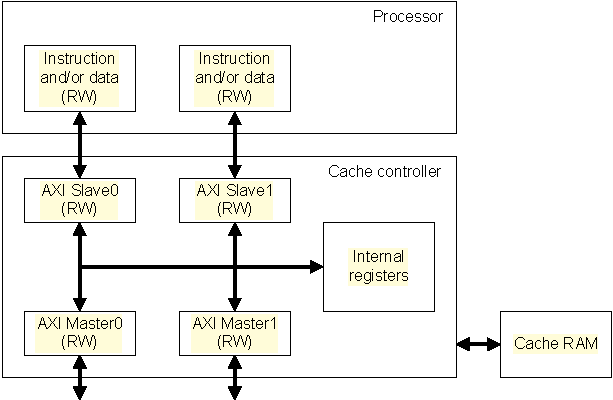
\includegraphics[width=0.9\linewidth]{example_cache_controller_interfaced_to_an_ARM_processor}
            \caption{Exemple de contrôleur de cache interfacé avec un processeur ARM \cite{manuel:coreLink_level_2_cache_controller_L2C_310}}
            \label{fig:example_cache_controller_interfaced_to_an_ARM_processor}
        \end{figure}

        \subsubsection{Impact sur les interférences}

            %\ijulien{Le cache de deuxième niveau est par défaut partagé entre les quatre cœurs du processeur peut être à l'origine de deux types d'interférences. Des \emph{interférences spatiales} lorsque les blocs de données chargés par un processeur sont évincées hors du cache par les pages utilisées par un autre cœur et des \emph{interférences temporelles} lorsque le cache reçoit un nombre de requêtes supérieur à celui qu'il peut gérer en parallèle, le premier type d'interférence pouvant être éliminé en utilisant le mécanisme matériel de verrouillage.}

            Le cache de deuxième niveau étant partagé entre les quatre cœurs du processeur, il est un canal pour deux types d'interférences.

            Tout d'abord, les caches partagés sont un canal d'interférence spatiale.
            Une application ordonnancée sur un cœur peut en effet évincer à son profit les données d'un applicatif ordonnancé sur un autre cœur.
            Il s'agit d'une des interférences le plus souvent mises en avant dans la littérature.
            Elles peuvent néanmoins être prévenues avec de la coloration de pages ou de manière équivalente avec la fonctionnalité de \emph{lockdown by master} fournie par notre carte.

            Le deuxième type d'interférences est temporel et à lieu au niveau du contrôleur PL310.
            En effet, ce dernier peut traiter un certain nombre de requête en parallèle.
            Lorsque sa capacité de traitement est dépassée, les requêtes sont traitées séquentiellement.
            Une politique d'arbitrage doit alors être appliquée sur les requêtes à traiter.
            Or, cette dernière n'est malheureusement pas documentée.

            % Si la présence de compteurs matériels au sein du cache L2, permet d'obtenir une mesure globale du trafic mémoire qui est généré par l'ensemble des cœurs, elle ne permet pas de différencier les différents cœurs consommateurs. Or, nous avons vu dans la section \ref{processeur:impacts_sur_nos_travaux} que les compteurs locaux à chaque cœur ne permettaient pas de mesurer la consommation effectuée dans les niveaux partagés de la hiérarchie mémoire. La mise en place d'une solution de régulation similaire à celle utilisée par MemGuard décrite précédemment dans la partie \ref{subsubsection:memguard} est donc impossible sur notre plate-forme.

    \subsection{Contrôleur mémoire}
    \label{subsection:controleur_memoire}

        %\itodo{Figure supprimer les bus inutilisés}

        \begin{figure}[!ht]
            \centering
            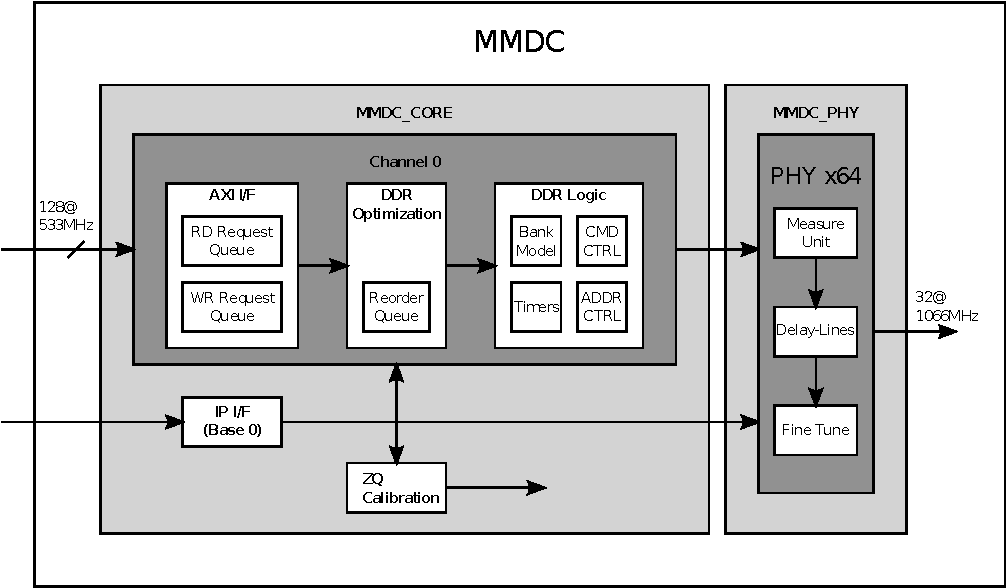
\includegraphics[width=\linewidth]{mmdc_block_diagram_2}
            \caption{Diagramme de bloc du contrôleur MMDC  \cite{manuel:i_MX_6Dual_6Quad_applications_processor_reference_manual}}
            \label{fig:mmdc_block_diagram_2}
        \end{figure}

        Le contrôleur mémoire MMDC (\emph{Multi Mode DDR Controller}) conçu par Freescale est chargé de gérer la mémoire DRAM de la plateforme matérielle. Il est constitué de deux composants, le \emph{cœur}, connecté à l'interconnecte NIC-301 par un bus AXI, gère la génération et l'optimisation des \emph{commandes mémoire} tandis que la partie \emph{PHY}, connectée à 1 giga de mémoire de type DDR3 \cite{manuel:SABRE_lite_hardware_user_manual} par un seul canal, est responsable de la gestion des \emph{timings}.

        %The MMDC module is a DDR controller that can support several types of DDR memories and two channel x32 and x64 memory widths.
        %MMDC is a multi-mode DDR controller that supports DDR3/DDR3L x16/x32/x64 and LPDDR2 two channel x16/x32 memory types. MMDC is configurable, high performance, and optimized.

        %MMDC consists of a core (MMDC\_CORE) and PHY (MMDC\_PHY).
        %\begin{itemize}
        %    \item The core is responsible for communication with the system through an AXI interface, DDR command generation, DDR command optimizations, and a read/write data path.
        %    \item The PHY is responsible for the timing adjustment; it uses special calibration mechanisms to ensure data capture margin at a clock rate of up to 533 MHz.
        %\end{itemize}

        %The core is composed of two channels, but both channels are only active in LPDDR2 mode. If DDR3 mode is selected, channel1 is not activated and the MMDC communicates with the system through AXI port0.

        Le cœur du contrôleur contient deux tampons \emph{FIFO} utilisés pour stocker temporairement les requêtes d'accès mémoire émises par les consommateurs. Le premier tampon est capable de sauvegarder jusqu'à 8 requêtes d'accès en écriture tandis que le deuxième, qui dispose d'une capacité de 16 entrées, est utilisé pour sauvegarder les requêtes d'accès en lecture.
        %
        Un mécanisme d'arbitrage de type \emph{round-robin} est utilisé pour sélectionner les requêtes d'accès en lecture et en écriture qui sont en attente et les envoyer dans un tampon intermédiaire de réordonnancement.

        Un mécanisme d'arbitrage est utilisé pour élire une requête au sein du tampon de réordonnancement et l'envoyer vers l'étage \emph{DDR Logic}, qui le découpe en commandes mémoire transmises à la mémoire DDR à travers le composant PHY. Une fois que les accès à la mémoire sont finis, la requête élue est supprimée du tampon de réordonnancement.
        %
        Le contrôleur mémoire met en œuvre une politique de gestion des \emph{row-buffer} de type \emph{open-row} que nous avons précédemment décrite en section \ref{subsection:controleur_memoire}.
        %
        %\optionnel{Le décodage d'adresse utilisé par le contrôleur mémoire est configurable. Il est notamment possible de choisir la politique de placement des données au sein des bancs mémoires. La politique de rafraîchissement du contrôleur mémoire est également configurable.}
        %
        Le décodage d'adresses utilise une politique de \emph{bank interleaving} dans laquelle les lignes consécutives en mémoire sont placées dans des bancs consécutifs.
        
        Afin d'optimiser l'utilisation du bus DDR, les requêtes d'accès sont réordonnancées dans le tampon de réordonnancement.
        Les requêtes présentes dans le tampon se voient attribuer un score afin de déterminer leur priorité, la requête avec le score le plus élevé est sélectionnée pour être envoyée vers le composant \emph{DDR logic}.
        Le score final est calculé en additionnant quatre facteurs différents et en tronquant les quatre bits de poids faibles:
        \begin{enumerate}
            \item \emph{Dynamic jump score} Ce score est incrémenté à chaque fois qu'une requête n'est pas sélectionnée.
            Ce score a une valeur maximale, égale à 15 sur notre cible.
            Lorsque cette valeur est atteinte, un mécanisme anti-famine est activé.
            
            \item \emph{Page hit score} Il s'agit d'un score statique attribué lorsque la ligne de destination de la requête est chargée dans un row buffer.
            Sur notre cible, ce score est égal à 4.
            
            \item \emph{Access score} Il s'agit d'un score statique attribué lorsque le type de l'accès (lecture ou écriture) est le même que celui de la requête sélectionnée précédemment.
            Sur notre cible, ce score est égal 2.

            \item \emph{QoS score} Il s'agit ici d'un score attribué dynamiquement par le matériel. Il est encodé sur 4 bits et ne peut donc pas dépasser 15. Mis à part cela, son mode de calcul n'est pas connu. Lorsque le mode temps réel du contrôleur mémoire est activé, toutes les requêtes avec un score QoS maximal deviennent prioritaires sur les autres requêtes.
        \end{enumerate}

        \begin{figure}[!h]
            \centering
            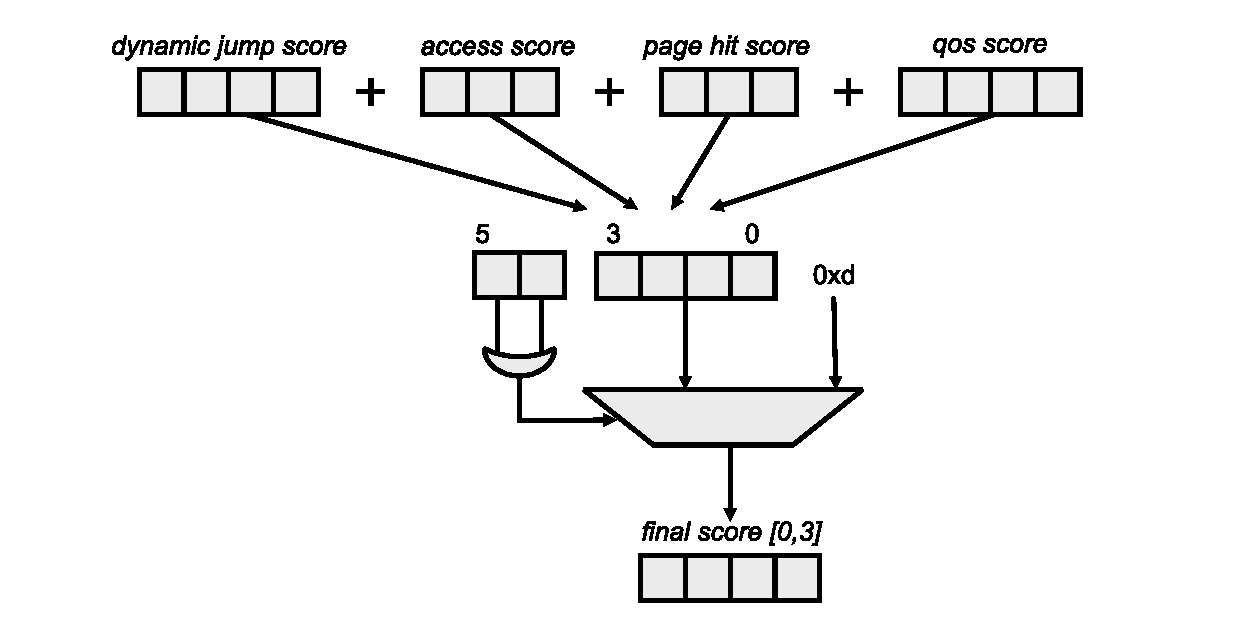
\includegraphics[width=0.75\linewidth]{mmdc-arbitration-score}
            \caption{\label{fig:mmdc_score}Calcul de la priorité lors du réordonnancement des accès DRAM}
        \end{figure}

        Lorsque le \emph{dynamic jump score} d'un accès atteint la valeur maximale, un mécanisme anti-famine est activé: un second compteur est incrémenté, jusqu'à atteindre une valeur maximale (fixée à 15 sur notre plateforme). 
        Lorsque le compteur associé à une requête atteint une valeur maximale, cette requête prend la priorité sur toutes les autres.

        Pour augmenter les performances de la mémoire, un mécanisme désactivable de prédiction permet de prédire, en parallèle du mécanisme d'arbitrage, la puce, le banc mémoire et la ligne qui vont être utilisée afin de préparer en avance la gestion des futurs accès. Selon la documentation~\cite{mmdc_dbi}, la prédiction se fait en utilisant notamment en considérant les accès au niveau du processeur, et du tampon de réordonnancement.

        Le contrôleur mémoire dispose d'un dispositif de profilage permettant de récupérer des statistiques sur l'utilisation de la mémoire (nombre d'accès effectués en lecture/écriture, trafic mémoire généré en lecture/écriture) et sur l'occupation du contrôleur mémoire (Nombre de cycles où le contrôleur est occupé). Un mécanisme de filtrage utilisant l'identifiant des bus AXI peut être mis en place pour éviter de comptabiliser le trafic mémoire généré par certains composants matériels (GPU, Ethernet, ....).

        \subsubsection{Impacts sur nos travaux}

            %\ijulien{
            %Le contrôleur mémoire va collecter l'ensemble des requêtes émis par les consommateurs pour les traduire, séquentiellement, en commandes mémoire. De multiples sources d'interférences sont présentes au sein de ce composant matériel.

            %Tout d'abord le nombre de requêtes pouvant être mises en attente au sein du contrôleur est borné, des requêtes devant être émises lorsque les tampons sont pleins doivent être retardée.

            %Ensuite, le contrôleur met en œuvre un algorithme sophistiqué qui à pour objectif d'augmenter le débit mémoire total de la plate-forme matérielle sans accorder une importance particulière aux performances temps réel de la machine. Les requêtes mémoires peuvent donc être réordonnancée, un processus effectuant une suite de commandes d'un même type (lecture ou écriture) vers une même \emph{row-buffer} se voyant priorisé par rapport à des processus effectuant un mixte de lecture et d'écritures.

            %L'utilisation d'une politique de \emph{bank interleaving} permet légalement d'accroître les performances au détriment de la prédictibilité, les données accédées par un processus se voyant réparties sur plusieurs bancs mémoire utilisés également par d'autres consommateurs.

            %Si la présence d'un mode temps réel au sein du contrôleur mémoire est prometteur puisqu'il permet de rajouter de la prédictibilité au détriment des performances, il ne peut être utilisé à la granularité d'un cœur, ce qui ne correspond pas à nos besoins.}

            %\itodo{Problème dans la partie d'avant je ne dis pas que le tag QoS est pas applicable}

            De multiples sources d'interférences sont présentes au sein du contrôleur mémoire qui va collecter l'ensemble des requêtes émises par les consommateurs pour les traduire, séquentiellement, en commandes mémoire.

            Tout d'abord, le nombre de requêtes pouvant être mises en attente au sein du contrôleur est borné par la taille des tampons de stockage des requêtes. Un consommateur qui émet un grand nombre de requêtes mémoires peut donc remplir les tampons du contrôleur retardant ainsi le traitement des requêtes des autres demandeurs.

            Une autre source d'interférences réside dans le réordonnancement des requêtes d'accès.
            En effet, le contrôleur cherche à maximiser les performances globales de la machine tout en évitant les conflits entre requêtes.
            Pour y arriver, le contrôleur mémoire réordonnance les requêtes de telle sorte à maximiser le débit mémoire total de la plateforme matérielle sans accorder une importance particulière aux performances temps réel de la machine. Un processus effectuant une suite de commandes de même type (lecture ou écriture) vers un même \emph{row-buffer} se voyant priorisé par rapport à des processus effectuant une combinaison de lectures et d'écritures.
            %
            Par conséquent, un programme qui effectue des accès favorisant une bonne bande passante peut devenir prioritaire et retarder les accès effectués par un autre programme exécuté en parallèle.

            L'utilisation d'une politique de \emph{bank interleaving} permet également d'accroître les performances au détriment de la prédictibilité, les données accédées par un processus se voyant réparties sur plusieurs bancs mémoire utilisés également par d'autres consommateurs.

            Enfin, l'utilisation d'une politique de gestion des pages de type \emph{open-row}, telle qu'utilisée par le contrôleur MMDC, introduit des dépendances temporelles entre les commandes mémoire. En effet, les temps d'accès à une cellule mémoire sont conditionnés par l'état du banc mémoire qui dépend des commandes exécutées précédemment. Des commandes mémoire émises par un cœur critique peuvent donc entrer en conflit avec celles émises par un cœur non critique générant ainsi des ralentissements.

        % \paragraph{Functional Description}
        %
        %     \subparagraph{Write data flow}
        %
        %         \begin{enumerate}
        %             \item Write requests are received into an 8 entries request FIFO. Access is received only when there are at least two available entries. Each entry holds all of the AXI attributes.
        %             \begin{itemize}
        %                 \item If the burst length is greater than 8, the access splits into two accesses: one with burst length 8 and the other with the remainder.
        %                 \item The access can be performed as soon as the entire data phase of the associated write request is completed (all data beats were received).
        %             \end{itemize}
        %             \item  A simple round-robin arbitration between the pending read and write accesses is performed, and the pointer to this stage's winner access is sent to the re-ordering buffer.
        %             \item The reordering mechanism is activated to find the winner access, which is the access that best utilizes the DDR bus, based on its dynamic score. For further information see Dynamic scoring mode (Arbitration Winning Conditions).
        %             \item  The winner write access at the previous stage is received and is held for dispatch to the DDR logic.
        %             \item  When the DDR command control unit is ready to accept the write request, it issues (if needed) a precharge/active command to the DDR device according to the status of the bank model and the parameters of the timers.
        %             \item  The DDR logic drives the associated data to the DDR device through the DDR PHY.
        %         \end{enumerate}
        %
        %     \subparagraph{Read data flow}
        %
        %         \begin{enumerate}
        %             \item Read requests are received into a 16 entry request FIFO in MMDC if there are at least two available entries. Each entry holds all of the AXI attributes. NOTE If the burst length is greater than 8, the access splits into 2 accesses (one with burst length 8 and the other with the remainder).
        %             \item A simple round-robin arbitration between the pending read and write accesses is performed and the pointer to this phase's winner access is sent to the re-ordering buffer.
        %             \item The reordering mechanism is activated to find the winner access, which is the access that best utilizes the DDR bus, based on its dynamic score. For further information see Dynamic scoring mode (Arbitration Winning Conditions).
        %             \item The winner read access at the previous stage is sampled and is held for dispatch to the DDR logic. This read access will be dispatched when there is at least one free slot in the read data buffer to store the data.
        %             \item When the DDR command control unit is ready to accept the read request, it issues (if needed) a precharge/active command to the DDR device according to the status of the bank model and the parameters of the timers.
        %             \item The MMDC PHY samples the read data, and the DDR logic transfers the data to the associated slot in the read data buffer.
        %             \item MMDC transfers the data back to the master.
        %         \end{enumerate}

        % \subparagraph{Address decoding}
        %
        %     The following registers in the MMDC define the DDR address space:
        %     \begin{itemize}
        %         \item MDMISC[DDR\_4\_BANK]—Defines either 4 or 8 banks in the DDR device
        %         \item MDCTL[DSIZ]—Defines the DDR data bus width of x16, x32 or x64
        %         \item MDMISC[BI]—Defines whether bank interleaving is on or off
        %         \item MDCTL[COL]—Defines the column size of the DDR device
        %         \item MDCTL[ROW]—Defines the row size of the DDR device
        %     \end{itemize}

        % \subparagraph{Chip select settings}
        %
        %     MMDC drives the incoming access to either CS0 or CS1 by comparing the 7 most significant address bits (ARADDR[31:25]/AWADDR[31:25]) with MDASP[CS0\_END].

        % \subparagraph{Refresh Scheme}
        %
        %     The periodic auto refresh can be triggered by the following clocks:
        %     \begin{itemize}
        %         \item 32KHz clock
        %         \item 64KHz clock
        %         \item MMDC operating clock
        %     \end{itemize}

        % \subparagraph{Burst Length options towards DDR}
        %
        % The MMDC supports two kinds of burst lengths which can be configured through MDCTL[BL] as follows: In DDR3 mode, only burst length 8 can be used.
        %
        % In DDR3 mode read/write accesses to the DDR are always 8 words (x16, x32, x64) and aligned in according to JEDEC standards.


        % \paragraph{Performance}

        % \subparagraph{Arbitration General}
        %
        %     The following specifies arbitration and reordering flow in MMDC towards the DDR.
        %     \begin{itemize}
        %         \item AXI read and write accesses are sampled in the associated queue.
        %         \item Read/write arbitration is handled to select the winning access.
        %         \item Winning access is sampled in the reordering queue
        %         \item Reordering mechanism is handled between valid requests that reside in the reordering queue to select the access that will be dispatched to the DDR.
        %         \begin{itemize}
        %             \item The reordering is held in order to optimize the accesses and to maximize the utilization of the DDR bus
        %             \item As soon as the reordered access is completed (indicated by end of response or data phase) then it is erased from the associated queue and the MMDC is ready to receive the next available access from the master
        %         \end{itemize}
        %     \end{itemize}
        %
        %     In general, the reordering/arbitration mechanism is based on dynamic priority mechanism, which compares dynamic priorities between valid entries in the reordering queue and issues the entry with highest dynamic priority towards the DDR Logic.
        %
        %     The selection of the winning access is based on two modes, which can be activated together, as following:
        %     \begin{itemize}
        %         \item Real time channel mode:
        %         \item Accesses with QoS='f' (i.e. awqos[3:0]/arqos[3:0] = "f") will bypass all other requests towards the DDR
        %         \item Dynamic scoring mode:
        %         \item The arbitration mechanism is based on dynamic priority. Relevant for the accesses with QoS smaller than 'f' or when real time channel mode is disabled.
        %     \end{itemize}
        %
        %     Due to re-ordering and optimization mechanism (per different AXI ID), the transactions towards the DDR may be driven in a different ID order they were received by the AXI master. In similar way, the write response, read response or read data may be driven to the AXI master in a different ID order.
        %
        % \subparagraph{Real time channel mode}
        %
        %     When real time mode is enabled (i.e MAARCR[ARCR\_RCH\_EN] = "1") , all requests with QoS='f' (i.e. awqos[3:0]/aqqos[3:0] = "f") will bypass all other pending accesses towards the DDR. This mode is enabled by default.
        %
        % \subparagraph{Dynamic scoring mode (Arbitration Winning Conditions)}
        %
        %     The arbitration between pending accesses in the MMDC is handled according to a dynamic priority of each access.
        %
        %     The dynamic priority (may be also called score) is calculated according to a sum of some factors (final\_score[3:0]), where part of them may be updated dynamically. The following will specify each scoring factor:
        %
        %     \begin{itemize}
        %         \item MAARCR[ARCR\_PAG\_HIT] (Page hit score) - A static score which is taken into account in case the pending access has a page hit
        %         \item MAARCR[ARCR\_ACC\_HIT] (Access hit score) - A static score, which is taken into account in case the current access type (read/write) is the same as the access that has been dispatched to the DDR previously
        %         \item MAARCR[ARCR\_DYN\_JMP] (Dynamic jump score) - A dynamic score which is given to any pending access in case it was not chosen in the arbitration. The dynamic jump counter is limited by maximum value which is set in MAARCR[ARCR\_DYN\_MAX] .
        %         \item QoS score which is indicated through a sideband 4bits AXI signals (awqos[3:0]/aqqos[3:0]) and is driven by the AXI master per access
        %     \end{itemize}
        %
        %     Note: In order to prevent an overflow in the total sum of scores, a clipping is held and selects the maximum score value of 'f' once a total scores sum is greater than 'f'.
        %
        % \subparagraph{Guarding (aging) mechanism}
        %
        %     The guarding mechanism (may be also called aging) is used to prevent a starvation of accesses.
        %
        %     As soon as the dynamic jump score reaches its maximum value (MAARCR[ARCR\_DYN\_MAX] ) then each time a pending request was not chosen in the arbitration, the "guarding" counter is incremented by 1. When the "guarding" counter reaches its predefined value, set in MAARCR[ARCR\_GUARD], the associated request gets the highest priority and will be chosen in the next arbitration cycle towards the DDR unless a real time channel (i.e access with QoS ="f") is arrived.
        %
        %     Note: In case real time channel has arrived then the dynamic score of the non real time channels won't increment in order to prevent a case where the "guarding" counter of more than one access has reached its limit.

        % \subparagraph{Prediction mechanism}
        %
        %     When prediction mechanism is enabled (i.e by configuring MDMISC[MIF3\_MODE]) then the MMDC predicts the chip-select, bank address and row address that is going to be issued towards the DDR before the access is physically dispatched towards DDR device. That mechanism enables to prepare the DDR device with future accesses and improves the overall DDR performance.
        %
        %     This prediction mechanism operates in parallel to the reordering mechanism and may yield a prediction based on 3 levels of pending accesses:
        %     \begin{enumerate}
        %         \item Access in first stage of pipeline.
        %         \item Valid access on AXI bus either read channel or write channel.
        %         \item Valid access on special bus from arbit
        %     \end{enumerate}

%             \paragraph{MMDC Profiling}

        % The profiling mechanism provides the ability to calculate the DDR utilization together with read and write accesses statistics towards DDR per given period of time.
        %
        % MMDC supports the following profiling counters:
        % \begin{itemize}
        %     \item MADPSR0 (Total cycles count) - Indicates the total amount of cycles of the profiling period (up to 2^32 cycles)
        %     \item MADPSR1 (Busy cycles count) - Indicates the total busy cycles during the profiling period
        %     \item MADPSR2 (Total read accesses count) - Indicates the total read accesses towards MMDC during the profiling period
        %     \item MADPSR3 (Total write accesses count) - Indicates the total write accesses towards MMDC during the profiling period
        %     \item MADPSR4 (Total read bytes count) - Indicates total bytes that were read from MMDC during the profiling period
        %     \item MADPSR5 (Total write bytes count) - Indicates total bytes that were written to MMDC during the profiling period
        % \end{itemize}
        %
        % Read/Write statistics can be collected per specific AXI ID (16bits). The following fields in MADPCR1 register determines which AXI-ID or AXI-ID's to monitor:
        % \begin{itemize}
        %     \item PRF_AXI_ID defines which AXI IDs are taken for profiling. Default values is 16'h0.
        %     \item PRF_AXI_ID_MASK defines which bits from PRF_AXI_ID will be compared with AXI ID of read/write access. "1" means to monitor the associated bit and "0" means don't care. Default value is 16'h0000, meaning all IDs are monitored
        % \end{itemize}

        % Table 6-1. MMDC feature summary
        %
        % Supported standards • LV-DDR3, DDR3 x16, x32, x64 (includes SODIMM)
        %     • LPDDR2 2ch x32, in either split map or interleaving mode
        %     • LPDDR2 1ch x32
        %
        % DDR interface • x16, x32, x64 data bus width
        %     • Density of 256 Mbytes-8 Gbytes
        %     • Column size of 8-12 bits
        %     • Row size of 11-16 bits
        %     • 2 CS per channel, with a separate CS allocation for LPDDR2-DRAM)
        %     • Up to 4 Gbyte address space and configurable address space per CS. For LPDDR2 2ch x32 up to 2 Gbytes per channel
        %     • Interleaved accesses of LPDDR2-DRAM towards the same DDR channel. This is supported only when using the same clock frequency for LPDDR2-DRAM
        %     • Supports burst length of 8 (aligned) for DDR3 and burst lengths of 4 for LPDDR2
        %
        % DDR performance
        %     • DDR3 and LPDDR2 support up to 1066MT/s transfer rate
        %     • Supports Real-Time priority by means of QoS sideband priority signals from the chip to enable different priority levels in the re-ordering mechanism
        %     • Page hit/page miss optimizations
        %     • Consecutive read/write access optimizations
        %     • Supports deep read and write requests queues to enable bank prediction
        %     • Drives back the critical word in a read transaction as soon as it is received by the DDR device (doesn't wait until the whole data phase has been completed)
        %     • Can track open memory pages
        %     • Supports bank interleaving
        %     • Special optimization for non-aligned wrap accesses in burst length 8 AXI interface
        %     • AXI bus compliant with glueless interface to PL301 AXI network interconnect
        %     • Supports bus transfers of 8,16,32, 64 and 128 bits (single accesses and bursts)
        %
        % DDR calibration and delay-lines
        %     • All calibrations can be done automatically by hardware or manually by software
        %     • ZQ calibration for external DDR device (in DDR3 through the ZQ calibration command and in LPDDR2 through the MRW command).
        %     • Can be handled automatically for ZQ Short (periodically) and ZQ Long (at exit from self-refresh).
        %     • Can be handled manually at ZQ INIT.
        %
        % DDR general
        %     • Configurable timing parameters
        %     • Configurable refresh scheme
        %     • Supports dynamic voltage, frequency change and low power mode entry through hardware negotiation with the system (req/ack handshake)
        %     • Suppors automatic self-refresh and power down entry and exit
        %     • Supports fast and slow precharge power down in DDR3
        %     • Supports various ODT control schemes.
        %     • Assertion/Deassertion of ODT control per read or write accesses and for active or passive CS
        %     • Supports MRW and MRR commands for LPDDR2.
        %     • Software control for moving to derated timing parameters and derated refresh rate according to temperature variation.
        %     • Supports various debug and profiling modes

    % ===============================
    % ============ netys ============
    % ===============================
    %
    %\subsection{Hardware}
    %
    %    We focus on embedded systems, as used in the automotive domain, which has strong hardware cost requirements. Therefore, for our tests we use the SABRE Lite board \cite{MANUAL:IMX6_DQRM}, a low-cost development platform designed for multimedia applications on the Android and Linux operating systems. A variant of this platform that has been adapted for the automotive domain is used by a large number of automotive manufacturers and suppliers
    %
    %    The processor of the SABRE Lite is an i.MX 6, which is based on a 1.2 GHz quad-core Cortex A9 MPCore \cite{MANUAL:A9_MPCORE_TRM}. Each core has a separate Level 1 (L1) 32-kilobyte 4-way set-associative cache for instructions and data \cite{MANUAL:A9_TRM}. All CPUs are connected to a single 1-megabyte 16-way set-associative L2 cache \cite{MANUAL:L2C310_TRM} that can be partitioned into multiples of the way size. Finally, the Multi Mode DRAM Controller (MMDC) manages access to one gigabyte of DDR3 RAM that can be used by all the cores \cite{MANUAL:IMX6_DQRM}.
    %
    %    The SABRE Lite board provides various hardware performance counters. Each core provides six configurable counters to gather statistics about the operation of the processor (number of cycles) and the memory system (L1 cache hits/misses) \cite{MANUAL:ARMV7,MANUAL:A9_TRM}. The MMDC has a profiling mechanism that gathers statistics (read/write bytes/access)  about the global memory traffic on the platform.

    % ===============================
    % ============ ECRTS ============
    % ===============================
    %
    %\subsection{Architecture of the SABRE Lite}

    %    In this paper, we target embedded systems, as used in the automotive domain, which has strong hardware cost requirements. We choose the SABRE Lite multicore system \cite{MANUAL:IMX6_DQRM} (see Figure~\ref{fig:archiIMX6}) since it has already been adopted by some industry leaders as an experimental platform.

    %    The processor of the SABRE Lite is an i.MX 6, which is based on a 1.2 GHz quad-core Cortex A9 MPCore \cite{MANUAL:A9_MPCORE_TRM}. Each core has two 32-kilobyte 4-way set-associative L1 caches, one for data and the other for instructions. Each core is also connected to an external 1-megabyte 16-way set-associative L2 cache \cite{MANUAL:L2C310_TRM} that can be either shared by all the cores or partitioned in multiples of 1/16th of the cache size. The Multi Mode DRAM Controller (MMDC) manages access to one gigabyte of DDR3 RAM that can be used by all cores \cite{MANUAL:IMX6_DQRM}. Each core contains six configurable hardware counters to gather statistics on the operation of the processor (number of cycles, etc.) and the memory system (L1 accesses, L1 misses, etc.) \cite{MANUAL:ARMV7, MANUAL:A9_TRM}.  The MMDC contains hardware counters that measure global memory traffic (read/write bytes, read/write accesses, etc.)  on the platform \cite{MANUAL:IMX6_DQRM}, but no hardware counter is provided to identify the core that is the source of a L2 miss.

    %    On the SABRE Lite, when using DDR3 RAM, the MMDC is accessible through a single AXI channel.  This AXI channel has two dedicated request queues: a 16 entry queue for read requests and a 8 entry queue for write requests. Each request queue entry holds the information to access up to one cache line. A round-robin arbitration mechanism is used to send pending read and write requests into a final reordering buffer, before the request is sent to the RAM.  We will show in Figure \ref{microbench_delay_bandwidth} that this mechanism has a significant impact on the bandwidth that can be achieved when mixing read and write accesses.

        % \begin{figure}[!ht]
        %     \centering
        %     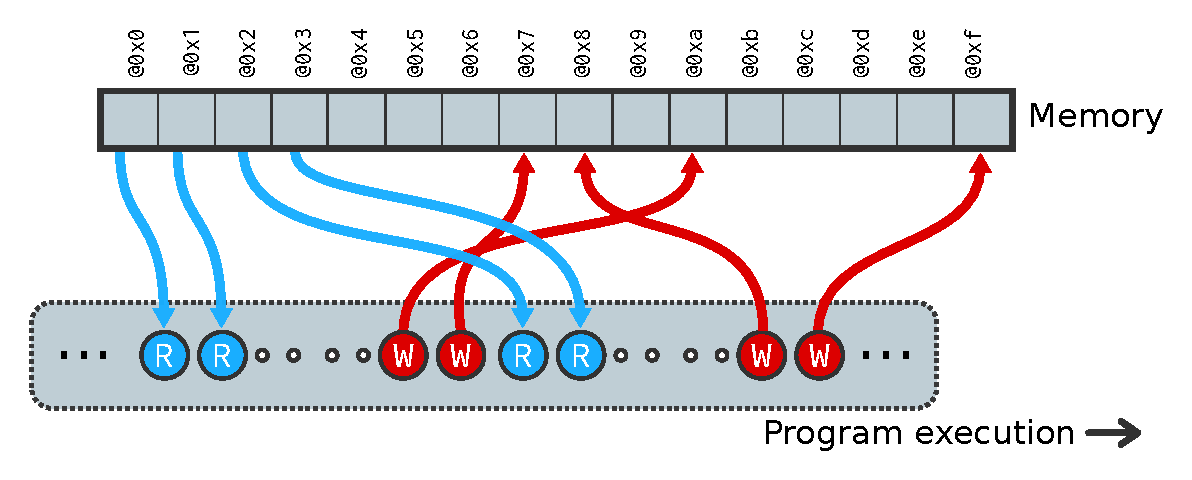
\includegraphics[scale=0.4]{memory}
        %     \caption{Architecture of the SABRE Lite board}
        %     \label{fig:archiIMX6}
        % \end{figure}

    %\subsection{Autre}
    %
    %    \itodo{Faut-il détailler les TLBs?}
    %    \ijulien{Oui mais pas le temps}
    \subsection{Récapitulatif}

Le tableau \ref{table:recapitulatif_hierarchie_memoire} contient, pour les multiples niveaux de la hiérarchie mémoire de notre carte, un récapitulatif des différentes caractéristiques matérielles qui sont partie prenante du problème de contention mémoire, à savoir, la taille et la politique de correspondance et de remplacement des différents composants.
        %
Dans une dernière colonne, nous avons aussi noté les métriques disponibles pour l’élaboration d’un nouveau mécanisme de contrôle.

\begin{table}[!h]
    \renewcommand{\arraystretch}{1.5}
    \resizebox{\linewidth}{!}{
    \begin{tabular}{l l l l l l}
        \toprule
        \multicolumn{2}{l}{\textbf{}} & \textbf{} & \textbf{} & \textbf{} & \textbf{Métriques}\\
        \multicolumn{2}{l}{\textbf{Composant}} & \textbf{Taille} & \textbf{Correspondance} & \textbf{Remplacement} & \textbf{Disponibles}\\
        \midrule
        \multirow{2}{*}{Cache L1} & Donnée & \multirow{2}{*}{32KiB} & 4 & PLRU ou PR & \multirow{2}{*}{PMU locale}\\
                                  & Instructions & & 4 & PR & \\
 
        \multicolumn{2}{l}{Cache L2} & 1MiB & 16 & PLRU ou PR & PMU globale \\

        \midrule
        \multicolumn{2}{l}{\textbf{}} & \textbf{} & \textbf{Nombre de bancs} & \textbf{} & \textbf{}\\
        \midrule
        \multicolumn{2}{l}{Mémoire principale} & 1GiB & 8 & N/A & PMU globale \\
        \bottomrule
        
    \end{tabular}
    }
    \caption{Récapitulatif des caractéristiques matérielles des différents niveaux de la hiérarchie mémoire.}
	\label{table:recapitulatif_hierarchie_memoire}
\end{table}


\section{Un modèle événementiel du trafic mémoire}

Pour étudier la sensibilité des programmes aux interférences mémoires, nous devons représenter l'interaction entre une application et le système mémoire.
Nous adopterons à cette fin un \emph{modèle événementiel} du trafic mémoire représentant le \emph{flux explicite de requête d'accès vers un système mémoire partagé} qui sont générées lors de l'exécution d'un programme.

L'exécution d'un programme est représentée par sa \emph{trace}, c'est à dire par la suite d'instructions qui ont été exécutées.
Une trace correspond au parcours d'un chemin dans le graphe de flots de contrôle.
Nous supposerons toujours la terminaison du programme, et donc que le nombre d'instructions dans une trace est fini.
Nous noterons celui-ci $N_{inst}$.

L'exécution d'une instruction entraîne une interaction avec le matériel, qui peut impliquer des éléments partagés du système mémoire.
Afin de ne pas modéliser le matériel en détail, et dans un souci de généricité, ces éléments sont regroupés dans une \emph{boite noire} représentant la mémoire partagée dans son ensemble.
Lorsqu’ une instruction interagit avec un composant appartenant à cette boite noire, une \emph{requête d'accès} est émise vers celle-ci.
Une requête d'accès peut être émise dans deux cas précis:
\begin{itemize}
	\item Lors d'une instruction d'accès à la mémoire.
	\item Lors du chargement d'une instruction.
\end{itemize}
Nous pouvons ainsi associer à toute trace d'exécution une suite de requêtes d'accès émises.
Cette suite est également finie, et nous notons son nombre d'éléments $N_{access}$.
Une requête mémoire est caractérisée par un \emph{sens}, une instruction de source et une adresse de destination.

Ce modèle représente le trafic généré \emph{explicitement} par l'application.
Sur un processeur moderne, le trafic généré peut être différent.
Il y a deux raisons à cela.
D'une part, les instructions peuvent être exécutées dans le désordre.
D'autre part, les mécanismes spéculatifs (prédiction de branchements, préchargements de données) peuvent également entraîner des accès qui ne sont pas représentés par le modèle.
Ce trafic \emph{implicite} varie fortement en fonction du matériel considéré.
Pour le prendre en compte, il faudrait pouvoir modéliser finement ce dernier, ce qui serait incompatible avec une vision boite noire de celui-ci.

La trace considérée correspond à la suite d'instruction obtenue en parcourant le graphe de flot de contrôle du programme.
Sur un processeur moderne, ces instructions peuvent être exécutées dans un ordre différent.
De plus, les mécanismes de spéculation (prédiction de branchements, préchargement de données) peuvent causer des accès supplémentaires qui ne sont pas capturés.
C'est une limitation de cette représentation.

Nous aurons par la suite souvent recours à une représentation graphique de l'activité mémoire.
La trace d'exécution y est représentée par une suite de points colorés.
Les instructions ne déclenchant pas d'accès vers la mémoire y sont représentées par des petits points gris, tandis que les déclenchant des accès sont représentés par de gros points colorés (bleu pour les requêtes en lecture et rouge pour les requêtes en écriture).
La flèche indique le sens d'exécution~\footnote{En cas d'omission de cette flèche, on considérera le sens de lecture habituel. C'est à dire gauche à droite et de haut en bas.}.
Cette représentation nous donne de premières indications sur les variations de comportements d'accès à la mémoire.
Cette représentation de la trace permet d'identifier aisément plusieurs caractéristiques du comportement d'accès à la mémoire.
La proportion d'accès à la mémoire par rapport au nombre total d'instructions exécutées indique l'intensité de l'utilisation de la mémoire.
La représentation des types d'accès permet de caractériser la proportion de lectures et d'écritures, mais aussi de leur entrelacement.

\begin{center}
	
\includegraphics[width=0.8\linewidth]{graphics/figures/template-profils-evenementiels-trace.pdf}
\end{center}

Nous pouvons également représenter l'interaction avec la mémoire.
Cette dernière est représentée par un tableau de case mémoire.
Chaque case est identifiée par une adresse.
Comme pour la trace d'exécution une flèche indique dans quelle direction évoluent les adresses\footnote{La remarque faite précédemment pour le sens de lecture des traces d'exécutions en cas d'omission de la flèche s'applique également pour la mémoire.}.

\begin{center}
	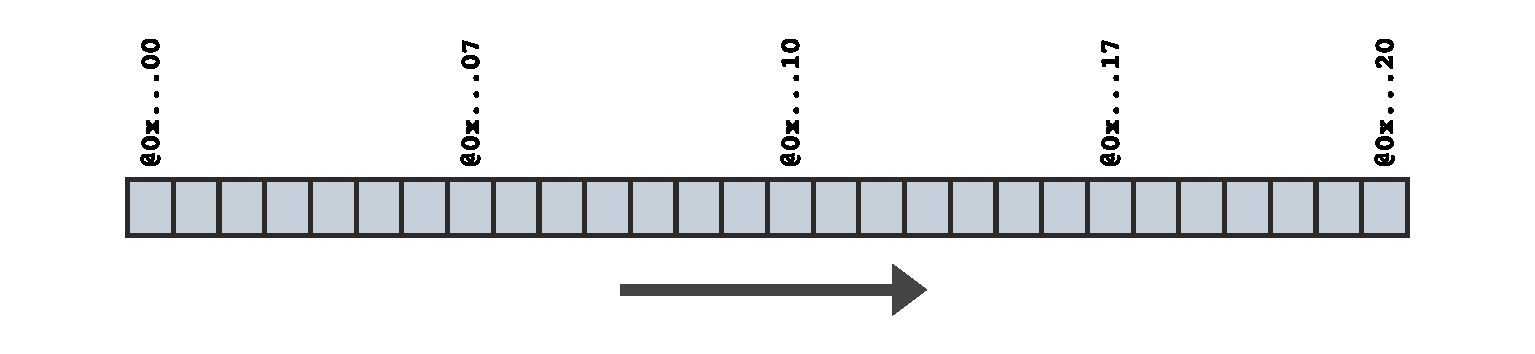
\includegraphics[width=0.8\linewidth]{graphics/figures/template-profils-evenementiels-memoire.pdf}
\end{center}

Enfin, l'interaction entre la trace d'exécution et la mémoire est représentée par des flèches.
Ces flèches, et en particulier leur entremêlement, permettent de juger du type de séquence d'accès effectués.

\begin{center}
	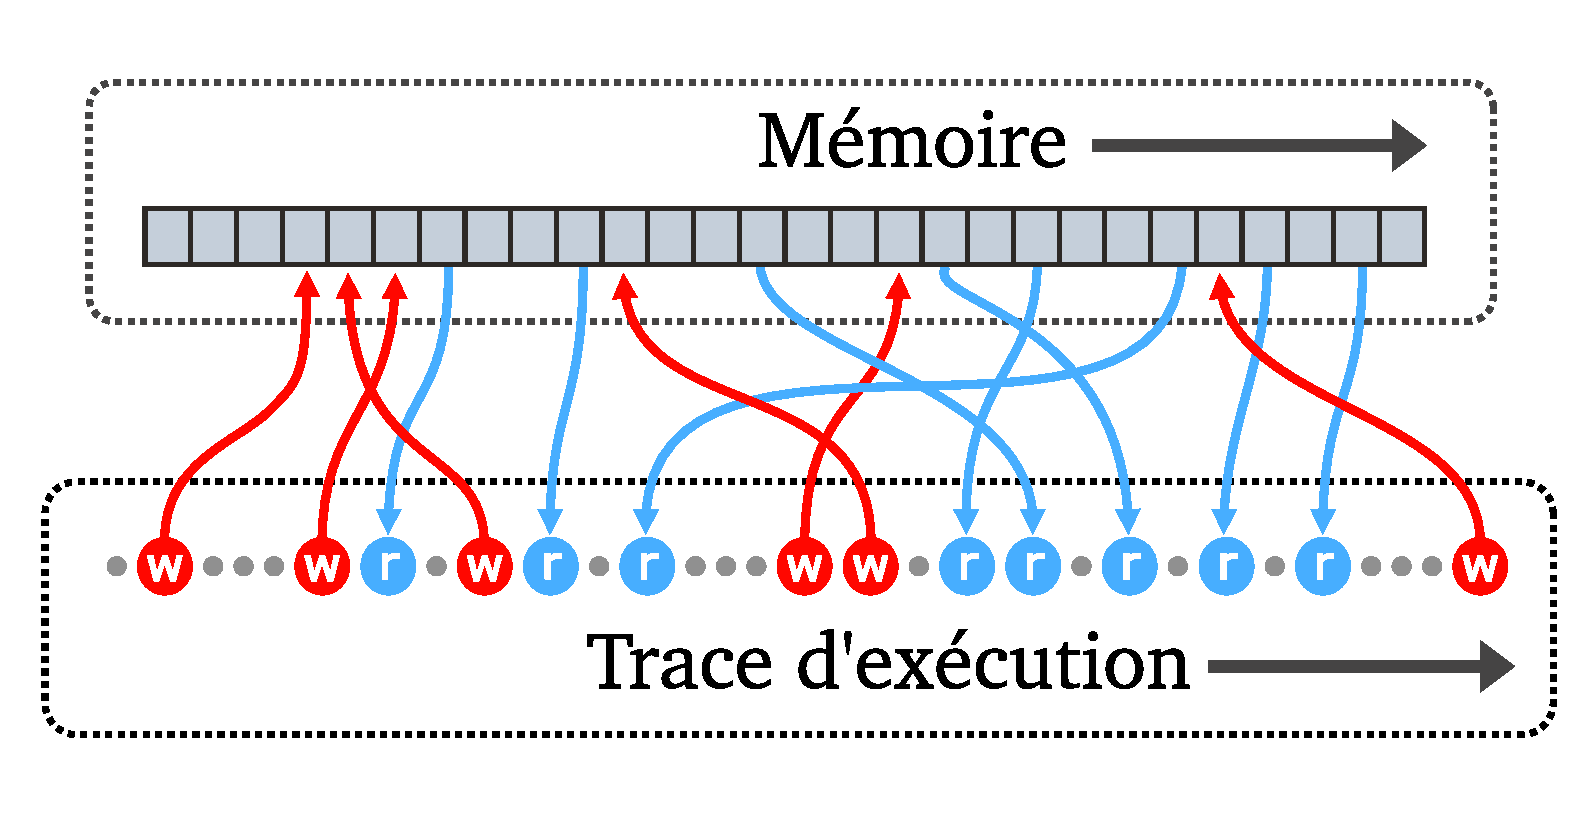
\includegraphics[width=0.8\linewidth]{graphics/figures/template-profils-evenementiels-all.pdf}
\end{center}

\section{Microbenchmarks}

Afin d'évaluer l'impact des interférences sur une cible matérielle donnée, nous souhaitons pouvoir reproduire une multitude de cas de consommation mémoire différents.
Si des microbenchmarks destinés à l'étude du système mémoire existent, par exemple \textsc{STREAM}~\cite{McCalpin1995}, ils ne sont pas adaptés à nos besoins, car destinés à l'évaluation des limites de performances des systèmes mémoires.
\textsc{STREAM}, par exemple, génère le trafic le plus intense possible en ne suivant qu'un seul type de séquence d'accès.

Nos microbenchmarks diffèrent des solutions existantes, car ils sont conçus dans l'objectif d'offrir la possibilité de générer des comportements d'accès variés, aussi bien en nature qu'en intensité.
À cet effet, nous avons conçu un algorithme générique pour varier les comportements mémoires, dont le pseudocode est donné par l'algorithme~\ref{alg:microbench}.
Cet algorithme consiste en la répétition d'une séquence d'accès vers une structure de données en mémoire.
Cette séquence consiste en trois étapes:
\begin{enumerate}
	\item Une \emph{boucle de lecture} durant laquelle des données sont lues depuis la mémoire et agrégées dans une variable.
	\item Une \emph{boucle de calcul}, dans laquelle la valeur agrégée dans la boucle d'écriture est transformée à l'aide d'opérations arithmétiques simples.
	Le but de cette boucle est d'inhiber le trafic généré par le microbenchmark en faisant des opérations ne mettant en jeu que des ressources locales à un cœur.
	\item Une \emph{boucle d'écriture} où la valeur produite par la boucle de calcul est écrite en mémoire.
\end{enumerate}

% \begin{figure}[!h]
% 	\centering
% 	\begin{tabular}{c c}
% 	\begin{subfigure}{0.25\linewidth}
% 		%\centering
% 		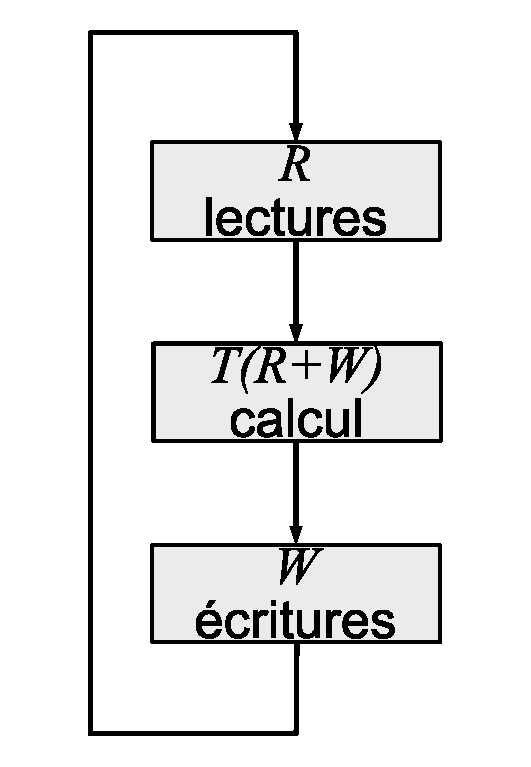
\includegraphics[width=\linewidth]{graphics/figures/algo-sequences-rcw.pdf}
% 		\caption{\label{fig:sequences_rcw}RCW}
% 	\end{subfigure} &
	
% 	\begin{subfigure}{0.25\linewidth}
% 		%\centering
% 		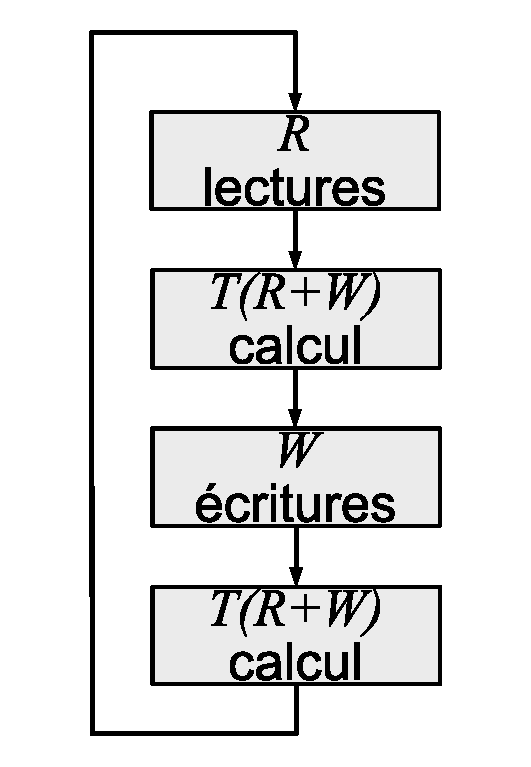
\includegraphics[width=\linewidth]{graphics/figures/algo-sequences-rcwc.pdf}
% 		\caption{\label{fig:sequences_rcwc}RCWC}
% 	\end{subfigure} \\
% 	\end{tabular}
% \end{figure}

\begin{algorithm}
\begin{algorithmic}

\Function{AccessSequence}{$(R, W, C, P_R, P_W)$}
  \For{$i \gets \text{1 to $N$}$}
  \Comment{La séquence est répétée $N$ fois}
	  \For{$j \gets \text{1 to $R$}$}
	  \Comment{Boucle de lecture}
	  \State{$v \gets P_R.read(R, pos, v)$}
	  \State{$pos \gets pos + R$}

	  \EndFor
	  
	  \For{$j \gets \text{1 to $C$}$}
	  \Comment{Boucle de calcul}
	    \State{$v \gets local\_computation(v)$}
	  \EndFor
	  
	  \For{$j \gets \text{1 to $W$}$}
	  \Comment{Boucle d'écriture}
	  	\State{$P_W.write(W, pos, v)$}
	  	\State{$pos \gets pos + W$}
	  \EndFor
  \EndFor
\EndFunction

\end{algorithmic}
\caption{\label{alg:microbench} Microbenchmark}
\end{algorithm}

Le comportement des trois boucles composants une séquence d'accès est configurable.
Ainsi, les paramètres $R$, $W$ et $C$ donne respectivement le nombre d'itérations des boucles de lectures, d'écritures et de calcul.

Le paramètre $C$ est directement lié à l'intensité du trafic généré par le microbenchmark, c'est-à-dire la proportion d'instructions générant des accès à la mémoire parmi toutes les instructions exécutées.
Cependant, l'effet de $C$ dépends directement des paramètres $R$ et $W$, car ceux-ci définissent le nombre d'accès à la mémoire effectuée lors d'une séquence d'accès.
C'est pourquoi nous utiliserons plutôt le nombre d'itérations de boucle de calcul pour désigner l'intensité supposée du trafic généré.

\begin{equation}
	F = \frac{C}{R+W}
	\label{eq:throttle_rate}
\end{equation}

Les paramètres $R$ et $W$ influent à la fois sur la proportion d'accès en lecture et en écriture du trafic généré, mais aussi sur l'entrelacement de ces accès et la longueur des rafales d'accès successifs vers la mémoire.
Ceci est illustré par le tableau~\ref{table:effet_parametres_sequence_acces} illustrant l'effet des paramètres $R$ et $W$, pour une valeur de $F$ et un nombre égal de lectures et d'écritures.
Ce tableau montre qu'un grand nombre total d'accès ($R+W$) implique à la fois un plus grand nombre d'accès successifs vers la mémoire, mais un plus faible entrelacement des lectures et des écritures.
Nous avons pu voir, dans la section~\ref{section:plateforme_materielle} que ces aspects sont pris en compte par la politique d'ordonnancement du contrôleur mémoire de notre plateforme matérielle.
Notre microbenchmark permet donc de générer des trafics mémoires de même intensité et de mêmes ratios lectures/écritures qui sont néanmoins significativement différents.

% \begin{figure}
% 	\begin{tabular}{c c}
% 	RCW & RCWC \\
% 	\begin{subfigure}[t]{0.5\linewidth}
% 		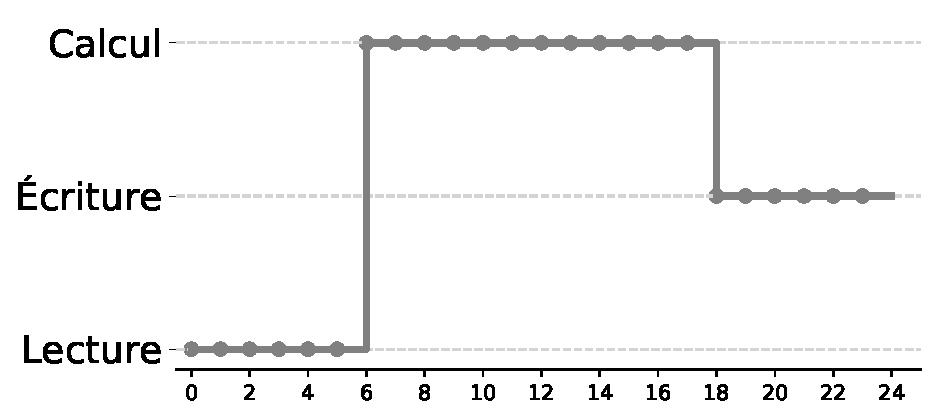
\includegraphics[width=\hsize]{graphics/figures/microbenchmark_tmp_rcw_6_6_12.pdf}
% 		\caption{$R=6$ $W=6$ $C=12$}
% 	\end{subfigure} & 
% 	\begin{subfigure}[t]{0.5\linewidth}
% 		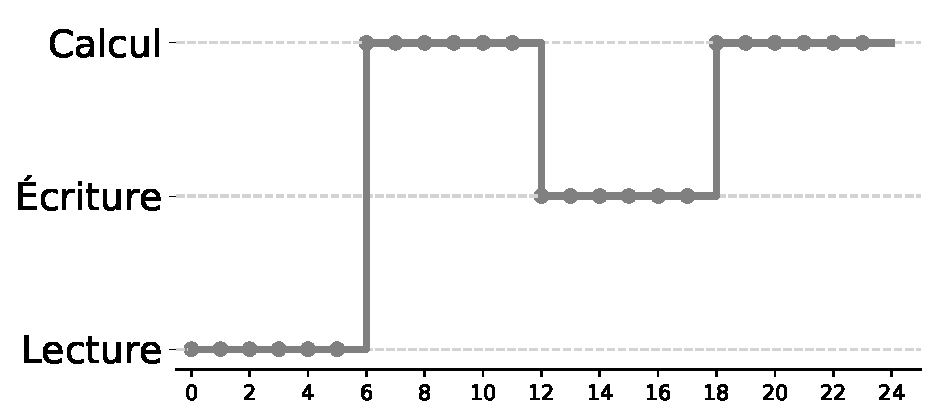
\includegraphics[width=\linewidth]{graphics/figures/microbenchmark_tmp_rcwc_6_6_12.pdf}
% 		\caption{$R=6$ $W=6$ $C=6$}
% 	\end{subfigure} \\
% 	\begin{subfigure}[t]{0.5\linewidth}
% 		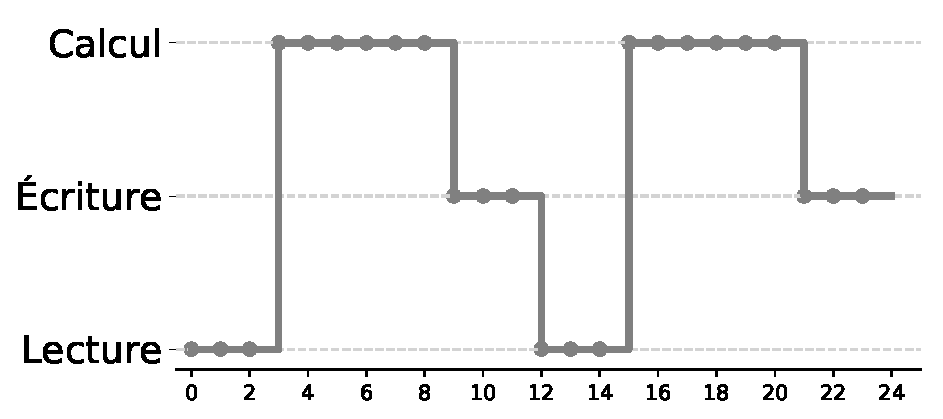
\includegraphics[width=\hsize]{graphics/figures/microbenchmark_tmp_rcw_3_3_6.pdf}
% 		\caption{$R=3$ $W=3$ $C=6$}
% 	\end{subfigure} & 
% 	\begin{subfigure}[t]{0.5\linewidth}
% 		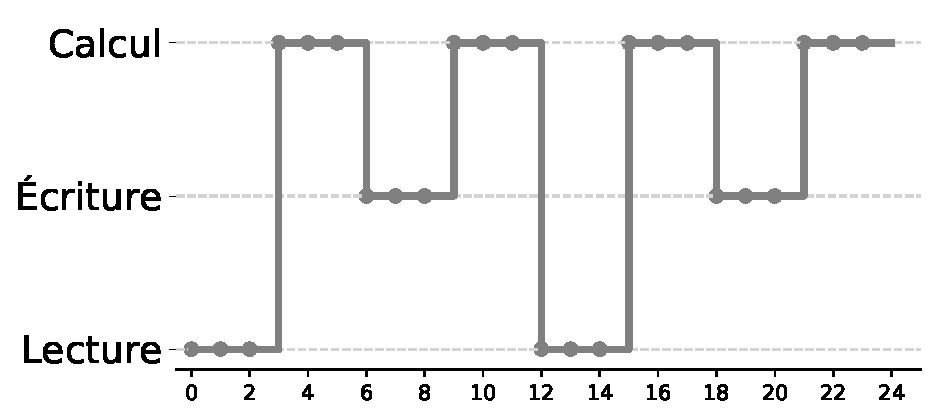
\includegraphics[width=\hsize]{graphics/figures/microbenchmark_tmp_rcwc_3_3_6.pdf}
% 		\caption{$R=3$ $W=3$ $C=3$}
% 	\end{subfigure} \\
	
% 	\begin{subfigure}[t]{0.5\linewidth}
% 		\includegraphics[width=\hsize]{graphics/figures/microbenchmark_tmp_rcw_1_1_2.pdf}
% 		\caption{$R=1$ $W=1$ $C=2$}
% 	\end{subfigure} &
	
% 	\begin{subfigure}[t]{0.5\linewidth}
% 		\includegraphics[width=\hsize]{graphics/figures/microbenchmark_tmp_rcwc_1_1_2.pdf}
% 		\caption{$R=1$ $W=1$ $C=1$}
% 	\end{subfigure} \\
% 	\end{tabular}
% 	\caption{\label{fig:microbenchmarks_params_effet_temporelle}}
% \end{figure}


\begin{table}[h!]
	\centering
	\caption{\label{table:effet_parametres_sequence_acces} Effet des paramètres $R$ et $W$ sur le trafic généré}
	\begin{tabular}{c c c c c r}
		$R$ & $W$ & $F$ & $C$& \\
		\midrule
		 1 & 1 & 1 & 2 & \raisebox{-0.525\totalheight}{\includegraphics[width=0.65\linewidth]{graphics/figures/templates-microbenchmarks-rcw-1-1-2.pdf}}\\
		 3 & 3 & 1 & 6 & \raisebox{-0.525\totalheight}{\includegraphics[width=0.65\linewidth]{graphics/figures/templates-microbenchmarks-rcw-3-3-6.pdf}}\\
		 6 & 6 & 1 & 12 & \raisebox{-0.525\totalheight}{\includegraphics[width=0.65\linewidth]{graphics/figures/templates-microbenchmarks-rcw-6-6-12.pdf}}\\
		 \bottomrule
	\end{tabular}
\end{table}

\subsection{Politique d'accès}

En plus de leur nombre d'itérations, le comportement des boucles de lectures et d'écritures peut être modifié par le biais de \emph{politique d'accès}, que nous désignons par les paramètres $P_R$ et $P_W$.
Nous avons défini et implanté sept politiques d'accès différentes, dont les caractéristiques sont résumées dans le tableau~\ref{table:recap_politiques d'accès}.
Ces politiques se distinguent notamment par le type de la structure de données accédées, ainsi que par la localité de la séquence des accès.

\begin{table}
	\centering
	\renewcommand{\arraystretch}{1.3}

	\begin{tabular}{r c c}
		\toprule
		\textbf{Politique} & \textbf{Structure de données} & \textbf{Type d'accès} \\
		\midrule
		\texttt{linear} & \multirow{2}{*}{tableau} & séquentiel \\
		\texttt{random} &  & aléatoire \\
		\midrule
		\texttt{linear-lookup} & \multirow{2}{*}{tableau de pointeurs} & séquentiel \\
		\texttt{shuffled-lookup} &  & séquentiel et aléatoire \\
		\midrule
		\texttt{linear-list} & \multirow{2}{*}{liste chaînée} & séquentiel \\
		\texttt{shuffled-list} &  & aléatoire \\
		\midrule
		\texttt{stream} & tableaux & parallèle et séquentiel \\
		\bottomrule
	\end{tabular}
	\caption{\label{table:recap_politiques d'accès}Récapitulatifs des différentes politiques d'accès}
\end{table}

\subsubsection{Structures de données}

Nous utilisons trois structures de données différentes:

\begin{description}
	\item[Tableau] Les données sont stockées dans un tableau. Ce sera le cas, quelle que soit la structure de donnée utilisée.
	Ici, les données sont accédées directement en utilisant l'indexation.
	\item[Tableau de pointeurs] Les données sont accédées en déférençant un pointeur. Les pointeurs sur les données sont stockés dans un tableau. Ce tableau est parcouru séquentiellement.
	\item[Liste chaînée] Tout comme pour les tableaux de pointeurs les données sont accédées en déferencant un pointeur. La différence est qu'ici ces pointeurs sont stockés dans une liste chaînée.
\end{description}

Le choix d'une structure de donnée à des implications sur les dépendances de données présentes dans les boucles de lectures et d'écritures, et plus particulièrement celles concernant les adresses des données accédées lors d'un tour de boucle.
Les dépendances de données ont pour effet de donner moins de liberté d'action au processeur pour le réordonnancement d'instructions.

Dans le cas d'un parcours de tableau(figure~\ref{fig:array-deps}), l'adresse est calculée directement, il n'y a donc pas de dépendances à proprement parler.
Il peut y avoir une dépendance entre les tours de boucles pour effectuer ce calcul, mais les valeurs en question étant généralement stockées dans des registres, celle-ci n'est pas significative.
L'utilisation d'un tableau de pointeurs (figure~\ref{fig:lookup-deps}), introduit une dépendance pour déterminer l'adresse de destination.
La conséquence est que le processeur ne peut pas réordonner les instructions au sein d'un même tour de boucle.
Par contre, vu que le tableau de pointeur est parcouru séquentiellement, les itérations peuvent l'être.
L'utilisation d'une liste chaînée (figure~\ref{fig:list-deps}) prévient ce degré de liberté en introduisant une dépendance de données entre les tours de boucles.

\begin{figure}
	\begin{tabular}{c c c}
		\begin{subfigure}{0.33 \linewidth}
			\includegraphics[width=\linewidth]{graphics/figures/array-dependencies.pdf}
			\caption{\label{fig:array-deps}Tableau}
		\end{subfigure}
		\begin{subfigure}{0.33 \linewidth}
			\includegraphics[width=\linewidth]{graphics/figures/lookup-dependencies.pdf}
			\caption{\label{fig:lookup-deps}Tableau de pointeurs}
		\end{subfigure}
		\begin{subfigure}{0.33 \linewidth}
			\includegraphics[width=\linewidth]{graphics/figures/list-dependencies.pdf}
			\caption{\label{fig:list-deps}Liste chaînée}
		\end{subfigure}
	\end{tabular}
	\caption{\label{fig:datastruct-deps}Dépendance de données intra et inter itérations pour les boucles d'accès mémoires en fonction de la structure de donnée utilisée.}
\end{figure}

\subsubsection{Politique d'accès}

Un deuxième aspect régi par la politique d'accès est la succession d'adresse accédée lors de la séquence.
Cela impacte notamment la localité spatiale du trafic émis par le microbenchmark.
Les différentes politiques que nous implantons peuvent générer des suites d'adresses pouvant être catégorisées en trois types:

\begin{itemize}
	\item \emph{Accès séquentiels (ou linéaires)} La différence entre deux adresses successives est constante.
	On appelle la différence entre deux adresses le \emph{pas (ou stride)}.
	Il s'agit d'un type d'accès très courant, qui est notamment généré lors l'on parcourt un tableau (figure~\ref{fig:seq-linear}).

	\item \emph{Accès aléatoires}. Il n'y a pas de relations claires dans l'enchaînement des adresses accédé.
	Il s'agit du comportement réciproque aux accès séquentiels.
	Nous utilisons ce type de séquence pour approximer les séquences d'accès les plus complexes (figure~\ref{fig:seq-linear}).
		
	\item \emph{Accès parallèle} Plusieurs séquences linéaires sont entrelacées.
	Ce type de séquence représente en particulier le parcours de plusieurs tableaux en parallèle (figure~\ref{fig:seq-linear}).
\end{itemize}

\begin{figure}[h!]
	\centering
	\begin{subfigure}{0.65\linewidth}
		\includegraphics[width=\linewidth]{graphics/figures/sequence-linear.pdf}
		\caption{\label{fig:seq-linear}Accès séquentiels}
	\end{subfigure}
	\begin{subfigure}{0.65\linewidth}
		\includegraphics[width=\linewidth]{graphics/figures/sequence-random.pdf}
		\caption{\label{fig:seq-random}Accès aléatoires}
	\end{subfigure}
	\begin{subfigure}{0.65\linewidth}
		\includegraphics[width=\linewidth]{graphics/figures/sequence-parallel.pdf}
		\caption{\label{fig:seq-parallel}Accès parallèles}
	\end{subfigure}
	\caption{Types de séquences d'accès}
\end{figure}

La combinaison de ces différents aspects nous permet d'obtenir sept politiques d'accès différentes.

\begin{enumerate}
	\item La politique \texttt{linear} est un parcours séquentiel de tableau.
	L'adresse accédée lors d'un tour de boucle est donc calculée en ajoutant un pas constant à l'adresse accédée lors de l'itération précédente.
	Nous employons un pas de 32 octets, correspondant à la taille d'une ligne de cache sur notre plateforme matérielle.

	\item  La politique \texttt{random} implante un parcours de tableau aléatoire.
	L'adresse accédée est calculée à l'aide d'un générateur de nombre aléatoire.
	Comme le tableau accède est un tableau d'entier de 32 bits, les adresses sont tout de même alignées sur 4 bits.
	Afin de limiter le coût de calcul de l'adresse à accéder, nous sacrifions de l'indéterminisme au profit de la performance en utilisant un registre à rétroaction linéaire comme suggéré par Mars et al.~\cite{mars2011bubble} et montré dans l'algorithme~\ref{alg:lfsr}.

	\item 

\end{enumerate}

\begin{lstlisting}[language=c, label=alg:lfsr, caption=Générateur de nombre pseudo-aléatoire utilisé dans la politique \texttt{random}~\cite{mars2011bubble}]
	#define LFSR_DEFAULT_SEED 0xbadf00d
	extern uint32_t lfsr = LFSR_DEFAULT_SEED;
	
	#define MASK 0xd0000001u
	#define lfsr_rand() \
	((lfsr = (lfsr >> 1u) ^ (uint32_t)(0 - (lfsr & 1u) & MASK)))
\end{lstlisting}

La politique \texttt{linear-lookup} utilise un tableau de pointeurs pour déterminer quelle adresse accéder.
Le tableau est trié et les adresses séparées d'un pas constant, rendant la suite d'adresse finalement accédée séquentielle.
La politique \texttt{shuffled-lookup} est similaire, sauf que le tableau de pointeurs est mélangé lors de l'initialisation du microbenchmark afin de rendre la suite d'adresse accédée aléatoire.

La politique \texttt{linear-list} utilise une liste chaînée.
Les nœuds sont stockés dans un tableau.
Ce tableau est trié, un nœud pointe vers le nœud stocké dans la case de tableau adjacente, et deux nœuds adjacents pointent vers des données séparées par un pas constant. 
\begin{center}
	\includegraphics[width=0.7\linewidth]{figures/list-pool.pdf}
\end{center}
Ainsi le parcours de la liste engendre une suite d'accès linéaire.
La politique \texttt{shuffled-list} est également similaire, à l'exception que le tableau de nœuds est mélangé à l'initialisation.

La politique \texttt{stream} est une généralisation de la partie parallèle de la politique d'accès utilisé par le microbenchmark \textsc{STREAM}~\cite{STREAM}.
Son usage est préconisé pour évaluer la capacité du matériel à traiter des accès en parallèle~\cite{black2013bandwidth}~\cite{valsan2016taming}.
Cette politique correspond au parcours séquentiel de plusieurs tableaux en parallèle.
Il s'agit d'un type d'accès rencontré fréquemment.

\begin{lstlisting}[language=c]
	offset = 0;
	switch(read) {
		case 16:
			value += T[offset + pos];
			offset += ARRAY_SIZE;
		case 15:
			value += T[offset + pos];
			offset += ARRAY_SIZE;
		...
		...
		case 1:
			value += T[offset + pos];
		default:
			break;
	} 

\end{lstlisting}


% The fetch and the write back loops are also governed by their respective access policies $P_R$ and $P_W$. 
% The access policy defines the type of data structures being walked and the sequence of addresses accessed according to the pattern being enforced.
% They are split in two groups summarized in Table~\ref{table:access_patterns}.
% The three policies in the first group implement a single array walk following different access patterns: sequential or random.
% The second group consists of policies redefining the one used to read data in the \textsc{STREAM} microbenchmark.
% In this policy, two values read from two distinct arrays are summed.
% The two arrays are walked sequentially and in parallel.
% We extend this policy, by varying the number of elements to be read, the type of data structures being traversed, and the access pattern enforced.
% Varying the number of elements read allows us to vary access interleaving.
% We implement the sum of consecutive elements in a linked list because it involves a lot of data dependencies that may or may not be prefetched by the target hardware.
% Finally, varying the access pattern allows us to vary the stress put on the prefetchers.

% We retain thirteen of the $2^{11}$ possible combinations of read and write access policies.
% Five are combinations of policies of the first group, two of these being particularly frequent in embedded systems.
% In the first case, data are read and written sequentially.
% Such behavior can be retrieved for instance with the \texttt{memcpy} function.
% The second case corresponds to random reads followed by sequential writes.
% This behavior is found when data are gathered from various sources (sensors for instance).
% We also consider the duals  of these behaviors, namely fully random accesses (random reads and random writes) and data scattering (sequential reads and random writes).
% Finally, we consider the case of lookup tables being used in the fetch and the write back loop, in order to mimic the case of the copy of linked data structures.
% The eight remaining combinations reproduce and extend the structure of \textsc{STREAM}: the read access policy is picked from the first group and data are written sequentially.
% To imitate the behavior of \textsc{STREAM}, we fixed the $R$ and the $W$ parameters. However the traffic can still be throttled.
% 

% \begin{minted}{c}
% 	static inline int boucle_de_lecture(int read, int value, int pos){

% 	}

% 	static inline void pw_write(int write, int value, int pos) {

% 	}

% 	static inline int calcul(int value, int iter_nb) {
% 		for (int i=0; i < iter_nb; i++) {
% 			value = (value + i) ^ 0xbadf00d;
% 		}

% 		return value;
% 	}

% \end{minted}

% \begin{minted}{c}
% 	#define LFSR_DEFAULT_SEED 0xbadf00d

% 	extern uint32_t lfsr;

% 	static inline void lfsr_srand(uint32_t seed) {
% 	    lfsr = seed;
% 	}

% 	#define MASK 0xd0000001u
% 	#define lfsr_rand() ((lfsr = (lfsr >> 1u) ^ \\
% 	 (uint32_t)(0 - (lfsr & 1u) & MASK)))
% \end{minted}

Ces politiques d'accès sont toutes disponibles en lecture et en écriture.
Nous appelons \emph{comportement d'accès} une combinaison de politique d'accès en lecture et en écriture.
Parmi les 49 combinaisons d'accès possibles nous en implantons 9 divisée en deux groupes et récapitulés dans le tableau~\ref{table:comportement_microbenchmarks}:
\begin{itemize}
	\item Le groupe \texttt{MemBench} comprend des combinaisons de toutes les politiques d'accès disponible à l'exception de \texttt{stream}.
	\item Le groupe \texttt{Stream} ne comprend qu'un comportement qui est une généralisation du microbenchmark~\textsc{STREAM}~\cite{McCalpin1995}.
\end{itemize}


\newcommand\available{\checkmark}
\newcommand\navailable{$\times$}

\begin{table}
	\centering
	\renewcommand{\arraystretch}{1.3}
	\resizebox{\linewidth}{!}{
	\begin{tabular}{l l l l}
		\toprule
		\textbf{Groupe} & \textbf{Comportement} & \textbf{$P_R$} & \textbf{$P_W$} \\
		\midrule
		\multirow{8}{*}{\texttt{MemBench}} & \texttt{linear} & \texttt{linear} & \texttt{linear} \\
						  & \texttt{random} & \texttt{random} & \texttt{random} \\
						  & \texttt{scatter} & \texttt{random} & \texttt{random} \\
						  & \texttt{gather} & \texttt{random} & \texttt{random} \\
						  & \texttt{linear-lookup} & \texttt{linear-lookup} & \texttt{linear-lookup} \\
						  & \texttt{shuffled-lookup} & \texttt{shuffled-lookup} & \texttt{shuffled-lookup} \\
						  & \texttt{linear-list} & \texttt{linear-list} & \texttt{linear-list} \\
						  & \texttt{shuffled-list} & \texttt{shuffled-list} & \texttt{shuffled-list} \\
		\midrule

		\texttt{Stream} & \texttt{stream} & \texttt{stream} & \texttt{stream} \\
		\bottomrule
	\end{tabular}
	}
	\caption{\label{table:comportement_microbenchmarks}Comportement d'accès implantés dans nos microbenchmarks}
\end{table}

% \begin{table}
% 	\resizebox{\linewidth}{!}{
% 	\begin{tabular}{c c c c c c c c c}
% 		& & \multicolumn{7}{c}{$P_R$} \\
% 		& & \texttt{sequential} & \texttt{random} & \texttt{lookup} & \texttt{s-lookup} &\texttt{list} & \texttt{s-list} & \texttt{stream} \\
% 		\multirow{7}{*}{$P_W$} & \texttt{sequential} & \available & \available & \available &\available &\available &\available &\navailable \\
% 		                       & \texttt{random} & \available & \available & \available &\available &\available &\available &\navailable \\

% 		                       & \texttt{lookup} & \available & \available & \available &\navailable &\navailable &\navailable &\navailable \\
% 		                       & \texttt{s-lookup} & \available & \available & \navailable &\available &\navailable &\navailable &\navailable \\
% 		                       & \texttt{list} & \available & \available & \navailable &\navailable &\available &\navailable &\navailable \\
% 		                       & \texttt{s-list} & \available & \available & \navailable &\navailable &\navailable &\available &\navailable \\
% 		                       & \texttt{stream} & \navailable & \navailable & \navailable &\navailable &\navailable &\navailable &\available \\	
% 	\end{tabular}}
% 	\caption{\label{table:microbenchmarks_recap_dispo}Combinaisons de politique d'accès}
% \end{table}

% \begin{table*}
% \caption{\label{table:access_patterns}Implemented access policies}
%   \resizebox{\linewidth}{!}{
% \begin{tabular}{r c c l}																																																													
% \toprule
% 	\textbf{Name} & \textbf{Data structure} & \textbf{Access pattern} & \textbf{Description} \\
% \midrule
% 	\texttt{sequential} & one array & sequential & Simple array walk. Apply a fixed offset to the previous address \\ 	
% 	\texttt{random} & one array & random & Compute a random valid offset. \\
% 	\texttt{lookup} & one array & random & Read sequentially the next entry of a shuffled array of offsets \\
% \midrule
% 	\texttt{sum-2} & two arrays  & sequential & Sum up two arrays sequentially. \textbf{Similar to \textsc{STREAM}.} \\
% 	\texttt{sum-3} & three arrays & sequential & Sum up three arrays sequentially.\\
% 	\texttt{sum-2-r} & two arrays  & random & Sum up two arrays. Two random offsets are computed. \\
% 	\texttt{sum-3-r} & three arrays & random & Sum up three arrays. Three random offsets are computed. \\
% 	\texttt{sum-2-l} & linked list & sequential & Add two consecutive elements of linked lists. Nodes are contiguous in memory \\
% 	\texttt{sum-3-l} & linked list & sequential & Add three consecutive elements of linked lists. Nodes are contiguous in memory \\
% 	\texttt{sum-2-lr} & linked list & random & Add two consecutive elements of linked lists. Nodes are shuffled in memory \\
% 	\texttt{sum-3-lr} & linked list & random & Add three consecutive elements of linked lists. Nodes are shuffled in memory \\
% \bottomrule
% \end{tabular}
% }
% \end{table*}


% \begin{table}[!h]
% \caption{\label{table:access_policy}Pair of access policies used in the microbenchmarks}
% \begin{tabular}[width=\textwidth]{r c c c c c l}
%   \toprule
% 	\textbf{} & \textbf{$R$} & \textbf{$W$}  & \textbf{$D$} & \textbf{$P_R$} & \textbf{$P_W$} \\
%   \midrule
% 	\texttt{linear} & \available & \available & \available  & \texttt{sequential} & \texttt{sequential}\\ 
% 	\texttt{scatter} & \available & \available & \available  & \texttt{sequential} & \texttt{random} \\ 
% 	\texttt{gather} & \available & \available & \available  & \texttt{random} & \texttt{sequential} \\ 
% 	\texttt{random} & \available & \available & \available  & \texttt{random} & \texttt{random} \\ 
% 	\texttt{lookup} & \available & \available & \available  & \texttt{lookup} & \texttt{lookup} \\
%   \midrule
% 	\texttt{sum-2} & \navailable & \navailable & \available & \texttt{sum-2} & \texttt{sequential} \\ 
% 	\texttt{sum-3} & \navailable & \navailable & \available & \texttt{sum-3} & \texttt{sequential} \\ 
% 	\texttt{sum-2-r} & \navailable & \navailable & \available & \texttt{sum-2-r} & \texttt{sequential} \\ 
% 	\texttt{sum-3-r} & \navailable & \navailable & \available & \texttt{sum-3-r} & \texttt{sequential} \\ 
% 	\texttt{sum-3-l} & \navailable & \navailable & \available & \texttt{sum-2-l} & \texttt{sequential} \\ 
% 	\texttt{sum-3-l} & \navailable & \navailable & \available & \texttt{sum-3-l} & \texttt{sequential} \\ 
% 	\texttt{sum-3-lr} & \navailable & \navailable & \available & \texttt{sum-3-lr} & \texttt{sequential} \\
% 	\texttt{sum-3-lr} & \navailable & \navailable & \available & \texttt{sum-3-lr} & \texttt{sequential} \\ 
%   \bottomrule
% \end{tabular}
% \end{table}

% The rest of this section discusses the implementation and the evaluation of these microbenchmarks.
% It is organized as follow.
% In a first place, we discuss the desing choices of our microbenchmarks, firstly we present their architecture, secondly we present the various behaviour they reproduce.
% In a second place, we proceed to the evaluation of our microbenchmarks: we present our experimental methodology to measure interferences, then we study the relationship between microbenchmark parameters and the sensitivity to interferences.

%%However, using any of these would not affect our workflow.

%\subsection{Memory access model}


% \section{Plateforme expérimentale}

% All experiments reported in this paper are conducted on the NXP iMX
% 6.q Sabre Lite board~\cite{sabrelite,features}.
%%, whose detailed specification is
%%available in~\cite{}.  
% The iMX6 processor targets among
% others the automotive market.  The
% iMX6 processor is based on the Cortex A9 MPCore platform comprising
% four Cortex A9 cores.  The Cortex A9 is a superscalar processor
% designed to offer good average performance, hence it relies on complex
% hardware features, notably caches, prefetchers and out-of-order
% execution.

% \begin{figure}[!ht]
% \centering
% \includegraphics[width=0.7\linewidth]{figures/platform.pdf}
% \caption{\label{fig:platform}iMX6 memory system block diagram}
% \end{figure}

% A simplified overview of the iMX6 memory system is depicted in Figure~\ref{fig:platform}.
% A private 64KiB L1 harvard cache is associated to each core.
% The cores are connected to a \emph{PL310 cache controller} managing 1MiB of unified 16-way level 2 cache.
% The PL310 controller offers a \emph{lockdown by master}~\cite{lockdown} feature that allows one to set a mask for each core defining which way can be used by the cache eviction policy.
% We use this feature to split equally the L2 cache by allocating four disjoint ways to each core.
%% It has nothing to do with the Imx
%% It is worth noting that an equivalent partitioning can be achieved
%% using page coloring techniques~\cite{kessler1992page}, although it
%% requires a compatible page allocator such as
%% \textsc{PALLOC}~\cite{yun2014palloc}.
% The last level of the memory hierarchy is the DRAM.
% In our setup, this level is the only one which is not partitionned.
% The interface to the DRAM is the \emph{Multi-Mode Memory Controller (MMDC)}, which is also in charge of the optimization of the global DDR bandwidth.
% To that end, it may perform access reordering and speculative row precharging~\cite{mmdc_dbi}, hence it can be unfair regarding access requests service time.
% 
% To comply with the event based model presented in section~\ref{section:microbenchs}, we decompose the memory system of our platform in a \emph{private} and a \emph{shared} part.
% We choose to include only memories subject to spatial interferences and their interface in the shared part.
% Consequently, since we partition the L2 cache, the shared part in the decomposition of our platform only consists in the DRAM and the MMDC.
% Thus, we consider that  shared memory access requests are emitted on L2 cache misses.

% The operating system used in this study is a \textsc{GNU / linux} distribution generated using the pyro release of the \textsc{yocto} project~\cite{yocto}.
% It uses the 4.1.15 kernel version compiled with GCC 6.4.0.
% Since our experiments do not involve scheduling and that applications are not preempted, we do not make use of \texttt{PREEMPT\_RT}~\cite{rtpreemt} patches or a platform like \textsc{LITMUS RT}~\cite{calandrino2006litmus}.


\section{Mesures d'interférences}
\label{section:eval-microbenchmarks}

Dans cette section, nous utilisons les microbenchmarks que nous avons définis précédemment pour évaluer l'impact du phénomène d'interférences mémoires sur l'iMX6.
Nous avons ici deux objectifs : évaluer la plage de comportement que peuvent produire nos microbenchmarks, et étudier le phénomène des interférences sur l'iMX6.
Nous commencerons par détailler le protocole de mesure mis en place, avant de présenter les résultats obtenus.

\subsection{Protocole de mesure d'interférences}
\label{section:protocole}

% Une \emph{mesure d'interférence} vise à déterminer le ralentissement subi à cause des interférences \emph{dans le pire cas} par un programme.
% Nous déterminons ce retard expérimentalement en effectuant des mesures de bout-en-bout, c'est à dire sur l'intégralité d'un chemin d'exécution.
% Pour cela, nous mesurons deux quantités:
% \begin{itemize}
% 	\item \emph{Le pire temps d'exécution en isolation} que nous notons $T_{iso}$.
% 	Il s'agit du pire temps d'exécution observé de l'application lorsqu'elle est exécutée en parallèle de tâches idle. 
% 	\item \emph{Le pire temps d'exécution en situation de contention} que nous notons $T_{cont}$.
% 	Il s'agit du pire temps d'exécution observé de l'application lorsqu'elle est exécutée en parallèle de \emph{charges} destinées à stresser le système mémoire.
% 	Plusieurs combinaisons de charges différentes évaluées pour déterminer ce temps.
% \end{itemize}

% Une fois $T_{cont}$ et $T_{iso}$ mesurés, on calcule le pire retard global observé comme suit.

Une mesure d'interférence vise à déterminer le plus grand surcoût temporel observé pour une application.
Nous exprimerons ce surcoût temporel en pourcentage du temps d'exécution en isolation $T_{iso}$.
En notant $T_{cont}$ le temps d'exécution en situation de contention, le surcoût temporel est calculé ainsi :

\begin{equation}
	\label{equation:overhead}
	Overhead = 100 \cdot \frac{T_{cont} - T_{iso}}{T_{iso}}
\end{equation}

Les temps $T_{iso}$ et $T_{cont}$ sont obtenus expérimentalement, par des mesures de bout en bout.
C'est-à-dire que les temps sont déterminés pour l'intégralité d'un chemin d'exécution.
Le temps d'exécution $T_{iso}$ est le plus grand temps d'exécution de l'application mesuré face à des programmes \emph{idle}.
Le temps d'exécution en contention est le plus grand temps d'exécution de l'application mesuré face à différentes combinaisons de \emph{charges}, qui sont des programmes conçus pour stresser le système mémoire.

Pour que les mesures soient valides, il est important de s'assurer de l'absence de préemption et de migration pour les applications.
Afin d'éviter les migrations, les applications sont chacune épinglées à un cœur à l'aide de l'interface POSIX \texttt{sched\_set\_affinity}.
Afin d'éviter les préemptions, nous ordonnançons les applications et charges en utilisant la politique temps-réel \texttt{SCHED\_FIFO} et la priorité maximale.
L'utilisation de cette politique avec la priorité maximale est censée garantir l'absence de préemption pour les processus concernés, y compris par des threads noyau.
Il faut donc être prudent lorsqu'on utilise cette politique.
En effet, si tous les cœurs utilisent cette politique d'ordonnancement pour exécuter des programmes qui ne terminent pas, il devient impossible de reprendre la main.
C'est pourquoi, \textsc{Linux} implante un filet de sécurité pour ce cas précis, au moyen d'un mécanisme dit d'\emph{inhibition temps-réel} ou \emph{RT Throttling}.
Ce mécanisme préempte périodiquement les applications ordonnancées avec des politiques temps-réel afin de permettre au noyau de traiter des interruptions.
Cette fonctionnalité est activée par défaut, et est une source de perturbations pour nos expériences.
Nous l'avons désactivé par le biais du \emph{procfs}.

\subsection{\label{section:microbench_dataset}Ensemble des comportements évalués}

À l'aide de nos microbenchmarks, nous constituons un \emph{ensemble de données} pour étudier l'effet des interférences sur notre carte.
Cet ensemble de données est composé de mesures $(X,y)$, où $X$ désigne un comportement d'accès à la mémoire et $y$ une mesure de retards effectuée selon le protocole décrit en section~\ref{section:protocole}.
Nous évaluons une multitude de comportements différents en faisant varier les paramètres de nos microbenchmarks.
Ainsi, le comportement d'un microbenchmark est défini par un quadruplet $(B, R, W, F)$ déterminant les paramètres avec lesquelles il est instancié.
Le paramètre $B$ désigne un comportement d'accès.
Nous évaluons tous les comportements présentés dans le tableau~\ref{table:comportement_microbenchmarks}.

Le paramètre $F$, rappelons-le, donne le nombre de tours de calcul par boucle d'accès à la mémoire.
Nous le faisons varier sur une plage de 0 à 10000 en utilisant une échelle logarithmique, de 0 à 10 $F$ varie avec un pas de 1, de 10 à 100 avec un pas de 10, etc.
Plus formellement, l'ensemble des valeurs de $F$ est défini ainsi.

\begin{equation}
	T \in \{0, 10000\} \cup \{n \cdot 10^m\ |\ 0 < n < 10, 0 \le m \le 3\}
\end{equation}

Les paramètre $R$ et $W$ donnant les nombres respectifs de tours de boucles de lectures et d'écritures sont générés différemment pour les groupes \texttt{Stream} et \texttt{MemBench}.
En ce qui concerne le groupe $MemBench$, $R$ et $W$ sont définis à partir d'une longueur de rafale $BL$ et d'un ratio de lectures $R$.
Nous testons des rafales d'accès de longueurs 4 et 50, et les ratios de lectures entre 0 et 1 par pas de 0.25.
\begin{equation}
	RW_{MemBench} = \{(R \cdot BL, ((1-R) \cdot BL))\ |\ R \in \{0, \frac{1}{4}, \frac{1}{2}, \frac{3}{4}, 1\}, BL \in \{4, 50\}\}
\end{equation}
Pour le groupe \texttt{Stream}, les paramètres $R$ et $W$ sont déterminés à partir d'un paramètre $mlp$, définissant le taux de parallélisme d'accès à la mémoire désirée.
Pour une valeur de $mlp$, on évalue les paires $(1, mlp)$, $(mlp, 1)$ et $(mlp, mlp)$.
Nous évaluons les valeurs de $mlp$ 2, 4, 8 et 16.
\begin{equation}
	RW_{Stream} = \{(1, mlp),(mlp,1), (mlp, mlp)\ |\ mlp \in \{2, 4, 8, 16\}\}
\end{equation}

% \begin{table}[h!]
% 	\renewcommand{\arraystretch}{1.5}  
% 	\rowcolors{2}{gray!25}{white}
% 	\begin{tabular}{r c c}
% 		\toprule
% 		Groupe & \texttt{MemBench} & \texttt{Stream} \\
% 		\midrule
% 		$S$ & $\{8\}$& $\{1, 8\}$ \\
		
% 		$RW$ & $\begin{array}{l}
% 					\{(rL, (1-r)L) | r \in R, l \in L\}\\
% 					R = \{0,\frac{1}{4}, \frac{1}{2}, \frac{3}{4}, 1\} \\ 
% 					L = \{4, 100\}
% 				\end{array}$ 
% 			 & $\begin{array}{l}
% 				\{(m, 1), (1, m), (m, m) | m \in M\} \\
% 				M = \{1, 2, 4, 8, 16\}
% 			 \end{array}$
% 			 \\

% 		\#Cpt & 8 & 2 \\
% 		$WSS$ & \multicolumn{2}{c}{$\{256KiB, 16MiB\}$} \\
% 		$Template$ & \multicolumn{2}{c}{$\{RCW,RCWC\}$} \\
% 		$T$ & \multicolumn{2}{c}{$\{n10^m\ |\ 0 \le n \le 10, 0 \le m \le 3\}$}\\
% 		\midrule
% 		\#Instances & TODO & TODO \\
% 		Total & \multicolumn{2}{c}{TODO} \\
% 		\bottomrule
% 	\end{tabular}
% \end{table}



% By varying the parameters of Algorithm~\ref{alg:microbench}, we
% obtain 1568 microbenchmark instances with memory behavior of varying
% nature and intensity.  The data set comprises instances of all the
% access policy combinations defined in Table~\ref{table:access_policy}.
% The $R$ and $W$ parameters are determined by multiplying a read over
% write ratio (0, 0.25, 0.5, 0.75, and 1) with a total number of
% accesses (20 and 100).  The range of the throttle parameter $T$ varies
% from 0 to an upper bound that depends on the combination of access
% policy.  The upper bound is 10,000 for the \textsc{STREAM} extensions, and 2000 for the other combinations.
%  The reason of this difference is purely
% practical, as large throttle values results in longer experiments.

% The relationship between the overhead and microbenchmarks' parameters is shown in Figure~\ref{fig:throttle_overhead}.
% For each nature of traffic observed (characterized by all the benchmark parameters except the throttle rate), we can associate a curve representing the evolution of the overhead in function of the throttle rate.
% In Figure~\ref{fig:throttle_overhead_all}, we can see that if each curve is decreasing exponentially with the throttle rate (the x scale is logarithmic), the speed of decay of each curve varies greatly.
% Figure~\ref{fig:throttle_overhead_fill} exhibits important variations observed for the same throttle values.
% The overhead varies between 109\% and 384\% for a throttle of 0, between 49\% and 262\% for a throttle of 10, and between 7\% and 199\% for a factor of 100.
% In Figure~\ref{fig:throttle_overhead_hl}, the two highlighted curves illustrate how the rate of decay may vary.
% There is a 178\% overhead difference in favor of the red curve for a throttle of 0,
% They suffer roughly the same overhead for a throttle of 8, and for a throttle of 100 the difference is of 115\% in favor of the nature illustrated by the blue curve.
% This shows a great variety of shapes between the various nature of memory consumption, in spite of the fact they share a fairly similar structure.

\subsubsection{Résultats globaux}
La figure ~\ref{fig:throttle_overhead} montre la relation entre le nombre de tout de boucle de calcul par tour de boucle d'accès (le paramètre $F$) et le surcoût temporel pour les instances de microbenchmarks constituant le jeu de données défini dans la section~\ref{section:microbench_dataset}.
Chaque ligne relie les résultats des instances définies par les mêmes paramètres à l'exception du paramètre $F$.
On dira que ces instances ont une utilisation de la mémoire de \emph{même nature}.

Sur cette figure, on peut tout d'abord observer que le retard global subi décroit exponentiellement avec le paramètre $F$ (figure~\ref{fig:throttle_overhead_all_lin}).
On peut en effet exprimer la variation du retard $O_N$ subi en fonction de $F$ par l'équation différentielle suivante:

\begin{equation}
	\frac{dO_N(F)}{dF} = - \lambda O_N(F)
\end{equation}

Cette équation signifie que lorsque $F$ augmente, le retard subi diminue proportionnellement avec le paramètre $F$.
La solution de cette équation est

\begin{equation}
	O_N(F) = O_N(0) \cdot e^{-\lambda F}
	\label{eq:throttle-exponential-decrease}
\end{equation}

On peut donc exprimer la sensibilité d'une nature de trafic en fonction du retard subi pour $F=0$ (plus grand retard subi) et de la vitesse de décroissance $\lambda$.
La figure~\ref{fig:throttle_overhead_all_log} utilise une échelle logarithmique en abscisse afin de voir plus en détail la relation entre le pire surcoût temporel observé et $F$.

Notons d'abord qu'il existe un seuil à partir duquel le surcoût temporel engendré par les interférences est tel qu'il excède le bénéfice que peut apporter le fait d'avoir plusieurs cœurs.
Ce seuil est atteint pour une application lorsque le facteur d'inflation de son temps d'exécution excède le nombre de cœurs disponibles.
Dans un système avec quatre cœurs, cela correspond à un surcoût temporel de 300\%.
Nous pouvons constater qu'en pratique ce seuil est non seulement atteint, mais largement dépassé, avec des surcoûts temporels pouvant dépasser les 500\%.
Parmi les 3870 instances représentées dans la figure~\ref{fig:throttle_overhead}, 233 dépassent le seuil de 300\% de surcoût temporel.
Le dépassement a lieu pour des trafics avec des intensités élevées, les valeurs de $P$ concernées étant comprises entre 0 et 20.

Les retards observés peuvent non seulement être très importants, ils peuvent également varier énormément pour des valeurs de $F$ pourtant similaires.
Ces variations sont mises en évidences sur la figure~\ref{fig:throttle_overhead} par des lignes verticales montrant l'écart de valeurs observées pour certaines valeurs de $F$.
Les écarts illustrés sont respectivement d'environ 437\%, 397\%, 123\%, 26\% et 3\% lorsque $F$ est égal à 0, 10, 100, 1000 et 1000.
Outre les ordres de grandeur significatifs auxquels nous avons à faire, nous notons que les écarts observés décroissent à mesure que $F$ augmente.
Cela indique que la variabilité provient des boucles d'accès à la mémoire. 

\begin{figure}[!h]
\centering
\begin{subfigure}[t]{0.49\linewidth}
	\includegraphics[width=\linewidth]{figures/throttle_overhead_annot.pdf}
	\caption{\label{fig:throttle_overhead_all_lin}Échelle linéaire}
\end{subfigure}
\begin{subfigure}[t]{0.49\linewidth}
	\includegraphics[width=\linewidth]{figures/throttle_overhead_log_annot.pdf}
	\caption{\label{fig:throttle_overhead_all_log}Échelle logarithmique}
\end{subfigure}
\caption{\label{fig:throttle_overhead}Relation entre le surcoût temporelle et nombre de tours de boucles de calcul par accès à la mémoire}
\end{figure}

On peut exprimer la sensibilité d'un microbenchmark indépendamment de son paramètre d'intensité au moyen de deux paramètres : le surcoût atteint pour une intensité maximale $O_N(0)$ et le paramètre de décroissance $\lambda$.
Cela signifie, que l'on ne peut comparer la sensibilité de deux natures de trafic différentes indépendamment du paramètre seulement dans deux cas: celui où elles ont la même intensité maximale et celui où elles décroissent au même rythme.
Ceci est illustré par les deux courbes mises en évidence dans la figure~\ref{fig:throttle_overhead_all_log}.
Elles se coupent quand $F = 10$, quand $F < 10$ la courbe orange domine très largement la courbe bleue, puis la situation s'inverse.
Bien que cela se voit moins quand la courbe bleue domine, les écarts restent significatifs. 
Par exemple, lorsque $F=20$, le retard pour la courbe bleue est de 248\% et de 131\% pour la courbe orange.
La distribution des paramètres $\lambda_N$ et $O_N(0)$ observés en moyenne pour une nature de trafic $N$ est illustré figure~\ref{fig:dist-lambda-omax}.
Elle montre qu'il n'y a a priori pas de lien particulier entre ces deux quantités.

\begin{figure}[!h]
	\centering
	\includegraphics[width=0.5\linewidth]{figures/dist_lambda_omax.pdf}
	\caption{\label{fig:dist-lambda-omax}Distribution de l'intensité maximale par rapport au facteur de décroissance moyen pour différentes natures de trafic}
\end{figure}

\subsubsection{Résultats par type d'applications}

Les courbes d'évolutions de retard subi pour les microbenchmarks du groupe \texttt{MemBench} sont montrées dans la figure~\ref{fig:throttle_overhead_membench}.
On peut y constater que le comportement diffère lorsque les accès sont séquentiels ou aléatoires.
Cela se vérifie particulièrement pour les comportements d'accès utilisant des tableaux de pointeurs ou bien des listes chaînées.
En effet, ceux-ci permettent de générer des accès aléatoires ou séquentiels sans altérer le comportement du microbenchmark.
La différence de retards observée est donc directement imputable à la variation du temps d'accès à la mémoire.
Les retards les plus importants sont observés pour les comportements séquentiels en lecture.

\begin{figure}[!p]
\includegraphics[width=\linewidth]{figures/throttle_overhead_membench.pdf}
\caption{\label{fig:throttle_overhead_membench}Évolution du surcoût temporel avec le nombre de tours de boucle de calcul des microbenchmarks du groupe \texttt{MemBench}}
\end{figure}

\begin{figure}[!p]
\includegraphics[width=\linewidth]{figures/throttle_overhead_stream.pdf}
\caption{\label{fig:throttle_overhead_stream}Évolution du surcoût temporel avec le nombre de tours de boucle de calcul des microbenchmarks du groupe \texttt{MemBench}}
\end{figure}

Le comportement des microbenchmarks du groupe \texttt{Stream} est montré dans la figure~\ref{fig:throttle_overhead_stream}.
Les paramètres importants pour ce groupe sont le stride et le taux de parallélisme des accès à la mémoire $mlp$.
Lorsque $mlp=2$, le comportement pour un stride donné varie peu.
Néanmoins, les retards sont moins importants lorsque le stride vaut 1.
En effet, un stride plus faible implique une localité plus élevée et donc moins d'accès vers la mémoire principale.
Lorsque le paramètre $mlp$ dépasse 4, on atteint le seuil identifié par Valsan et al.~\cite{valsan2016taming} à partir duquel le contrôleur de cache L2 de notre matériel de référence est saturé.
Lorsque le stride vaut 8 cela se traduit par une baisse de sensibilité, sauf pour le cas où les lectures sont majoritaires.
Ce comportement est en accord avec ce que l'on a pu observer dans le groupe \texttt{stream}.
Lorsque le stride vaut 1, on observe à la fois une hausse de sensibilité et de la variance.
Cela suggère l'importance du rôle du contrôleur de cache L2 dans la sensibilité aux interférences, mais aussi que les cas pathologiques apparaissent plus rarement qu'au niveau de la mémoire principale.

Ces premiers résultats montrent que les interférences peuvent engendrer des retards considérables, représentant souvent plusieurs fois le temps d'exécution 
des programmes.

\section{Conclusions}

%Dans ce chapitre nous avons évalué l'impact des interférences sur une plateforme matérielle couramment utilisée dans l'industrie.
%À cet effet, nous avons introduit deux outils: un modèle événementiel pour exprimer le trafic mémoire et des microbenchmarks permettant d'étudier l'impact des interférences sur différents types de trafic.



%Dans notre approche d'apprentissage, nous utilisons les outils présentés dans ce chapitre afin de constituer un jeu des données d'apprentissage.
%Les microbenchmarks en particulier permettent de pallier au manque d'application disponible pour constituer un tel jeu de données.
%L'étape suivante est de caractériser ces comportements afin de compléter cet ensemble d'apprentissages.
%Ce que nous allons aborder dans le chapitre suivant.

% Dans ce chapitre, nous avons évalué l'impact des interférences sur une carte multi-coeur COTS.
% À cette fin, nous avons commencé par introduire une représentation évenementielle du trafic mémoire afin d'indentifier différents aspects du comportement d'accès à la mémoire d'un programme.
% Ces aspects sont relatifs à la fois à l'intensité et à la nature de ce comportement.
% Nous avons ensuite conçu un ensemble de microbenchmarks paramètrable permettant de générer différents types de comportement d'accès à la mémoire, variant selon ces différents aspects.
% Enfin, nous avons montré que les paramètres de nos microbenchmarks permettent de couvrir une grande variété de cas de sensibilité aux interférences.

% Dans ce chapitre, nous nous penchons sur l'évaluation empirique de l'impact des interférences sur une carte multi-coeur COTS.
% Le but de cet étude est de déterminer non seulement l'ampleur des ralentissements induits par les interférences, mais aussi de savoir à quel point ces ralentissements peuvent varier.
% En pratique, ce type d'étude se heurte à deux difficultés.
% La première est d'indentifier les aspects importants pour la sensibilité aux interférences.
% La seconde est de réunir suffisamment d'applications représentatives de ces aspects.
% Notre approches pour surmonter le premier obstacle consiste à introduire une représentation évenementielle du comportemetn d'accès à la mémoire.
% Pour répondre aux deuxième problème, nous introduisons un ensemble de microbenchmarks paramétrable 




% Objectifs de chapitre => évaluer l'ampleur du problème des interférences sur une carte COTS en fonction du comportement des applications.
% qestions : est ce que c'est significatifs ? est ce que cela varie beaucoup ?

% Méthodes dynamiques.
% Pb : applications représentatives ? 
% Quantité d'applications.
% Quels aspects ?

% Plan présentation du matériel de référence. Présentation du modèle évenementiel. Présentation microbenchmarks.
% Évaluation.

% Dans ce chapitre, nous présentons des outils et méthodologies pour évaluer l'ampleur du problème des interférences du système mémoire sur une cible multi-coeur.
% Nous y avons présenté trois contributions:

Nous avons, dans ce chapitre, introduit des outils et des méthodes pour l'étude empirique de l'impact des interférences sur une cible multi-cœur COTS.
Nous y exposons trois contributions.

Tout d'abord, nous avons introduit une représentation événementielle du comportement d'accès à la mémoire d'un programme. 
À l'aide de cette représentation, nous avons pu identifier différents aspects caractérisant la nature et l'intensité de l'utilisation de la mémoire que fait un programme.
Nous avons, ensuite, développé un ensemble de microbenchmarks permettant de générer une multitude de comportements d'accès à la mémoire, variant selon les aspects que nous avons identifiés précédemment.
Enfin, nous avons conduit une étude expérimentale dans le but d'évaluer, d'une part l'ampleur du problème des interférences sur une cible multi-cœur COTS représentative de celle utilisée dans l'industrie, d'autre part le spectre de sensibilités aux interférences offertes par nos microbenchmarks.
Cette étude montre que le surcoût induit par les interférences peut être conséquent, avec des facteurs de ralentissements pouvant excéder le nombre de cœurs disponibles.
Elle montre également que nos microbenchmarks couvrent un large spectre de sensibilités différentes.
Nous notons, plus particulièrement, d'importantes variations causées par des aspects indépendants de l'intensité de l'utilisation de la mémoire.

% \begin{itemize}
% 	\item Nous avons introduit une représentation évenementielle du comportement d'accès à la mémoire d'un programme. 
% 	À l'aide de cette représentation, nous avons pu identifier différents aspects caractérisant la nature et l'intensité de l'utilisation de la mémoire que fait un programme.
% 	\item Nous avons développé un ensemble de microbenchmarks paramétrables, permettant de générer une grande variété de comportement d'accès à la mémoire.
% 	Les paramètres de ces microbenchmarks influent directement sur les aspects identifiés à l'aide de la représentation évenementielle.
% 	\item Nous avons conduit une étude expérimentale pour évaluer l'ampleur du problème des interférences sur une carte multi-coeur COTS représentative de celles utilisées dans l'industrie.
% 	Á cette fin, nous avons utilisé nos microbenchmarks pour constituer un jeu de données synthétique associant un pire surcoût temporel à un comportement donné.
% 	Cette étude montre que les ralentissements causés par les interférences sont significatifs et que nos microbenchmarks permettent de couvrir un large specre de cas de sensibilité différentes.
% 	Cela se traduit notamment par une importante variation de la sensibilité causée par des aspects indépendants de l'intensité de l'utilisation de la mémoire.
% \end{itemize}

L'étude expérimentale que nous avons conduite nous a permis de réunir un important ensemble de données sur la sensibilité des applications au phénomène d'interférences.
Néanmoins, le comportement des applications dans cet ensemble étant caractérise en fonction des paramètres des microbenchmarks, ces données ne nous donnent pas d'information sur la sensibilité d'applications quelconques.
Pour lever cette limitation, nous allons, dans le prochain chapitre, nous intéresser à la mesure de différents du comportement d'accès à la mémoire de manière à pouvoir caractériser le comportement de n’importe quel programme.  \cleardoublepage
% !TEX root = ../main.tex

%=========================================================
\chapter{\label{chapitre:caracterisation} Caractériser les comportements mémoires}
%=========================================================

%% Our microbenchmarks have shown that applications may exhibit a wide
%% variety of behavior depending on the nature and the intensity of their
%% memory consumption.  However, we have not characterized this
%% consumption otherwise than by the microbenchmarks' parameters.

%% \minitoc

Dans le chapitre précédent, nous avons introduit un ensemble de microbenchmarks pour étudier l'impact des interférences sur les applications selon leur comportement d'accès à la mémoire.
Nous avons, alors, caractérisé le comportement des microbenchmarks en fonction de leur paramètre.
Ces paramètres ne régissant que le comportement de nos microbenchmarks, les résultats de cette étude ne sont donc pas directement transposables à des applications quelconques.
Pour remédier à ce problème, nous devons quantifier les aspects pertinents du comportement mémoire en ce qui concerne la sensibilité aux interférences.
De notre caractérisation événementielle de l'activité mémoire, nous avons pu distinguer des aspects liés à la nature et à la sensibilité des applications.
De cette dichotomie, nous pouvons tirer deux grands groupes de métriques caractérisant l'activité mémoire: les \emph{métriques quantitatives} décrivant les aspects liés à l'intensité du trafic et les \emph{métriques qualitatives} liées à sa nature.

Les métriques quantitatives sont en général mesurables simplement en employant des compteurs matériels de performances.
Ce n'est malheureusement pas le cas pour la plupart des métriques qualitatives.
Nous contournerons cette limitation en utilisant le modèle événementiel décrit dans le chapitre précédent pour implanter un outil de profilage.
Afin de contourner ce problème, nous nous baserons sur le modèle événementiel décrit dans le chapitre précédent pour implanter un outil de capture de profil haute résolu
En plus d'être utiles pour mesurer de nouvelles métriques, nous montrerons que cet outil peut être utilisé pour générer des profils en haute résolution de l'activité mémoire des applications, qui révèlent les différentes phases dans l'exécution de ces dernières.

Le reste de chapitre est organisé de la façon suivante.
En premier lieu, nous traitons de la caractérisation quantitative de l'utilisation de la mémoire.
En deuxième lieu, nous nous penchons sur la caractérisation des aspects qualitatifs du trafic mémoire.
En troisième et dernier lieu, nous présenterons notre solution de profilage.


% The rest of this section is organized as follows.
% In the first place, we study the quantitative characterization of memory behavior using bandwidth.
% In a second place, based on our previous results and our knowledge of the experimental platform we propose some qualitative metrics.
% In a third place, we present our profiling platform, and our high resolution profile.
% We conclude this section with a case study of an application from the \textsc{PARSEC} suite.

\section{\label{subsection:quantitative} Caractérisation quantitative par la bande passante}

La caractérisation quantitative décrit la quantité de requêtes d'accès généré par une application.
Dans la section~\ref{section:eval-microbenchmarks} du chapitre précédent, l'aspect quantitatif du comportement d'accès d'un microbenchmark est contrôlé par le paramètre $F$, décrivant l'espacement entre les requêtes en lecture et celles en écritures.
Pour mesurer l'utilisation quantitative du système mémoire, il est courant d'utiliser la \emph{bande passante}. 
La bande passante $BW$ d'une application est le nombre d'accès $N_{access}$ effectué sur une durée $T$.

$$ BW = \frac{N_{Access}}{T} $$

%Dans le cadre de l'analyse d'interférences, il s'agit d'une caractéristique importante, car elle permet de quantifier la sollicitation par un programme de ressources matérielles partagées.
Il s'agit d'une grandeur importante pour l'analyse d'interférences, car elle quantifie la fréquence d'accès à la mémoire.
Une bande passante élevée impliquant une importante sollicitation des ressources partagées dans le temps, elle indique une grande agressivité sur celles-ci.
Paradoxalement, elle indique également une grande sensibilité au problème des interférences.
On peut, en effet, directement exprimer le surcoût temporel subi par une application en fonction de sa bande passante.
En notant $D_{access}$ le retard moyen subi par accès, on peut exprimer le retard total ainsi : 

\begin{equation}
	\begin{split}
		D_{total} &= T_{cont} - T{iso} \\
				  &= N_{access} * D_{access} \\
	\end{split}
\end{equation}

En divisant cette expression par le temps d'exécution en isolation, on peut lier la bande passante avec le facteur de ralentissement subi.

\begin{equation}
	\begin{split}
	 \frac{D_{total}}{T_{iso}} &= \frac{T_{cont} - T_{iso}}{T_{iso}} \\
	 						   &= \frac{N_{access} * D_{access}}{T} \\
	  \Leftrightarrow Overhead &= BW \cdot D_{access}
	\end{split}
	 \label{eq:o_bw_daccess}
\end{equation}

La bande passante n'exprime donc pas seulement à quelle fréquence les requêtes d'accès sont émises, mais aussi à quelle fréquence le retard subi en moyenne par chaque accès est propagé dans le temps d'exécution en contention.
Le retard subi par une application est donc linéairement croissant en fonction de la bande passante de cette dernière.
La vitesse à laquelle le retard croît est donnée par $D_{access}$.
Cette quantité nous permet donc d'étudier le retard subi indépendamment de la consommation mémoire.

Sur les architectures modernes, la bande passante peut se mesurer assez facilement à l'aide de compteurs matériels de performance.
La diversité des points de mesures pose néanmoins la question du choix de quel composant de la hiérarchie mémoire considéré pour la mesure.
Sur notre plateforme, nous avons identifié deux mémoires sujettes aux interférences: le cache L2 sujet à des interférences temporelles et la mémoire principale sujettes à des interférences spatiales \emph{et} temporelles.
Notre carte nous permet de mesurer la bande passante vers ces deux composants:
\begin{itemize}
	\item La bande passante vers la mémoire principale (notée $BW^{DRAM}$) est mesurée à l'aide de la PMU situé dans le $MMDC$ de notre carte.
	\item La bande passante vers le cache L2 (notée $BW^{L2}$) est mesurée à l'aide du compteur de défauts de cache L1 fourni par la PMU du cœur exécutant l'application.
\end{itemize}

Le partage ou non des points de mesures ont une influence sur ce que l'on peut mesurer.
La bande passante vers la mémoire principale se mesure à l'aide d'une PMU situé dans le contrôleur mémoire, dont les compteurs enregistrent le trafic émis par tous les cœurs en même temps.
On ne peut donc pas quantifier la part individuelle de chaque cœur dans le trafic enregistré.
La bande passante vers la mémoire principale ne peut donc être enregistrée qu'en isolation.
Ce qui n'est pas un problème pour la caractérisation de comportement.
Cette limitation n'existe pas pour la bande passante vers le cache L2.
Dans tous les cas, lorsque nous parlerons de bande passante il sera sous-entendu bande passante \emph{en isolation}.

Prise séparément, chacune de ces bandes passantes ne peut exprimer qu'une portion du trafic au sein du système mémoire.
Dans le cas de la mémoire principale, la bande passante vers ce composant est une mesure du débit d'accès ayant traversé toute la hiérarchie mémoire.
Une incertitude demeure sur les accès n'ayant traversé que partiellement la hiérarchie.
Sur notre carte, c'est le cas des défauts de cache L1 n'ayant pas entraîné de défaut de cache L2.
Réciproquement, la bande passante vers le cache L2 ne capture pas l'activité pour les composants situés après celui-ci.
Cette incertitude est une limitation pour les systèmes de régulation basés sur la bande passante.
MemGuard~\cite{yun2013memguard} utilise la bande passante vers le cache L2, tandis que Blin et al.~\cite{blin2016maximizing} utilisent la bande passante vers la mémoire principale.

% Nous mesurons deux bande passantes différentes: celle à destination de la mémoire principale, et celle à destination du cache de niveau 2.
% \begin{itemize}
% 	\item La bande passante vers la mémoire principale est une mesure de la bande passante vers la mémoire partagée.
% 	Un accès émis vers la mémoire principale ayant traversé toute la hiérarchie mémoire, cette bande passante est une mesure de bout en bout de la consommation mémoire.
% 	Nous la mesurons à l'aide des compteurs matériels situés dans la PMU du controleur DRAM de notre plateforme.
% 	Nous rappelons que ces compteurs sont communs à tout les coeurs, et que l'on ne peut pas discriminer le traffic émis par les différents coeurs.
% 	La bande passante vers la mémoire principale d'une application ne peut donc être déterminé qu'en isolation.
% 	\item La bande passante vers le cache de niveau deux permet de mesurer la pression exercées sur le contrôleur de cache L2.
% 	Contrairement à la bande passante vers la mémoire principale, il ne s'agit pas d'une mesure de bout en bout de la consommation.
% 	Un accès vers le cache L2 n'entrainant pas forcément d'accès vers la mémoire principale.
% 	Rappelons par ailleurs que dans notre configuration, le cache de niveau 2 n'est pas partitionné, la contention est donc localisé au niveau du controleur PL310 et de la SCU.
% 	Cette bande passante est mesurée à l'aide de l'unité de la PMU situé dans chaque coeur Cortex A9.
% 	Il est donc possible de la déterminer aussi bien en isolation qu'en contention.
% \end{itemize}

% \subsection{Intensité}

% Dans le chapitre précedent, nous avons pu confirmer que l'intensité du trafic mémoire est une composante fondamentale de la sensibilité d'un programme au programme aux interférences.
% Nous caractérisons l'intensité du traffic mémoire à l'aide de la bande passante vers la mémoire partagée.
% Il s'agit d'un choix relativement commun, qui est fait notamment dans les systèmes de régulation tel que l'approche de Blin et al.~\cite{blin2016maximizing} et MemGuard~\cite{yun2013memguard}.
% Nous la mesurons à l'aide des compteurs fournis par la PMU située dans le MMDC.
% Notons que ces compteurs sont communs à tout les coeurs.
% Cela signifie, que le traffic mesuré par ces compteurs est un \emph{trafic global}, et qu'il n'est pas possible de mesurer la consommation individuelle de chaque coeurs par ce moyen.
% C'est pourquoi, sauf mention contraire, nous entendrons par bande passante la bande passante d'une application en isolation, c'est à dire exécutée seul.
% Ce n'est heuresement pas un problème pour le type de caractérisation que nous souhaitons éffectuer.

% La figure~\ref{fig:bw_overhead} illustre le lien entre le retards subi par les instances de microbenchmarks que nous avons présenté dans le chapitre précedent et leur bande passante en isolation.
% Comme dans la figure~\ref{fig:throttle_overhead}, nous pouvons associer une courbe à chaque nature de traffic observée.
% Cette fois ci, les courbes montre une relation linéaire entre le retard subi et la bande passante en isolation.
% On y observe une forte variation dans la pente de ces courbes.
% On peut montrer que la pente de ces courbes est en fait le \emph{retard moyen subi par accès}.
% En effet, le retards moyen par accès est la différence entre la latence moyenne par accès en situation de contention et en isolation.

% \begin{equation}
% 	\label{equation:d_access}
% 	D_{access} = CPI_{mem}^{cont} - CPI_{mem}^{iso}
% \end{equation}

% Vu qu'il s'agit d'une valeur moyenne, on peut dire que le retards total subi est le retards moyen subi par accès subi $N_access$ fois.

% \begin{equation}
% 	\label{equation:degradation}
% 	T_{cont} - T_{iso} = N_{access} \cdot D_{access}
% \end{equation}

% En injectant ce résultat dans l'équation~\ref{equation:overhead}, on peut alors exprimer le facteur de ralentissement subi en fonction de la bande passante en isolation. 

% \begin{equation}
% 	\label{equation:overhead_bw_iso}
% 	\begin{split}
% 		Overhead & = \frac{T_{iso} - T_{cont}}{T_{iso}} \\
% 				 & = \frac{N_{access}}{T_{iso}} \cdot D_{access} \\
% 				 & = BW_{iso} \cdot {D_{access}} \\
% 	\end{split}
% \end{equation}

% On peut ainsi déduire le retards moyen subi par accès à partir du facteur de ralentissement et de la bande passante en isolation.
% Cette pente nous permet de raisonner sur la sensibilité d'une application indépendamment de sa bande passante.
% La figure~\ref{fig:throttle_racc} illustre la relation entre le facteur d'inhibition des microbenchmarks et le retards moyen subi par accès.
% On peut y voir que la pente associée à chaque nature de traffic est quasiment constante, mis à part deux exceptions notables : les valeurs de pentes élevés (plus de 200 cycles) sont relativement instables, et on peut obsever une baisse de sensibilité pour les valeurs élevé du facteur d'inhibition.
% Si on applique la formule~\ref{equation:overhead_bw_iso} en utisant les valeurs de pentes et de bande passante observées les plus importantes (respectivement 481,51 cycles par accès et 0,084 accès par cycles), on obtient alors un facteur de ralentissement de 40,74.
% Heureusement, nous pouvons observer, dans la figure~\ref{fig:bw_racc}, une apparente relation inverse entre la bande passante et la plus grosse pente observée, ce qui nous permet de penser que ce pire cas est en fait fort improbable.
% Nous pouvons en conclure de la nécessité de caractériser d'autre aspects du traffic mémoire.

% \begin{figure}[H]
% 	\centering
% 	%\begin{subfigure}[t]{0.4\textwidth}
% 	%	\includegraphics[width=\textwidth]{figures/throttle_bw.pdf}
% 	%	\caption{\label{fig:throttle_bw}}
% 	%\end{subfigure    \centering
% 	\begin{subfigure}[t]{0.48\linewidth}
% 	%\captionsetup{width=.8\linewidth
% 		\includegraphics[width=0.95\textwidth]{figures/bw_overhead.pdf}
% 		\caption{\label{fig:bw_overhead}Bandwidth in isolation vs. overhead (each point represents a microbenchmark instance)}
% 	\end{subfigure}
% 	\begin{subfigure}[t]{0.48\linewidth}
% 		\includegraphics[width=0.95\textwidth]{figures/throttle_racc.pdf}
% 		\caption{\label{fig:throttle_racc}Throttle rate vs average delay per access}
% 	\end{subfigure}
% 	\begin{subfigure}[t]{0.48\linewidth}
% 		\includegraphics[width=0.95\textwidth]{figures/bw_racc.pdf}
% 		\caption{\label{fig:bw_racc}Throttle rate vs average delay per access}
% 	\end{subfigure}
% 	\caption{\label{fig:bw}Summary of bandwidth characterization of 1568 microbenchmark instances. Each line and color indicates a memory consumption nature}
% \end{figure}

\subsubsection{Étude expérimentale}

La bande passante étant facile à mesurer, nous avons étendu l'analyse d'interférences présentée dans le chapitre précédent afin d'étudier la relation qu'elle avec le retard subi par une application.
Nous utilisons dans cette étude le même jeu de donnée que dans le chapitre précédent.

Les figures~\ref{fig:throttle_bw_all}~et~\ref{fig:throttle_l2bw_all} illustre la relation entre le paramètre $F$ quantifiant le nombre de tours de boucle de calculs par accès mémoire et les différentes bandes passantes produites.
Qu'il soit mesuré par la bande passante produite vers la mémoire principale ou bien celle produite vers le cache L2, le trafic généré décroît exponentiellement.
L'étendue des bandes passantes observée en $F=0$ est similaire pour $BW^{DRAM}_{iso}$ et $BW^{L2}_{iso}$, elle est comprise entre 500 et 2700 MiB/s.
Notons cependant une disparité dans la distribution de ces bandes passantes, la majorité des bandes passantes vers le cache L2 (pour $F=0$) sont relativement faibles, tandis que celle vers la mémoire principale est répartie plus uniformément.
Cela indique que la bande passante vers la mémoire principale est généralement plus élevée que celle vers le cache L2.
La figure~\ref{fig:bw_bwl1} illustre la relation entre la bande passante vers la mémoire principale et celle vers le cache L2.
La ligne verte correspond au cas où les bandes passantes sont égales, et la ligne rouge à celui où la bande passante vers la mémoire principale est deux fois supérieure à celle vers le cache L2.
On constate que la majorité des points sont compris entre ces deux lignes.
D'une part, cela indique qu'en général, il n'y a pas de défaut de cache L1 entre les défauts de cache L2 dans nos microbenchmarks, la majorité des points étant sur ou sous la ligne verte. 
D'autre part, cela indique que plus d'une ligne de cache est chargée à la fois lors des accès vers la mémoire principale.

\begin{figure}[h!]
	\centering
%\captionsetup{width=.8\linewidth
	\begin{subfigure}{0.48\linewidth}
	\includegraphics[width=\linewidth]{figures/throttle-l1bw-all.pdf}
	\caption{\label{fig:throttle_l2bw_all}Bande passante vers le cache L2 en fonction de $F$}
	\end{subfigure}
	\begin{subfigure}{0.48\linewidth}
	\includegraphics[width=\linewidth]{figures/throttle-bw-all.pdf}
	\caption{\label{fig:throttle_bw_all}Bande passante vers la mémoire principale en fonction de $F$}
	\end{subfigure}
	\begin{subfigure}{0.5\linewidth}
		\includegraphics[width=\linewidth]{figures/distribution-l1b-bw.pdf}
		\caption{\label{fig:bw_bwl1}Bande passante vers le cache L2 en fonction de la bande passante vers la mémoire principale}
	\end{subfigure}
	\caption{\label{fig:throttle_bw}Bande passante de l'ensemble de données synthétique}
\end{figure}

La relation entre la bande passante et le retard subi est illustrée figure~\ref{fig:bw_overhead}.
Pour les deux types de bande passante étudiée, le facteur de ralentissement subi croit avec la bande passante.
On peut également observer une forte dispersion des retards subie pour des bandes passantes similaires.
En particulier, si nous n'observons pas d'application avec une bande passante élevée et un retard faible, la réciproque se révèle fausse.
Le seuil où le facteur de ralentissement subi est plus important de nombre de cœurs est dépassé pour des bandes passantes d'environ 550 MiB/s pour $BW_{iso}^{L2}$ et 200 MiB/s pour $BW_{iso}^{DRAM}$, soit respectivement moins de 25\% et de 10\% de la bande passante atteignable.
On observe une plus grande dispersion de valeur pour la bande passante vers la mémoire principale, en particulier pour les bandes passantes faibles, indiquant des valeurs de $D_{access}$ plus élevées lorsque calculée à partir de cette bande passante.

\begin{figure}[h!]
	\begin{subfigure}[t]{0,48\linewidth}
	%\captionsetup{width=.8\linewidth
		\includegraphics[width=\linewidth]{figures/l1bw-overhead-annot.pdf}
		% \includegraphics[width=\textwidth]{figures/bw_l1_ddr.pdf}
		\caption{\label{fig:dist_bw_daccess}Bande passante vers le cache L2}
		% \caption{\label{fig:bw_overhead}Bandwidth in isolation vs. overhead (each point represents a microbenchmark instance)}
	\end{subfigure}
	\begin{subfigure}[t]{0,48\linewidth}
	%\captionsetup{width=.8\linewidth
		\includegraphics[width=\linewidth]{figures/bw-overhead-annot.pdf}
		\caption{\label{fig:dist_access_daccess}Bande passante vers la mémoire principale}
		% \caption{\label{fig:bw_overhead}Bandwidth in isolation vs. overhead (each point represents a microbenchmark instance)}
	\end{subfigure}
	\caption{\label{fig:bw_overhead}Facteur de ralentissement subi en fonction de la bande passante en isolation}
\end{figure}

L'évolution du retard subi en fonction de la bande passante vers la mémoire principale est montrée par nature de trafic dans la figure~\ref{fig:bw_overhead_detail}.
On retrouve la relation linéaire exprimée dans l'équation ~\ref{eq:o_bw_daccess}.
Cela signifie que pour nature de trafic le retard moyen par accès $D_{access}^{DRAM}$ est relativement constant.
On peut néanmoins observer de légères variations pour les différentes courbes, que l'on peut imputer à la mesure.
Les variations les plus importantes s'observent pour les applications du groupe stream, en particulier celle avec un stride de 1.

% L'éventail des valeurs observées des retards moyen par accès est large, et peut atteindre jusqu'à 500 cycles par accès.
% Si on applique la formule~\ref{eq:o_bw_daccess} avec le plus grand $D_{access}$ observé en  (302,86 cycles par accès) pour une nature de trafic donnée et la plus grande bande passante observée (0, 086 accès par cycles),
% le retard obtenus est de 2617,6\%, soit un facteur de ralentissement de 27.

\begin{figure}[h!]
	\centering
	\begin{subfigure}[t]{0.48\linewidth}
	%\captionsetup{width=.8\linewidth
		\includegraphics[width=\textwidth]{figures/bw_overhead_membench.pdf}
		\caption{\label{fig:bw_overhead_membench}\texttt{MemBench}}
		% \caption{\label{fig:bw_overhead}Bandwidth in isolation vs. overhead (each point represents a microbenchmark instance)}
	\end{subfigure}
	\begin{subfigure}[t]{0.48\linewidth}
	%\captionsetup{width=.8\linewidth
		\includegraphics[width=\textwidth]{figures/bw_overhead_stream.pdf}
		\caption{\label{fig:bw_overhead_stream}\texttt{Stream}}
		% \caption{\label{fig:bw_overhead}Bandwidth in isolation vs. overhead (each point represents a microbenchmark instance)}
	\end{subfigure}
	\caption{\label{fig:bw_overhead_detail}Facteur de ralentissement subi en fonction de la bande passante en isolation par nature de trafic généré}
\end{figure}

Les pentes des différentes courbes de la figure~\ref{fig:bw_overhead_detail} sont variées, les valeurs de $D_{access}^{DRAM}$ pouvant dépasser les 500 cycles.
Si on applique la formule~\ref{eq:o_bw_daccess} avec la plus grande valeur de $D_{access}^{DRAM}$ observé en  (302,86 cycles par accès) pour une nature de trafic donnée et la plus grande bande passante observée (0, 086 accès par cycles),
le retard obtenus est de 2617,6\%, soit un facteur de ralentissement de 27.

Fort heureusement, en étudiant la distribution du retard moyen par accès en fonction la bande passante (figure~\ref{fig:daccess}), on peut estimer que la probabilité d'associer une bande passante élevée à une pente élevée est faible.
Observons, tout d'abord, la relation entre le retard moyen observé par accès et la bande passante vers la mémoire principale (figure~\ref{fig:dist_bw_daccess}).
Non seulement les valeurs extrêmes de retard par accès ne s'observent que pour les bandes passantes faibles, mais, de plus,  ces valeurs décroissent quand la bande passante augmente.

Les valeurs extrêmes de $D_{access}^{DRAM}$ peuvent en partie s'expliquer par la contention sur le contrôleur de cache L2.
À cette fin, la figure~\ref{fig:dist_access_daccess} montre la relation entre le retard moyen par accès observé \emph{en moyenne sur les instances de microbenchmarks caractérisant la même nature de trafic} et le nombre d'accès vers le cache L2 par accès vers la mémoire principale.
On y distingue deux zones, la première correspond aux cas où le cache L2 n'est pas sollicité entre les accès (c'est-à-dire lorsque la valeur en abscisse est inférieure à 1), la deuxième regroupe les cas où il l'est.
On constate que les valeurs extrêmes sont exclusivement dans cette deuxième zone.
De plus, il y a, dans cette zone, une corrélation entre le retard moyen par accès et le nombre d'accès vers le cache L2 par accès vers la mémoire principale.
Cela indique clairement que la contention sur le cache L2 peut jouer un rôle important sur le retard subi.
Il convient tout de même de relativiser cet effet, un nombre de défauts de cache L1 important entre les défauts de cache L2 impliquant un espacement des accès vers la mémoire principale plus important, et donc une bande passante plus faible.
Cela nous donne une raison supplémentaire, de penser qu'il est improbable d'observer des retards par accès et des bandes passantes élevées en même temps.
Si la contention sur le cache L2 explique une partie de la variation dans les pentes observée, d'importantes variations demeurent.
En effet, l'examen de la zone de la figure~\ref{fig:dist_access_daccess} correspondant à l'absence de sollicitation du cache L2 entre les accès vers la mémoire principale montre des valeurs de retard variant du simple au quadruple (entre 25 et 100 cycles).


\begin{figure}[h!]
	\centering
%\captionsetup{width=.8\linewidth
	\begin{subfigure}[t]{0.48\linewidth}
	%\captionsetup{width=.8\linewidth
	\includegraphics[width=\linewidth]{figures/bw_daccess_dist.pdf}
		% \includegraphics[width=\textwidth]{figures/bw_l1_ddr.pdf}
		\caption{\label{fig:dist_bw_daccess}Relation entre la bande passante et le retard par accès (un point représente une instance de microbenchmark)}
		% \caption{\label{fig:bw_overhead}Bandwidth in isolation vs. overhead (each point represents a microbenchmark instance)}
	\end{subfigure}
	\begin{subfigure}[t]{0.48\linewidth}
	%\captionsetup{width=.8\linewidth
		\includegraphics[width=\textwidth]{figures/dist_ddr_l1_daccess_nat.pdf}
		\caption{\label{fig:dist_access_daccess}Relation entre le nombre d'accès vers le cache L2 par accès vers la DRAM et le retard moyen par accès (un point représente la valeur moyenne pour une nature de trafic)}
		% \caption{\label{fig:bw_overhead}Bandwidth in isolation vs. overhead (each point represents a microbenchmark instance)}
	\end{subfigure}
	\caption{\label{fig:daccess}Distribution de $D_{access}^{DRAM}$ par rapport à la bsande passante et au nombre d'accès vers le cache L2 par accès à la mémoire principale}
\end{figure}
% \begin{figure}
% 	\centering
% 	%\captionsetup{width=.8\linewidth
% 	\includegraphics[width=0.5\textwidth]{figures/bw_daccess_dist.pdf}
% 	\caption{\label{fig:bw_overhead_all}}
% \end{figure}


% \begin{figure}
% 	\centering
% 	\begin{subfigure}[t]{0.48\linewidth}
% 	%\captionsetup{width=.8\linewidth
% 	\includegraphics[width=\linewidth]{figures/bw_daccess_dist.pdf}
% 		% \includegraphics[width=\textwidth]{figures/bw_l1_ddr.pdf}
% 		\caption{\label{fig:bw_overhead_stream}\texttt{Stream}}
% 		% \caption{\label{fig:bw_overhead}Bandwidth in isolation vs. overhead (each point represents a microbenchmark instance)}
% 	\end{subfigure}
% 	\begin{subfigure}[t]{0.48\linewidth}
% 	%\captionsetup{width=.8\linewidth
% 		\includegraphics[width=\textwidth]{figures/dist_ddr_l1_daccess_nat.pdf}
% 		\caption{\label{fig:bw_overhead_membench}\texttt{MemBench}}
% 		% \caption{\label{fig:bw_overhead}Bandwidth in isolation vs. overhead (each point represents a microbenchmark instance)}
% 	\end{subfigure}
% 	\caption{\label{fig:bw_overhead}Bandwidth in isolation vs. overhead (each point represents a microbenchmark instance)}
% \end{figure}


\section{\label{section:qualitative}Quantifier les aspects qualitatifs}

Nous avons, dans la section précédente, étudié le lien entre la bande passante d'une application et le surcoût temporel qu'elle subit à cause de la contention mémoire.
De cette étude, nous pouvons conclure que la bande passante est une caractéristique importante de la sensibilité d'une application aux interférences, mais qu'elle n'explique pas tout.
En effet, les importantes variations de retard observé que l'on peut observer pour des bandes passantes analogues laissent à penser que la nature du trafic joue aussi un rôle dans la sensibilité aux interférences.
Dans cette section, nous présentons des métriques mesurant certains aspects qualitatifs du trafic mémoire.

\subsection{\label{subsection:rw}Proportions de lectures et d'écritures}

Un premier aspect qualitatif du trafic mémoire est la proportion de requêtes en lecture et en écriture parmi les accès qui le composent.
Les lectures et les écritures sont affectées de différentes façons par le problème des interférences.
Par exemple, sur notre cible matérielle, les requêtes en lectures et en écritures ont une file dédiée en fonction de leur type dont la taille diffère.
Les requêtes sont également traitées différemment en fonction de leur type~\cite{mmdc_flow}.
De plus, par leur sémantique, les lectures et les écritures n'affectent pas les progrès des applications de la même manière.
Les lectures sont synchrones à moins d'être causées par des instructions de préchargement.
C'est-à-dire qu'à un moment donné le progrès du programme va dépendre de l'arrivée d'une donnée.
Réciproquement, les écritures sont à priori asynchrones, et donc à priori moins susceptibles de bloquer l'exécution du programme.

Nous mesurons cette quantité à l'aide de la PMU situé dans le MMDC de notre carte. Nous l'exprimons par le nombre d'accès en lecture par rapport au nombre d'accès total.

$$RW = \frac{N_{lectures}}{N_{acces}}$$


%Read and write access requests are affected differently by the problem of interferences.
%On the MMDC of our platform, each type of requests have a different queue and are treated differently~\cite{mmdc_flow}.
%Moreover, they do not affect the application progress in the same way.
%By their semantic, read accesses access are synchronous unless they are prefetched.
%Thus, they are more likely to block applications progress than write accesses which are semantically asynchronous.
%We account these differences with the ratio of read over write access requests.
%We measure it using the PMU located on the MMDC of our platform.

\subsection{\label{subsection:dbi}Entrelacement des lectures et des écritures}

Lorsque le trafic comporte à la fois des lectures et des écritures, la répartition de ces types d'accès peut varier.
L'entrelacement des lectures et des écritures peut s'exprimer en comptant le nombre de fois que le sens d'accès vers la mémoire varie.
Par exemple, si le sens d'accès à la mémoire ne varie qu'une fois alors tout les accès d'un type sont suivis par tous les accès de l'autre type (figure~\ref{fig:rw_desentrelac}).
Réciproquement, si le sens change à chaque accès, alors les lectures et les écritures sont complètement entrelacées (figure~\ref{fig:rw_full_entrelac}).
Cet entrelacement peut avoir différents impacts, aussi bien sur le progrès de l'application que sur la dégradation du temps d'accès à la mémoire.

\begin{figure}[H]
	\begin{subfigure}{\linewidth}
		\includegraphics[width=\linewidth]{entrelacement-blocs}
		\caption{\label{fig:rw_desentrelac}Entrelacement nul}
	\end{subfigure}
	
	\begin{subfigure}{\linewidth}
		\includegraphics[width=\linewidth]{entrelacement-complets}
		\caption{\label{fig:rw_full_entrelac}Entrelacement complet}
	\end{subfigure}
	\caption{\label{fig:rw_distribution}Inversions de la direction d'accès à la mémoire en fonction du niveau d'entrelacement}
\end{figure}

En ce qui concerne le progrès des applications, des lectures et d’ écritures très entrelacées peuvent (mais pas toujours) induire plus de dépendances de données.
Ces dépendances peuvent alors bloquer l'exécution du programme le temps que des données nécessaires soient chargées.
Elles peuvent aussi laisser moins de possibilités au processeur pour réordonnancer des instructions, et donc d'éventuellement compenser la dégradation du temps de service des accès mémoire.

Dans la section~\ref{subsection:controleur_memoire}, nous avons vu que le passage d'un type de requête à l'autre a un impact sur le temps de service des accès à la mémoire principale.
Le bus de donnée de la DRAM étant unidirectionnel, il doit être inversé pour passé de lecture à écriture ou réciproquement.
Cette inversion du bus de données est coûteuse, car elle rend la mémoire principale indisponible pendant qu'elle se fait.
Sur le matériel que nous utilisons, les requêtes causant une inversion du bus de données sont pénalisées par l'algorithme de réordonnancement de requêtes implantées dans le MMDC.
Les applications générant du trafic avec des lectures et des écritures très entrelacées sont donc plus susceptibles de souffrir de l'iniquité du processus de réordonnancement, et donc d'être plus sensible au problème des interférences.

%The interleaving of access requests can have different impacts.
%Regarding the application progress, highly interleaved read and write accesses can (but not always) indicate more data dependencies.
%Another impact is for the service time of these requests by DRAM.
%Switching the type of access induces \emph{data bus inversions}, which are costly in terms of DDR timings~\cite{specification2010jesd79}.
%On our experimental platform, accesses causing data bus inversions are penalized by the MMDC access request scheduler~\cite{mmdc_dbi}.
%Consequently, applications yielding highly interleaved traffic are more likely to suffer from unfairness during the access reordering, thus are more sensitive to interferences.

\subsection{\label{subsection:entropie}Complexité des séquences d'accès}

La séquence d'accès d'un programme définit comment les accès s'enchaînent d'un emplacement mémoire à l'autre.
La figure~\ref{fig:sauts} illustre deux exemples de séquences d'accès, l'une est séquentielle, c'est-à-dire que la mémoire est accédée à pas constant, l'autre est aléatoire.
La différence de structure dans l'entremêlement des flèches traduit une différence de complexité entre ces deux séquences. 
La séquence linéaire est, en effet, plus simple à représenter que la séquence aléatoire.
Nous voulons quantifier cette complexité.

Pour des adresses dont la taille est $b$ bits, on définit le saut $j$ d'une adresse $a_1$ à une adresse $a_2$ comme ceci:

$$ j(a_1, a_2) = (a_2 - a_1) \bmod 2^b$$

% Le sauts sont calculé modulo le nombre totale d'addresse que l'on peut représenter avec $b$ bits.
% Nous avons fait ce choix pour représenter le fait que les addresses peuvent déborder.
% Une bonne propriété de ce mode de calcul est que si l'on parcours la mémoire en suivant un pas constant, alors la valeur de saut sera aussi constante, y compris si l'on parcours plusieurs fois tout l'espace d'adressage.
% Bien que cela puisse sembler anedoctique dans le cas d'adresse de 32 bits ou plus, cette propriété est appréciable lorsque l'on étudie les sauts entre des \emph{portions} d'adresse, par exemple les sauts entre index de cache.
% Nous allons montrer plus loin dans cette section, que le choix de ce mode de calcul est motivé par la volonté d'associer une complexité 
Nous avons fait le choix de calculer les sauts modulo le nombre d'adresses totales de l'espace d'adressage.
Ce choix nous permet notamment d'assurer qu'un parcours séquentiel, génère une séquence de sauts constante, y compris en cas de dépassement d'adresse.
Cette propriété peut sembler anecdotique dans le cas d'adresse de 32 bits ou plus, mais les dépassements sont fréquents lorsque l'on étudie les sauts entre des portions d'adresses, par exemple, les bits d'indexation utilisés par le cache.
La contrepartie de mode de calcul est que les sauts sont toujours positifs.
Les sauts en arrière sont représentés par de longs sauts en avant, causant un débordement d'adresse.
Un exemple de sauts vers l'arrière est donné dans la figure~\ref{fig:sauts-random}.

\begin{figure}
	\centering
	\begin{subfigure}{0.8\linewidth}
		\includegraphics[width=\linewidth]{figures/sequence-linear-sauts.pdf}
		\caption{\label{fig:sauts-linear}Accès séquentiels}
	\end{subfigure}
	\begin{subfigure}{0.8\linewidth}
		\includegraphics[width=\linewidth]{figures/sequence-random-sauts.pdf}
		\caption{\label{fig:sauts-random}Accès aléatoires}
	\end{subfigure}
	\caption{\label{fig:sauts} Sauts entre adresses de 5 bits}
\end{figure}

Afin de quantifier la complexité d'une suite de sauts, nous nous appuyons sur le concept d'\emph{information propre} de la théorie de l'information~\cite{shannon1948mathematical}.
L'information propre $I$ d'un saut $j$ appartenant à une suite d'accès $P$ est une mesure de la quantité d'information apportée par $j$ pour déduire l'enchaînement complet.
Elle se base sur la probabilité $p(j)$ d'occurrence de $j$ dans $P$.

\begin{equation}
\label{equation:self_information}
I(j) = -log(p(j))
\end{equation}

%The access pattern of an application defines how accesses jump from a memory location to another. 
%If the address has $b$ bytes, the jump between address $a_1$ and $a_2$ is $(a_2 - a_1) \bmod (2^b-1)$.
%On Figure~\ref{fig:consumption} read and write accesses follow two different patterns: reads are sequential (their arrows are parallel)  and writes seems to be mostly random (their arrows are entangled).
%We want to quantify this degree of randomness.
%To do so, we borrow the concept of \emph{self-information} from information theory.
%The self-information $I$ of a jump $j$ in an access pattern $P$ is a measure of the information brought by $j$ to deduce the whole pattern.
%It is based on the probability of occurrence of $j$ in $P$ noted $p(j)$.
Le principe de l'information propre est qu'un événement arrivant souvent ne donne pas beaucoup d'informations.
Par exemple, dans le cas d'une suite d'accès séquentiels, tous les sauts sont identiques.
Clairement, il suffit d'observer un seul saut pour en déduire tout le reste de la séquence, et donc faire d'autres observations ne nous donnera pas plus d'informations.
Dans ce cas précis, l'information propre de tous les éléments de l'enchaînement d'accès vaut 0 vu que $p(j) = 1$, et donc $I(j) = -log(1) = 0$.
L'\emph{entropie de Shannon} d'une séquence est l'information propre moyenne des éléments d'une séquence d'accès.
Il s'agit du nombre de bits nécessaire pour encoder l'enchaînement complet.

\begin{equation}
\label{equation:shannon}
H(P) = \mathbb{E}[I(P)] = -\sum_{j \in P}p(j)log(p(j))
\end{equation}

L'entropie de Shannon est une mesure de la complexité d'un enchaînement d'accès.
Des programmes avec une entropie élevée ont de fortes chances d'avoir une mauvaise localité spatiale, et par conséquent une plus grande sollicitation de composants du système mémoire telle que les lignes de DRAM.
Il s'agit aussi d'une mesure de la difficulté pour les mécanismes de spéculations de remplir correctement leur rôle, et par extension réduire l'impact des interférences.
En effet, on peut interpréter l'information propre comme un coût pour prédire correctement les accès futurs à partir de l'historique des accès passés.

Pour atteindre l'entropie maximale, il faut effectuer suffisamment d'accès.
Dans le cas de l'enchaînement d'adresse de 32 bits cela représente $2^32$ accès, ce qui n'est pas toujours atteint.
Afin de résoudre ce problème, nous utilisons une forme normalisée de l'entropie.
Si les adresses qui s'enchaînent sont encodées sur $b$ bits, elle s'exprime ainsi:

\begin{equation}
\label{equation:shannon}
\overline{H}(P) = \frac{H(P)}{min(log_2(N_{access}), b)}
\end{equation}


%The idea of self-information is that events happening often do not give much information.
%For instance, in a sequential pattern where there is only one possible jump value, we can deduce the whole pattern examining only one element of the pattern.
%There is no jump value giving more information than another since they are all identical.
%In this case, the self-information of any element of the pattern is zero since $p(j)=1$.
%We measure the complexity of the access pattern $P$ using its Shannon entropy $H(P)$, which is the average self-information of the elements of the sequence.
%It is also the number of bits required to encode the whole pattern.

%Applications with high entropy are likely to have poor locality, and consequently an increased consumption of memory system components such as DRAM rows.
%It is also a measure of difficulty for the speculation mechanisms to work effectively.
%Self information can be seen as a cost for a prefetcher to accurately predict future accesses from the past, and by extension to mitigate the impact of interferences.

\subsection{\label{subsection:tau}Impact du temps de service des accès mémoire sur la vitesse d'exécution}

La nature de la consommation mémoire d'un programme a un impact sur le temps de service des requêtes d'accès.
Par exemple, sur notre plateforme matérielle, des aspects qualitatifs impactent le comportement du contrôleur DDR.
Cela peut également être le cas pour d'autres composants de la hiérarchie mémoire.
En pratique, ce temps de service peut être plus ou moins répercuté sur la vitesse de progression de l'application.
Les instructions causant des accès vers la mémoire principale ont un temps d'exécution considérablement plus important que les autres.
Vu que l'intensité du trafic $I$  mémoire est le nombre d'accès par instructions, elle détermine largement le temps $T_{mem}$ passé par l'application à faire des accès mémoire, et le temps $T_{comp}$ passé à exécuter d'autres instructions.
Ainsi, l'intensité a un fort impact sur la vitesse de progression de l'application, mesurée en nombre de cycles par instructions, notée $CPI$. 
Le $CPI$ d'une application peut être exprimé comme la combinaison linéaire du nombre de cycles moyen pour accéder à la mémoire $CPI_{mem}$ et le nombre de cycles moyen pour exécuter les autres instructions $CPI_{comp}$.

\begin{equation}
	\label{equation:cpi}
	\begin{split}
	CPI & = \frac{T}{N_{inst}} \\
		& = \frac{T_{mem} + T_{comp}}{N_{inst}} \\
		& = \frac{N_{access} \cdot CPI_{mem}+ (N_{inst}-N_{access}) \cdot CPI_{comp}}{N_{inst}} \\
		& = \frac{N_{access}}{N_{inst}} \cdot CPI_{mem} +  \frac{(N_{inst}-N_{access})}{N_{inst}} \cdot CPI_{comp} \\
		& = I \cdot CPI_{mem} + (1-I) \cdot CPI_{comp} \\
	\end{split}
\end{equation}

La valeur de $CPI_{mem}$ est très dépendante du temps $T_serv$ mis par le contrôleur mémoire pour servir les accès.
Néanmoins $T_{serv}$ n'est que rarement répercuté exactement sur la valeur de $CPI_{mem}$.
Cela peut s'expliquer par des raisons architecturales.
Pour offrir de bonnes performances, notre plateforme matérielle utilise des fonctionnalités comme les pipelines, des caches, de l'exécution spéculative et dans le désordre, etc.
Ces fonctionnalités ont été identifiées comme pouvant entraîner des anomalies temporelles et des effets dominos, rendant l'architecture de notre plateforme non compositionnelle.
Cela signifie que le temps total par accès $CPI_{mem}$ n'est pas égal à la somme des temps de service $T_{serv}$ des différents composants du système mémoire.
Nous faisons l'hypothèse que le temps de service des accès au niveau de la mémoire principale constitue la part la plus importante du temps de service total et exprimons la différence dans le temps d'accès total ainsi:

\begin{equation}
	\label{equation:cpi_mem}
	CPI_{mem} = \tau \cdot T_{serv}
\end{equation}

Le facteur $\tau$ mesure donc comment le temps de service de la mémoire principale est répercuté sur le temps total d'accès à la mémoire.
En injectant cette définition dans l'équation,~\ref{equation:cpi} on peut calculer ce facteur de la façon suivante :

\begin{equation}
	\label{equation:tau}
	\tau = \frac{CPI - (1-I) \cdot CPI_{comp}}{I \cdot T_{serv}}
\end{equation}

Nous mesurons $T_{serv}$ en utilisant la PMU du contrôleur mémoire de notre plateforme.
L'intensité du trafic est mesurée à l'aide du nombre d'accès mesurés sur la PMU du contrôleur mémoire et le nombre d'instructions est mesuré sur la PMU locale du cœur exécutant l'application.
La valeur de $CPI_{comp}$ étant difficile à mesurer, nous utilisons une approche conservative et utilisons la valeur de CPI la plus basse atteignable sur notre cible, ici 0,25.

\subsection{Récapitulatif des métriques qualitatives}

Nous récapitulons, ici, les différentes métriques qualitatives définies dans cette section.

La \emph{proportion de lecture/écritures}, notée $RW$, mesure la proportion de requêtes d'accès en lecture dans le trafic total.
Cette métrique quantifie la proportion de lectures et d'écritures dans le trafic généré par l'application.
Nous pouvons mesurer cette quantité directement sur notre plateforme matérielle. 
Nous utilisons pour cela les compteurs situés dans le contrôleur DRAM, ce dernier permettant de distinguer le trafic en lecture du trafic en écriture.

Le \emph{taux d'entrelacement des lectures et des écritures}, noté $DBI$, est une mesure la fréquence à laquelle le sens d'accès à la mémoire s'inverse.
Pour mesurer cette métrique, il faut disposer d'un compteur indiquant le nombre d'alternances du sens d'accès à la mémoire.
Notre plateforme ne disposant pas d'un tel compteur, nous ne pouvons mesurer ce taux directement.

L'\emph{entropie des séquences d'accès}, notée $H$, mesure la complexité des séquences d'accès vers la mémoire.
C'est la quantité d'information moyenne requise pour reconstituer une séquence d'accès vers la mémoire.
La mesure de cette quantité requiert une analyse fine des accès effectués vers la mémoire, que ne nous permet pas notre plateforme matérielle.
Nous ne pouvons donc pas la mesurer directement.

Le \emph{facteur $\tau$} mesure l'impact du temps de service des requêtes d'accès DRAM sur la vitesse d'exécution du programme.
Pour calculer ce facteur, il faut pouvoir mesurer la vitesse d'exécution du programme, ainsi que le temps de service moyen des accès DRAM.
Notre plateforme matérielle nous permet de mesurer ces deux métriques. La première à l'aide du compteur d'instruction situé dans les cœurs de calcul, la seconde à l'aide des compteurs de cycles et de cycles occupés situés dans le contrôleur DRAM. 


\section{\label{section:profileur}Profilage de l'activité mémoire}

Nous venons de voir que certaines métriques qualitatives que nous avons décrites dans la section précédente ne sont pas mesurables à l'aide de compteurs de performances.
Afin de les mesurer, nous avons donc recours à une forme de simulation.
Le problème qui se pose est que le matériel disponible dans le commerce et destiné à des applications grand public présente généralement deux caractéristiques: l'opacité et la complexité.
Afin de contourner ce problème, nous nous attachons à la représentation événementielle que nous avons utilisée jusqu'à présent, c'est-à-dire un flux de requêtes d'accès émises vers un système mémoire partagé \emph{boite noire}.
Dans notre configuration, la mémoire partagée sujette aux interférences spatiales est la DRAM.
Nous avons fait le choix d'inclure dans la boite noire la DRAM ainsi que l'interface vers cette dernière.
Les accès mémoires sont donc émis lors des défauts de cache de niveau 2.

\begin{figure}[H]
	\begin{tabular}{c c}
	\begin{subfigure}{0.49\linewidth}
		\includegraphics[width=\linewidth]{sabrelite-block-diagram}
		\caption{\label{fig:abstraction_archi_full}Modèle complet}
	\end{subfigure}
	
	\begin{subfigure}{0.49\linewidth}
		\includegraphics[width=\linewidth]{blackbox-block-diagram}
		\caption{\label{fig:abstraction_archi_blackbox}Modèle utilisé par \textsc{CacheGrind}}
	\end{subfigure}
		
	\end{tabular}
	\caption{\label{fig:abstraction:archi}Vues de l'architecture matérielle}
\end{figure}

Nous avons développé un outil pour capturer le trafic explicitement généré lors de l'exécution d'un programme.
Il est basé sur l'outil CacheGrind du cadriciel d'instrumentation binaire dynamique \textsc{Valgrind}.
CacheGrind est un outil de profilage de cache.
Nous utilisons le simulateur de cache de cet outil pour déterminer le flux de requêtes d'accès vers la mémoire partagée.
Comme illustré sur la figure~\ref{fig:abstraction:archi}, hormis la hiérarchie de caches, le matériel est considéré comme une boite noire et n'est donc pas simulé.
Le choix de \textsc{Valgrind} est motivé par la maturité du projet et le nombre de jeux d'instructions supportés.

% Most of the qualitative metrics we just described are not measurable using hardware counters.
% That is why we must use some kind of simulation in order to measure them.
% The problem is that COTS hardware generally has two characteristics: it is rather complex and its precise behavior is not thoroughly documented.
% We avoid this drawback by sticking to our event based memory consumption representation: the memory consumption of an application is a stream of access requests emitted to a black box shared memory system.
% In our setup, the shared memory is the DRAM, hence we consider that an access is triggered on L2 cache misses.
% We have developed a tool to reproduce the stream of access requests yielded during an application execution.
% It is based on the CacheGrind platform of the \textsc{Valgrind}~\cite{nethercote2007valgrind} dynamic binary instrumentation framework.
% Except for the cache hierarchy, the target hardware is treated as a black box.

\begin{figure}[h!]
	\centering
	\includegraphics[width=0.7\linewidth]{flow-profilage}
	\caption{\label{fig:flow} Processus de profilage}
\end{figure}

Le processus de profilage, illustré dans la figure~\ref{fig:flow}, est le suivant :
\begin{enumerate}
	\item \emph{Compilation} Le profileur fonctionnant à partir du binaire, il ne s'agit pas à proprement parler d'une étape de profilage.
	Notons cependant qu'aucune option de compilation particulière n'est requise.
	\item \emph{Émulation} Le flux de requête d'accès est émulé à l'aide d'un outil \textsc{Valgrind}
	\item \emph{Conversion} Le trafic émulé est enregistré dans un format de profils haute résolution.
	\item \emph{Représentation} Les données d'un profil en haute résolution sont exploitées de deux manières différentes.
		\begin{enumerate}
			\item \emph{Visualisation} Le profil peut être converti en image pour la visualisation.
			\item \emph{Agrégation} Les données peuvent être utilisée pour le calcul de métriques.
		\end{enumerate}
	%\item Le binaire compilé est ensuite exécuté dans Valgrind. Valgrind est un outil d'instrumentation binaire dynamique[ref].
	%\item Le trafic capturé est enregistré dans un format de profilage en haute résolution.
	%\item Le format de profils est représenté sous forme graphique ou aggregé.
\end{enumerate}

\subsection{Émulation du trafic}

Nous nous reposons sur \textsc{Valgrind} pour l'émulation du trafic généré par une application.
\textsc{Valgrind} est un cadriciel d'instrumentation binaire dynamique, il permet d'instrumenter le code d'un binaire lors de son exécution.
\textsc{Valgrind} est constitué de deux parties: 
\begin{itemize}
	\item La partie \emph{valgrind core} fournit des services pour le parcours du graphe de flot de contrôle de l'application.
	\item La partie \emph{outil} définit le type d'instrumentation du binaire.
\end{itemize}

\subsubsection{Exécution d'un programme par Valgrind}

\textsc{Valgrind} est un framework d'instrumentation binaire dynamique, sa fonction principale est d'instrumenter des blocs de code à la volée.
Ainsi, lorsqu'un programme est exécuté dans \textsc{Valgrind}, les blocs de bases du programme sont instrumentés au fur et à mesure du parcours du graphe de flot de contrôle pour une entrée donnée.
L'exécution d'un bloc de base du programme implique les étapes montrées dans la figure~\ref{fig:valgrind_exec} :
% L'instrumentation se fait bloc de base par bloc de base en suivant les étapes montrées dans la figure~\ref{fig:valgrind_exec}
\begin{enumerate}
	\item L'étape de \emph{traduction} consiste à convertir le bloc de base de sa représentation binaire vers une représentation intermédiaire nommée \emph{VEX IR}.
	Elle est assurée par la partie \emph{valgrind core}.
	\item Le bloc converti en représentation intermédiaire est ensuite passé à la partie \emph{outil} pour l'étape d'\emph{instrumentation}.
	Un outil définit donc le traitement a apporté à un bloc de base.
	La phase d'instrumentation est également l'occasion de procéder à l'\emph{analyse} des blocs passés en entrée.
	Notons cependant que cette analyse se fait sur le bloc en représentation intermédiaire.
	\item Une fois instrumenté, le bloc peut être exécuté. Pour cela, la partie \emph{valgrind core} compile celui-ci en code natif.
\end{enumerate}

\begin{figure}[H]
	\centering
	\includegraphics[width=0.9\linewidth]{valgrind-execution}
	\caption{\label{fig:valgrind_exec} Émulation d'un bloc de bases avec Valgrind}
\end{figure}

\subsubsection{L'outil \textsc{CacheGrind}}

Un outil ~\textsc{Valgrind} définit comment les blocs de bases sont instrumentés. 
En pratique, ils sont plutôt destinés à l'analyse de programme. 
Le plus connu (et celui utilisé par défaut), \textsc{MemCheck}~\cite{valgindmemcheck}, servant à détecter les fuites mémoires.
Nos travaux reposent sur l'outil \textsc{CacheGrind}~\cite{valgindcachegrind}, destiné au profilage de l'utilisation des caches CPU.

\textsc{CacheGrind} maintient l'état de la hiérarchie de cache, et le fait évoluer au fur et à mesure qu'il reçoit des blocs de bases à instrumenter.
Il est capable de gérer des caches à plusieurs niveaux, unifiés, mais également de Harvard.
Le bloc n'est pas altéré par l'instrumentation, mais une analyse est effectuée afin d'altérer l'état du cache simulé.
Un bloc de base manipulé par un outil \textsc{Valgrind} est une suite de traduction en représentation intermédiaire.
Un exemple de traduction, issue de la documentation de \textsc{VEX}, associe à l'instruction x86

\begin{lstlisting}
     addl %eax, %ebx
\end{lstlisting}

la traduction

\begin{lstlisting}
 ------ IMark(0x24F275, 7, 0) ------
     t3 = GET:I32(0)             # get %eax, a 32-bit integer
     t2 = GET:I32(12)            # get %ebx, a 32-bit integer
     t1 = Add32(t3,t2)           # addl
     PUT(0) = t1                 # put %eax
\end{lstlisting}

Une traduction est composée de deux parties:
\begin{itemize}
	\item Une instruction \texttt{IMark} faisant office d'en-tête. 
	Il s'agit d'une "fausse" instruction dans la mesure où elle ne représente pas une opération, mais indique simplement l'adresse et la taille de l'instruction traduite~\footnote{contrairement aux architectures RISC, les instructions dans les architectures CISC ont des tailles variables}.
	
	\item Une suite d'instruction \textsc{VEX} correspondant à la traduction de l'instruction.
\end{itemize}

\texttt{CacheGrind} dépile les instructions les unes après les autres afin de les analyser.
Lorsqu'une instruction \texttt{IMark} est analysée, le chargement des instructions dans le cache est simulé.
Le chargement des données est simulé lorsque l'outil dépile d'une instruction de lecture ou d'écriture en mémoire (exprimée en \textsc{VEX} par les instructions \texttt{Ld} et \texttt{St}).



\subsubsection{Modifications apportées à CacheGrind}

Nous avons apporté plusieurs modifications à l'outil \textsc{CacheGrind}, afin de pouvoir étudier finement le trafic généré vers le système mémoire.

La première modification permet la capture du trafic généré vers la mémoire.
Vu l'abstraction du matériel que nous utilisons (illustrée figure~\ref{fig:abstraction_archi_blackbox}), nous considérons qu'un accès vers la mémoire principale a lieu lors des défauts de cache L2.
Nous avons modifié le simulateur de cache de Valgrind pour enregistrer ces défauts.
Lorsque l'on détecte qu'un accès est émis, nous enregistrons les caractéristiques suivantes :

\begin{itemize}
	\item L'adresse de destination
	\item Le type d'événement à l'origine de l'accès : lecture, écriture ou chargement d'instructions.
	\item Le nombre d'instructions exécuté entre l'accès courant et l'accès suivant (ou la fin de la capture).
\end{itemize}

Le nombre d'instructions entre l'accès courant et l'accès suivant permettent de mesurer le progrès de l'application, palliant ainsi l'absence d'information temporelle lors de la simulation.
En effet, \textsc{Valgrind} n'étant pas un simulateur d'architecture, il ne permet pas d'estimer le temps mis pour exécuter le programme.

Afin de relier le trafic enregistré à des mesures réelles, nous avons apporté une modification supplémentaire en ajoutant un système de \emph{points de contrôle}.
Un point de contrôle est une instruction spéciale injectée dans le programme, pouvant être vue comme un appel système vers \textsc{Valgrind}.
À chaque point de contrôle est associé un identifiant unique.
Lorsque le point de contrôle est exécuté, l'outil enregistre son identifiant, ainsi que la position courante dans le trafic en cours de capture.
Les points de contrôles peuvent plus tard être convertis, par exemple, en \emph{points de mesures}, permettant de faire des mesures à l'aide de compteurs de performances.
De telles mesures peuvent alors être directement reliées au trafic capturé par notre outil.
La fonctionnalité de points de contrôles est implantée en utilisant l'interface \texttt{valgrind\_monitor\_command} de \textsc{Valgrind}~\cite{valgrindmonitor}.

La dernière modification que nous avons apportée à \textsc{CacheGrind} est le suivi des instructions natives en cours d'interprétation.
Cette modification nous permet d'enregistrer l'adresse de l'instruction à l'origine d'un accès à la mémoire, nous offrant ainsi la possibilité de localiser le code à l'origine de chaque accès.

% Afin, de pouvoir relier le trafic enregistré à ???. Nous avons apporté une deuxième modification 

% Les outils \textsc{Valgind} sont principalement dédiés à l'analyse de programme.
% L'utilisation la plus connue étant la détection de fuites mémoires, mais \textsc{Valgrind} offre la possibilité de développer ses propres outils.
% Nous avons développé un outil permettant de capturer le trafic d'une application suivant la représentation événementielle que nous avons utilisé jusqu'à présent.
% Dans ce but, nous avons utilisé l'outil textsc{CacheGrind} destiné à profiler l'utilisation des caches.
% Cet outil offre un simulateur de hiérarchie de cache que nous utilisons pour déterminer les accès vers la mémoire principale.
% Lorsqu'un tel accès survient, nous enregistrons les caractéristiques suivantes:
% \begin{itemize}
% 	\item L'adresse de destination.
% 	\item Le type d'accès effectué: lecture, écriture, chargement d'instructions.
% 	\item Le nombre d'instructions exécutées entre cet accès et l'accès suivant.  
% \end{itemize}

% \textsc{Valgind} n'est pas un simulateur d'architectures, il y a donc un certain nombre de limitations sur le trafic capturé.
% Tout d'abord, seul le trafic explicite de l'application est simulé.
% Ce n'est pas un problème vu que note représentation événementielle ne considère que celui-ci.
% Générer le trafic implicite demanderait en effet un niveau d'information approfondi sur le comportement du matériel, que nous ne pouvons pas atteindre sur les architectures considérées.
% Une autre limitation est que nous ne pouvons pas capturer d'information temporelle sur le trafic, la progression du programme est mesurée en nombre d'instructions exécutées.

% Notre outil offre également une fonctionnalité de point de contrôles.
% Un point de contrôle est une instruction spéciale insérée dans le code source du programme.
% Ces instructions peuvent être vues comme des appels système vers Valgrind.
% Lorsque l'outil rencontre une de ces instructions, il enregistre la position de celle-ci dans le flux d'accès émulé.
% Cette fonctionnalité permet d'indentifer des points de passage dans le code.
% Ces points de contrôle peuvent ensuite être convertis en point de mesures, permettant d'associer des métriques de performances à des portions du trafic émulé.

\subsection{Profils haute résolution}

% The workflow to obtain a high resolution profile is described in Figure~\ref{fig:flow}.
% It begins with the compilation of the application (step 1). 
% No special compilation flags are required.
% The binary is then executed in \textsc{Valgrind}.
% The program execution is emulated basic block by basic block.
% Each basic block is decompiled in intermediate representation, then this representation is instrumented; finally, the instrumented block is compiled back to native language and executed.
% The cache simulation and traffic capture are performed by the instrumentation (step 2).

%This method allows us to have a detailed view of the memory traffic without relying on hardware implementation details.
%Because this is not a cycle accurate simulation, the progression cannot be measured with time.
%Our answer is to measure application progress in terms of executed instructions, as it is sufficient to characterize applicative behaviors.
%We also offer a checkpointing feature.
%A checkpoint is a hook in the code that tells the profiler to mark a position in the emulated stream.
%We implement this feature using \textsc{Valgrind}'s monitor interface.
%Checkpoints are later converted to measure points, allowing us to gather performance metrics on portions of the captured stream.

La troisième étape du processus de profilage présenté dans la figure~\ref{fig:flow} est une étape de conversion du flux émulé dans un format de profil synthétique.
Le format de profil que nous avons adopté est organisé en différentes \emph{couches} représentant chacune un aspect du trafic mémoire.
On peut définir une couche comme l'ensemble image d'une fonction associant à un accès $n$ une valeur pour un aspect particulier.
Cette organisation est similaire à celle d'un format d'image où chaque pixel est représenté par une succession de couches en décrivant différents aspects (niveau de vert, de rouge, de bleu ou encore transparence).
Le trafic tel que capturé peut être représenté à l'aide de trois fonctions (figure~\ref{fig:evenements-profil}):
\begin{itemize}
	\item Une fonction $type$ qui donne le type d'un accès.
	\item Une fonction $adresse$ qui donne l'adresse de destination d'un accès.
	\item Une fonction $distance$ qui donne le nombre d'instructions entre un accès et l'accès suivant.
\end{itemize}

\begin{figure}[H]
	\includegraphics[width=\linewidth]{evenements-profil}
	\caption{\label{fig:evenements-profil} Conversion du trafic en profil haute résolution}
\end{figure}

L'un des principaux avantages de cette représentation est la flexibilité.
On peut, en effet, enrichir la représentation du trafic en empilant simplement des couches.
De nouvelles couches peuvent être obtenues en étendant le profileur ou en transformant des couches existantes.
Par exemple, nous ferons usage d'une opération de somme cumulé.
La somme cumulée d'une couche $C$, à l'accès $n$ est définie par:

\begin{equation}
	csum_{C}(n) =
	\begin{cases}
		C(n), & \text{si } n = 0 \\
		C(n) + csum_{C}(n - 1), & \text{sinon} \\
	\end{cases}
	\label{equation:csum}
\end{equation}

% Cette opération permet notamment de définir une couche de progression à partir de la couche de distance.
Les opérateurs de transformation peuvent également être restreints à certains types de couches.
Dans nos travaux, nous restreignons notamment des opérations aux couches d'adresses.
C'est le cas de l'\emph{opérateur de coupe} et de l'\emph{opérateur de sauts}. 
Comme son nom l'indique, l'opérateur de coupe sert à découper les adresses.
Si $addr$ désigne une couche d'adresses, $addr[a, b[$ désigne la couche donnant les bits compris dans l'intervalle $[a, b[$ des adresses contenues dans la couche $addr$.
Nous utilisons cet opérateur pour découper les adresses de destinations suivant l'interprétation qu'en fait le cache L2.

L'opérateur de sauts est identique à celui présenter dans la section~\ref{subsection:entropie}.
Il donne le saut effectué entre les adresses consécutives.
Soit une couche d'adresses $C$ utilisant des mots permettant de représenter $M$ adresses.
La couche de sauts associés à $C$ défini le saut entre l'accès $n-1$ et $n$ par : 

\begin{equation}
	j_{C}(n, M) =
	\begin{cases}
		C(n), & \text{si } n = 0 \\
		(C(n) - C(n-1)) \bmod M, & \text{sinon} \\
	\end{cases}
	\label{equation:jump}
\end{equation} 

Les différentes couches à l'œuvre dans nos travaux sont récapitulées dans le tableau~\ref{table:couches}.

\begin{table}[h!]
\centering
\renewcommand{\arraystretch}{1.3}
\caption{\label{table:couches} Couches utilisées dans les profils haute résolution}
\begin{tabular}{@{}l c l@{}}
\toprule
\textbf{Nom} & \textbf{Type}$^1$ & \textbf{Définition} \\
\midrule
$type(n)$ & M & Type de l'accès $n$ \\
\midrule
$distance(n)$ & M & nombre d'instructions entre l'accès $n$ et $n + 1$ \\
$progression(n)$ & D & $csum_{distance}(n)$ \\
\midrule
$adresse(n)$ & M & Adresse de destination de l'accès $n$  \\
$offset(n)$  & D & $adresse(n)[0,5]$ \\
$index(n)$   & D & $adresse(n)[5,16]$\\
$tagLSB(n)$  & D & $adresse(n)[16,24]$\\
$tagMSB(n)$  & D & $adresse(n)[24,32]$\\
\midrule
$dAdresse(n)$ & D & $j_{adresse}(n, 2^{32})$\\
$dOffset(n)$ & D & $j_{offset}(n, 32)$\\
$dIndex(n)$ & D & $j_{index}(n, 2048)$\\
$dTagLSB(n)$ & D & $j_{tagLSB}(n, 256)$\\
$dTagMSB(n)$ & D & $j_{tagMSB}(n, 256)$\\
\bottomrule
\multicolumn{3}{l}{\footnotesize{$^1$ M: mesuré depuis un profil. D: dérivé depuis une autre couche.}}
\end{tabular}
\end{table}

Les profils obtenus à l'aide de notre outil peuvent être exploités en les agrégeant ou en les visualisant.
L'agrégation consiste à mesurer différentes métriques sur les profils.
Notre approche utilise notamment les profils haute résolution pour calculer le taux d'inversion d'accès à la mémoire et l'entropie des différentes couches de sauts entre les adresses.
Les points de contrôles permettent notamment d'affiner ces mesures en les faisant sur des portions réduites de profil.

Notre format de profil étant similaire à un format d'image, il peut être visualisé facilement.
Des exemples de représentations graphiques pour des applications des suites de benchmarks \textsc{MiBench}\cite{guthaus2001mibench} et \textsc{PARSEC}~\cite{bienia2008parsec} sont donnés dans la figure~\ref{fig:profil_bodytrack}.
Notre représentation consiste en quatre graphes superposés représentant chacun la relation entre une couche de saut et la couche de progression de l'application.
Les couches de saut ($dOffset$, $dIndex$, $dTagLSB$ et $dTagMSB$) correspondent chacune à une portion des adresses de destination de chaque accès.
Le choix de ces couches repose sur l'impact visuel de ces dernières quand elles sont représentées graphiquement.
Chaque point représente donc un accès, l'abscisse donne le nombre d'instructions exécutées, et l'ordonnée le saut effectué par rapport à l'accès précédent.
Le type de l'accès est représenté par la couleur du point: bleu pour les lectures, rouge pour les écritures, et vert pour les chargements d'instructions.

Sur la figure~\ref{fig:profil_bodytrack} on peut voir des motifs bien distincts d'une application à l'autre.
La complexité de ces motifs peut être mesurée à l'aide de l'entropie définie en section~\ref{subsection:entropie}.
On peut distinguer des comportements de bases dans ces motifs.
Dans le cas d'accès séquentiel, les sauts d'une adresse sont constants.
Leur représentation forme donc une ligne horizontale(figure~\ref{fig:pattern-visual-linear}).
À l'inverse, les séquences d'accès aléatoires sont représentées par du bruit(figure~\ref{fig:pattern-visual-random}).
Les séquences d'accès représentées par une ligne qui n'est pas horizontale représentent des parcours de la mémoire avec un pas croissant (si la pente de la ligne est positive) ou décroissant (si elle est négative) (figure~\ref{fig:pattern-visual-quad}).

Les motifs représentant les séquences d'accès à la mémoire peuvent se combiner.
Cela illustre alors \emph{l'entrelacement} de plusieurs comportements distincts.
Un exemple d'entrelacement courant est le  parcours en parallèle de plusieurs tableaux~\ref{fig:pattern-visual-strided}.
La variété des motifs existants, ainsi que la possibilité de les combiner, rend difficile leur catégorisation exhaustive.
On peut par contre comparer leur complexité.
Par exemple, on peut dire que le motif de la figure~\ref{fig:pattern-visual-composed} est plus complexe que celui de la figure~\ref{fig:pattern-visual-strided-quad}.
À cet effet, l'entropie, présentée dans la section~\ref{subsection:entropie}, est un outil utile, car elle permet de quantifier cette complexité.

\begin{figure}[p]
	\begin{subfigure}[t]{\textwidth}
  \includegraphics[width=\linewidth,height=6cm]{figures/fluidanimate-medium.pdf}
		\caption{\label{bodytrack-medium}\texttt{fluidanimate-medium}}
	\end{subfigure}
	\begin{subfigure}[t]{\textwidth}
		\centering
  \includegraphics[width=\linewidth,height=6cm]{figures/freqmine-small.pdf}
		\caption{\texttt{freqmine-small}}
  \end{subfigure}
	\begin{subfigure}[t]{\textwidth}
		\centering
  \includegraphics[width=\linewidth,height=6cm]{figures/fft-large.pdf}
		\caption{\texttt{fft-large}}
  \end{subfigure}
  \centering
	\caption{\label{fig:profil_bodytrack}Représentation graphique des séquences d'accès capturés pour des applications des suites de benchmarks \textsc{MiBench} et \textsc{PARSEC}.
	Elle consiste en quatre graphes superposés montrant la relation entre la couche de progression et les différentes couches de sauts telles que définies dans le tableau~\ref{table:couches}.
	Chaque point de ces graphes correspond donc à un accès, dont le type est encodé par sa couleur: bleu pour les lectures, rouge pour les écritures.
	Les lignes horizontales en pointillés représentent les passages par des points de contrôles.
	}  
\end{figure}

\begin{figure}
	\begin{tabular}{c c c}
		\begin{subfigure}{0.3\linewidth}
			\includegraphics[width=\linewidth]{example-linear-32}
			\caption{\label{fig:pattern-visual-linear}accès séquentiels}
		\end{subfigure} &
		\begin{subfigure}{0.3\linewidth}
			\includegraphics[width=\linewidth]{example-strided-32}
			\caption{\label{fig:pattern-visual-strided}accès parallèles}
		\end{subfigure} &
		\begin{subfigure}{0.3\linewidth}
			\includegraphics[width=\linewidth]{example-random-32}
			\caption{\label{fig:pattern-visual-random}accès aléatoires}
		\end{subfigure} \\
		
		\begin{subfigure}[t]{0.3\linewidth}
			\includegraphics[width=\linewidth]{graphics/figures/pattern-quad-32.pdf}
			\caption{\label{fig:pattern-visual-quad}accès à pas croissants}
		\end{subfigure} &
		\begin{subfigure}[t]{0.3\linewidth}
			\includegraphics[width=\linewidth]{graphics/figures/pattern-strided-quad-32.pdf}
			\caption{\label{fig:pattern-visual-strided-quad}Entrelacement de deux séquences d'accès à pas croissant}
		\end{subfigure} &
		\begin{subfigure}[t]{0.3\linewidth}
			\includegraphics[width=\linewidth]{graphics/figures/pattern-composed-32.png}
			\caption{\label{fig:pattern-visual-composed}Entrelacement d'accès aléatoire, d'une séquence d'accès à pas croissants, et d'une séquence d'accès à pas décroissants}
		\end{subfigure} \\
	\end{tabular}
	\caption{\label{fig:pattern-visual}Motifs générés en fonction des types de séquence d'accès}
\end{figure}

%At the end of step 2 of our workflow illustrated in Figure~\ref{fig:flow}, we need to organize the raw data in a synthetic profile.
%We use a \emph{layered high resolution profile} for that purpose.
% Just as layers in an image format map an aspect of each of its pixels (transparency for instance), layers in our profile map an aspect of each of its access requests.
% The whole raw traffic can be represented using three layers.
% The first layer maps the type of each access request.
% The second layer maps the address each access refers to.
% Finally, the third layer maps the number of instructions executed after each access.

% Flexibility is the main advantage of this design, as it allows us to stack as many layers as we need to.
% We use this flexibility to derive the address layer in several sublayers.
% The first derivation is a split of the address corresponding to the platform's L2 cache interpretation: offset, index, tag's lower half, and tag's upper half bits.
% The next derivation is the pattern associated with every address layers, in other words, the sequence of jumps between consecutive addresses.

La diversité de motifs peut également se retrouver au sein d'une même application.
Cette diversité montre que ces applications ont différentes phases dans leurs exécutions, correspondant à des comportements et donc des sensibilités différentes.
La représentation graphique permet donc de valider rapidement le placement de point de contrôle vis-à-vis de ces phases.
C'est notamment utile pour des approches de régulation dépendant d'un tel placement~\cite{kritikakou2014run}.

\subsection{Étude de cas}

Nous allons maintenant procéder à une étude de cas sur l'application \texttt{bodytrack}.
Il s'agit d'une application de tracking vidéo, issue de la suite de benchmarks \textsc{PARSEC}~\cite{bienia2008parsec}, effectuant un traitement sur une série d'images.
Nous étudions trois instances de cette application (\texttt{small}, \texttt{medium} and \texttt{large}), variant par la taille des images traitées (et donc de l'empreinte mémoire).

L'étude du profil haute résolution des instances de l'application nous permet de distinguer trois comportements distincts, que nous nommerons $B_1$, $B_2$, et $B_3$.
L'étude du code et le placement de points de contrôle nous permettent de découper ces instances en un total de 21 phases, chacune d'entre elles correspondant à l'un de ces comportements.
La figure~\ref{bodytrack-medium} illustre le découpage de l'instance \texttt{medium} avec en annotation le comportement auquel correspond chaque phase.
D'après l'examen du code, la phase $B_1$, correspond au chargement d'une image, la phase $B_2$ à son traitement, et la phase $B_3$ à l'écriture du résultat.

\begin{figure}
	\centering
  	\includegraphics[width=\linewidth,height=6cm]{figures/bodytrack-medium.pdf}%
		\hspace*{-\linewidth}%
	\includegraphics[width=\linewidth,height=6cm]{figures/behavior_bodytrack.pdf}
	\caption{\label{fig:case-study-bodytrack-medium}Phases de l'application \texttt{bodytrack-medium}}
\end{figure}

La bande passante vers la mémoire principale, le surcoût temporel observé, ainsi que le retard moyen par accès $D_{access}$ de chaque phase est montré dans la figure~\ref{fig:case-study-bodytrack-medium}.
Cette étude est intéressante à trois titres.
En premier lieu, on constate que les phases étiquetées avec le même comportement ont des bandes passantes et subissent un surcoût temporel presque identique.
Cela montre la pertinence du découpage effectué.
En deuxième lieu, on constate à nouveau le manque de précision de la caractérisation par la bande passante.
En effet, les phases avec les comportements $B_2$ et $B_3$, bien qu'ayant une bande passante presque identique, ont une sensibilité très différentes au problème d'interférences.
Le surcoût temporel observé pour $B_2$ et $B_3$ étant respectivement de 100\% et 20\% du temps d'exécution des phases. 
En troisième et dernier lieu, on constate que si $B_1$ et $B_3$ sont visuellements très similaires, les bandes passantes et le surcoût observé pour ces comportements ne le sont pas.
Par contre, le retard moyen subi par accès est presque identique\footnote{de manière équivalente, on peut noter sur la figure~\ref{fig:case_study} que les points des phases correspondant à ces comportements sont alignés avec l'origine.}.
Cela montre l'intérêt de la prise en compte des aspects qualitatifs dans la caractérisation du comportement d'accès à la mémoire.

% Elle illustre également le manque de précision d'une caractérisation purement quantitative.
% En effet, les comportements $B2$ et $B3$ ont une bande quasiment identique, mais ont des sensibilités très différents : les facteurs de ralentissement observé étant respectivement de 100\% et 20\%.
% Enfin, on peut observer dans la figure~\ref{bodytrack-medium} que les phases $B1$  $B3$ sont visuellement très similaires.
% Cette similarité n'est pas capturée par la bande passante ni le retard global.
% On la retrouve par contre dans le retard moyen subi par accès qui est presque identique pour ces deux phases.
% Ce qui montre l'intérêt de la prise en compte des critères qualitatifs.

\begin{figure}[ht!]
  \begin{subfigure}[t]{0.68\linewidth}
    \includegraphics[width=\linewidth]{figures/bw_overhead_btrack.pdf}
    \caption{\label{fig:bw_ovd_btrack}}
  \end{subfigure}
  \begin{subfigure}[t]{0.3\linewidth}
    \includegraphics[width=\linewidth]{figures/phases_violin.pdf}
    \caption{\label{fig:phases_violin}}
  \end{subfigure}
	\caption{\label{fig:case_study} Sensibilité des différentes phases de l'application \texttt{bodytrack}}
\end{figure}


\section{Conclusions du chapitre}

Dans ce chapitre, nous avons abordé la caractérisation du comportement d'accès à la mémoire d'une application.
Les critères utilisés dans cette caractérisation devant être pertinents pour l'étude de la sensibilité aux phénomènes d'interférences mémoires.

Nous avons commencé par étudier le lien entre la bande passante (caractérisant l'intensité de l'activité mémoire) et le retard subi à cause des interférences.
D'une part, nous avons montré qu'il y effectivement une forte corrélation entre ces deux quantités : une bande passante élevée implique des retards importants.
D'autre part, nous avons montré que la plage de retards observés pour des bandes passantes presque identiques était très élevée, y compris pour des bandes passantes faibles.
Ainsi, la bande passante utilisée seule se révèle très imprécise pour caractériser la sensibilité aux interférences.

Afin de caractériser plus finement les comportements mémoires, nous avons introduit plusieurs \emph{métriques qualitatives} quantifiant des aspects liés à la nature du trafic.
Certaines de ces métriques n'étant pas directement mesurables au moyen de compteurs de performances, nous avons développé un outil de profilage permettant de les mesurer.
À l'aide de cet outil, nous pouvons distinguer des phases caractéristiques dans l'exécution d'applications.
Dans une étude de cas, nous avons montré que ces phases pouvaient être affectées très différemment par les interférences.

% Il est difficile d'évaluer tel quel la précision d'un mode de caractérisation.
% À plus forte raison, lorsque cette caractérisation dépends de plusieurs critères.
Dans la section suivante, nous allons juger de la pertinence des différentes métriques définies dans ce chapitre pour l'étude de la sensibilité aux interférences.
À cette fin, nous allons évaluer la précision qu'elles permettent d'atteindre lorsqu'elles sont utilisées pour l'inférence du retard causé par les interférences à des applications quelconques.
%Nous allons pour cela utiliser ces métriques pour inférer le retard subi par des applications en fonction de leur comportement en isolation.\cleardoublepage
% !TEX root = ../main.tex

\chapter{\label{section:evaluation}Inférer le retard subi}

% \mtctitle{}
% \minitoc

% Dans les chapitres précedents nous avons généré un large ensemble de données pour évaluer l'ampleur du problème des interférences sur notre cible matérielle et caractériser l'activité mémoire.
% Dans les chapitres précedents, nous avons, d'une part, introduit un ensemble de microbenchmarks couvrant un large spectre de sensibilité aux interférences, et, d'autre part, défini des métriques caractérisant le comportement des applications en isolation.
Dans les chapitres précédents, nous avons introduit des microbenchmarks couvrant un large spectre de sensibilité aux interférences et un ensemble de métriques caractérisant leur comportement en isolation.
Grâce à ces deux outils, nous disposons d'une grande quantité de données sur la relation entre ce comportement et cette sensibilité.
Dans ce chapitre, nous nous penchons sur l'utilisation de ces données pour capturer le comportement de notre plateforme matériel.
Le but étant de pouvoir prédire le retard subi par un programme sans avoir à injecter de charges.
Pour cela, nous allons nous reposer sur des algorithmes d'apprentissage automatique pour apprendre le comportement du matériel à partir des données dont nous disposons.
Par la même occasion, nous allons évaluer quelles métriques sont pertinentes pour caractériser la sensibilité aux interférences.
%Nous allons, pour cela, utiliser des techniques d'apprentissages automatique.


Ce chapitre comprend deux sections.
Dans la première, nous présenterons l'algorithme d'apprentissage que nous utilisons.
Dans la seconde, nous procéderons à l'évaluation proprement dite, nous y présenterons d'abord les applications utilisées pour entrainer et valider les résultats de l'algorithme de régression, puis les différents ensembles de caractéristiques évalués, avant de présenter les résultats de l'évaluation.

\section{Algorithme d'apprentissage}

% Nous avons recours à des techniques d'apprentissage automatique pour inférer le retards subi par une application à partir de ses caractéristiques de comportement en isolation.
Le but d'un algorithme d'apprentissage est d'approximer une fonction à partir de données.
On cherche donc à construire une fonction $f$ dont le but est de prédire la valeur d'une variable $y$ à partir d'un vecteur de caractéristiques $X$. 

$$y = f(X)$$

La nature de la variable $y$ détermine le type de problème que l'on essaie de résoudre. 
Si $y$ appartient à un ensemble fini et discret, on parle de \emph{classification}.
Un exemple de problème classification est de déterminer si une image représente un objet en particulier.
Dans le cas où $y$ appartient à un ensemble continu, on parle de \emph{régression}.
Par exemple, un modèle climatique prédisant l'évolution de la température moyenne sur terre résout un problème de régression.
Nous cherchons à prédire le surcoût temporel subi par une application à cause des interférences.
L'ensemble des surcoûts que peut subir une application étant continu
%~\footnote{Ce n'est pas vrai \emph{stricto senso}. En effet, le temps dans un ordinateur étant discret, le surcoût temporelle tel que nous l'avons défini ne peut être qu'un nombre rationel. L'ensemble des surcoût temporelles possibles est donc un sous ensemble des nombre rationels, qui est discret. Ce détail n'affectant pas le résultat final, nous approximons le surcoût par un nombre réel.}
, il s'agit donc d'un problème de régression.


Dans ce chapitre, nous étudions la qualité de la prédiction que l'on peut obtenir en fonction de la nature de ce vecteur, c'est-à-dire les différentes caractéristiques de trafic que nous utilisons pour faire la prédiction. L'apprentissage que nous effectuons est \emph{supervisé}.
La construction de la fonction d'inférence se fait à l'aide d'un ensemble de données d'entrainement qui consiste en un ensemble de données étiquetées, qui sont des couples $(X, y)$ issus de mesures.

Nous utilisons des forêts d'arbre de décisions pour inférer le retard subi par une application à partir de caractéristiques de leur comportement.
Nous avons choisi cet algorithme, car il est à la fois relativement résistant au problème du surapprentissage et simple à utiliser.
Le reste de cette section présente brièvement cet algorithme.
Nous commencerons par présenter les arbres de décisions qui sont fondamentaux pour la mise en œuvre de celui-ci.
Puis nous nous pencherons sur l'algorithme des forêts aléatoires lui-même.

\subsection{\label{section:inference:reg:decision-tree}Arbre de décisions}

Un arbre de décision est une suite de conditions sur une variable d'entrée $X$ permettant de décider d'une valeur $y$.
Les valeurs de $y$ sont les feuilles de l'arbre, et les conditions sur $X$ ses embranchements.
La construction d'un tel arbre à partir d'un ensemble de données est une méthode d'apprentissage permettant de résoudre aussi bien des problèmes de régressions que de classifications.~\cite{breiman2017classification}.

% TODO figures.

La construction d'un arbre de décision est décrite dans l'algorithme~\ref{alg:decision_tree}.
Elle consiste à découper \emph{récursivement de façon gloutonne} l'ensemble de données d'entrainement en sous-ensemble homogène.
L'algorithme prend en entrée un jeu de donnée $D$ et un compteur de profondeur $L$.
Si les données dans $D$ sont suffisamment homogènes, ou si la hauteur de l'arbre dépasse un seuil préalablement fixé, alors le découpage s'arrête et une feuille est retournée.
Sinon une \emph{coupe} est effectuée pour déterminer une condition séparant le jeu de données en deux, et l'algorithme est appliqué récursivement sur les deux sous-ensembles résultant de cette coupe

\begin{algorithm}
\begin{algorithmic}

\Function{BuildTree}{$(D, L)$}
  \If{$L \ge L_{max} \wedge Impurity(D) \le I_{min}$}
  	\State{\Return $Leaf(D)$}
  \EndIf

  \State{}

  \State{$C \gets bestSplit(D)$}
  
  \State{}
  
  \State{$D_L \gets C(D)$}
  \State{$D_R \gets \neg C(D)$}

  \State{}
  
  \State{$T_L \gets BuildTree(D_L, L+1)$}
  \State{$T_R \gets BuildTree(D_R, L+1)$}
  
  \State{}

  \State{\Return $Branch(C, T_L, T_R)$}

\EndFunction

\end{algorithmic}
\caption{\label{alg:decision_tree}Entrainement d'un arbre de décision}
\end{algorithm}


Les différentes conditions constituant l'arbre de décisions sont déterminées lors des coupes de l'ensemble de données.
Pour un ensemble de données $D$, une coupe optimale $C$ maximise un critère de gain d'information $IG(D, c)$.
Avant de définir ce critère, il faut introduire la notion d'\emph{impureté.}
L'\emph{impureté} d'un ensemble de données $D$ est une mesure de son hétérogénéité.
Plusieurs critères d'impureté existent, mais pour la régression on utilise la \emph{variance} de $D$.
Si $N$ est le nombre d'éléments de l'ensemble d'entrainement et $\mu$ la moyenne des $y$ dans $D$, alors l'impureté de $D$ est

\begin{equation}
	Impurity(D) = \frac{1}{N} \sum_{i=1}^N(y_i - \mu)^2 
\end{equation}

Un ensemble de données est donc parfaitement homogène lorsque son impureté vaut 0.
Vu qu'il s'agit d'un cas que l'on rencontre rarement pour des ensembles de données de plus d'un élément, 
un ensemble de données est déclaré homogène si son impureté est inférieure ou égale à un seuil $I_{min}$.
Le gain d'information apporté par une coupe $c$ sur des données $D$ est la différence entre l'impureté des données de $D$ et la somme des impuretés pondérées des ensembles résultant de cette coupe.

\begin{equation}
 IG(D, c) = Impurity(D) - \frac{N_{L}}{N}impurity(D_L) -\frac{N_{R}}{N}impurity(D_R)
\end{equation}

Les arbres de décisions ont pour avantage d'être simples à mettre en œuvre et d'être interprétables par un humain.
Mais ils ont pour inconvénient d'être très sensibles au problème de \emph{surapprentissage} (ou \emph{overfitting}).
Cela signifie que la fonction apprise s'adapte trop étroitement aux données d'apprentissage, l'empêchant ainsi de se généraliser à d'autres données(figure~\ref{fig:overfitting}).
Il s'agit d'une fonction de prédiction avec un biais faible, mais une variance très élevée.
On peut réduire cette variance en limitant la hauteur de l'arbre ou à l'aide d'algorithmes randomisés comme les forêts aléatoires.
Cette deuxième approche s'avérant particulièrement efficace c'est celle que nous utilisons. 

\begin{figure}
	\centering
	\includegraphics[width=\linewidth]{graphics/figures/overfitting.png}
	\caption{\label{fig:overfitting}Exemples de sousapprentissage, d'apprentissage adapté et de surapprentissage (source~\cite{overfitting})}
\end{figure}


\subsection{Forets aléatoires}

L'algorithme des forêts aléatoires~\cite{breiman2001random} utilise une approche dite d'\emph{ensachage~\cite{breiman1996bagging} (ou bagging\footnote{\textit{B}ootstrap \textit{agg}regat\textit{ing}})} pour rendre les arbres de décisions plus robustes face au problème de surapprentissage.
Il est décrit dans la figure~\ref{fig:random-forest} et peut se résumer en trois étapes:
\begin{enumerate}
	\item \emph{Échantillonnage} $N$ sous-ensemble d'entrainements $D_i$ sont tirés aléatoirement \emph{avec remises} à partir de l'ensemble d'entrainements.
	\item \emph{Décisions} Pour chaque tirage $D_i$ on entraine un arbre de décision $f_i$. l'entrainement est similaire à celui décrit dans la section~\ref{section:inference:reg:decision-tree} à une exception près.
	Soit $p$ le nombre de composantes de $x$ (le nombre de caractéristiques à partir duquel on veut prédire y).
	Plutôt que de choisir une coupe optimale parmi toutes les caractéristiques disponibles, on choisit la coupe optimale pour un ensemble de $p_{try}$ caractéristiques tirées aléatoirement. 
	\item \emph{fusion} pour faire une inférence, on utilise les $n$ estimateurs entrainés durant l'étape précédente et on fusionne leur résultat. 
	Dans le cas d'une procédure de régression, la fusion consiste à prendre la moyenne de la sortie des différents arbres de décisions.
\end{enumerate}

\begin{figure}
	\centering
	\includegraphics[width=\linewidth]{figures/random-forest.pdf}
	\caption{\label{fig:random-forest}}
\end{figure}

Cet algorithme a l'avantage d'offrir de bons résultats tout en étant simple à utiliser.
Il n'ya en effet que deux paramètres à considérer, le nombre d'arbres $N$ que l'on entraine et le nombre $p_{try}$ de caractéristiques que l'on tire pour déterminer une coupe optimale. 
En règle générale, la valeur de $p_{try}$ utilisée (et celle que nous utilisons~\cite{docrandomforest}) est 
\begin{equation}
	\label{equation:ptry}
	p_{try} = \lfloor \sqrt{p} \rfloor
\end{equation}

% We use a regression algorithm to predict the worst observed overhead suffered by an application given a set of metrics characterizing its behavior in isolation.
% We use the random forests~\cite{breiman2001random} regressor's implementation of the Scikit-learn machine learning library.
% We chose to use random forests because it is well suited for the regression of non-linear models and it is robust against overfitting.
% The training set used to fit the regressor is in charge of capturing the hardware behavior.
% In our evaluation, it consists in the overhead and the characterization in isolation of the set microbenchmark instances presented in section~\ref{section:microbench_eval}.
% The validation set consists in a set of applications from the \textsc{MiBench}~\cite{guthaus2001mibench} and the \textsc{PARSEC}~\cite{bienia2008parsec} suites.
% We use the checkpointing facility  provided by our profiler to split them into phases.
% We do not consider the initialization phases of any application in our experiments.
%

\section{Évaluation}

Nous décrivons maintenant comment nous utilisons l'apprentissage pour inférer le surcoût induit par les interférences.
Nous commençons par présenter les différentes applications utilisées pour entrainer le prédicteur et valider sa précision.
Nous présentons ensuite les différents ensembles de caractéristiques que nous utilisons en entrée pour la prédiction.
Enfin, nous évaluons quels ensembles de caractéristiques sont les plus adaptés pour notre problème.

\subsection{Applications}

Nous décrivons ici les différentes applications utilisées pour évaluer notre approche.
Il y en a deux types: les applications utilisées pour entrainer le modèle de prédiction et celles utilisées pour évaluer la qualité de la prédiction.

\subsubsection{Ensemble d'entrainement}

Les données de l'ensemble d'entrainement sont issues de nos microbenchmarks.
L'ensemble d'entrainement final est en partie constitué de l'ensemble décrit dans la section~\ref{section:microbench_dataset}.
Pour les applications du groupe \texttt{MemBench}, d'autres instances ont été ajoutées.
Ces instances ont des longueurs de rafales 20 et 100.
Les répartitions d'accès évaluées sont identiques.
Les intensités testées suivent la même règle, mais au lieu d'être comprises entre 0 et 10 000, elles sont comprises entre 0 et 2000.

\subsubsection{Ensemble de validation}

L'ensemble utilisé pour valider les données est constitué d'applications appartenant aux suites de benchmarks \textsc{MiBench}~\cite{guthaus2001mibench} et \textsc{PARSEC}~\cite{bienia2008parsec}.

Nous utilisons la fonctionnalité de points de contrôle offerte par notre profileur pour découper les applications en différentes phases.
Le processus de découpage est actuellement manuel.
Il commence par la génération d'un profil haute résolution de l'application, dont l'examen visuel permet d'identifier les différentes phases de l'application.
Nous plaçons ensuite des contrôles dans le code des applications.
Pour cela, nous nous aidons l'outil \texttt{addr2line} pour identifier les lignes de code exécutées dans les phases.
Enfin on vérifie visuellement que les points de contrôles sont bien placés.

Les applications évaluées, ainsi que le nombre de phases pour chacune d'elle est donné par le tableau~\ref{table:appli-validation}.
Les suites de benchmarks sont généralement constituées de petits programmes n'effectuant qu'une action en particulier.
Cela explique que pour beaucoup d'applications, il n'y a qu'une seule phase (comme illustré dans la figure~\ref{fig:adpcm}).
C'est surtout le cas pour les applications issues de la suite MiBench.
Néanmoins, certaines applications sont suffisamment complexes pour avoir plusieurs phases (comme illustré dans la figure~\ref{fig:fluidanimate-small}).

Un des aspects importants qui rentre en compte lorsque l'on identifie les phases est la \emph{granularité} à laquelle on observe le comportement d'accès à la mémoire.
Ce critère détermine notamment la taille des phases.
Des phases courtes permettent, certes, d'isoler plus de comportement que des phases longues, mais apportent deux inconvénients.
D'abord, plus une phase est courte, plus elle impactée par ce qui passé avant qu'elle débute.
Ensuite, effectuer des mesures à grain fin peut être difficile. 
Pour ces raisons, nous avons choisi de limiter la granularité des phases.
Ainsi, nous nous limitons à l'étude de phases de plus de 3 millisecondes.

\begin{figure}
	\begin{subfigure}[t]{\linewidth}
		\centering
		\includegraphics[width=\linewidth]{graphics/figures/src/fluidanimate-small.pdf}
		\caption{\label{fig:fluidanimate-small}\texttt{fluidanimate-small.pdf}}
	\end{subfigure}
	\begin{subfigure}[t]{\linewidth}
		\centering
		\includegraphics[width=\linewidth]{graphics/figures/adpcm-d-large.pdf}
		\caption{\label{fig:adpcm}\texttt{adpcm-d-small.pdf}}
	\end{subfigure}
	\caption{\label{fig:nb-phases}Exemples de découpage d'applications de l'ensemble de validation}
\end{figure}

\newcommand{\nothing}{-}
\begin{table}[h!]
\renewcommand{\arraystretch}{1.3}
	\begin{tabular}{l l l c c c}
\toprule
& & & \multicolumn{3}{c}{Nombre de points} \\
Suite & Benchmark & Description & \texttt{small} & \texttt{medium} & \texttt{large} \\
\midrule
%adpcm-c-large           & 1 \\
%adpcm-d-small           & 1 \\
\multirow{7}{*}{\textsc{PARSEC}} & blackscholes & Application financière & 1 & 1 & 1 \\
%blackscholes-medium     & 1 \\
%blackscholes-small      & 1 \\
& \texttt{bodydtrack} & Tracking vidéo & 3 & 6 & 12 \\
% bodytrack-large         & 12 \\
% bodytrack-medium        & 6 \\
% bodytrack-small         & 3 \\
& \texttt{canneal} & Optimisation & 1 & 1 & \nothing \\
% canneal-medium          & 1 \\
% canneal-small           & 1 \\
% fft-medium              & 3 \\
% fft-small               & 2 \\
& \texttt{fluidanimate} & Simulation de fluide & 5 & 5 & 5 \\
% fluidanimate-large      & 5 \\
% fluidanimate-medium     & 5 \\
% fluidanimate-small      & 5 \\
& \texttt{freqmine} & Fouille de donnée & 6 & 6 & 6 \\
% freqmine-large          & 6 \\
% freqmine-medium         & 6 \\
% freqmine-small          & 6 \\
% patricia-large          & 1 \\
% patricia-small          & 1 \\
% qsort-large             & 1 \\
% rijndael-enc-large      & 1 \\
% rijndael-enc-small      & 1 \\
% sha-large               & 1 \\
% sha-small               & 1 \\
& streamcluster & Clustering & 3 & \nothing & \nothing \\
% streamcluster-small     & 3 \\
& swaptions & Application financière & 1 & 1 & \nothing \\
% swaptions-medium        & 1 \\
% swaptions-small         & 1 \\
\midrule
\multirow{8}{*}{\textsc{MiBench}} & adpcm-c & Encodage audio & 1 & \nothing & 1 \\
& adpcm-d & Décodage audio & 1 & \nothing & 1\\
& fft & Transformée de Fourrier rapide & 2 & 3 & \nothing \\
& patricia & & 1 & \nothing & 1 \\
& qsort & Tri & \nothing & \nothing & 1 \\
& rijndael-dec & Chiffrement & 1 & \nothing & 1 \\
% rijndael-dec-large      & 1 \\ 
% rijndael-dec-small      & 1 \\
& rijndael-enc & Chiffrement & 1 & \nothing & 1 \\
& sha & Hachage & 1 & \nothing & 1 \\
\bottomrule
\end{tabular}
\caption{\label{table:appli-validation}Applications de l'ensemble de validation}
\end{table}

\subsection{Ensemble de caractéristiques}

Notre évaluation porte sur la pertinence de tel ou telle caractéristique de l'activité mémoire en isolation pour prédire le surcoût temporel induit par les interférences sur le système mémoire.
Nous considérons les caractéristiques présentées dans le chapitre précédent et résumées dans le tableau~\ref{table:feature_description}.

\begin{table}
\centering
	\renewcommand{\arraystretch}{1.3}
	%\setlength{\tabcolsep}{11pt}

\begin{tabular}{l l l l l}
	\toprule
    %							  &  				  					  &  				& \multicolumn{2}{c}{\textbf{Défini}}  \\
    \textbf{Caractéristique} 	  & \textbf{Description} 				  & \textbf{Source} & \textbf{Page} & \textbf{Section} \\
	\midrule
	 $BW_{iso}^{DDR}$ & Bande Passante (DRAM) 				  		& M  & \pageref{subsection:quantitative} & \ref{subsection:quantitative} \\
	 $BW_{iso}^{L2}$  & Bande passante (Cache L2) 			  		& C  & \pageref{subsection:quantitative}& \ref{subsection:quantitative} \\
	 $RW$ 			  & Taux de lecture / écritures 		  		& M  & \pageref{subsection:rw} & \ref{subsection:rw} \\
	 $DBI$ 			  & Inversion du bus de données par accès 		& V  & \pageref{subsection:dbi} & \ref{subsection:dbi} \\
	 $\overline{H}$   & Entropie normalisée des accès (bits [0,31]) & V  & \pageref{subsection:entropie} & \ref{subsection:entropie} \\
	 $H_{offset}$ 	  & Entropie des accès (bits [0,4])	 	  		& V  & \pageref{subsection:entropie}& \ref{subsection:entropie} \\
	 $H_{index}$  	  & Entropie des accès (bits [5, 15])  	  		& V  & \pageref{subsection:entropie} & \ref{subsection:entropie}\\
	 $H_{tagLSB}$ 	  & Entropie des accès (bits [16, 23]) 	  		& V  & \pageref{subsection:entropie} & \ref{subsection:entropie}\\
	 $H_{tagMSB}$ 	  & Entropie des accès (bits [24, 31]) 	  		& V  & \pageref{subsection:entropie} & \ref{subsection:entropie}\\
     $\tau$  		  & Impact du temps de service 			  		& MC & \pageref{subsection:tau} & \ref{subsection:tau}\\
	\bottomrule
\end{tabular}
\caption{\label{table:feature_description}Caractéristiques évaluées}
\end{table}

Afin de limiter le nombre de tests, nous regroupons ces caractéristiques dans différents ensembles, résumés dans le tableau~\ref{table:feature-sets}.
Ces ensembles peuvent être divisés en trois catégories:
\begin{itemize}
	\item Le groupe des \emph{caractéristiques quantitatives} regroupe les ensembles contenant les différentes bandes passantes,
	\item Le groupe des \emph{métriques qualitatives} regroupe les métriques ayant un rapport avec les types de requêtes effectuées ou encore la complexité des séquences d'accès.
	\item Le facteur $\tau$~(défini en section \ref{subsection:tau}) est une mesure de l'impact du temps de service des accès DRAM sur la vitesse de progression de l'application.
	Ce que ce facteur mesure étant différent des autres métriques qualitatives, nous avons choisi de l'isoler dans sa propre catégorie.

	% \item Nous avons fait le choix d'isoler le facteur $\tau$ dans sa propre catégorie, car celui ci mesure quelque chose de différents par rapport aux métriques du groupe quantitatif et qualitatif.
	% En effet le facteur $\tau$ ne quantifie pas des aspects liés à la sollicitation ou bien à la dégradation du temps de service des accès mémoire, mais à la propagation de ces dégradations de temps de service dans le temps d'exécution final.
\end{itemize}

\begin{table}
	\centering
	\setlength{\tabcolsep}{22pt}
	\begin{tabular}{l l l}
		\toprule
		\textbf{Nom} & \textbf{Définition} & \textbf{Groupe} \\
		\midrule
	 		$B^{DRAM}$ & $\{BW_{iso}^{DRAM}\}$ & \multirow{3}{*}{Quantitatif}\\
	 		$B^{L2}$ & $\{BW_{iso}^{L2}\}$ & \\
	 		$B$ & $B^{DRAM} \cup B^{L2}$ & \\
		\midrule
		$RW$ & $\{RW, DBI\}$ & \multirow{3}{*}{Qualitatif} \\
		$H$  & $\{\overline{H},H_{offset},H_{index},H_{tagLSB},H_{tagMSB}\}$ & \\
		$Q$ & $RW \cup H$ \\
		\midrule
		$\tau$ & $\{\tau\}$  & $\tau$ \\
		\bottomrule
	\end{tabular}
	\caption{\label{table:feature-sets}Ensembles de caractéristiques évaluées}
\end{table}

Notre évaluation portera donc sur les trois ensembles du groupe quantitatif.
Pour chacun de ces ensembles, nous évaluerons le gain apporté par les métriques qualitatives (en ajoutant l'ensemble $Q$) seules et en conjonction avec $\tau$.

\subsection{Résultats}

L'évaluation porte sur la précision que l'on peut atteindre pour l'inférence de surcoût temporelle en fonction des caractéristiques que l'on prend en entrée.
Nos expériences portent sur trois points:
\begin{itemize}
	\item L'impact de la caractérisation quantitative employée.
	\item Le gain éventuel apporté par les caractéristiques qualitatives.
	\item Le gain éventuel apporté par le facteur $\tau$.
\end{itemize}

Nous mesurons la qualité de la prédiction  à l'aide de deux métriques : l'erreur quadratique moyenne (ou MSE pour Mean Squared Error) et l'erreur absolue moyenne (ou MAE pour Mean Absolute Error) de l'ensemble de validation.
Si $M$ désigne un ensemble de points à évaluer, alors ces deux métriques sont définies ainsi:

\begin{equation}
	\label{equation:mse}
	MSE(M) = \frac{1}{|M|} \sum_{m\in M} (predicted(m) - observed(m))^2
\end{equation}

\begin{equation}
	\label{equation:mae}
	MAE(M) = \frac{1}{|M|} \sum_{m\in M} |predicted(m) - observed(m)|
\end{equation}

Ces deux métriques ont deux rôles différents.
La MAE donne une mesure directement interprétable de l'erreur observée pour l'ensemble de validation.
La MSE est utilisée pour déterminer l'ampleur des erreurs de prédictions sur l'ensemble de validation.
En effet, cette métrique donne un poids plus important aux applications proportionnellement à l'erreur observée.
Elle pénalise donc les ensembles de caractéristiques entrainant des erreurs de mesures conséquentes, même si ces dernières ne concernent qu'un nombre réduit de points.
La fonction $predicted$ donne le plus grand surcoût temporel observé pour une application, celui-ci étant déterminé à l'aide du protocole défini dans la section~\ref{section:protocole}.

% We consider the combinations of three sets of features we named $B$, $Q$, and $\tau$.
% $B$ and $\tau$ are singletons comprising respectively the bandwidth in isolation and the impact factor defined in Section~\ref{section:qualitative}.
% $Q$ is a set of qualitative features presented in Section~\ref{section:qualitative}.
% It comprises the read over write ratio, the interleaving rate of read and write accesses, the pattern entropy and the split address.
% The address is split in four parts: offset (bits $[0,5[$), index (bits $[5,16[$), tag's lower half (bits $[16, 24[$), and tag's upper half (bits $[24, 32[$).
% We present the results for three combinations of features: $B$, $BQ$ and $BQ\tau$. 
% $B$ is the baseline, $BQ$ and $BQ\tau$ are meant to evaluate respectively the relevance of qualitative metrics and the impact factor $\tau$.

% We measure the quality of prediction of the validation set with the \emph{Mean Squared Error (MSE)} and the \emph{Mean Absolute error (MAE)}.
% The base of comparison is the worst overhead measured using the protocol described in Section~\ref{section:protocole}.
% The MSE gives a higher penalty to important mispredictions; hence this metric is useful to evaluate the range of mispredictions.
% Whereas, the MAE gives the average prediction error encountered on the dataset.

La figure~\ref{fig:prediction_error} illustre le résultat de l'inférence pour les différents ensembles de caractéristiques que nous évaluons.
Plus le nuage de points rouge y est resserré plus l'inférence est précise.
Notons tout d'abord l'importance du choix de la caractérisation quantitative.
Prises seules $BW^{DRAM}_{iso}$ et $BW^{L2}_{iso}$ se révèlent très imprécises, ce qui n'est pas étonnant au vu de la dispersion observée dans le chapitre précédent.
Ce résultat illustre le manque de précision intrinsèque aux approches de régulations basées l'inspection d'une seule ressource.
Par contre, un gain substantiel est observable lorsque l'on combine ces deux bandes passantes (respectivement 92,6\% et 76,5\% de réduction d'erreur quadratique moyenne par rapport à $BW^{L2}$ et $BW^{DRAM}$).

\begin{figure}[h!]
	\begin{tabular}{c c c}
	\begin{subfigure}[t]{0,31\linewidth}
		\includegraphics[width=\textwidth]{figures/L1.pdf}
		%\caption{\label{fig:pred_b}$b$}
	\end{subfigure} & 
	\begin{subfigure}[t]{0,31\linewidth}
		\includegraphics[width=\textwidth]{figures/b.pdf}
		%\caption{\label{fig:pred_b}$b$}
	\end{subfigure} & 
	\begin{subfigure}[t]{0,31\linewidth}
		\includegraphics[width=\textwidth]{figures/B.pdf}
		%\caption{\label{fig:pred_b}$b$}
	\end{subfigure}\\
	\par\bigskip

	\begin{subfigure}[t]{0,31\linewidth}
		\includegraphics[width=\textwidth]{figures/L1_Q.pdf}
		%\caption{\label{fig:pred_b}$b$}
	\end{subfigure} & 
	\begin{subfigure}[t]{0,31\linewidth}
		\includegraphics[width=\textwidth]{figures/b_Q.pdf}
		%\caption{\label{fig:pred_b}$b$}
	\end{subfigure} &
	\begin{subfigure}[t]{0.31\linewidth}
		\includegraphics[width=\textwidth]{figures/B_Q.pdf}
		%\caption{\label{fig:pred_b}$b$}
	\end{subfigure} \\
	\par\bigskip

	\begin{subfigure}[t]{0,31\linewidth}
		\includegraphics[width=\textwidth]{figures/L1_Q_tau.pdf}
		%\caption{\label{fig:pred_b}$b$}
	\end{subfigure} &
	\begin{subfigure}[t]{0,31\linewidth}
		\includegraphics[width=\textwidth]{figures/b_Q_tau.pdf}
		%\caption{\label{fig:pred_b}$b$}
	\end{subfigure} &
	\begin{subfigure}[t]{0,31\linewidth}
		\includegraphics[width=\textwidth]{figures/B_Q_tau.pdf}
		%\caption{\label{fig:pred_b}$b$}
	\end{subfigure} \\
	\end{tabular}
	\par\bigskip
	
	\caption{\label{fig:prediction_error}Valeurs prédites en fonction des valeurs observées. Les points gris correspondent aux applications de l'ensemble d'entrainement, tandis que les points rouges correspondent aux applications de l'ensemble de validation.} 
\end{figure}

La deuxième observation porte sur l'apport du groupe de caractéristiques qualitatives pour l'inférence de surcoût temporel.
L'ajout de métriques qualitatives permet d'améliorer significativement la qualité de prédiction, et ce quelque soit le groupe de métrique quantitative employée. La réduction d'erreur de prédiction est résumée dans le tableau suivant.

\begin{table}[h!]
\centering
\renewcommand{\arraystretch}{1.3}
\begin{tabular}{l l l l}
	\toprule
\textbf{Ensemble quantitatif}	& $BW_{iso}^{L2}$ & $BW_{iso}^{DRAM}$ & $BW_{iso}^{L2 + DRAM}$ \\
	\midrule
\textbf{Réduction de MSE}		&      	  55,1\%  &       	   61,2\% &       			34,2\% \\
\textbf{Réduction de MAE}		&       36,5\%      &       38,5\% 	  &         16,2\%            \\
	\bottomrule
\end{tabular}
\caption{\label{table:gain-qualitatif}Gain de performance de prédiction apporté par les métriques qualitatives}
\end{table}

En moyenne le gain apporté par le facteur $\tau$ est relativement modeste, il permet néanmoins d'obtenir la meilleure prédiction.
Si on utilise l'ensemble $BW_{iso}^{L2}$ comme caractérisation quantitative, la qualité de prédiction est en moyenne légèrement dégradée.
L'examen des erreurs de prédictions maximales (tableau~\ref{table:max-error}) révèle néanmoins un gain que ce soit en sur ou en sous-estimation.


\begin{table}
	\centering
	\renewcommand{\arraystretch}{1.3}
	\begin{tabular}{r c c c c}
	\toprule
	Quantitatif  & $Q$ & $\tau$ & Sous-estimation & Surestimation \\
	\midrule
\multirow{3}{*}{$BW_{iso}^{L2}$} 	   	&   &    & 97,47 & 234,45 \\
										& x &    & 88,11 & 170,69 \\
 										& x & x  & 73.72 & 125.47 \\
\midrule
\multirow{3}{*}{$BW_{iso}^{DRAM}$} 	   	&   &    & 130,64 & 158,43 \\
     								   	& x &    & 85,50  & 27,16 \\
   									   	& x & x  & 78.15  & 14.76 \\
\midrule
\multirow{3}{*}{$BW_{iso}^{L2 + DRAM}$} &   &    & 62,74 & 66,39 \\
 										& x &    & 31,78 & 76,21 \\
										& x & x  & 26.16 & 63.81 \\
\bottomrule
	\end{tabular}
	\caption{\label{table:max-error}Plus grande sur et sous-estimation observée pour l'ensemble de validation (valeurs absolues)}
\end{table}

\section{Conclusions}

Dans ce chapitre, nous avons utilisé les données issues de nos microbenchmarks pour capturer le comportement du matériel concernant les interférences.
Cette étude nous a permis d'évaluer la pertinence de deux de nos outils pour l'apprentissage automatique de ce comportement :
% Dans ce chapitre, nous avons montré comment utilisé les outils et métriques présentées dans cette thèse pour prédire le surcoût temporel subi par une application à cause des interférences.
% Nous avons notamment évaluer la pertinence de différentes combinaisons de métriques caractérisant les comportements applicatifs en isolation pour l'inférence du surcoût temporel induit par les interférences.
% Cette évaluation repose sur des techniques d'apprentissages automatiques.
% Elle montre l'impact de deux outils que nous avons présenté dans cette thèse :
\begin{itemize}
	\item Nos \emph{microbenchmarks} sont utilisés pour l'entrainement de la fonction de prédiction.
	On évalue donc si la couverture de comportements qu'ils offrent est suffisante pour permettre à la fonction de prédiction de capturer efficacement le comportement du matériel.
	\item Nos \emph{différentes métriques} sont utilisées pour la caractérisation du comportement.
	L'évaluation porte donc également sur la pertinence de l'information qu'elles apportent sur la sensibilité au problème d'interférences.
\end{itemize}

Les résultats de cette étude montrent plusieurs choses.
Tout d'abord, l'utilisation d'une seule caractéristique quantitative ne donne pas de bons résultats.
On observe des gains significatifs de précision en prenant en compte les différentes bandes passantes que l'on peut mesurer.
Ensuite, on note que l'ajout de métriques qualitatives permet toujours d'améliorer la précision de la prédiction et ceux quelque soit l'ensemble de métriques quantitatives auxquels elles sont associées.
De plus, on note une forte réduction dans la sous-estimation du surcoût, ce qui s'avère appréciable dans un contexte temps-réel.
L'ajout du facteur $\tau$, permet un gain supplémentaire de précision.
Enfin, on peut noter que nos microbenchmarks permettent de capturer assez efficacement le comportement du matériel.
En effet, pour l'ensemble de caractéristiques donnant les meilleurs résultats, l'erreur de prédiction absolue  observée en moyenne sur l'ensemble de validation est de 11,3\%, la plus forte sous-estimation étant d'environ 23\%.

Ce chapitre clôt la présentation des différentes contributions de cette thèse.
Dans le chapitre suivant, nous allons conclure ce document, et également présenter les différentes perspectives qui s'offrent à nous pour étendre ces travaux.

% The prediction error per application and for the whole validation set is summarized in the Table~\ref{table:results_nc}.
% There is a clear improvement of prediction precision from the baseline for the $BQ$ and the $BQ\tau$ sets.
% This indicates the relevance of the metrics in the $Q$ and the $\tau$ sets to characterize interference sensitivity, but also that our microbenchmarks offer 
% a good coverage of memory consumption nature and intensity.
% The greatest improvements are observed for \texttt{streamcluster-small}, \texttt{canneal-small}, and \texttt{canneal-medium}.
% The effect of the $\tau$ impact factor is clearly more important on the MSE than on the MAE, indicating that it reduces the range of mispredictions.
% The gain of accuracy brought by the $Q$ and the $\tau$ sets is observable on the Figure~\ref{fig:prediction_error} showing the predicted and the observed values of each test case.
% i
% \begin{table}[!h]$$
% 	\renewcommand{\arraystretch}{1.2}
% 	\caption{\label{table:results_nc}Mean squared and absolute prediction error (MSE and MAE) per application and for the whole validation set}
% 	\resizebox{\columnwidth}{!}{%
% 		\rowcolors{2}{gray!15}{}
% \begin{tabular}{l l l l l l l}
% 	\toprule
% 	& $b$ & $b Q$ & $b Q \tau$ & $B$ & $B Q$ & $B Q \tau$ \\
% 	\midrule
% 	adpcm-c-large  & 	7.82 & 	56.48 & 	0.06& 	2.25 &  	50.09 & 	0.02 \\
% 	adpcm-c-small  & 	51.16 & 	54.37 & 	20.37& 	5.28 &  	20.35 & 	93.26 \\
% 	adpcm-d-large  & 	247.88 & 	1.80 & 	63.83& 	376.70 &  	10.93 & 	67.62 \\
% 	adpcm-d-small  & 	25.12 & 	1.56 & 	65.37& 	374.67 &  	10.45 & 	69.26 \\
% 	blackscholes-large  & 	47.59 & 	451.84 & 	313.76& 	12.97 &  	84.42 & 	179.75 \\
% 	blackscholes-medium  & 	97.52 & 	406.12 & 	270.05& 	73.66 &  	184.37 & 	249.22 \\
% 	blackscholes-small  & 	66.25 & 	53.95 & 	44.90& 	19.91 &  	25.90 & 	35.56 \\
% 	bodytrack-large  & 	2934.93 & 	1365.09 & 	1357.57& 	350.18 &  	214.89 & 	113.96 \\
% 	bodytrack-medium  & 	2882.84 & 	1704.28 & 	1558.25& 	302.03 &  	272.96 & 	201.44 \\
% 	bodytrack-small  & 	3388.90 & 	2562.92 & 	1948.82& 	408.76 &  	706.91 & 	504.02 \\
% 	canneal-medium  & 	6058.59 & 	1349.28 & 	260.32& 	139.11 &  	676.86 & 	26.66 \\
% 	canneal-small  & 	1565.97 & 	1122.48 & 	121.77& 	2792.13 &  	634.00 & 	74.44 \\
% 	fft-large  & 	3986.99 & 	379.81 & 	11.27& 	98.04 &  	63.67 & 	147.96 \\
% 	fft-medium  & 	8481.46 & 	137.90 & 	165.91& 	1074.94 &  	5.16 & 	19.64 \\
% 	fft-small  & 	1680.93 & 	324.26 & 	1.46& 	564.54 &  	38.49 & 	129.36 \\
% 	fluidanimate-large  & 	37.41 & 	191.01 & 	79.94 & 	65.86 &  	64.62 & 	80.91 \\
% 	fluidanimate-medium  & 	265.46 & 	27.51 & 	12.94 & 	735.86 &  	457.30 & 	763.45 \\
% 	fluidanimate-small  & 	1596.67 & 	107.45 & 	2.43 & 	8.52 &  	39.56 & 	86.89 \\
% 	freqmine-large  & 	4041.76 & 	1817.21 & 	1762.44 & 	553.23 &  	233.39 & 	84.84 \\
% 	freqmine-medium  & 	2913.38 & 	516.09 & 	507.50 & 	445.56 &  	226.89 & 	76.52 \\
% 	freqmine-small  & 	1158.56 & 	453.19 & 	371.55 & 	591.98 &  	544.71 & 	322.00 \\
% 	patricia-large  & 	396.95 & 	524.05 & 	147.51 & 	331.76 &  	448.16 & 	305.41 \\
% 	patricia-small  & 	620.82 & 	587.52 & 	170.67 & 	613.61 &  	555.25 & 	403.22 \\
% 	qsort-large  & 	2313.25 & 	2752.08 & 	2806.46 & 	712.30 &  	617.48 & 	843.84 \\
% 	rijndael-dec-large  & 	17.66 & 	6.74 & 	7.83 & 	14.14 &  	11.14 & 	1.00 \\
% 	rijndael-dec-small  & 	1.23 & 	15.24 & 	37.56 & 	46.70 &  	35.26 & 	0.72 \\
% 	rijndael-enc-large  & 	73.96 & 	26.95 & 	7.56 & 	76.38 &  	39.41 & 	5.97 \\
% 	rijndael-enc-small  & 	252.69 & 	76.72 & 	3.34 & 	174.85 &  	111.17 & 	40.55 \\
% 	sha-large  & 	100.46 & 	100.71 & 	134.75 & 	114.80 &  	28.63 & 	1.24 \\
% 	sha-small  & 	5.19 & 	12.17 & 	28.00& 	40.34 &  	2.61 & 	17.56 \\
% 	streamcluster-small  & 	2577.15 & 	5.45 & 	321.84 & 	2555.47 &  	915.72 & 	410.68 \\
% 	swaptions-medium  & 	0.50 & 	15.38 & 	15.69 & 	4187.30 &  	6262.42 & 	3860.31 \\
% 	swaptions-small  & 	309.33 & 	284.02 & 	228.44 & 	4182.90 &  	5028.70 & 	2489.72 \\
% \end{tabular}}
% \end{table}

% \begin{table}[!h]
% 	\renewcommand{\arraystretch}{1.2}
% 	\caption{\label{table:results_nc}Mean squared and absolute prediction error (MSE and MAE) per application and for the whole validation set}
% 	%\resizebox{\columnwidth}{!}{%
% 		\rowcolors{2}{gray!15}{}
% \begin{tabular}{l l l l l l l}
% 	\toprule
% 	& $b$ & $b Q$ & $b Q \tau$ & $B$ & $B Q$ & $B Q \tau$ \\
% 	\midrule
% 	adpcm-c-large  & 	2.80 & 	7.52 & 	0.25 & 	1.50 & 	7.08 & 	0.15 \\
% adpcm-c-small  & 	7.15 & 	7.37 & 	4.51 & 	2.30 & 	4.51 & 	9.66 \\
% adpcm-d-large  & 	15.74 & 	1.34 & 	7.99 & 	19.41 & 	3.31 & 	8.22 \\
% adpcm-d-small  & 	5.01 & 	1.25 & 	8.09 & 	19.36 & 	3.23 & 	8.32 \\
% blackscholes-large  & 	6.90 & 	21.26 & 	17.71 & 	3.60 & 	9.19 & 	13.41 \\
% blackscholes-medium  & 	9.88 & 	20.15 & 	16.43 & 	8.58 & 	13.58 & 	15.79 \\
% blackscholes-small  & 	8.14 & 	7.34 & 	6.70 & 	4.46 & 	5.09 & 	5.96 \\
% bodytrack-large  & 	44.49 & 	27.56 & 	23.48 & 	15.40 & 	11.93 & 	8.04 \\
% bodytrack-medium  & 	41.66 & 	29.80 & 	26.99 & 	11.78 & 	13.57 & 	12.00 \\
% bodytrack-small  & 	49.94 & 	37.77 & 	32.65 & 	13.52 & 	25.40 & 	21.90 \\
% canneal-medium  & 	77.84 & 	36.73 & 	16.13 & 	11.79 & 	26.02 & 	5.16 \\
% canneal-small  & 	39.57 & 	33.50 & 	11.04 & 	52.84 & 	25.18 & 	8.63 \\
% fft-large  & 	41.61 & 	16.00 & 	2.69 & 	8.09 & 	6.00 & 	8.28 \\
% fft-medium  & 	70.75 & 	9.58 & 	10.89 & 	22.52 & 	2.22 & 	3.47 \\
% fft-small  & 	29.09 & 	12.84 & 	1.21 & 	17.36 & 	5.13 & 	9.25 \\
% fluidanimate-large  & 	5.47 & 	10.85 & 	7.72 & 	7.12 & 	6.64 & 	8.29 \\
% fluidanimate-medium  & 	11.00 & 	5.24 & 	3.59 & 	27.07 & 	21.38 & 	27.63 \\
% fluidanimate-small  & 	26.21 & 	10.37 & 	1.20 & 	2.57 & 	6.28 & 	9.30 \\
% freqmine-large  & 	46.51 & 	29.95 & 	28.14 & 	14.87 & 	12.04 & 	6.91 \\
% freqmine-medium  & 	31.83 & 	19.37 & 	15.57 & 	16.35 & 	11.83 & 	5.79 \\
% freqmine-small  & 	27.53 & 	19.14 & 	15.28 & 	18.54 & 	19.67 & 	12.06 \\
% patricia-large  & 	19.92 & 	22.89 & 	12.15 & 	18.21 & 	21.17 & 	17.48 \\
% patricia-small  & 	24.92 & 	24.24 & 	13.06 & 	24.77 & 	23.56 & 	20.08 \\
% qsort-large  & 	48.10 & 	52.46 & 	52.98 & 	26.69 & 	24.85 & 	29.05 \\
% rijndael-dec-large  & 	4.20 & 	2.60 & 	2.80 & 	3.76 & 	3.34 & 	1.00 \\
% rijndael-dec-small  & 	1.11 & 	3.90 & 	6.13 & 	6.83 & 	5.94 & 	0.85 \\
% rijndael-enc-large  & 	8.60 & 	5.19 & 	2.75 & 	8.74 & 	6.28 & 	2.44 \\
% rijndael-enc-small  & 	15.90 & 	8.76 & 	1.83 & 	13.22 & 	10.54 & 	6.37 \\
% sha-large  & 	10.02 & 	10.04 & 	11.61 & 	10.71 & 	5.35 & 	1.11 \\
% sha-small  & 	2.28 & 	3.49 & 	5.29 & 	6.35 & 	1.61 & 	4.19 \\
% streamcluster-small  & 	41.16 & 	2.25 & 	16.27 & 	46.48 & 	27.70 & 	18.61 \\
% swaptions-medium  & 	0.70 & 	3.92 & 	3.96 & 	64.71 & 	79.14 & 	62.13 \\
% swaptions-small  & 	17.59 & 	16.85 & 	15.11 & 	64.68 & 	70.91 & 	49.90 \\
% \end{tabular}%}
% \end{table}

	% \begin{tabular}{r c c c c c c}
	% 	\toprule
	% 	\rowcolor{white}
	% 		Prediction error metric& \multicolumn{3}{c}{MAE} & \multicolumn{3}{c}{MSE}\\
	% 		%\cmidrule(lr){2-4}
	% 		%\cmidrule(lr){5-7}
	% 	\rowcolor{white}
	% 	\cmidrule(r){1-1}
	% 	\cmidrule(lr){2-4}
	% 	\cmidrule(l){5-7}
	% 	\rowcolor{white}
	% 	Application & $B$ & $BQ$ & $BQ\tau$ & $B$ & $BQ$ & $BQ\tau$ \\
	% 	\cmidrule(r){1-1}
	% 	\cmidrule(lr){2-4}
	% 	\cmidrule(l){5-7}
		
	% 	    adpcm-c-small & 32.4 & 2.6 & 16.6 & 1052.9 & 6.8 & 276.5 \\
    adpcm-c-large & 40.5 & 5.8 & 13.2 & 1638.2 & 33.7 & 174.0 \\
    adpcm-d-small & 65.3 & 6.1 & 19.8 & 4257.7 & 37.8 & 392.5 \\
    adpcm-d-large & 63.0 & 6.0 & 19.7 & 3970.5 & 36.6 & 388.6 \\
    blackscholes-small & 10.3 & 8.2 & 8.4 & 106.2 & 66.9 & 70.9 \\
    blackscholes-medium & 21.9 & 4.3 & 4.6 & 479.8 & 18.4 & 21.4 \\
    blackscholes-large & 28.4 & 1.2 & 4.5 & 804.1 & 1.5 & 19.9 \\
    bodytrack-small & 47.9 & 25.8 & 17.6 & 3103.3 & 1424.3 & 581.6 \\
    bodytrack-medium & 34.3 & 24.5 & 17.2 & 1546.4 & 1225.2 & 504.9 \\
    bodytrack-large & 25.9 & 22.5 & 15.2 & 837.1 & 1060.3 & 435.7 \\
    canneal-small & 141.0 & 16.5 & 25.9 & 19872.2 & 271.5 & 669.3 \\
    canneal-medium & 158.0 & 22.2 & 32.8 & 24966.0 & 493.8 & 1073.9 \\
    fft-small & 22.7 & 15.0 & 19.5 & 797.7 & 651.5 & 704.1 \\
    fft-medium & 29.0 & 18.0 & 16.8 & 1620.4 & 492.2 & 421.6 \\
    fft-large & 20.0 & 11.3 & 9.4 & 769.3 & 311.3 & 216.6 \\
    freqmine-small & 34.2 & 32.6 & 28.0 & 2056.1 & 1818.3 & 1344.1 \\
    freqmine-medium & 33.3 & 21.7 & 23.7 & 2221.9 & 923.2 & 1016.1 \\
    freqmine-large & 52.4 & 30.8 & 26.2 & 5241.8 & 2548.8 & 1416.9 \\
    patricia-small & 5.9 & 15.3 & 5.6 & 35.0 & 234.2 & 31.4 \\
    patricia-large & 6.8 & 14.6 & 9.7 & 45.7 & 212.0 & 94.9 \\
    qsort-large & 52.3 & 68.2 & 43.1 & 2734.3 & 4644.5 & 1861.1 \\
    rijndael-dec-small & 6.3 & 2.7 & 2.8 & 39.9 & 7.3 & 8.1 \\
    rijndael-dec-large & 7.1 & 1.2 & 2.7 & 51.1 & 1.5 & 7.4 \\
    rijndael-enc-small & 2.5 & 6.8 & 3.3 & 6.0 & 46.8 & 10.7 \\
    rijndael-enc-large & 26.7 & 5.3 & 0.6 & 713.5 & 27.7 & 0.4 \\
    sha-small & 7.9 & 0.2 & 11.4 & 61.7 & 0.0 & 130.4 \\
    sha-large & 11.0 & 9.4 & 19.3 & 120.0 & 88.7 & 370.9 \\
    streamcluster-small & 95.7 & 43.9 & 40.5 & 11056.9 & 2332.2 & 2032.7 \\


	% 	\cmidrule(r){1-1}
	% 	\cmidrule(lr){2-4}
	% 	\cmidrule(l){5-7}

	% 	    	\textbf{Validation set} & 37.4 & 21.7 & 18.8 & 2667.0 & 1093.7 & 681.6 \\
    	\textbf{Error loss from $B$} & - & \textbf{42.0\%} & \textbf{49.9\%}  & - & \textbf{59.0\%}  & \textbf{74.4\%}  \\

	% 	\bottomrule
	% \end{tabular}}


\cleardoublepage

% !TEX root = ../main.tex

%\chapter{\label{chapitres:perspectives} Perspectives}
\chapter{\label{section:conclusion}Conclusion}

% In this article, we have presented an experimental approach to characterize relevant aspects of the memory consumption to their sensitivity to memory interferences.
% We have introduced a set of microbenchmarks allowing us to reproduce a wide range of memory consumptions, both in nature and intensity, at a sufficiently large scale to use machine learning techniques.
% We have put in evidence the lack of precision of a purely quantitative characterization of memory consumption.
% In response, we have defined qualitative metrics quantifying the type of accesses, their interleaving, locality, or their impact on application progress.
% We have developed a tool to measure those aspects that also capture high resolution profiles allowing us to clearly identify distinct consumption behaviors in an application.
% Finally, we have used our microbenchmarks and our characterization to infer the overhead suffered by applications of the \textsc{MiBench} and the \textsc{PARSEC} suites.
% Results show a significant improvement of quality prediction compared to a purely quantitative characterization, showing the relevance of our metrics and the representativity of our microbenchmarks.

% In the future, we will explore several directions to improve this work.
% The first one is to build a set of conservative predictor that does not allow underestimations.
% This can involve the development of specific inference algorithms or new interference models incorporating our characterization.
% The second direction is to widen the scope of consumption behavior covered by our microbenchmarks and to find new relevant metrics.
% Finally, the last direction we want to explore is the automation of measure points placement, using computer vision techniques and code analysis.

% Résumé des contributions

Ce chapitre conclut ce document.
Nous y récapitulons les contributions apportées par nos travaux.
Nous tirons ensuite des conclusions de nos résultats.
Nous évoquons, enfin, les différentes perspectives qui s'offrent à nous pour améliorer l'approche que nous avons proposée.

% Ce chapitre conclue ce document. 
% En premier lieu, nous y faisons un résumé des contributions apportées par nos travaux.
% En deuxième lieu, nous exprimons les conclusions que nous pouvons tirer de nos travaux.
% Finalement, en troisième lieu, nous présenterons les perspectives d'amélioration s'offrant à nous.

\section{Résumé des contributions}

% Les interférences dues aux partage de matériel dans les processeurs multi-coeurs COTS est l'un des principaux obstacles à l'adoption de ces processeurs dans les systèmes embarqués temps-réels.
% L'ampleur des retards induits par ce phénomène s'avère difficile à quantifier, principalement à cause de l'opacité et de la complexité du matériel considéré.
% Dans ce document, nous nous sommes penché sur l'étude des aspects comportementaux des applications pouvant causer une sensibilité plus ou moins grande à ce problème.
% Nous y avons fait plusieurs contributions.
Au fil de ce document, nous avons produit une approche pour l'inférence du surcoût temporel induit par les interférences à partir d'une caractérisation du comportement en isolation.
La figure~\ref{fig:solution} illustre les différents éléments constituant cette approche, ainsi que les chapitres où ils sont définis (ou mis en œuvre).
% Les différents élements constitutifs de cette approche, ainsi que les chapitres où ils sont définis (ou mis en oeuvre) est illustré par la figure~\ref{fig:solution}.
%L'absence des chapitres 2 et 3 sur cette figure est normale, ceux-ci exposant le contexte technique dans lequel nous évoluons et non notre approche.
Les chapitres 2 et 3 n'apparaissent pas sur cette figure, car ils exposent respectivement le contexte technique et un état de l'art de la gestion d'interférences dans les systèmes temps-réels.

\begin{figure}
	\centering
	\includegraphics[width=0.75\linewidth]{solution-v2.pdf}
	\caption{\label{fig:solution}Architecture globale du mécanisme d'inférence défini dans nos travaux}
\end{figure}

Le chapitre 4 expose une étude de grande ampleur traitant de l'impact des interférences sur une cible multi-cœur COTS largement utilisée dans l'industrie.
%Dans le chapitre 4, nous avons présenté une étude de grande ampleur sur l'impact des interférences que l'on peut observer sur une cible multi-coeur COTS couramment utilisée dans l'industrie.
Pour conduire cette étude, nous avons développé un ensemble de microbenchmarks permettant de reproduire un grand nombre de comportements d'accès différents, variant aussi bien en \emph{nature} qu'en \emph{intensité}.
Cette suite étend des microbenchmarks existants tels que \textsc{STREAM}, en introduisant des paramètres permettant de contrôler leur comportement d'accès à la mémoire.
Ces paramètres sont déterminés à l'aide d'une  représentation événementielle des accès à la mémoire que nous avons préalablement introduite.
Si les résultats de cette première étude confirment que la sensibilité aux interférences est fortement corrélée à l'intensité du trafic, ils mettent aussi en évidence une forte influence de la nature des accès.
Notons que les microbenchmarks nous ont permis de constituer un ensemble de données nécessaire à la suite de nos travaux reposant sur des approches d'apprentissage automatique, comme le montre la figure~\ref{fig:solution}.

Dans le chapitre 5, nous nous sommes penchés sur la caractérisation des comportements applicatifs.
Le but étant alors de déterminer un ensemble de métriques, permettant de mesurer \emph{à priori} la sensibilité d'une application à la contention mémoire.
Parmi les métriques proposées, nous distinguons les métriques \emph{quantitatives} quantifiant l'intensité du trafic généré par les applications des métriques \emph{qualitatives} distinguant leur nature.
Dans cette deuxième étude, nous montrons qu'une caractérisation purement quantitative ne permet pas d'évaluer finement la sensibilité aux interférences, montrant ainsi la nécessité des métriques qualitatives.

Certaines métriques qualitatives que nous avons définies ne sont pas mesurables directement par des moyens classiques.
Nous avons résolu ce problème en nous appuyant sur une simulation de la représentation événementielle introduite dans le chapitre 4.
Pour ce faire, nous avons développé un prototype de profileur dans le framework d'instrumentation binaire dynamique \textsc{Valgrind}.
En plus de permettre la mesure de métriques qualitatives, ce profileur offre la possibilité de générer des profils en haute résolution de l'activité mémoire, permettant notamment d'identifier des phases caractéristiques.
Nous avons ainsi pu utiliser l'outil de profilage pour découper des applications issues des suites \textsc{MiBench} et \textsc{PARSEC}  en phases homogènes. % TODO phases identiqeus 

Enfin, dans le chapitre 6, nous utilisons les données issues de nos microbenchmarks pour prédire le retard subi par des applications à partir de métriques caractérisant leur comportement en isolation.
Cette prédiction repose sur des forêts aléatoires, un algorithme d'apprentissage automatique, entraîné avec des données associant des comportements en isolation à des surcoûts observés.
En plus de fournir une estimation du retard, ces prédicteurs nous permettent d'évaluer la pertinence des différentes métriques définies dans le chapitre 5.
En comparant la précision des prédictions obtenues en employant tel ou telle métrique, on observe un gain significatif de précision apporté par les métriques qualitatives.
L'erreur quadratique moyenne de l'ensemble de tests pouvant être réduite jusqu'à 61,2\%.
% Cela indique que ces métriques sont pertinentes pour la caractérisation des interférences.

% Pour cela, nous évaluons la précision d'algorithmes d'apprentissages automatiques pour prédire à priori le retards subi par des applications de tests en fonction de différentes caractérisation de leur comportement en isolation.
% Les prédicteur étant entrainés avec des données issus de nos microbenchmarks.
% Nous avons ainsi pu montrer que les métriques qualitatives que nous avons défini permettait d'améliorer significativement la qualité de prédiction.

% Étude du phénomène
% Microbenchmarks
% Caractérisation
% Inférences

\section{Conclusions de la thèse}
Comme nous avons pu le voir dans le chapitre 3, le problème des interférences est un obstacle majeur pour l'adoption des processeurs multi-cœurs COTS dans les applications critiques.
Ce problème est l'objet d'un grand nombre de publications scientifiques.
Les expériences conduites dans le cadre de nos travaux confirment que l'impact de ces interférences ne peut être négligé, dans la mesure où le prendre en compte conduirait à perdre tout le gain apporté par le multi-cœur.
% Ils montrent aussi qu'une approche générique, c'est à dire correspondant au pire retard observé quelque soit les applications
% En effet, il peut être tel, que les prendre en compte conduit à une utilisation moindre du matériel que si le système était mono-cœur.
Le défi est alors de pouvoir utiliser le matériel en étant suffisamment performant pour tirer parti du parallélisme.

Il est donc nécessaire de considérer individuellement chaque application en caractérisant leur comportement au travers de métriques spécifiques.
%Nous avons montré que l'on peut obtenir une assez bonne estimation du retards subi par des applications quelconques en nous basant uniquement sur des microbenchmarks.
%Le choix des métriques utilisées pour caractériser le comportement des applications joue un rôle important dans la précision de cette prédiction.
Les résultats de notre évaluation ont mis en évidence l'importance du choix de ces métriques et nous permettent de tirer les conclusions suivantes :

\begin{itemize}
	% \item Les systèmes mémoires sont organisés hiérarchiquement.
	% Les requêtes d'accès à la mémoire n'atteignent donc pas tout les composants.
	% Nos résultats montrent qu'une bonne caractérisation quantitatie de l'activité mémoire, ne comprends pas une mais plusieurs bande passante.
	% Plus particulièrement, ne considérer que la bande passante de bout en bout, c'est à dire celle des requêtes traversant tout le système mémoire est insuffisant, y compris dans notre cas où seul la mémoire principale est sujette aux interférences spatiales.
	% Cela met en exergue le rôle important des interférences temporelles dans les retards causés par les interférences.

	\item Les métriques quantitatives, bien que peu précise lorsqu'elles sont utilisées seules, restent fondamentales pour caractériser la sensibilité des applications.
	En effet, il y a un lien évident entre la consommation de ressources partagées et la sensibilité aux interférences.
	Les gains de précisions obtenus en caractérisant la bande passante au travers de plusieurs métriques (bandes passantes vers le cache L2 et vers la DRAM) sont significatifs : on constate une réduction de la MSE de 75\% en employant les bandes passantes vers le cache L2 et la DRAM comparé à la bande passante vers la DRAM seule.
	% Nous avons pu avoir des gains significatifs de précision en utilisant la bande passante vers la DRAM et celle vers le cache L2 (l'erreur quadratique moyenne est réduite d'environ 75\% comparée à la bande passante vers la DRAM seule).
	La conclusion est donc qu'il faut intégrer la bande passante vers un maximum de composants du système mémoire, y compris si ceux-ci ne sont pas affectés par des interférences spatiales, comme c'est le cas pour le cache L2 de notre plateforme matérielle.

	\item Les métriques qualitatives permettent d'améliorer la qualité de prédiction, et ce quelque soit la caractérisation quantitative employée.
	Ces métriques caractérisent les aspects liés à la nature de l'activité mémoire des applications.
	Ces aspects jouent un rôle sur l'impact d'une dégradation du temps de service des requêtes d'accès à la mémoire, mais aussi sur l'ampleur de cette dégradation.
	% Le gain de précision apporté par ces métriques peut s'expliquer par la prévalence des interférences temporelles sur notre plateforme matérielle.
	Sur notre plateforme matérielle, le gain de précision apporté par ces métriques peut s'expliquer par la prévalence des interférences temporelles.
	En effet, les retards induits par ces interférences ont majoritairement pour origine des arbitrages d'accès, qui ne sont pas toujours équitables.
	Sur certains composants, notamment le contrôleur DRAM (voir section~\ref{subsection:controleur_memoire}), la nature du trafic peut conditionner la priorité qui lui est donnée.
	C'est pourquoi il s'avère pertinent de les prendre en compte.

	\item 	Nous avons aussi défini, le facteur $\tau$ qui mesure l'impact du temps de service moyen des accès DRAM sur la vitesse de progression du programme.
	Le gain de précision apporté par cette métrique met en exergue l'importance des questions de compositionnalités et de recouvrement dans l'analyse d'interférences.
	En effet, l'accent est souvent mis sur le retard subi au niveau des différents sous composants matériels, mais la propagation de ce retard par l'interaction de ces composants est peu étudiée.
	Cela peut s'expliquer par la multitude de sous-systèmes dans le matériel moderne, dont les interactions sont difficiles à modéliser.
	Néanmoins, il s'agit là d'une piste importante à explorer.

	% \item Il y a une forte corrélation entre les aspects quantitatifs du trafic mémoire et la sensibilité aux interférences, mais ces aspects se révèlent très imprécis pour caractériser à priori cette sensibilité.
	% Si pour des bandes passantes élevées on observe des retards importants, la réciproque s'avère fausse : on observe des retards importants pour des bandes passantes faibles.
	% La consommation dans le temps ne permet donc pas une caractérisation précise de la sensibilité aux interférences, même si l'on connait la consommation exacte des applications.
	% On peut s'attendre à une imprécision encore plus forte en employant non pas la bande passante réelle mais des approximations théoriques comme les courbes d'arrivées d'évenements~\cite{oehlert2018compiler}.
	% D'une part , ce type d'approximation surestime la consommation réelle des applications.
	% D'autre part, il ne permet pas de bénéficier des gains apportés par l'utilisation de plusieurs bande passantes.
	\item De façon plus générale, on peut conclure que de ces travaux que les approches théoriques basées sur un comptage des accès mémoire, et donc \emph{in fine} de la bande passante conduisent au mieux à un surdimmensionnement du système.
	Il est donc nécessaire d'étendre ces approches en y ajoutant un modèle théorique des aspects qualitatifs.


\end{itemize}

\section{Perspectives}

% En l'état actuel, nos travaux ne constitue pas une réponse définitive à la caractérisation à priori de la sensibilité aux interférences.
% Néanmoins, de nombreuses perspectives s'offrent à nous pour les améliorer.
% Nous présentons, dans cette section, plusieurs voies que nous souhaitons explorer.

De nombreuses pistes s'offrent à nous pour améliorer les travaux présentés dans cette thèse.
À court terme, nous souhaitons nous pencher sur le placement automatique de point de contrôles, rechercher de nouvelles métriques pour la caractérisation, et étendre notre suite de microbenchmarks.
À plus long terme, nous souhaitons prédire le retard subi par une application en fonction de la charge du système, et développer une approche d'inférence conservative.

\subsubsection{Perspectives à court terme}

\paragraph{Placement automatique des points de contrôles}
Actuellement, le placement de points de contrôle dans les applications est effectué manuellement.
Nous souhaitons l'automatiser.
% Nous prévoyons d'automatiser le placement de points de contrôles dans les applications.
% En effet, pour le moment, celui ci est effectué manuellement.
Nos outils nous offrent la possibilité de ne pas faire reposer uniquement ce découpage sur de l'analyse statique.
Des approches basées sur l'analyse de nos profils en haute résolution sont également envisageables.
Cela comprend aussi bien des approches utilisées notamment en vision par ordinateurs, que des méthodes plus \emph{ad hoc}.
% Pour cela, nous pouvons nous reposer sur des approches utilisées en vision par ordinateur, ou bien sur des approches plus \emph{ad hoc}.
Nous pensons, en particulier, que détecter des changements dans l'évolution de l'entropie des accès est une piste intéressante.
L'idée serait alors de définir une fonction décrivant l'évolution de l'entropie durant l'exécution, et de chercher des points d'inflexion dans celle-ci.

\paragraph{Extension de la caractérisation}
La caractérisation présentée dans nos travaux n'étant pas exhaustive, étendre celle-ci demeure un axe de recherche intéressant.
Deux pistes nous intéressent particulièrement :
La première est de caractériser les dépendances entre les accès mémoire et le code exécuté.
Ces dépendances sont en effet déterminantes dans le comportement des pipelines, car elles sont souvent à l'origine de blocage le temps que les données soient rapatriées.
La deuxième piste que nous souhaitons explorer est l'approfondissement de l'étude des aspects liés à la compositionnalité de l'architecture, comme nous avons à le faire avec la définition du facteur $\tau$.
Cela peut se traduire par une mesure plus précise de ce facteur, ou bien de l'étendre au cas où l'on peut mesurer plusieurs temps de réponse.

\paragraph{Extension des microbenchmarks}
En étendant notre ensemble de microbenchmarks, on peut couvrir un plus grand spectre de comportements d'utilisation et donc de sensibilité aux interférences.
Nous voulons notamment étudier des aspects largement ignorés dans la littérature : ceux concernant le chargement d'instructions.
Ces aspects n'étaient pas forcément pertinents dans les applications que l'on retrouve habituellement dans les suites de benchmarks, celles-ci étant généralement constituées de petits programmes dont l'empreinte mémoire du code est faible.
Ce n'est pas toujours le cas des applications industrielles.
C'est souvent le cas du code généré, par exemple à partir de langages synchrones comme \textsc{Lustre} ou \textsc{Matlab Simulink}.
Ces outils, très populaires dans l'industrie des systèmes embarqués critiques, génère des codes combinant à la fois une mauvaise localité, mais aussi une taille importante (de l'ordre de plusieurs mégaoctets).
On peut donc s'attendre à un fort impact de la vitesse des chargements des instructions pour ce type de programmes.

La structure des microbenchmarks que nous avons présentée est volontairement très simple.
Nous souhaitons expérimenter des structures plus complexes, reproduisant par exemple des caractéristiques d'applications existantes.
Dans ce but, une approche possible serait de spécifier le comportement d'accès par un graphe, à partir duquel le code du microbenchmark serait généré.
Cela peut passer par l'utilisation d'un langage dédié.

\subsubsection{Perspectives à long terme}

\paragraph{Adaptation à différent niveau de charges du système}
Une autre amélioration possible de nos travaux se situe dans la prise en compte de l'activité possible des autres applications.
Les cas que nous considérons dans ce manuscrit sont pessimistes, car nous faisons l'hypothèse de l'ignorance du comportement des autres applications.
Concrètement, cette prise en compte peut se traduire par la capacité à adapter les prédictions que nous faisons en fonction d'un niveau de charge du système donné et du type d'accès.

Un obstacle auquel on peut s'attendre pour la mise en œuvre de cette extension est la multiplication du nombre d'expériences requises pour obtenir un ensemble de données d'entraînement.
Pour surmonter cet obstacle, nous suggérons l'utilisation de \emph{modèles génératifs} pour réduire le nombre d'expériences.
Un tel modèle ayant pour but de générer des données d'entraînements à partir des paramètres des microbenchmarks.
Cette idée repose sur le fait que la variation du comportement des microbenchmarks en fonction du paramètre d'intensité est prévisible, comme nous l'avons montré dans les chapitres 4 et 5 de ce document.

% xtension des microbenchmarks: exemple chargement de code. Cas d'usage code généré à partir de languages synchrones. Graphe arbitraires de cpt => DSL.

\paragraph{Inférence conservative}
Quelle que soit la précision que l'on peut atteindre, il faut garder à l'esprit que le retard inféré grâce à notre approche dans le chapitre 6 n'en demeure pas moins une estimation du retard observable en pratique.
La méthode de prédiction que nous employons n'étant pas conservative, le retard estimé peut être moins grand que le retards réel.
Ce dernier ne peut donc être utilisé directement comme une borne dans les systèmes temps-réels durs.
Cela ne rend pas ce genre d'estimations inutiles pour autant.
Elles peuvent en effet être utilisées pour : découper les applications en phases de sensibilité équivalentes, dimensionner le matériel, ou encore servir de points de comparaison aux résultats d'une analyse WCET.
Pour le dimensionnement de systèmes temps-réels dur, il serait appréciable de disposer d'une approche d'inférence conservative.
Nous entendons par là une approche garantissant l'absence de sousestimations si l'ensemble d'entraînement est suffisamment couvrant.

Nous sommes en mesure de faire une telle inférence en réduisant la caractérisation du comportement d'une application à sa bande passante.
Le retard prédit pour une bande passante $b$ est alors le plus grand retard observé parmi les bandes passantes inférieures ou égales à $b$.
Cette approche fonctionne, car nous supposons la monotonie de la fonction associant le plus grand retard observable à une bande passante.
% Supposons deux bandes passantes $b_1$ et $b_2$ et les retards $o_1$ et $o_2$ respectivement observés pour ces deux bandes passantes.
%Si $b_1 < b_2$, alors on peut s'attendre à $o_1 < o_2$.
% En effet, si une application consomme plus de ressources partagées, alors elle doit être plus affecté par les interférences sur ces ressources.
%Si on observe $b_1 < b_2$ et $o_1 > o_2$, l'hypothèse la plus plausible est donc que le retard $o_2$ est sousestimé.
%En d'autre termes, la monotonie de la relation entre consommation et retard permet de détecter les sousestimations et éventuellement de les corriger.

Malheureusement, il s'avère difficile de faire de même pour une caractérisation à plusieurs variables.
% Malheureusement, il s'avère difficile d'étendre l'approche que nous venons de présenter au cas d'une caractérisation à plusieurs variables.
En effet, cette dernière ne fonctionne que si la relation entre le comportement et le retard observé est monotone.
Or, la notion de monotonie n'a de sens que si les ensembles de départ et d'arrivée d'une fonction sont ordonnés.
Si pour une caractérisation avec une seule métrique quantitative (au sens où nous l'entendons dans le chapitre 5) l'ordre est évident, ce n'est pas le cas pour une caractérisation avec plusieurs variables, à plus forte raison lorsque l'on emploie des métriques qualitatives.
Le défi qui se pose est donc de trouver un ordre qui puisse s'appliquer à l'analyse d'interférences.

% La méthode d'inférence que nous utilisons n'est pas \emph{conservative}, la prédiction du coût des interférences peut en effet être sous estimée.
% Afin de rendre notre approche plus utile dans un contexte temps-réel dur, il est souhaitable d'arriver à une inférences conservative.
% Par conservatif, nous entendons l'absence de sous estimation en supposant que les données d'entrainements couvrent tout les cas d'interférences.
% La figure~\ref{fig:conservative-inference} illustre un exemple d'inférence conservative en caractérisant l'utilisation de la mémoire par la bande passante vers la mémoire principale.
% La ligne rouge y illustre la fonction associant un surcoût prédit en fonction d'une bande passante mesurée. 

% \begin{figure}[h!]
% 	\centering
% 	\includegraphics[width=0.65\linewidth]{conservative-inference-bw_dram.pdf}
% 	\caption{\label{fig:conservative-inference}Inférence conservative du surcoût temporel à partir de la bande passante en isolation}
% \end{figure}

% L'inférence illustré dans la figure~\ref{fig:conservative-inference} est certes conservative, mais aussi très imprécise.
% La précision peut être amélioré en considérant d'autres mètriques, mais un problème se pose alors pour construire la fonction de prédiction.
% La fonction que nous avons construite l'est en supposant la monotonie de la fonction associant une bande passante à l'impact des interférences.
% Cela revient à supposer que le consommation de mémoire est une \emph{abstraction} de la sensibilité aux interférences.
% En d'autre termes, si on consomme plus alors on est plus touché par les interférences.
% Si on observe des points invalidant la monotonie, alors on les redresse de manière à la préserver à nouveau.
% Cela suppose de pouvoir \emph{ordonner} les consommations.
% Le problème qui si pose alors est de pouvoir ordonner ces consommations lorsqu'elles sont caractérisées à l'aide de plusieurs variables, tout en conservant la monotonie de l'association avec le surcoût induit par les interférences.\cleardoublepage

\backmatter
%\bibliographystyle{ACM-Reference-Format}


\chapter*{Publications}

% % Print your own papers.
% \begin{refsection}
% % If you print a bibliography within this section, only citations within this refsection will be printed.

% % Option 1: Make nocite for all of your papers.
% % Options 2 would be a seperate file which contains all of your papers.
% \nocite{courtaud2019improving}

% \nocite{courtaud2017compas}
% \nocite{courtaud2019compas}

% \defbibnote{myPrenote}{
% Les travaux présentés dans cette thèse on fait l'objet de la publication suivante :
% }
% \defbibnote{myPostnote}{
% }
% \printbibliography[
%     heading=bibintoc,
%     title={Author's Contributions},
%     prenote=myPrenote,
%     postnote=myPostnote
% ]
% \end{refsection}


Les travaux présentés dans cette thèse on fait l'objet des publications suivantes : 

\section*{Publications internationales}

\begin{itemize}
	\item Cédric Courtaud, Julien Sopena, Gilles Muller et Daniel Gracia Pérez. \textit{Improving Prediction Accuracy of Memory Interferences for Multicore Platforms.} 2019 40th IEEE International Real-Time Systems Symposium (RTSS'19).

	\item A. Blin, C. Courtaud, J. Sopena, J. Lawall, G. Muller. \textit{“Maximizing Parallelism without Exploding Deadlines in a Mixed Criticality Embedded System”}, 28th EUROMICRO Conference on Real-Time Systems (ECRTS'16), Toulouse, France (2016)

	\item A. Blin, C. Courtaud, J. Sopena, J. Lawall, G. Muller \textit{“Understanding the Memory Consumption of the MiBench Embedded Benchmark”}, Netys, Marakech, Morocco (2016)

\end{itemize}

\section*{Publications nationales}

\begin{itemize}
	\item Cédric Courtaud, Xavier Jean, Madeleine Faugère, Gilles Muller et Julien Sopena. \textit{Représentation spatiale et pseudo-temporelle des comportements mémoire d'une application.} Conférence d’informatique en Parallélisme, Architecture et Système (COMPAS'2017).

	\item Cédric Courtaud, Julien Sopena, Gilles Muller et Daniel Gracia Pérez. \textit{Caractériser l’impact des interférences mémoires dans les systèmes temps réel et multicoeur à partir des comportements applicatifs.} Conférence d’informatique en Parallélisme, Architecture et Système (COMPAS'2019). 
\end{itemize}\cleardoublepage

\bibliographystyle{plainurl}
\bibliography{Bibliography}
% \printbibliography

\end{document}